% Sample document for  UPENNDISS.CLS, a document class for University of
% Pennsylvania Ph.D. dissertations (but especially tailored to linguistics).
%
% Alexis Dimitriadis 12/28/99 (alexis@ling.upenn.edu)
%


\documentclass{upenndiss}
% The default font size is 12pt, but can be changed in the normal way:
% \documentclass[11pt]{upenndiss}
%
% The Penn guidelines allow smaller sizes, but be warned that the lines
% are too long for anything smaller than 12pt to be easily readable (see any
% introduction to designing text layouts).

%bibliography
\usepackage{natbib}
\bibpunct[:]{(}{)}{,}{a}{}{,}

% phonological examples
%\usepackage{simplex}
\usepackage{amsmath}

% fonts
%\usepackage{mathspec}
%\setmainfont[Mapping=tex-text]{Linux Libertine}
%\setmathfont(Digits,Greek,Latin){Linux Libertine}
%\usepackage{microtype}
%\usepackage{coptic}


% tables and figures
\usepackage{booktabs}
\usepackage{graphicx}
\usepackage{floatrow}
\usepackage{multirow}
\usepackage{enumitem}
\newfloatcommand{capbtabbox}{table}[][\FBwidth]
\setlist{noitemsep}

% Add packages and definitions you want to use here:
\usepackage{times}
\usepackage{multirow,sectsty}
\usepackage{setspace}
\usepackage{subfigure,graphicx}
\usepackage{amsmath,amsthm,amsfonts, amssymb}
\theoremstyle{definition} \newtheorem{definition}{Definition} 
\usepackage{linguex}
% \usepackage{betababel}
\usepackage[english,greek]{betababel}
\usepackage{tikz-qtree}
\usepackage{tikz}
\usetikzlibrary{arrows,automata,chains,matrix,positioning,scopes}

\usepackage[normalem]{ulem}

\usepackage{pdfpages}

\usepackage{natbib}

\usepackage{epigraph}
\usepackage{hyperref}

 \usepackage[only, llbracket,rrbracket]{stmaryrd}
 \newcommand{\sem}[1]{\ensuremath{\{ #1 \} }}
 \newcommand{\pair}[1]{\ensuremath{\langle #1 \rangle}}
 \newcommand{\la}{\ensuremath{\lambda}}
 \newcommand{\inter}[1]{\ensuremath{\llbracket#1\rrbracket}}

\newcommand*\circled[1]{\tikz[baseline=(char.base)]{
            \node[shape=circle,draw,inner sep=2pt] (char) {#1};}}


\newcommand{\comm}[1]{}
\long\def\symbolfootnote[#1]#2{\begingroup%
\def\thefootnote{\fnsymbol{footnote}}\footnote[#1]{#2}\endgroup}


%%%%%%%%%%%%%%%%%%%  The title pages  %%%%%%%%%%%%%%%%%%%%%%%%%%%%%%%%

% Note: Use \protect\\ if you need a manual line break
\title{Cycles and Stability in Linguistic Signaling}

% Fill in here as appropriate.  Separate multiple names with \and  
\author{Christopher Ahern}
\supervisor{Robin Clark}
\gradchair{Eugene Buckley}
\committee{Mark Liberman \and Florian Schwarz}

% Change to \copyrighttrue if you want to generate a copyright page.
\copyrighttrue 
 \copyrightyear{2015}  % Defaults to the current year if undefined.

\department{Linguistics}


%%%%%%%%%%%%%%%%%%%  Now for the front matter %%%%%%%%%%%%%%%%%%%%%%%%%

% Front matter elements are required to appear in a specific order.  In this
% section you define the parts of your front matter, and the style will
% automatically put them in the proper order.


% Declare the sections that you use.  Only Abstract is obligatory.  
%
\abstractfile{Abstract}
\acknowledgementsfile{Acknow}
% \dedicationfile{dedication}
% \prefacefile{preface}

% ALTERNATELY, if you have a really short Dedication (no more than one
% paragraph) you can place it in the main file, with the command
% \dedication{...}, INSTEAD of using \dedicationfile.
\dedication{
\textgreek{Panta chorei kai ouden menei kai dis es ton auton potamon ouk an embaies}\\
Everything changes and nothing remains still ... you cannot step into the same stream twice\\--Heraclitus \\
}

\begin{document}
% The following command now generates all your starting pages:



\FrontMatter

\listoffigures
\listoftables
% \addcontentsline{toc}{chapter}{\listtablename} %\listoftables
% \addcontentsline{toc}{chapter}{\listfigurename} %\listoffigures

% \addcontentsline{toc}{chapter}{\listtablename}\listoftables
%\addcontentsline{toc}{chapter}{\listfigurename}\listoffigures



%This is a sample document for \textsf{upenndiss.cls,} a style class for
%University of Pennsylvania Ph.D. dissertations (but especially tailored to the
%needs of linguistics dissertations).  It meets the style requirements given in
%the University of Pennsylvania Doctoral Dissertation Manual
%(\emph{http://www.upenn.edu/VPGE/DissManual.html}) as of December, 2000. 
%
%You can use this document as a template: Delete or ignore the comments,
%and adapt the commands to your own needs.  Normally, there would be no
%real text in this file: you should place each chapter in a separate file (with
%its name ending in \textsf{.tex}, and use a \verb|\include| command to include
%it, as below.
%
%Page numbering is automatically changed from roman to regular numerals after
%the front matter.  What if you want to add something to the front matter, such
%as a list of abbreviations?  Then do the following:
%
%\begin{verbatim}
%\FrontMatter*
%\include{ListOfSymbols}
%\MainMatter
%\include{Introduction}
%etc.
%\end{verbatim}
%
%More ways to customize the format are described in comments in the class file,
%\textsf{upenndiss.cls.}  Look there if you need to modify its behavior.
%
%The class file only deals with the formatting requirements given in the
%Doctoral Dissertation Manual.  You must make your own arrangements for
%bibliographic citations, numbered examples, etc. (You could look at
%\emph{http://www.ling.upenn.edu/advice/latex/} for some pointers).

\part{Introduction}

% Introduction
%\chapter{Introduction}
%\label{introduction}
%
%
%
%%bibliography
%\usepackage{natbib}
%\bibpunct[:]{(}{)}{,}{a}{}{,}
%
%% phonological examples
%%\usepackage{simplex}
%\usepackage{amsmath}
%
%% fonts
%%\usepackage{mathspec}
%%\setmainfont[Mapping=tex-text]{Linux Libertine}
%%\setmathfont(Digits,Greek,Latin){Linux Libertine}
%%\usepackage{microtype}
%%\usepackage{coptic}
%
%
%% tables and figures
%\usepackage{booktabs}
%\usepackage{graphicx}
%\usepackage{floatrow}
%\usepackage{multirow}
%\usepackage{enumitem}
%\newfloatcommand{capbtabbox}{table}[][\FBwidth]
%\setlist{noitemsep}
%
%% Add packages and definitions you want to use here:
%\usepackage{times}
%\usepackage{multirow,sectsty}
%\usepackage{setspace}
%\usepackage{subfigure,graphicx}
%\usepackage{amsmath,amsthm,amsfonts, amssymb}
%\theoremstyle{definition} \newtheorem{definition}{Definition} 
%\usepackage{linguex}
%% \usepackage{betababel}
%\usepackage[english,greek]{betababel}
%\usepackage{tikz-qtree}
%\usepackage{tikz}
%\usetikzlibrary{arrows,automata,chains,matrix,positioning,scopes}
%
%\usepackage[normalem]{ulem}
%
%\usepackage{pdfpages}
%
%\usepackage{natbib}
%
%\usepackage{epigraph}
%\usepackage{hyperref}
%
% \usepackage[only, llbracket,rrbracket]{stmaryrd}
% \newcommand{\sem}[1]{\ensuremath{\{ #1 \} }}
% \newcommand{\pair}[1]{\ensuremath{\langle #1 \rangle}}
% \newcommand{\la}{\ensuremath{\lambda}}
% \newcommand{\inter}[1]{\ensuremath{\llbracket#1\rrbracket}}
%
%\newcommand*\circled[1]{\tikz[baseline=(char.base)]{
%            \node[shape=circle,draw,inner sep=2pt] (char) {#1};}}
%
%
%\newcommand{\comm}[1]{}
%\long\def\symbolfootnote[#1]#2{\begingroup%
%\def\thefootnote{\fnsymbol{footnote}}\footnote[#1]{#2}\endgroup}
%
%\begin{document}

%\setcounter{chapter}{0}
\chapter{Introduction}

\label{introduction}

\setlength{\epigraphwidth}{.9\textwidth}
\epigraph{	I am, however, enough of a rationalist to want to find a basis that underlies these facts, undeniable though they may be; I would like to be able to think of the standard type of conversational practice not merely as something that all or most do in fact follow but as something that it is reasonable for us to follow, that we should not abandon.\\ --Paul Grice \citeyearpar[29]{grice1975}}



%An observed linguistic change can have only one source�a change in the grammar that underlies the observed utter- ances.
%Noam Chomsky and Morris Halle, The Sound Patterns of English (), p.249\\
%Everything flows, and is formed as a fleeting image\\ --Ovid

Intuitively, everyone can agree that languages change. But, this intuition depends on exactly what we mean when we say \emph{language}. On the one hand the term can be used to refer to the various nuanced ways that different linguistic forms are used in communication, and on the other hand it can also be used to refer to the unique human faculty that allows for the acquisition of that combinatorially rich set of linguistic forms.  Broadly speaking then, change can refer to either a difference in the grammatical knowledge that learners internalize, or a difference in how that grammatical knowledge is externalized and put towards communicative ends.  So, our intuitive agreement about change may persist, but we might seem to differ in what we take to be changing or, perhaps more importantly, how we can study and ultimately understand the causes of such change.

 
Indeed, much of linguistics, the generative tradition in particular,  has focussed almost exclusively on characterizing how the grammatical knowledge internalized through the process of acquisition might lead to change. In the terms of \cite{chomsky1986knowledge}, language change proceeds as the process of language acquisition maps the externalized \emph{E-Language} of one generation to the internalized \emph{I-Language} of the next. We can visualize this schematically as in Figure \ref{acquisition} where the output from one generation serves as the input for acquisition in the next generation. The definition of change under this conception is expressed in terms of differences between subsequent grammars. In fact, as \citet[249]{chomsky-halle1968} put it, an observed change can only come about through a change in the underlying grammars in subsequent generations.

\begin{figure}
  \begin{center}
    \begin{tikzpicture}
      \node (left)      {
\includegraphics[width=.15\textwidth]{left.jpg}};
      \node (right) [right=4cm  of left] {
\includegraphics[width=.1\textwidth]{right.jpg}};
      \node (G1) [draw,above=.25cm of left] {Grammar $n$};
      \path[->] (left)  edge[dashed, out=-35,in=215] node[below]  {Data $n$} (right);
      \node (G2) [draw,above=.25cm of right] {Grammar $n+1$};
    \end{tikzpicture}
  \end{center}
	\caption{The process of language acquisition}
	\label{acquisition}
\end{figure}

Yet, while this may be true, it does not necessarily reveal the underlying cause of the change. Crucially, the process of acquisition does not act in a vacuum. The output of one generation serves as the input to the next. And, while this input to acquisition arises from the interplay of many factors, it is not arbitrary. Rather, it is governed by a \emph{pragmatic competence} that ``underlies the ability to use [\emph{grammatical competence}] along with the conceptual system to achieve certain ends or purposes'' \citep[59]{chomsky1980rules}. Or, in Gricean terms, the output from the previous generation arises from the rational use of an internalized grammar. We can visualize this schematically as in Figure \ref{use} where the output of one generation arises through the strategic use of the forms made available by an internalized grammar. Where grammatical competence is formed by a mapping from one generation's \emph{E-Language} to \emph{I-Language} of the next, pragmatic competence is what governs the mapping from each generation's \emph{I-Language} to its \emph{E-Language}.

%the object of study has been taken to be the knowledge of an ideal speaker-hearer in a homogenous speech community \citep{chomsky1965}. 




\begin{figure}
  \begin{center}
    \begin{tikzpicture}
      \node (left)      {
\includegraphics[width=.15\textwidth]{left.jpg}};
      \node (right) [right=4cm  of left] {
\includegraphics[width=.15\textwidth]{right.jpg}};
      \node (G1) [draw,above=.25cm of left] {Grammar $n$};
      \node (G2) [draw,above=.25cm of right] {Grammar $n$};
      \path[->] (left)  edge[dashed, out=-35,in=220] node[below]  {Data $n$} (right);
      \path[->] (right)  edge[dashed, out=215,in=-40] (left);
    \end{tikzpicture}
  \end{center}
	\caption{The process of language use}
	\label{use}
\end{figure}

Taken together, we can summarize the interaction of these two processes as in Figure \ref{change-labeled}, where both use and acquisition are entwined in the process of change.  So, while we can certainly define change in terms of the internalized grammars of speakers at different points in time, the process of acquisition is not the only locus of change. That is, both the process of externalization, internalization, and the interaction between the two can lead to change in the grammars acquired over time. The central goal of this dissertation is to provide the mathematical tools for defining and analyzing models of change stemming from both use and acquisition. In doing so, we aim to demonstrate that the notion of pragmatic competence can be integrated into broader theories of change, and is not only incredibly useful but sometimes necessary to explain linguistic change.


\begin{figure}
  \begin{center}
    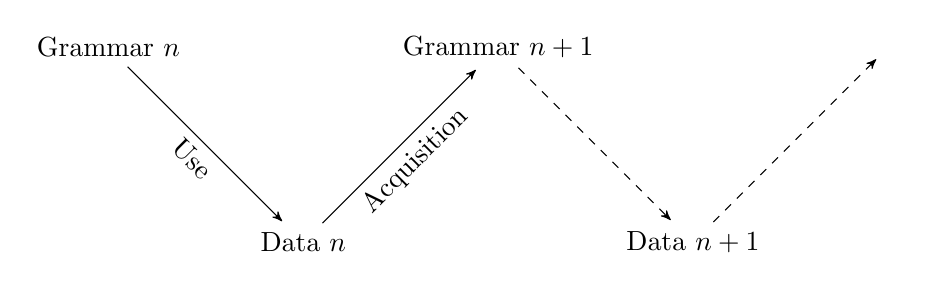
\begin{tikzpicture}[->,>=stealth',shorten >=1pt,auto,node distance=3.5cm]
      \node (A)      {Grammar $n$};
      \node (B) [below right of=A]  {Data $n$};
      \node (C) [above right of=B] {Grammar $n+1$};
      \node (D) [below right of=C] {Data $n+1$};
      \node (E) [above right of=D] {};
      \path[->] (A)  edge node[sloped, anchor=center, below] {Use} (B)
      (B) edge node[sloped, anchor=center, below] {Acquisition} (C)
      (C) edge[dashed] node {} (D)
      (D) edge[dashed] node {} (E);
    \end{tikzpicture}
  \end{center}
\caption{The iterated process of language change through acquisition and use}
\label{change-labeled}
\end{figure}


At the center of this endeavor will be a diachronic process that implicates both use and acquisition, the development in the expression of sentential negation over time known as \emph{Jespersen's cycle} \citeyearpar{jespersen:1917}. The process is often described as the result of two transitions. The first transition occurs when a preverbal form of negation is replaced by an embracing form, which is initially characterized as being more emphatic. The second transition occurs when this embracing form is subsequently replaced by a purely postverbal form. In the history of English, we observe both of these two transition in Middle English from \emph{\textcolor{red}{ne}} to \emph{\color{blue} ne...not} and from \emph{\color{blue} ne...not}  to \emph{\color{green} not}. Our goal will be to determine the role of use and acquisition in each of these transitions.

In Chapter 2 we begin by distinguishing between two phenomena that have often been conflated in investigations of Jespersen's cycle. In particular, we argue that Jespersen's cycle as it is often described consists of both a \emph{formal} and a \emph{functional cycle}. The formal cycle describes the change in the formal complexity of negation over time. It takes place as negation becomes more and then less formally complex, as can be seen in the transitions in the history of English from \emph{\textcolor{red}{ne}} to \emph{\color{blue} ne...not}  to \emph{\color{green} not}. The functional cycle describes the way that different forms of negation are used to signal meaning. It takes place as one form of plain negation  is replaced by another form. This can be seen in the history of English from \emph{\textcolor{red}{ne}} to \emph{\color{blue} ne...not} where the originally empathic \emph{\color{blue} ne...not} displaces \emph{\textcolor{red}{ne}} as it increases in frequency, loses its emphasis, and comes to signal plain negation. We note the logical and empirical relationship between the two cycles: the functional cycle can occur independently of the formal cycle. This result informs the structure of the rest of the dissertation; we start by addressing the functional cycle before turning to the formal cycle.

The first part of this dissertation addresses the functional cycle. In Chapter 3 we introduce the mathematical tools we will use to model the functional cycle. In particular, we show how we can use evolutionary game theory to describe how meaning is signaled in a population over time. Importantly, these tools allow us to model  a qualified kind of Gricean rationality. That is, individuals are \emph{boundedly rational} insofar as they have limited cognitive and informational resources \citep{simon1955,simon1957}. Yet, these tools allow us to show how the actions of individuals can give rise to change at the population level, even when those small decisions are not the product of conscious deliberation \citep{Keller:1994}. This is particularly important when we turn to the functional cycle in Chapter 4, where we show that the first transition from \emph{\textcolor{red}{ne}} to \emph{\color{blue} ne...not} can be explained as the result of speakers' limitations in keeping track of common versus private knowledge.  So, just as Gricean rationality has been used to explain particular patterns of synchronic use, a kind of bounded rationality allows us to explain the functional cycle. So, how we use these two forms explains why they change over time, and the transition from  \emph{\textcolor{red}{ne}} to \emph{\color{blue} ne...not}. 

However, the same model does not apply to the transition from \emph{\color{blue} ne...not}  to \emph{\color{green} not}, so we turn to the formal cycle in the second part of this dissertation. In Chapter 5 we describe a model of syntactic acquisition and determine its predictions for both of the transitions of the formal cycle. In particular, we show that acquisition cannot explain either of the two transitions from  \emph{\textcolor{red}{ne}} to \emph{\color{blue} ne...not} or  from \emph{\color{blue} ne...not}  to \emph{\color{green} not}, other than as the result of a random change in the grammars acquired. In Chapter 6 we test this possibility using statistical methods developed in population genetics to test for random drift versus selection. We find that we can reject random drift in the case of the first transition from \emph{\textcolor{red}{ne}} to \emph{\color{blue} ne...not}, but we cannot reject drift in the case of the second drift from \emph{\color{blue} ne...not}  to \emph{\color{green} not}. This first result suggests that use is the driving force behind the first transition as part of the functional cycle. The second result shows that acquisition does not play a role in any of the observed transitions.  So, insofar as we can offer an explanation of either of the observed changes, we need the notion of pragmatic competence to do so.

%\section{Language Change}
%
%\begin{itemize}
%	\item Language undoubtedly changes
%	\item Weinreich, Labov, Herzog: constraints but not transition or actuation
%	\item What constitutes change? Mental representations
%\end{itemize}
%
%
%A ..theory" of language change in the rigorous sense can be visualized in a relatively strong form and in a weak form. In its strong form, the theory would predict, from a description of a language state at some moment in time, the course of development which that language would undergo within a specified interval. Few practising historians of language would be rash enough to claim that such a theory is possible. In a more modest version, a theory of language change would merely assert that every language constantly undergoes alteration, and it would formulate constraints on the transition from one state of a language to an immediately succeeding state. It might predict further that no language will assume a form in violation of such formal principles as are postulated to be universal in humnan languages. Without predicting positively what will happen (except that the language will somehow change), such a theory would at least assert that some changes will not take place. WLH p.99
%
%The problem of constraints on immediately succeeding language states, to which we alluded above, is in our view subsumed under the broader theoretical question. Of course, we too want to inquire into the set of possible changes and possible conditions for changes which can take place in a structure of a given type. Nor do we want to dismiss the transition problem: it remains entirely relevant to ask about intervening stages which can be observed, or which must be posited, between any two forms of a language defined for a language community at different times. But if the theory is to be illuminating with respect to recorded histories of languages, we must ask two further questons: How are the observed changes embedded in the matrix of linguistic and extralinguistic concomitants of the forms in question? (That is, what other changes are associated with the given changes in
%a manner that cannot be attributed to chance?) And how can the observed changes be evaluated in terms of their effect upon linguistic structure, upon communicative efficiency (as related, e.g., to functional load), and on the wide range of nonrepresentational factors involved in speaking? WLH p.101
%
%\section{Linguistic Explanation}
%
%\begin{itemize}
%	\item Causality : necessary and sufficient conditions
%	\item What counts as an explanation?
%	\item Chomsky: Observational, Descriptive, Explanatory adequacy (Van Frassen: Deductive)
%	\item Description alone is not enough!
%	\item What counts as an explanation in Linguistics?
%\end{itemize}
%
%\section{Causal Forces}
%
%\begin{itemize}
%	\item Need additional evidence that description is grounded in reality somehow.
%	\item We can't rewind and redo language experiments!
%	\item We can note the falsifying cases
%%	\item Stochastic vs deterministic processes
%%	\item Mean dynamics
%\end{itemize}
%
%Languages change. 
%
%Or rather, the mental representations that characterize knowledge change. Somewhere along the iterated chain of language transmission, from one generation to the next, the content of what is learned is substantially different. 
%
%Language change is evidenced by a difference between the linguistic expressions of one generation and the next. Given that the output from one generation serves as the input to the next, both language acquisition and use are crucial to the process of change. While the input to acquisition arises from the interplay of many factors, it is not arbitrary. Rather, it is governed by a \emph{pragmatic competence} that ``underlies the ability to use [\emph{grammatical competence}] along with the conceptual system to achieve certain ends or purposes'' \citep[59]{chomsky1980rules}. In the terms of \cite{chomsky1986knowledge}, the process of language acquisition maps the \emph{E-Language} of one generation to the \emph{I-Language} of the next, whereas pragmatic competence is what governs the mapping from each generation's \emph{I-Language} to its \emph{E-Language}.
%
%In the Gricean tradition \citep{Grice:1975,Levinson:1983, Horn:1984}, this pragmatic competence has been framed in terms of speakers' beliefs, preferences, and intentions. Linguistic expressions are used according to a \emph{Cooperative Principle} whereby interlocutors are taken to make the appropriate contribution to the conversation at the appropriate time towards ``the accepted purpose or direction of the talk exchange'' \citep[26]{Grice:1975}. This framework deftly captures the systematic relationship between what is \emph{said} and what is \emph{meant}, but is clearly an idealization: speakers and hearers might, but need not have the same preferences or goals in a given exchange.   This dissertation aims at understanding the consequences of loosening the assumption of Gricean commonality. It will examine how differences in speakers' and hearers' preferences might impact the use and acquisition of linguistic signals over time. 
%
%At the center of this endeavor will be a diachronic process that implicates both use and acquisition, the development in the expression of negation over time known as \emph{Jespersen's Cycle} \citeyearpar{jespersen:1917}. The main components of this dissertation address the main components of the cycle in turn. First, we consider how the expression of negation transitions from a purely preverbal negator with an optional \emph{emphatic} postverbal element towards a system with obligatory preverbal and postverbal elements. We present a formal model that derives this transition from even a slight preference for exaggeration on the part of speakers. If speakers prefer hearers' response to the emphatic form, then the optional postverbal element will increase in use. On the way up it experiences a kind of \emph{rhetorical devaluation} \citep{dahl:2001}, and is at least partially \emph{bleached} of its emphatic force because, simply put, to ``to emphasize everything is to emphasize nothing'' \citep{kiparsky-condoravdi:2006}. Second, we consider how the expression of negation can shift from the original preverbal negator to the new, increasingly-used, postverbal element. We outline the conditions under which a learner would posit that the postverbal element is a negator in its own right. If the preverbal element appears in contexts where it does not itself express negation, this provides evidence that postverbal element expresses negation and for the eventual loss of the preverbal element entirely. We consider the interaction between these two components of the cycle.
%
%The main contributions of this line of research are the following. First,  it extends recent work in game-theoretic pragmatics that has begun to explore the broader space of possibly divergent preferences \citep{benz-jager-van-rooij:2006, franke:2008, franke-etal:2012, de-jaegher-van-rooij:2013}. This can be taken as a straightforward generalization of the Gricean program to understand the use of linguistic expressions not just as something ``all or most do \emph{in fact} follow but as something that it is \emph{reasonable} for us to follow, that we \emph{should not} abandon'' \citep[29]{Grice:1975}.  Second, it incorporates this perspective into the use of linguistic signals over time. In particular, it suggests how Grice's criterion of reasonability might cut both ways: there are some patterns of use that we \emph{should} and \emph{do} abandon. Differentiating the cases where we expect stability from those where we expect change adds to a broader causal theory of language change \citep{yang2000internal}. 
%
%
%Namely, it offers an additional \emph{internal} force of language change, which derives from a shared pragmatic competence. In the case of Jespersen's Cycle it suggests how morphosyntactic change might arise through a kind of communicative bleaching.   More broadly, it offers insight into the interaction between use and acquisition implicit in the common representation of iterated language change as in Figure \ref{trans}.
%
%\begin{figure}
%\begin{center}
%\begin{tikzpicture}[->,>=stealth',shorten >=1pt,auto,node distance=3cm]
%  \node (A)      {Grammar $n$};
%  \node (B) [below right of=A]  {Data $n$};
%  \node (C) [above right of=B] {Grammar $n+1$};
%  \node (D) [below right of=C] {Data $n+1$};
%  \node (E) [above right of=D] {};
%\path[->] (A)  edge node {} (B)
%  (B) edge node {} (C)
%  (C) edge node {} (D)
%  (D) edge[dashed] node {} (E);
%\end{tikzpicture}
%\end{center}
%\caption{The iterated process of language change through acquisition and use}
%%\label{trans}
%\end{figure}
%
%
%\begin{figure}
%  \begin{center}
%    \begin{tikzpicture}
%      \node (left)      {
\includegraphics[width=.15\textwidth]{left.jpg}};
%      \node (right) [right=4cm  of left] {
\includegraphics[width=.1\textwidth]{right.jpg}};
%      \node (G1) [draw,above=.25cm of left] {Grammar $n$};
%      \path[->] (left)  edge[dashed, out=-35,in=215] node[below]  {Data $n$} (right);
%      \node (G2) [draw,above=.25cm of right] {Grammar $n+1$};
%    \end{tikzpicture}
%  \end{center}
%	\caption{}
%%	\label{acquisition}
%\end{figure}
%
%
%\begin{figure}
%  \begin{center}
%    \begin{tikzpicture}
%      \node (left)      {
\includegraphics[width=.15\textwidth]{left.jpg}};
%      \node (right) [right=4cm  of left] {
\includegraphics[width=.15\textwidth]{right.jpg}};
%      \node (G1) [draw,above=.25cm of left] {Grammar $n$};
%      \node (G2) [draw,above=.25cm of right] {Grammar $n$};
%      \path[->] (left)  edge[dashed, out=-35,in=220] node[below]  {Data $n$} (right);
%      \path[->] (right)  edge[dashed, out=215,in=-40] (left);
%    \end{tikzpicture}
%  \end{center}
%	\caption{}
%	\label{use}
%\end{figure}
%
%
%\begin{figure}
%  \begin{center}
%    \begin{tikzpicture}[->,>=stealth',shorten >=1pt,auto,node distance=3cm]
%      \node (A)      {Grammar $n$};
%      \node (B) [below right of=A]  {Data $n$};
%      \node (C) [above right of=B] {Grammar $n+1$};
%      \node (D) [below right of=C] {Data $n+1$};
%      \node (E) [above right of=D] {};
%      \path[->] (A)  edge node[sloped, anchor=center, below] {Use} (B)
%      (B) edge node[sloped, anchor=center, below] {Acquisition} (C)
%      (C) edge[dashed] node {} (D)
%      (D) edge[dashed] node {} (E);
%    \end{tikzpicture}
%  \end{center}
%\caption{The iterated process of language change through acquisition and use}
%\label{change-labeled}
%\end{figure}
%
%
%
%
%
%The rest of the proposal is structured as follows. Section \ref{Background} offers an overview of Jespersen's Cycle.  We consider the two major approaches to the change, as a \emph{pull-chain} or a \emph{push-chain}. We adopt the latter given that the driving force behind the cycle appears to be pragmatic in nature, stemming from continuous loss and renewal of emphatic negation. We then consider a natural simplification of Eckardt's \citeyear{eckardt2006} analysis of emphatic negation. In Section \ref{Signaling} we develop the mathematical framework that will be used to explicitly connect the analysis of emphatic negation with the cycle. In Section \ref{Cycles} we apply the framework and consider the cycle as a signaling game played in a population where the interests of speakers and hearers slightly diverge. We determine the conditions for the existence of different kinds of equilibria, and the impact of the introduction of new signals under the game dynamics. Finally, in Section \ref{Stability} we 
%determine how the change brought about by use might impact acquisition over time. We suggest different mechanisms that might impact the amount of evidence available to learners at various points in time and how this shapes the trajectory of the change.
%
%\begin{quote}
%	   I am, however, enough of a rationalist to want to find a basis that underlies these facts, undeniable though they may be; I would like to be able to think of the standard type of conversational practice not merely as something that all or most do \textbf{in fact} follow but as something that it is \textbf{reasonable} for us to follow, that \textbf{we should not abandon}. 
% \end{quote}           
%
%\begin{quote}
%As one of my avowed aims is to see talking as a special case or variety of purposive, indeed rational, behaviour, it may be worth noting that the specific expectations or presumptions connected with at least some of the foregoing maxims have their analogues in the sphere of transactions that are not talk exchanges. (Grice 1989, p. 28)
%\end{quote}
%
%\begin{quote}
%[T]o say what a word means in a language is to say what
%it is in general optimal for speakers of that language to
%do with that word, or what use they are to make of it;
%what particular intentions on particular occasions it is
%proper for them to have. Of course, there is no
%suggestion that they always have to have those
%intentions: it would merely be optimal, ceteris paribus,
%for them to have them. (Grice, 1989, p. 299)
%\end{quote}
%
%\begin{quote}
%The maxims do not seem to be coordinate. The maxim
%of Quality [...] does not seem to be just one among a
%number of recipes for producing contributions; it seems
%rather to spell out the difference between something�s
%being, and (strictly speaking) failing to be, any kind of
%contribution at all. False information is not an inferior
%kind of information; it just is not information. (Grice,
%1989, p.371)
%\end{quote}
%
%Conflicts of interest play markedly different roles in Linguistics and Biology. On the one hand, Gricean pragmatics has aimed at understanding the inferences that a listener can draw from a speaker's contribution on the explicit assumption of a shared set of purposes for an exchange. On the other hand, animal signaling has aimed at understanding the existence and persistence of signaling systems in the face of varying degrees of inter- and intra-species conflict.  Both endeavors hinge on the role of conflict, either in its presence or absence. Yet, in the abstract, both deal with the transmission and interpretation of signals. This leads us to consider what happens when we extend our linguistic considerations beyond perfectly aligned interests. 
%
%At first glance, this step outside the idealized realm of common causes yields some forbidding results: conflicts of interest erode communication. The following reasoning, familiar from biological studies of animal signaling, makes clear the root of this unraveling \citep{searcy-nowicki:2005}. Imagine two agents: a sender who sends a signal and a receiver who receives the signal. Suppose that the sender has no incentive to be truthful, in fact, let us suppose that he has every incentive to deceive the receiver. If the sender has an incentive to deceive, then the receiver should not listen. If the receiver does not listen, then the sender has no motive to signal in the first place. Crucially, the actions of the sender depend on those of the receiver and vice versa. Given this interdependence, conflicting interests undermine the information conveyed by signals, rendering them, so to speak, meaningless. 
%
%The same reasoning holds in the case of an entire population of senders and receivers interacting over time. Senders will learn or evolve to dissimulate and receivers will learn or evolve to distrust. This process takes on the familiar form of the \emph{tragedy of the commons} \citep{hardin:1968}. Individuals will always be tempted to exploit the common resource of credulity. Collectively, this incentive to exploit exhausts the resource. Only a fool would tell the truth when there is something to be gained from deception, and only a fool would trust others to be truthful. 
%
%
%\begin{quote}
%	   Make your conversational contribution  such as is required, at the stage at which it occurs, by the accepted purpose or direction of the talk exchange in which you are engaged. One might label this the \textbf{Cooperative Principle}.
%\end{quote}           
%
%
%Silence, or at best meaningless babble, is the equilibrium state in the population: neither senders nor receivers have reason to unilaterally change their behavior. Thomas Schelling's grim pronouncement comes to mind \citep[26]{schelling:1978}:  
%
%\begin{quote}
% The body of a hanged man is in equilibrium when it finally stops swinging, but
%nobody is going to insist that the man is all right.
%\end{quote}
%This sentiment holds doubly. Not only is the inability to convey information problematic, but, we do actually observe informative signaling. The existence of such signaling despite conflicting interests is a genuine puzzle. 
%
%This problem was not lost on Grice, insofar as he recognized the fundamental
%role of his \emph{Maxim of Quality} to the entire enterprise.
%
%\begin{quotation}
%It is obvious that the observance of some of these maxims is a matter of less urgency than is the observance of others; a man who has expressed himself with undue prolixity would, in general, be open to milder comment than would a man who has said something he believes to be false...[O]ther maxims come into operation only on the assumption that this maxim of Quality is satisfied \citep[27]{Grice:1975}
%\end{quotation}
%
%Yet, while we have every incentive to abide by the maxim of Quality when it serves our interests, we have every reason to do otherwise when it does not. So, what keeps human language from the downward spiral to silence? In this regard we can look to animal communication where much work has been devoted to explaining the evolutionary stability of communication. In large part, these solutions take the form of different mechanisms that mitigate conflicts of interest between senders and receivers. 
%
%For example, a sender might guarantee his commitment to the truth by incurring a sufficiently high cost to send a signal. This \emph{handicap principle}  \citep{Zahavi:1975} allows for stable signaling despite conflicting interests.\footnote{See \cite{maynard-smith-harper:2004} and \cite{searcy-nowicki:2005} for thorough discussions of handicaps in animal signaling. Also,\cite{grose:2011} offers a concise but useful discussion of the history and details of the handicap principle. In the economic tradition, \cite{spence:1973} develops a parallel model for educational attainment as a costly signal of job suitability.} To take the usual example, a peacock incurs a cost for his magnificent tail: significant metabolic resources are required to develop the tail, and once developed, his ability to fly is hampered and it makes him more conspicuous to predators. But, successfully bearing the tail serves as a signal of his genetic worth. A weaker peacock would not have been able to support the tail and avoid becoming 
%something else's lunch. Thus, potential mates  can take the tail as a signal of a a truly fit peacock. 
%
%When we turn our attention to language, this sort of mechanism need not be appropriate.  In fact, the notion that truthfulness is enforced by cost is problematic: truth tellers expend as much effort learning and producing their language as liars, and no more. As we say, talk is cheap. There are, of course, various alternatives to handicaps that are appropriate for the case of language \citep{scott-phillips:2008}. A particularly appealing alternative given the social nature of humans, and language, is that of reputation. The minimal requirements for a reputation are the ability of agents to recognize each other individually, keep track of past interactions, and condition future behavior on the outcome of those interactions \citep{Trivers1971}. In the long run, the immediate benefits of deception might not be worth the consequences of a bad reputation.
%
%Abstracting away from the details of the actual mechanisms that mitigate conflict, we can consider three general questions.  First, how effective are these mechanisms in aligning the interests of senders and receivers? Given that language exists, such mechanisms are clearly sufficient to stave off total collapse. However, given that signals are not always used in accordance with the Maxim of Quality, such mechanism are not sufficient to ensure the idealized case of Gricean commonality. Second, if language is indeed subject to a host of competing pressures, what impact will this have on how linguistic signals are used over time?  If not a tragedy of the commons, might we find a lesser \emph{tragedy of the conversation} where particular signals, but not the system as a whole, are destabilized? Third, do we find instantiations of the predicted patterns of language use? In what follows, these second two question will be our chief concern. 
%
%\section{Roadmap}
%
%\begin{enumerate}
%	\item In Chapter \ref{jespersens-cycle} we outline....
%	\item In Chapter \ref{evolutionary-game-theory} we...
%	\item In Chapter \ref{Cycles} we ...
%	\item in Chapter \ref{learning-theory} we...
%	\item in Chapter \ref{Stability}
%	\item in Chapter \ref{conclusion} we summarize our results.
%\end{enumerate}�




%\section{Change}
%
%\begin{itemize}
%	\item Language undoubtedly changes
%	\item What constitutes change? Mental representations
%\end{itemize}
%
%\section{Explanation}
%
%\begin{itemize}
%	\item Causality : necessary and sufficient conditions
%	\item What counts as an explanation?
%	\item Chomsky: Observational, Descriptive, Explanatory adequacy (Van Frassen: Deductive)
%	\item Weinreich, Labov, Herzog: constraints but not transition or actuation
%	\item What counts as an explanation in Linguistics?
%	\item Description alone is not enough!
%\end{itemize}
%
%\section{Causes}
%
%\begin{itemize}
%	\item Need additional evidence that description is grounded in reality somehow.
%	\item We can't rewind and redo language experiments!
%	\item We can note the falsifying cases
%	\item Stochastic vs deterministic processes
%	\item Mean dynamics
%\end{itemize}
%
%Languages change. 
%
%Or rather, the mental representations that characterize knowledge change. Somewhere along the iterated chain of language transmission, from one generation to the next, the content of what is learned is substantially different. 
%
%Language change is evidenced by a difference between the linguistic expressions of one generation and the next. Given that the output from one generation serves as the input to the next, both language acquisition and use are crucial to the process of change. While the input to acquisition arises from the interplay of many factors, it is not arbitrary. Rather, it is governed by a \emph{pragmatic competence} that ``underlies the ability to use [\emph{grammatical competence}] along with the conceptual system to achieve certain ends or purposes'' \citep[59]{chomsky1980rules}. In the terms of \cite{chomsky1986knowledge}, the process of language acquisition maps the \emph{E-Language} of one generation to the \emph{I-Language} of the next, whereas pragmatic competence is what governs the mapping from each generation's \emph{I-Language} to its \emph{E-Language}.
%
%In the Gricean tradition \citep{Grice:1975,Levinson:1983, Horn:1984}, this pragmatic competence has been framed in terms of speakers' beliefs, preferences, and intentions. Linguistic expressions are used according to a \emph{Cooperative Principle} whereby interlocutors are taken to make the appropriate contribution to the conversation at the appropriate time towards ``the accepted purpose or direction of the talk exchange'' \citep[26]{Grice:1975}. This framework deftly captures the systematic relationship between what is \emph{said} and what is \emph{meant}, but is clearly an idealization: speakers and hearers might, but need not have the same preferences or goals in a given exchange.   This dissertation aims at understanding the consequences of loosening the assumption of Gricean commonality. It will examine how differences in speakers' and hearers' preferences might impact the use and acquisition of linguistic signals over time. 
%
%At the center of this endeavor will be a diachronic process that implicates both use and acquisition, the development in the expression of negation over time known as \emph{Jespersen's Cycle} \citeyearpar{jespersen:1917}. The main components of this dissertation address the main components of the cycle in turn. First, we consider how the expression of negation transitions from a purely preverbal negator with an optional \emph{emphatic} postverbal element towards a system with obligatory preverbal and postverbal elements. We present a formal model that derives this transition from even a slight preference for exaggeration on the part of speakers. If speakers prefer hearers' response to the emphatic form, then the optional postverbal element will increase in use. On the way up it experiences a kind of \emph{rhetorical devaluation} \citep{dahl:2001}, and is at least partially \emph{bleached} of its emphatic force because, simply put, to ``to emphasize everything is to emphasize nothing'' \citep{kiparsky-condoravdi:2006}. Second, we consider how the expression of negation can shift from the original preverbal negator to the new, increasingly-used, postverbal element. We outline the conditions under which a learner would posit that the postverbal element is a negator in its own right. If the preverbal element appears in contexts where it does not itself express negation, this provides evidence that postverbal element expresses negation and for the eventual loss of the preverbal element entirely. We consider the interaction between these two components of the cycle.
%
%The main contributions of this line of research are the following. First,  it extends recent work in game-theoretic pragmatics that has begun to explore the broader space of possibly divergent preferences \citep{benz-jager-van-rooij:2006, franke:2008, franke-etal:2012, de-jaegher-van-rooij:2013}. This can be taken as a straightforward generalization of the Gricean program to understand the use of linguistic expressions not just as something ``all or most do \emph{in fact} follow but as something that it is \emph{reasonable} for us to follow, that we \emph{should not} abandon'' \citep[29]{Grice:1975}.  Second, it incorporates this perspective into the use of linguistic signals over time. In particular, it suggests how Grice's criterion of reasonability might cut both ways: there are some patterns of use that we \emph{should} and \emph{do} abandon. Differentiating the cases where we expect stability from those where we expect change adds to a broader causal theory of language change \citep{yang2000internal}. 
%
%
%Namely, it offers an additional \emph{internal} force of language change, which derives from a shared pragmatic competence. In the case of Jespersen's Cycle it suggests how morphosyntactic change might arise through a kind of communicative bleaching.   More broadly, it offers insight into the interaction between use and acquisition implicit in the common representation of iterated language change as in Figure \ref{trans}.
%
%\begin{figure}
%\begin{center}
%\begin{tikzpicture}[->,>=stealth',shorten >=1pt,auto,node distance=3cm]
%  \node (A)      {Grammar $n$};
%  \node (B) [below right of=A]  {Data $n$};
%  \node (C) [above right of=B] {Grammar $n+1$};
%  \node (D) [below right of=C] {Data $n+1$};
%  \node (E) [above right of=D] {};
%\path[->] (A)  edge node {} (B)
%  (B) edge node {} (C)
%  (C) edge node {} (D)
%  (D) edge[dashed] node {} (E);
%\end{tikzpicture}
%\end{center}
%\caption{The iterated process of language change through acquisition and use}
%%\label{trans}
%\end{figure}
%
%
%\begin{figure}
%  \begin{center}
%    \begin{tikzpicture}
%      \node (left)      {
\includegraphics[width=.15\textwidth]{left.jpg}};
%      \node (right) [right=4cm  of left] {
\includegraphics[width=.1\textwidth]{right.jpg}};
%      \node (G1) [draw,above=.25cm of left] {Grammar $n$};
%      \path[->] (left)  edge[dashed, out=-35,in=215] node[below]  {Data $n$} (right);
%      \node (G2) [draw,above=.25cm of right] {Grammar $n+1$};
%    \end{tikzpicture}
%  \end{center}
%	\caption{}
%%	\label{acquisition}
%\end{figure}
%
%
%\begin{figure}
%  \begin{center}
%    \begin{tikzpicture}
%      \node (left)      {
\includegraphics[width=.15\textwidth]{left.jpg}};
%      \node (right) [right=4cm  of left] {
\includegraphics[width=.15\textwidth]{right.jpg}};
%      \node (G1) [draw,above=.25cm of left] {Grammar $n$};
%      \node (G2) [draw,above=.25cm of right] {Grammar $n$};
%      \path[->] (left)  edge[dashed, out=-35,in=220] node[below]  {Data $n$} (right);
%      \path[->] (right)  edge[dashed, out=215,in=-40] (left);
%    \end{tikzpicture}
%  \end{center}
%	\caption{}
%	\label{use}
%\end{figure}
%
%
%\begin{figure}
%  \begin{center}
%    \begin{tikzpicture}[->,>=stealth',shorten >=1pt,auto,node distance=3cm]
%      \node (A)      {Grammar $n$};
%      \node (B) [below right of=A]  {Data $n$};
%      \node (C) [above right of=B] {Grammar $n+1$};
%      \node (D) [below right of=C] {Data $n+1$};
%      \node (E) [above right of=D] {};
%      \path[->] (A)  edge node[sloped, anchor=center, below] {Use} (B)
%      (B) edge node[sloped, anchor=center, below] {Acquisition} (C)
%      (C) edge[dashed] node {} (D)
%      (D) edge[dashed] node {} (E);
%    \end{tikzpicture}
%  \end{center}
%\caption{The iterated process of language change through acquisition and use}
%\label{change-labeled}
%\end{figure}
%
%
%
%
%
%The rest of the proposal is structured as follows. Section \ref{Background} offers an overview of Jespersen's Cycle.  We consider the two major approaches to the change, as a \emph{pull-chain} or a \emph{push-chain}. We adopt the latter given that the driving force behind the cycle appears to be pragmatic in nature, stemming from continuous loss and renewal of emphatic negation. We then consider a natural simplification of Eckardt's \citeyear{eckardt2006} analysis of emphatic negation. In Section \ref{Signaling} we develop the mathematical framework that will be used to explicitly connect the analysis of emphatic negation with the cycle. In Section \ref{Cycles} we apply the framework and consider the cycle as a signaling game played in a population where the interests of speakers and hearers slightly diverge. We determine the conditions for the existence of different kinds of equilibria, and the impact of the introduction of new signals under the game dynamics. Finally, in Section \ref{Stability} we 
%determine how the change brought about by use might impact acquisition over time. We suggest different mechanisms that might impact the amount of evidence available to learners at various points in time and how this shapes the trajectory of the change.
%
%\begin{quote}
%	   I am, however, enough of a rationalist to want to find a basis that underlies these facts, undeniable though they may be; I would like to be able to think of the standard type of conversational practice not merely as something that all or most do \textbf{in fact} follow but as something that it is \textbf{reasonable} for us to follow, that \textbf{we should not abandon}. 
% \end{quote}           
%
%\begin{quote}
%As one of my avowed aims is to see talking as a special case or variety of purposive, indeed rational, behaviour, it may be worth noting that the specific expectations or presumptions connected with at least some of the foregoing maxims have their analogues in the sphere of transactions that are not talk exchanges. (Grice 1989, p. 28)
%\end{quote}
%
%Conflicts of interest play markedly different roles in Linguistics and Biology. On the one hand, Gricean pragmatics has aimed at understanding the inferences that a listener can draw from a speaker's contribution on the explicit assumption of a shared set of purposes for an exchange. On the other hand, animal signaling has aimed at understanding the existence and persistence of signaling systems in the face of varying degrees of inter- and intra-species conflict.  Both endeavors hinge on the role of conflict, either in its presence or absence. Yet, in the abstract, both deal with the transmission and interpretation of signals. This leads us to consider what happens when we extend our linguistic considerations beyond perfectly aligned interests. 
%
%At first glance, this step outside the idealized realm of common causes yields some forbidding results: conflicts of interest erode communication. The following reasoning, familiar from biological studies of animal signaling, makes clear the root of this unraveling \citep{searcy-nowicki:2005}. Imagine two agents: a sender who sends a signal and a receiver who receives the signal. Suppose that the sender has no incentive to be truthful, in fact, let us suppose that he has every incentive to deceive the receiver. If the sender has an incentive to deceive, then the receiver should not listen. If the receiver does not listen, then the sender has no motive to signal in the first place. Crucially, the actions of the sender depend on those of the receiver and vice versa. Given this interdependence, conflicting interests undermine the information conveyed by signals, rendering them, so to speak, meaningless. 
%
%The same reasoning holds in the case of an entire population of senders and receivers interacting over time. Senders will learn or evolve to dissimulate and receivers will learn or evolve to distrust. This process takes on the familiar form of the \emph{tragedy of the commons} \citep{hardin:1968}. Individuals will always be tempted to exploit the common resource of credulity. Collectively, this incentive to exploit exhausts the resource. Only a fool would tell the truth when there is something to be gained from deception, and only a fool would trust others to be truthful. 
%
%
%\begin{quote}
%	   Make your conversational contribution  such as is required, at the stage at which it occurs, by the accepted purpose or direction of the talk exchange in which you are engaged. One might label this the \textbf{Cooperative Principle}.
%\end{quote}           
%
%
%Silence, or at best meaningless babble, is the equilibrium state in the population: neither senders nor receivers have reason to unilaterally change their behavior. Thomas Schelling's grim pronouncement comes to mind \citep[26]{schelling:1978}:  
%
%\begin{quote}
% The body of a hanged man is in equilibrium when it finally stops swinging, but
%nobody is going to insist that the man is all right.
%\end{quote}
%This sentiment holds doubly. Not only is the inability to convey information problematic, but, we do actually observe informative signaling. The existence of such signaling despite conflicting interests is a genuine puzzle. 
%
%This problem was not lost on Grice, insofar as he recognized the fundamental
%role of his \emph{Maxim of Quality} to the entire enterprise.
%
%\begin{quotation}
%It is obvious that the observance of some of these maxims is a matter of less urgency than is the observance of others; a man who has expressed himself with undue prolixity would, in general, be open to milder comment than would a man who has said something he believes to be false...[O]ther maxims come into operation only on the assumption that this maxim of Quality is satisfied \citep[27]{Grice:1975}
%\end{quotation}
%
%Yet, while we have every incentive to abide by the maxim of Quality when it serves our interests, we have every reason to do otherwise when it does not. So, what keeps human language from the downward spiral to silence? In this regard we can look to animal communication where much work has been devoted to explaining the evolutionary stability of communication. In large part, these solutions take the form of different mechanisms that mitigate conflicts of interest between senders and receivers. 
%
%For example, a sender might guarantee his commitment to the truth by incurring a sufficiently high cost to send a signal. This \emph{handicap principle}  \citep{Zahavi:1975} allows for stable signaling despite conflicting interests.\footnote{See \cite{maynard-smith-harper:2004} and \cite{searcy-nowicki:2005} for thorough discussions of handicaps in animal signaling. Also,\cite{grose:2011} offers a concise but useful discussion of the history and details of the handicap principle. In the economic tradition, \cite{spence:1973} develops a parallel model for educational attainment as a costly signal of job suitability.} To take the usual example, a peacock incurs a cost for his magnificent tail: significant metabolic resources are required to develop the tail, and once developed, his ability to fly is hampered and it makes him more conspicuous to predators. But, successfully bearing the tail serves as a signal of his genetic worth. A weaker peacock would not have been able to support the tail and avoid becoming 
%something else's lunch. Thus, potential mates  can take the tail as a signal of a a truly fit peacock. 
%
%When we turn our attention to language, this sort of mechanism need not be appropriate.  In fact, the notion that truthfulness is enforced by cost is problematic: truth tellers expend as much effort learning and producing their language as liars, and no more. As we say, talk is cheap. There are, of course, various alternatives to handicaps that are appropriate for the case of language \citep{scott-phillips:2008}. A particularly appealing alternative given the social nature of humans, and language, is that of reputation. The minimal requirements for a reputation are the ability of agents to recognize each other individually, keep track of past interactions, and condition future behavior on the outcome of those interactions \citep{Trivers1971}. In the long run, the immediate benefits of deception might not be worth the consequences of a bad reputation.
%
%Abstracting away from the details of the actual mechanisms that mitigate conflict, we can consider three general questions.  First, how effective are these mechanisms in aligning the interests of senders and receivers? Given that language exists, such mechanisms are clearly sufficient to stave off total collapse. However, given that signals are not always used in accordance with the Maxim of Quality, such mechanism are not sufficient to ensure the idealized case of Gricean commonality. Second, if language is indeed subject to a host of competing pressures, what impact will this have on how linguistic signals are used over time?  If not a tragedy of the commons, might we find a lesser \emph{tragedy of the conversation} where particular signals, but not the system as a whole, are destabilized? Third, do we find instantiations of the predicted patterns of language use? In what follows, these second two question will be our chief concern. 


% Jespersen's Cycle
\chapter{Jespersen's Cycles}
\label{jespersens-cycles}

\setlength{\epigraphwidth}{.9\textwidth}
\epigraph{The history of negative expressions in various languages makes us witness the following curious fluctuation: the original negative adverb is first weakened, then found insufficient and therefore strengthened, generally through some additional word, and this in its turn may be felt as the negative proper and may then in course of time be subject to the same developments as the original word. \citep[4]{jespersen:1917}}

Originally coined by \cite{dahl:1979}, the term \emph{Jespersen's cycle} is often used in reference to the observation cited above. It is certainly the most quoted aspect of Jespersen's \citeyearpar{jespersen:1917} seminal work, which prefigures many of the current empirical and theoretical issues in the study of negation (cf. \citealt{horn:1989}). Yet, this passage is also interpreted in two very distinct ways. This fundamental ambiguity stems from the fact that Jespersen noted both \emph{formal} and \emph{functional} patterns in the expression of sentential negation over time.\footnote{Sentential negation refers to the semantic property of negating an entire proposition, not just some subpart. It can be distinguished from morphological (e.g. \emph{un-}, \emph{non-}) and constituent negation (e.g. \emph{John might have not understood}) using several diagnostics such as tag questions \citep{klima1964}  and performative paraphrases \citep{payne1985}. Sentential negation is also distinct from but related to the syntactic notion of standard negation \citep{miestamo2005}, which refers to constructions that can reverse the truth value of a proposition.} Both patterns can be conceived of as cycles in their own right. That is, we can find a series of transitions from and back to states that are in some sense formally or functionally equivalent. But, the term Jespersen's cycle is often used in one of these two senses or the other, without clear distinction. 

%There are a range of ways to analyze the syntactic structures underlying the formal cycle. As summarized in part by \cite{vanderAuwera2009}, different analyses have suggested varying levels of detail in the number and realization of stages, ranging from three stages  \citep{burridge1983,bernini-ramat1996,haspelmath1997,frisch1997,zanuttini1997,horn:1989,hoeksma1997,horn2001,roberts-roussou2003,vanderAuwera-neuckermans2004,mazzon2004,willis2005,lucas2007,jager2008,wallage2008}, to four stages \citep{dahl:1979,posner1985,schwegler1988,schwegler1990,ladusaw1993,schwenter2005,schwenter2006}, up to five stages \citep{honda2000,beukema1999,vanderAuwera-neuckermans2004,zeijlstra2004}.  


Perhaps even worse, the canonical presentation of what is referred to as Jespersen's cycle conflates these two uses \citep{posner1985,schwegler1988,schwegler1990,ladusaw1993,schwenter2005,schwenter2006}. Where parentheses at the second stage indicate an optional post-verbal element that is characterized as being emphatic, the following stages are posited.

\begin{center}
\begin{enumerate}
     \item \textsc{\textcolor{red}{neg V}}
    \item  \textsc{\textcolor{red}{neg V} \textcolor{blue}{(neg)}}
    \item \textsc{\color{blue} neg V neg}
    \item \textsc{\color{green} V neg}
\end{enumerate}
\end{center}
This chapter is devoted to defining and distinguishing the two uses of the term intertwined in this representation, which we will call the formal and functional Jespersen cycles. In short, the distinction is between changes in the forms of negation available and changes in how those forms are used to signal meaning, respectively.  Our goal is to clarify the relationship between the two cycles and what would count as an explanation of each.

First, we outline the formal aspects of how negation is expressed at the stages of the formal cycle. We provide a historical description of the structural forms that express negation at different points in the history of English, and compare this trajectory with that of French to emphasize particular aspects of the formal cycle. Second, we outline the function of those forms at different stages of the functional cycle. We provide a historical description of the functions of the different forms at points in the history of both English and French, noting the relationship between optionality and these different functions. We also note the logical relationship between the two cycles: the formal cycle entails the functional cycle, but not vice versa. Third, in light of our definitions and the logical relationship between the two cycles, we discuss two ways of conceptualizing the causes of the cycles and the potential role of syntactic acquisition and pragmatic use in both. 

While the main motivation of this chapter is terminological, distinguishing between the two kinds of cycles has an important consequence. Given the logical relationship between the two cycles, an explanation of the formal cycle requires an explanation of the functional cycle. This informs the structure of the dissertation. Since an explanation of the functional cycle must be our first priority, we begin in Part I by pursuing such an explanation. In Chapter 3 we present a mathematical framework for understanding how different functional meanings are signaled in populations over time. In Chapter 4 we apply this framework to model the functional cycle in the history of English.  With this in place, in Part II we turn to the formal cycle. In Chapter 5 we evaluate a model of syntactic acquisition and the role it might play in an explanation of the formal cycle. In Chapter 6 we consider the possibility that stochastic processes may lead to the transitions in the formal cycle. So, our goal in this chapter is to set the foundation for the rest of the dissertation by clarifying the distinction between the two kinds of cycles.


\section{The formal cycle}

The formal cycle is defined in terms of the forms that are used to express negation over time, and consists of two transitions. At the start of the formal cycle, a single element is used to express negation. The first transition occurs when this single element is supplemented by additional lexical material. The second transition occurs when the original negative element is subsequently lost, leaving the added lexical material as the only expression of negation. In the most general sense, the formal cycle occurs when the form of negation becomes more and then less complex.  It is cyclic in the sense that the forms of negation at the start and end of the cycle are of equal formal complexity. 

This can be shown schematically as in Figure \ref{formal-cycle}, where the vertical axis represents the degree of formal complexity. The first transition takes place from \circled{1} to \circled{2} with the addition of material. The second transition takes place from \circled{2} back to \circled{1} with the loss of material. The addition of material leads to an increase in formal complexity of negation and the loss of material leads to a decrease. The formal cycle is then just a cycle from and back to a less complex form of negation: negation is expressed by some stuff, then more stuff, then less stuff.

%\footnote{We could perhaps be a bit more general by replacing one and two in Figure \ref{formal-cycle} with \circled{$n$} and \circled{$n+1$}, respectively, where $n$ indicates the number of elements used to express negation.} 

\begin{figure}
% Modified from:
% A simple cycle
% Author : Jerome Tremblay
\begin{tikzpicture}
	% Define margin to offset
	\def \margin {8}
	% Draw nodes
	\node[draw,circle] at ({90}:3) {2};
	\node[draw,circle] at ({270}:3) {1};
	% Draw arcs
	\draw[->, >=latex] ({270 - \margin}:3) arc ({270 - \margin}:{90 + \margin}:3);
	\draw[->, >=latex] ({90 - \margin}:3) arc ({90 - \margin}:{-90 + \margin}:3);
	% Draw complexity axis
	\draw[->, >=latex] (-5,-3) -- (-5,3);
	\node[align=center,text width=2cm] at (-6.25, 0) {Formal complexity};
\end{tikzpicture}
\caption{The formal Jespersen cycle}
\label{formal-cycle}
\end{figure}

For example, Jespersen noted that in the history of several European languages, including English and French, a pre-verbal negative element is supplemented by a post-verbal element, and the pre-verbal element is subsequently lost.  This can be shown schematically as in Figure \ref{formal-cycle-spiral} where the different forms of negation are arranged according to formal complexity on the vertical axis and time along the horizontal axis. At both the start and the end of the formal cycle a single element expresses negation. Intuitively, if we abstract away from the structural realization of the forms as pre- or post-verbal, then Figure \ref{formal-cycle-spiral} maps onto Figure \ref{formal-cycle}. The curious fluctuation in form that Jespersen noted simply becomes a closed orbit through the space of formal complexity.

\begin{figure}
\begin{center}
\begin{tikzpicture}[->,>=stealth',shorten >=1pt,auto,node distance=3cm]
  \node (A)      {\textsc{\textcolor{red}{neg V}}};
  \node (B) [above right of=A]  {\textsc{\color{blue} neg V neg}};
  \node (C) [below right of=B] {\textsc{\color{green} V neg}};
  \node (D) [left of=A] {};
  \node (E) [above of=D] {};
\path[->] (A)  edge node {} (B)
  (B) edge node {} (C);
	% Draw axes
    \draw[->] (-1.5,0) -- (-1.5,2);
  \node[align=center, text width=2cm] at (-2.75, 1) {Formal complexity};
    \draw[->] (0,-1) -- (4,-1);
    \node at (2,-1.5) {Time};
\end{tikzpicture}
\end{center}
\caption{The realization of the formal cycle in English and French}
\label{formal-cycle-spiral}
\end{figure}

We see the first stage of the formal cycle in the history of English with the pre-verbal \emph{\textcolor{red}{ne}} in Old English, which expresses sentential negation alone.

\exg. Ic \textcolor{red}{ne} secge\\
      I \textsc{neg} say\\
      (Old English)


This is followed by a stage of embracing or bipartite negation where a post-verbal negative element is added. This is seen in Middle English, where \emph{\textcolor{blue}{ne}} is supplemented by \emph{\textcolor{blue}{not}}.


\exg. I \textcolor{blue}{ne} seye \textcolor{blue}{not}\\
      I \textsc{neg} say \textsc{neg}\\
      (Middle English)

There are several sources that these additional elements are drawn from, most notably from \emph{negative polarity items}, overwhelmingly the set of \emph{minimizers} (e.g. ``not a drop'', ``not a hair'') and \emph{generalizers} (e.g. ``not ever'', ``not at all'', \citealt{horn:1989}). For example, in the case of English, \emph{not} comes from Old English \emph{nawiht} (\emph{literally} ``no thing, creature, being''). Other sources include, indefinite pronouns (e.g. ``no one''), negative adverbs (e.g. ``never'', cf. \citealt{horn:1989,vanGelderen2008negative}), negative verbs (e.g. ``refuse", ``deny", ``reject", ``avoid", ``fail", and ``lack",  \citealt{givon1978}), and the concatenation of negative and existential verbs \citep{croft1991}.


In light of this broad range of sources, it is important to note that the first transition need not consist of the addition of a post-verbal element. For example, in modern African American Vernacular English, negation can be supplemented by a pre-verbal element \emph{eem}, which can express negation in its own right \citep{jones2015}.

\ex. You do\textcolor{blue}{n't eem} know.

\ex. You \textcolor{blue}{eem} know.

As \cite{jones2015} notes, this form comes from but is arguably distinct from \emph{even}.

\ex.  \# \textcolor{blue}{eem} numbers

Importantly, it is the formal status rather than the structural position that is relevant. Given the range of sources for additional negative elements, this is not surprising.  But, it bears emphasis that the transition from pre- to post-verbal negation is not the only path through the formal cycle.  The transition could just as well have been from post- to pre-verbal negation or from and back to pre-verbal negation. It is a contingent historical fact, arising from the syntax of  English and the source of the additional  material, rather than some necessary property of the formal cycle. 

The final stage in the formal cycle is a return to a single negative element. This is seen in Early Modern English, where the preverbal element in \emph{\textcolor{blue}{ne...not}}  is lost, leaving the post-verbal \emph{\textcolor{green}{not}}  as the sole negative element.

\exg. I say \textcolor{green}{not}\\
      I say \textsc{neg}\\
      (Early Modern English)

The emergence of  \emph{do}-support in Early Modern English yields a state parallel to Old English with a sole pre-verbal negator:

\exg. I do \textcolor{red}{not} say\\
      I do \textsc{neg} say\\
      (Present-day English)

The contraction of negation offers an even closer parallel to Old English where \emph{ne} contracted with several verbs (e.g. \emph{ne be} $\rightarrow$ \emph{nis}).

\exg. I do\textcolor{red}{n't} say\\
      I do-\textsc{neg} say\\
      (Present-day English)

But, however suggestive these further developments are, they are not necessary components of the formal cycle.  \citet[10]{jespersen:1917} himself noted the uniqueness of these developments, which he attributed to a tendency to place negation at the beginning of the sentence to avoid confusion. As he put it, the effect of post-verbal negation in German results in a kind of semantic garden path.\footnote{Living is not the highest good (lit. The living is the good highest not)}

\begin{quote}
[T]he hearer or reader is sometimes bewildered at first and thinks that the sentence is to be understood in a positive sense, till suddenly he comes upon the \emph{nicht}, which changes everything; see, for instance ``Das leben ist der g\"{u}ter h\"{o}chstes nicht."
\end{quote}
Yet, despite this purported tendency, the majority of languages that Jespersen noted, including his native Danish, persist in a perplexing state of post-verbal negation. This can only be taken as further evidence that we ought to interpret the implications of Jespersen's observation in formal rather than structural terms. It matters how much stuff is used to express negation, not where that stuff is.

% The transition from purely post-verbal to purely pre-verbal negation is certainly not necessary. For example, German went through a formal cycle in (cf. CHECK \cite{jager2008}), but negation remains purely post-verbal.

% \footnote{The increasing preference of n't over not in colloquial use is illustrated by the use of not contractions of American presidents from Kennedy to Bush. While Kennedy and Nixon still used the uncontracted form not in the majority of cases (during public debates), Bush Sr. and Clinton used this form in only in 14-17\% of all cases (Yaeger-Dror \& Hall-Lew (2002)}

Given the stages of the formal cycle in the history of English, it is useful to give them some historical context. The stages are summarized in Figure \ref{english-timeline}. The horizontal axis represents years in the common era. Immediately above the horizontal axis are commonly-used terms for historical periods: Old English (\emph{ca.} 400-1175 CE), Middle English (\emph{ca.}1175-1450 CE), Early Modern English (\emph{ca.} 1450-1650 CE), and Modern English (\emph{ca.} 1650-Present CE). Above these general time periods are the spans of the different forms of negation.  From Old to Early Modern English we make a full formal cycle from and back to a single negative element. We also see the transition at the end of the formal cycle from post- back to pre-verbal negation in Modern English. 

Below the axis are rough historical anchors that offer a general sense of the historical periods: Beouwulf, the Old English epic poem written some time between 700-1050 CE; Chaucer, the Late Middle English author who is widely-credited as the first to write in the vernacular language of his day, from around 1350-1400 CE; and Shakespeare, the noted dramatist and playwright, from around 1550-1650 CE.


\begin{figure}
\resizebox{\linewidth}{!}{% 
     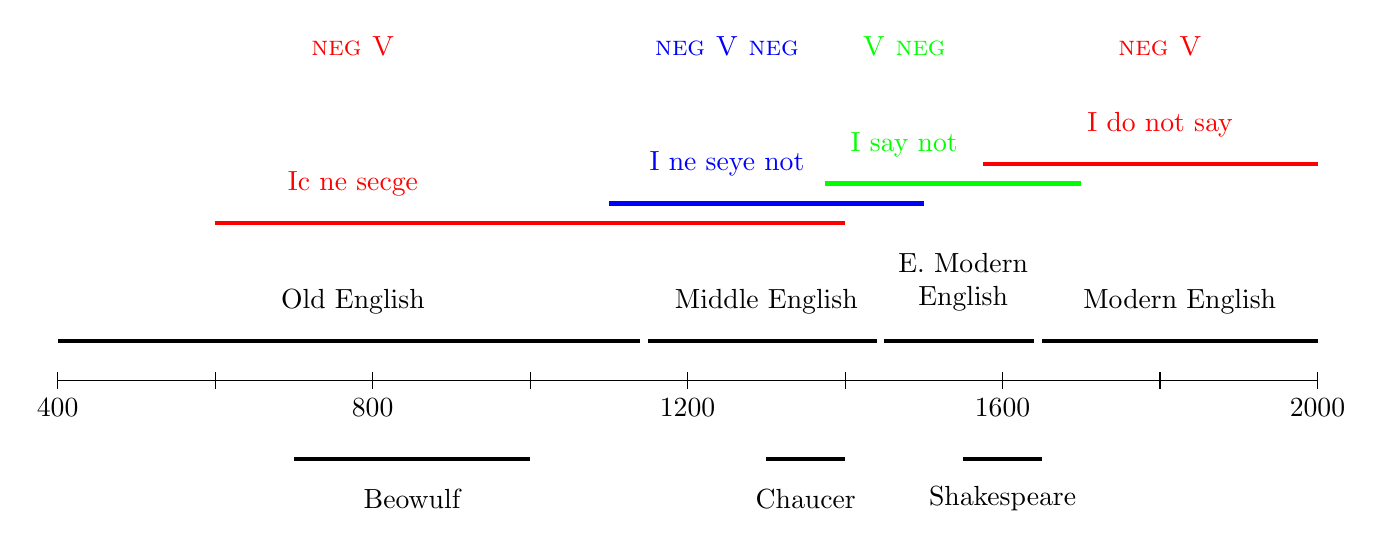
\begin{tikzpicture}
%draw horizontal line
\draw (0,0) -- (16,0);
%draw ticks
\foreach \x in {0, 2, 4, 6, 8, 10, 12, 14, 16}{
   \draw (\x,3pt) -- (\x,-3pt);
}
%draw tick dates
\draw (0,0) node[below=3pt] { 400 } node[above=10pt] { };
\draw (4,0) node[below=3pt] { 800 } node[above=10pt] { };
\draw (8,0) node[below=3pt] { 1200 } node[above=3pt] { };
\draw (12,0) node[below=3pt] { 1600 } node[above=3pt] { };
\draw (16,0) node[below=3pt] { 2000 } node[above=3pt] {  };
% Historical examples
\draw [ultra thick] (3,-1) to (6,-1);
\draw (4.5, -1.5) node {Beowulf};
\draw [ultra thick] (9,-1) to (10,-1);
\draw (9.5, -1.5) node {Chaucer};
\draw [ultra thick] (11.5,-1) to (12.5,-1);
\draw (12, -1.5) node {Shakespeare};
% Add historical languages
% Old English : 400-1175
% Middle English : 1175-1450
% E. Modern English : 1450-1650
% Modern English : 1650-Present
\draw [ultra thick] (0,.5) to (7.4,.5);
\draw (3.75, 1) node {Old English};
\draw [ultra thick] (7.5,.5) to (10.4,.5);
\draw (9, 1) node {Middle English};
\draw [ultra thick] (10.5,.5) to (12.4,.5);
\draw (11.5, 1.25) node[text width=2cm,align=center] {E. Modern English};
\draw [ultra thick] (12.5,.5) to (16,.5);
\draw (14.25, 1) node {Modern English};
% draw ticks for historical examples
% ne 		: 400-1300
% ne..not	: 1100-1400
% not		: 1350-1700
% do not 	: 1500-2000
\draw [ultra thick,red] (2,2) to (10,2);
\draw (3.75, 2.5) node[red] {Ic ne secge};
\draw [ultra thick,blue] (7,2.25) to (11,2.25);
\draw (8.5, 2.75) node[blue] {I ne seye not};
\draw [ultra thick,green] (9.75,2.5) to (13,2.5);
\draw (10.75, 3) node[green] {I say not};
\draw [ultra thick, red] (11.75,2.75) to (16,2.75);
\draw (14, 3.25) node[red] {I do not say};
% draw negative forms
\draw (3.75,4) node [above] {\textsc{\color{red} neg V}};
\draw (8.5,4) node [above] {\textsc{\color{blue} neg V neg}};
\draw (10.75,4) node [above] {\textsc{\color{green} V neg}};
\draw (14,4) node [above] {\textsc{\color{red} neg V}};
\end{tikzpicture}
}
\caption{Timeline of negation in the history of English}
\label{english-timeline}
\end{figure}

The history of negation in French offers a parallel to the formal cycle in English, although the exact details of the timeline are not without dispute (cf. \citealt{martineau-mougeon2003}).  The Old French pre-verbal \emph{\textcolor{red}{ne}} becomes Middle French \emph{\textcolor{blue}{ne...pas}}, and subsequently Modern Colloquial French post-verbal \emph{\textcolor{green}{pas}}.

\exg. Jeo \textcolor{red}{ne} dis\\
      I \textsc{neg} say\\
      (Old French)

\exg. Je \textcolor{blue}{ne} dis \textcolor{blue}{pas}\\
      I \textsc{neg} say \textsc{neg}\\
      (Middle French)

\exg. Je dis \textcolor{green}{pas}\\
      I say \textsc{neg}\\
      (Modern Colloquial French)

Again, it is useful to provide some historical context. The stages of the formal cycle in the history of French are summarized in Figure \ref{french-timeline}. Immediately above the horizontal axis are commonly-used terms for historical periods: Old French (\emph{ca.} 900-1350 CE), Middle French (\emph{ca.}1350-1600 CE), Classical French (\emph{ca.} 1600-1700 CE) , and Modern French (\emph{ca.} 1700-Present CE). Above these general time periods are the spans of the different forms of negation.  From Old to Modern French we make a full formal cycle from and back to a single negative element.

Below the axis are rough historical anchors that offer a general sense of the historical periods: Charlemagne, the first Holy Roman Emperor from 750-800 CE; the Hundred Years' War from roughly 1350-1450 CE; Voltaire, the Enlightenment author and satirist from roughly 1700-1800 CE.


\begin{figure}
\resizebox{\linewidth}{!}{% 
     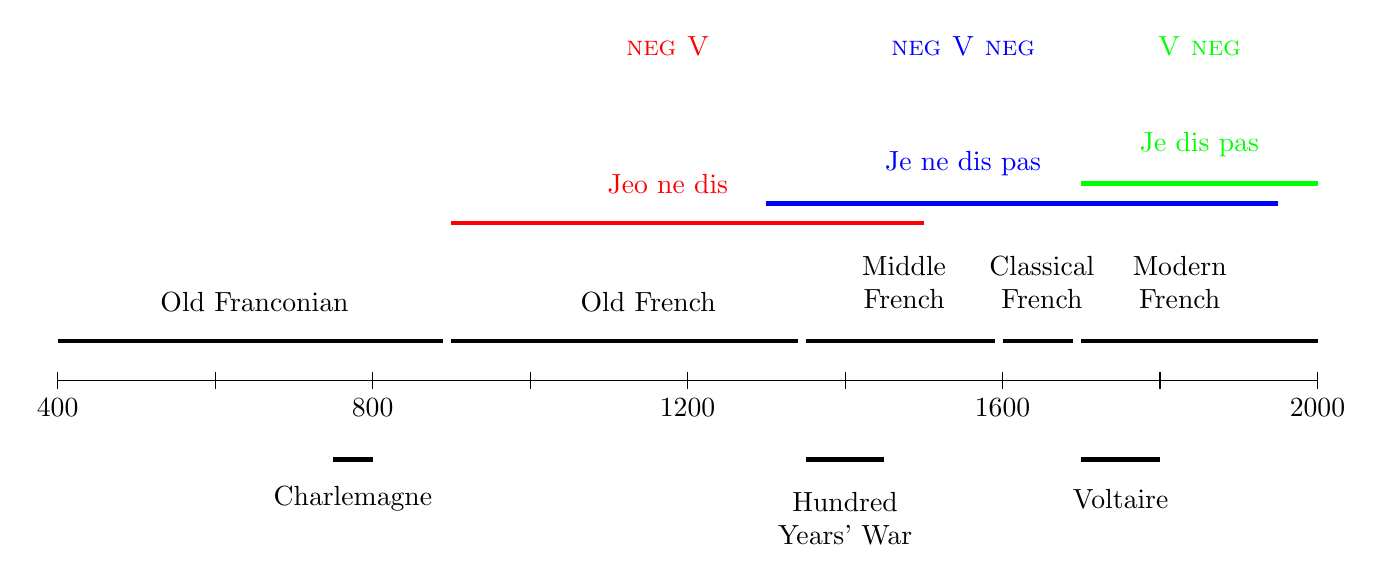
\begin{tikzpicture}
%draw horizontal line
\draw (0,0) -- (16,0);
%draw ticks
\foreach \x in {0, 2, 4, 6, 8, 10, 12, 14, 16}{
   \draw (\x,3pt) -- (\x,-3pt);
}
%draw tick dates
\draw (0,0) node[below=3pt] { 400 } node[above=10pt] { };
\draw (4,0) node[below=3pt] { 800 } node[above=10pt] { };
\draw (8,0) node[below=3pt] { 1200 } node[above=3pt] { };
\draw (12,0) node[below=3pt] { 1600 } node[above=3pt] { };
\draw (16,0) node[below=3pt] { 2000 } node[above=3pt] {  };
% Add historical languages
% Old Franconian : 400-900
% Old French : 900-1350
% Middle French : 1350-1600
% Classical French : 1600-1700
% Modern French : 1700-Present
\draw [ultra thick] (0,.5) to (4.9,.5);
\draw (2.5, 1) node {Old Franconian};
\draw [ultra thick] (5,.5) to (9.4,.5);
\draw (7.5, 1) node {Old French};
\draw [ultra thick] (9.5,.5) to (11.9,.5);
\draw (10.75, 1.25) node[text width=2cm,align=center] {Middle French};
\draw [ultra thick] (12,.5) to (12.9,.5);
\draw (12.5, 1.25) node[text width=2cm,align=center] {Classical French};
\draw [ultra thick] (13,.5) to (16,.5);
\draw (14.25, 1.25) node[text width=2cm,align=center] {Modern French};
% draw ticks for historical examples
% ne 		: 400-1300
% ne..not	: 1100-1400
% not		: 1350-1700
% do not 	: 1500-2000
\draw [ultra thick,red] (5,2) to (11,2);
\draw (7.75, 2.5) node[red] {Jeo ne dis};
\draw (7.75,4) node [above] {\textsc{\color{red} neg V}};
\draw [ultra thick,blue] (9,2.25) to (15.5,2.25);
\draw (11.5, 2.75) node[blue] {Je ne dis pas};
\draw (11.5,4) node [above] {\textsc{\color{blue} neg V neg}};
\draw [ultra thick,green] (13,2.5) to (16,2.5);
\draw (14.5, 3) node[green] {Je dis pas};
\draw (14.5,4) node [above] {\textsc{\color{green} V neg}};
%\draw (14,4) node [above] {\textsc{\color{red} neg V}};
% Historical examples
\draw [ultra thick] (3.5,-1) to (4,-1);
\draw (3.75, -1.5) node {Charlemagne};
\draw [ultra thick] (9.5,-1) to (10.5,-1);
\draw (10, -1.75) node[text width=2.2cm,align=center] {Hundred Years' War};
%\draw [ultra thick] (11,-1) to (12,-1);
%\draw (11.5, -1.5) node {Rabelais};
\draw [ultra thick] (13,-1) to (14,-1);
\draw (13.5, -1.5) node {Voltaire};
\end{tikzpicture}
}
\caption{Timeline of negation in the history of French}
\label{french-timeline}
\end{figure}

\cite{hansen-visconti2009,hansen-visconti2012} note that negation in Louisiana Creole French negation is purely pre-verbal. Of course, this observation comes with the caveat that no conclusions about the future of French can be drawn from this change.

%Although, \cite{hansen-visconti2009,hansen-visconti2012} also note that the post-verbal negator \emph{pas} appears pre-verbally in embedded infinitives \citep{martineau1994}

\exg. Mo \textcolor{red}{pa} di \\
      I \textsc{neg}  say\\
      (Louisiana Creole French)

But again, even if such developments were readily apparent, they would not constitute a necessary component of the formal cycle.
      
Thus, the crucial components of the formal cycle are a transition from one negative element to two, and eventually back to one. For the specific case of English, as well as French, the formal cycle is realized as a transition from pre-verbal to embracing to post-verbal negation. We can represent these transitions schematically as follows.

\begin{center}
\begin{enumerate}
     \item \textsc{\textcolor{red}{neg V}}
    \item \textsc{\color{blue} neg V neg}
    \item \textsc{\color{green} V neg}
\end{enumerate}
\end{center}

Note that these stages are not mutually exclusive. That is, there are transitions between these stages \citep{vanderAuwera2009}.  This captures the theoretical intuition that diachronic change is rarely a dramatic shift. Where parentheses are taken to indicate optionality, the stages can be represented as the following.

\begin{center}
\begin{enumerate}
     \item \textsc{\textcolor{red}{neg V}}
    \item  \textsc{\textcolor{red}{neg V} \textcolor{blue}{(neg)}}
    \item \textsc{\color{blue} neg V neg}
    \item \textsc{\textcolor{blue}{(neg)}  \textcolor{green}{V neg}}    
    \item \textsc{\color{green} V neg}
\end{enumerate}
\end{center}
This more articulated model also comes closer to the diachronic facts. For example, in Late Middle English, all the forms of negation are used contemporaneously: purely pre-verbal, embracing, and post-verbal negation co-occur for a brief period in time. For the moment then, we can take this as the abstract trajectory of the formal cycle over time. 

Importantly, an explanation of the formal cycle in English must consist of two components: it must provide the conditions for the transition from pre-verbal to embracing negation as well as the conditions for the transition from embracing to post-verbal negation. It should be noted that criterion for such explanations can be both qualitative and quantitative. That is, an explanation of the formal cycle can predict both \emph{that} a transition will occur as well as \emph{how} it will occur. In what follows, we will use both kinds of criteria in evaluating models as explanations of change. With this definition of the formal cycle in place, along with what would constitute an explanation for its instantiation in the history of English, we turn to the functional cycle.

%This also occurs synchronically in modern Brazilian Portuguese \citep{schwenter2005, schwenter2006}. 

\section{The functional cycle}

%If the formal cycle is defined by the forms of negation, then the functional cycle is defined by the functions that those forms are put to. It is about how and how many forms are used to mean different things. At the first stage of the cycle one form is generally used to express negation, often characterized as plain negation. Another set of forms is used to express negation in a semantically stronger sense, often characterized as being more emphatic. The first transition in the functional cycle occurs when one of the semantically stronger forms weakens to a strength intermediate between plain and emphatic negation. Thus, at the second stage of the functional cycle the available forms of negation are used to make three functional distinctions. The second transition occurs when the intermediate form weakens even further, coming to have the strength of plain negation, and the original form of plain negation is lost. In the most general sense, the functional cycle occurs when one form of plain negation is replaced by another. It is cyclic in the sense that the number of functionally distinct forms of negation increases then decreases. 

If the formal cycle is defined by the forms of negation, then the functional cycle is defined by the function that those forms are put to. It is about how and how many forms are used to mean different things. At the first stage of the functional cycle a single form is generally used to express negation, often characterized as plain negation. The functional cycle begins with the introduction of another form that is used to express negation in a semantically stronger way, often characterized as being more emphatic. The functional cycle progresses as this new stronger form increases in frequency, weakens, and replaces the original negative form. In the most general sense, the functional cycle occurs when the form of plain negation is replaced by another form. It is cyclic in the sense that the number of functionally distinct forms of negation increases then decreases.

This can be shown schematically as in Figure \ref{functional-cycle} where the vertical axis represents the number of functionally distinct forms of negation. The addition of a new form increases the number of distinctions from \circled{1} to \circled{2}, and the loss of the original form decreases the number of distinctions from \circled{2} back to \circled{1}. However, we should note that Figure \ref{functional-cycle} does not convey all of the necessary information about the functional cycle.

% \footnote{ADD: there aren't JUST two functional distinctions. There are always means of augmenting plain negation to make it emphatic. It might be better to say 2-3-2.}

\begin{figure}
\begin{tikzpicture}
	% Define margin to offset
	\def \margin {8}
	% Draw nodes
	\node[draw,circle] at ({90}:3) {2};
	\node[draw,circle] at ({270}:3) {1};
	% Draw arcs
	\draw[->, >=latex] ({270 - \margin}:3) arc ({270 - \margin}:{90 + \margin}:3);
	\draw[->, >=latex] ({90 - \margin}:3) arc ({90 - \margin}:{-90 + \margin}:3);
	% Draw complexity axis
	\draw[->, >=latex] (-5,-3) -- (-5,3);
	\node[align=center,text width=3cm] at (-6.75, 0) {Functional distinctions};
\end{tikzpicture}
\caption{The functional Jespersen cycle}
\label{functional-cycle}
\end{figure}

Namely, the functional cycle does not hold for just any pair of semantic distinctions. Rather, the incoming form is semantically stronger than the incumbent form. We can more accurately represent the details of the functional cycle as  in Figure \ref{functional-cycle-detail}, where the vertical axis represents semantic strength and the horizontal axis represents time. The original form is supplemented with an additional form that is semantically stronger and this new form weakens over time as it replaces the original from. 

%\footnote{Note that this does not preclude other forms of negation. There are always means for augmenting plain negation to make it emphatic (e.g. `at all', `ever', see \citet[258]{israel2011} and \citet{horn:1989} for incomplete but substantial lists). Crucially the form that is introduced is \emph{more} emphatic than plain negation, but not the only such form.} 

\begin{figure}
\begin{center}
\begin{tikzpicture}[->,>=stealth',shorten >=1pt,auto,node distance=3cm]
  \node[draw,circle] (A)      {1};
  \node[draw,circle] (B) [above right of=A]  {2};
  \node[draw,circle] (C) [below right of=B] {2};
  \node[draw,circle] (D) [below right of=A] {1};
\path[->] (A)  edge node {} (D)
  (B) edge node {} (C);
	% Draw axes
    \draw[->] (-1.5,-2.5) -- (-1.5,2.5);
  \node[align=center, text width=2cm] at (-2.75, 0) {Semantic strength};
    \draw[->] (0,-3) -- (4,-3);
    \node at (2,-3.5) {Time};
%  \node[align=1enter, text width=2cm] at (-2.75, 1) {Formal complexity};
\end{tikzpicture}
\end{center}
\caption{The functional Jespersen cycle in more detail}
\label{functional-cycle-detail}
\end{figure}

The stronger negative form is often a result of elements being added to the original plain form.  For example, in the history of English and French a pre-verbal element is supplemented by a post-verbal element, which strengthens negation. The meaning of the combined pre- and post-verbal elements weakens over time, and the two elements come to have the same force as the original pre-verbal element in isolation. This can be shown schematically as in Figure \ref{functional-cycle-spiral} where the different forms are arranged according to semantic strength along the vertical axis and time along the horizontal axis. If we abstract away from the realization of the particular forms then Figure \ref{functional-cycle-spiral} maps onto Figure \ref{functional-cycle-detail}, which in turn maps onto Figure \ref{functional-cycle}. The curious fluctuation in function that Jespersen noted becomes a particular kind of closed orbit through the space of functional distinctions, which stems from the weakening of negative forms along a semantic dimension.

\begin{figure}
\begin{center}
\begin{tikzpicture}[->,>=stealth',shorten >=1pt,auto,node distance=3cm]
  \node (A)      {\textsc{\textcolor{red}{neg V}}};
  \node (B) [above right of=A]  {\textsc{\color{blue} neg V neg}};
  \node (C) [below right of=B] {\textsc{\color{blue} neg V neg}};
  \node (D) [below right of=A] {\textsc{\textcolor{red}{neg V}}};
\path[->] (A)  edge node {} (D)
  (B) edge node {} (C);
	% Draw axes
    \draw[->] (-1.5,-2.5) -- (-1.5,2.5);
  \node[align=center, text width=2cm] at (-2.75, 0) {Semantic strength};
    \draw[->] (0,-3) -- (4,-3);
    \node at (2,-3.5) {Time};
%  \node[align=1enter, text width=2cm] at (-2.75, 1) {Formal complexity};
\end{tikzpicture}
\end{center}
\caption{The realization of the functional cycle in English and French}
\label{functional-cycle-spiral}
\end{figure}

We see the first stage of the functional cycle in the history of English and French, with pre-verbal \emph{\textcolor{red}{ne}} expressing plain negation.

\exg. Ic \textcolor{red}{ne} secge\\
      I \textsc{neg} say\\
      
\exg. Jeo \textcolor{red}{ne} dis\\
      I \textsc{neg} say\\

The optional addition of a post-verbal element in the embracing forms \emph{\textcolor{blue}{ne...not}} and \emph{\textcolor{blue}{ne...pas}} is used to express a stronger negation.

\exg. I \textcolor{blue}{ne} seye \textcolor{blue}{not}\\
      I \textsc{neg} say \textsc{neg}\\

\exg. Je \textcolor{blue}{ne} dis \textcolor{blue}{pas}\\
      I \textsc{neg} say \textsc{neg}\\

The initial effect of the embracing form, in Jespersen's words \citeyearpar[15]{jespersen:1917}:
%In this case, \emph{not} comes from Old English \emph{nawiht} (\emph{lit.} ``no thing, creature, being''), and indeed has the expected effect. The second stage in the functional cycle in English is evidenced by the use of both \emph{\textcolor{red}{ne}} and \emph{\textcolor{blue}{ne...not}}, where the second has a stronger, emphatic or exaggerative meaning. 

\begin{quotation}
...[I]n most cases the addition serves to make the negative more impressive as being more vivid or picturesque, generally through an exaggeration, as when substantives meaning something very small are used as subjuncts.
\end{quotation}
Despite the evocative phrasing, Jespersen was certainly not the first to notice the trajectory of the functional cycle. It was noted in great detail by both \citet[393]{meillet1912} and \citet[134]{gardiner1904} in French and several other languages.

%o� l�on avait besoin d�insister sur la n�gation [...] on a �t� conduit � renforcer la n�gation ne ... par quelque autre mot. [...] On sait comment pas a perdu, dans les phrases o� il �tait un accessoire de la n�gation, tout sons sens propre�sens conserv� parfaitement dans le mot isol� pas�, comme d�s lors, pas est devenu � lui seul un mot n�gatif, servant � exprimer la n�gation
%\begin{quotation}
%Where we mean to insist upon negation...we are prompted to reinforce the negative \emph{ne}...with some other word....\emph{pas} itself becomes a negative word, used to express negation.
%\end{quotation}

\begin{quotation}
[French \emph{pas} and \emph{point}], from the Latin \emph{passum} and \emph{punctum}, were originally adverbial accusatives placed at the end of negative sentences for the purpose of emphasis; just like the English ``not a jot'', ``not a straw''....\emph{Pas} and \emph{point}, and like them the Demotic B, Coptic AN, next lose their emphasizing force, and become mere adjuncts of the negative words (French \emph{ne}, Coptic 'N). Last of all, they come themselves to be looked upon as negative words.
\end{quotation}
Indeed, \cite{vanderAuwera2009} suggests that \emph{Meillet's spiral} \citeyearpar[394]{meillet1912} may be the more appropriate term for the functional cycle.\footnote{Translation \citet[165]{mcmahon1994}}
%: Les langues suivent ainsi une sorte de d�veloppement en spirale : elles ajoutent des mots accessoires pour obtenir une expression intense : ces mots s�affaiblissent, se d�gradent et tombent au niveau de simples outils grammaticaux ; on ajoute de nouveaux mots ou des mots diff�rents en vue de l�expression ; l�affaiblissement recommence et ainsi sans fin.} 
\begin{quotation}
Thus, languages follow a sort of spiral development: they add extra words to intensify expression; these words fade; decay and fall to the level of simple grammatical tools; one adds new or different words on account of expressiveness; the fading begins again, and so on endlessly.
\end{quotation}

If the functional cycle in English and French begins with the introduction of the optional post-verbal element to create an embracing form that intensifies expression, then it ends when the post-verbal element ceases to be optional. That is, when the post-vebal element becomes obligatory only the embracing form is used, and its intensity fades. This is because the embracing form ceases to be able to signal anything about the distinction between plain and emphatic negation. As \cite{kiparsky-condoravdi:2006} rightly put it, to emphasize everything is to emphasize nothing.  This inverse relation between frequency and informativeness has been argued to underly multiple linguistic phenomena. As forms increase in frequency, they undergo a kind of  \emph{rhetorical devaluation} \citep{dahl:2001}. Simply put, for any form, if it is the only one in use, then it cannot carry any special meaning. There is nothing else to be special in comparison to.

Now that we have defined the formal and functional cycles, there are several important points to be made regarding the relationship between them. First, the effect of one cycle often has implications for the other. For example, the addition of formal material almost always comes with a more restricted and hence stronger meaning.\footnote{The rare exception being truly empty obligatory pleonastic or expletive elements: ``It's raining." Even periphrastic \emph{do}, which is redundant outside of emphatic affirmatives: ``I \textsc{do} want pizza", originally carried some information on its way to becoming obligatory \citep{ecay2015}} This is a natural consequence of how semantic composition proceeds in a generally intersective fashion, to put it set-theoretically. For example, ``a black bear" is certainly more specific, and hence semantically stronger than ``a bear". In the same way, we would expect \emph{\textcolor{blue}{ne...not}} to be more specific in comparison to \emph{\textcolor{red}{ne}}.  This means that the first transition in the formal cycle is virtually guaranteed to coincide with the entirety of a functional cycle, which is indeed what we see in both English and French.

%That is, the functional cycle can occur in the space of a single transition in the formal cycle. This is the case for English and French: the functional cycle ends as the embracing form replaces the pre-verbal element, whereas the formal cycle ends with the subsequent loss of the pre-verbal element.  

Second, the first transition of the formal cycle has a functional cycle tucked inside of it. But, the second transition of the formal cycle does not correspond to another functional cycle. That is, in the case of English and French the transition from embracing to post-verbal negation does not correspond to the same functional trajectory as the preceding transition from pre-verbal to embracing negation. This follows intuitively, again, from the compositional nature of meaning.  The lexical content of the post-verbal form \emph{\textcolor{green}{not}} is a proper subset of the embracing form \emph{\textcolor{blue}{ne...not}}, and thus we would not expect the post-verbal form to have a stronger or more restricted meaning than the embracing form.

%\footnote{The case of modern Brazilian Portuguese offers an interesting potential exception. All three forms, pre-verbal, embracing, and post-verbal are in variation, with the post-verbal meaning having a distinct and more restricted meaning than the other two. We return to this in Chapter 4} 

%We also have historical evidence for the functional difference between the first and second transitions of the formal cycle.
%
%John Palsgrave, an English priest in the court of the infamous serial monogamist Henry VIII, wrote an early grammar of French entitled \emph{L'\'{e}claircissement de la langue francoyse}. The grammar was intended to help his countrymen learn French, and on the subject of negation he wrote the following helpful advice \cite[110]{palsgrave1530}.\footnote{For an electronically-available reprinting published in 1852 see: \url{https://archive.org/details/lclaircissement00wsgoog}}
%
%\begin{quotation}
%For where as they put \emph{ne} before theyr verbes, so often as they expresse negation, like as we use \emph{nat} in our tong after our verbes. They put also after theyr verbes \emph{pas}, \emph{poynt} or \emph{mye}, whiche of theym selfe signifye nothyng, but onely be as signes of negation...there is no verbe that hath \emph{ne} afore him, but he must have either \emph{pas}, \emph{point}, or \emph{mye} after hym...And note that between \emph{pas} and \emph{poynt} there is no maner difference, but it is in the speakers or writtars election whether he wyll use the one or the other. 
%\end{quotation}
%Palsgrave took the embracing form in French to have the same 
%
%Given that Middle English exhibited both embracing and post-verbal negation at the time Palsgrave was born, the lack of distinction between the post-verbal form in English and the embracing form of French is notable. That is, he did not attribute some stronger meaning to the post-verbal form in English in relation to the embracing form. His description also points to the importance of optionality for information. Once the embracing form is obligatory it cannot carry any special meaning above and beyond that of the original pre-verbal form. 



Third, while the functional cycle often takes place within the first transition of the formal cycle, it can occur entirely independently of the formal cycle. For instance, one form can be replaced by another of equal formal complexity.  In Meillet's estimation, the functional cycle is achieved when ``one adds  new \emph{or} different words".  \cite{kiparsky-condoravdi:2006} show that this is exactly what takes place in the history of Greek. Historical forms of negation in Greek are listed in Table \ref{greek-table}, where emphatic negation is taken to be the semantically stronger form in comparison to \emph{plain} negation at any point in time.\footnote{We omit some of the forms for a concise presentation, but see \cite[1]{kiparsky-condoravdi:2006} for a full list. Also, we should note that it is a bit of a misnomer to call any particular form \emph{the} emphatic form. There are always means for augmenting plain negation to make it emphatic (e.g. `at all', `ever', cf. \citet[452]{horn:1989} and \citet[258]{israel2011}). We might think of the forms in Table \ref{greek-table} as \emph{plain} and \emph{frequently-used-but-stronger-than-plain} negation. We return to a particular interpretation of what is meant by \emph{emphasis} in Chapter 4.} The sources of the different forms are ordered chronologically. Importantly, there is a consistent transition of forms between the two functions: the emphatic negation of the last millennium becomes the plain negation of this millennium.

\begin{table}[ht]
    \begin{center}
    \begin{tabular}{@{}ccc@{}}
      \hline
      \textsc{plain} & \textsc{emphatic} & \textsc{source} \\
      \hline
%      ou...ti & ou-de...en & Ancient Greek \\
      \textgreek{ou...ti} & \textgreek{ou-de...en} & Ancient Greek \\
      \textgreek{(ou)den...ti} & \textgreek{den...tipote} & Early Medieval Greek \\
      \textgreek{den...tipote} & \textgreek{den... prama} & Greek Dialects \\
      \textgreek{den...prama} & \textgreek{den...apantoxh} & Modern Cretan \\
      \hline
    \end{tabular}
    \end{center}
    \caption{Historical forms of plain and emphatic negation in Greek}
    \label{greek-table}
\end{table}
Crucially, at least some of these functional cycles occur without any concomitant formal cycle.  For example, if we were to compare the formal complexity of forms after Early Medieval Greek, they would all be equivalent. All of them consist of a shared pre-verbal element \textgreek{den} along with a single post-verbal element. Thus, we see several embracing forms come to express plain negation over time.

Taken together, these points indicate a particular logical relationship between the two cycles. Namely, the formal cycle entails the functional cycle, but not vice versa. This relationship is important because it sets a clear limit on how much an explanation for one kind of cycle can extend to the other. That is, the conditions for the formal cycle can be, at most, sufficient for the functional cycle. In the other direction, the conditions for the functional cycle can be, at most, necessary conditions for the formal cycle. This means that a full understanding of both cycles crucially rests on understanding the functional cycle. 

For now we will largely be concerned with the realization of the functional cycle in English.  The crucial component of the functional cycle is the transition from and back to a single plain form of negation. For the case of English and French, the functional cycle is realized  schematically as the transition from pre-verbal to embracing negation.

%, to two forms that express both plain and a more emphatic negation, back to a single form that expresses the function of plain negation. 
\begin{center}
\begin{enumerate}
     \item \textsc{\textcolor{red}{neg V}}
    \item  \textsc{\textcolor{red}{neg V} \textcolor{blue}{(neg)}}
    \item \textsc{\color{blue} neg V neg}
\end{enumerate}
\end{center}
As we noted above, this leaves out the important detail of semantic strength, but also shows the frequent relation between the functional and formal cycles.  An explanation of the functional cycle in English must consist of one component: it must provide the conditions for the transition from pre-verbal to embracing negation. Note that an explanation of the formal cycle requires an explanation of the functional cycle, but not vice versa. With the definition of both cycles, along with the relationship between them and their explanations, we now turn to two ways of conceptualizing their causes.

% What about an explanation of the first transition of the functional cycle?
% Do we need to explain how the new signal comes to be introduced?

% This relationship between the formal and functional cycles is rather intuitive. Additional lexical material brings additional meaning, but only in one direction. This means that we always find a functional cycle tucked away within each formal cycle. 


\section{Causes of the cycles}

%That is, while some state of affairs may be both necessary and sufficient for the formal cycle, it can only ever be sufficient for the functional cycle. Likewise, while some state of affairs may be both necessary and sufficient for the functional cycle, it need not be necessary or sufficient for the formal cycle.  For our purposes below we will take the functional cycle to coincide with the first transition of the formal cycle. 

We have distinguished between the two kinds of cycles that Jespersen noted. The formal cycle is constituted by a transition from and back to equally complex forms of negation. The functional cycle is constituted by a particular transition from and back to a single form being used to express plain negation. We now consider the two major kinds of scenarios that have been used to conceptualize the causes of the cycles.  Drawing on the terminology of sound change, the two approaches can be though of as \emph{pull-chains} and \emph{push-chains} involving the different forms of negation.

The pull-chain scenario finds its most natural application in the case of the formal cycle, where a new form is \emph{pulled} into expressing negation due to formal weakening. The old form \emph{pulls} in the new form. The push-chain scenario finds its most natural application in the case of the functional cycle, where the old form is pushed out of expressing negation due to functional weakening.  The new form \emph{pushes} out the old form. We assess the plausibility of both scenarios before turning to how different process such as syntactic acquisition and pragmatic use might cause the dynamics of each transition.

%a more general way of formulating the role of different forces in the process of change.

\subsection{A pull-chain scenario}

While Jespersen did not distinguish between the cycles as we have, he did conceive of change as the product of both formal and functional weakening and strengthening.   In particular, he took the role of formal phonetic weakening of the pre-verbal element as a potential cause of change. The clearest interpretation of this cause is in terms of the first transition of the formal cycle. But, it also has potential explanatory power with regards to the second transition.

Regarding the first transition of the formal cycle, Jespersen noted that the pre-verbal elements in English and French were prone to not receiving stress. This creates a problem, insofar as this lack of stress arguably also made negation hard to perceive \cite[5]{jespersen:1917}:

\begin{quotation}
The incongruity between the notional importance and the formal insignificance of the negative (often, perhaps, even the fear of the hearer failing to perceive it) may then cause the speaker to add something to make the sense perfectly clear to the hearer.
\end{quotation}
That is, given the importance of the distinction between affirmation and negation, he reasoned that some additional word is used ``to increase the phonetic bulk'' of the negative signal to bolster its perception \citep[14]{jespersen:1917}. That is, the new embracing form is \emph{pulled} into expressing negation because of the weakness of the purely pre-verbal form.

There are several reasons to be skeptical of this kind of pull-chain scenario. First, phonetic weakening is quite common \citep{bybee2003}. This prevalence suggests that we should be cautious in attributing to it a role in any particular morphosyntactic change. On balance, phonetic weakening is neither necessary nor sufficient for morphosyntactic change.  Second, \citet[547-599]{Labov:1994} offers a thorough critical evaluation of the functional preservation of meaning in the face of sound change. By and large, sound change proceeds in a mechanical fashion without the conscious adjustment to avoid communicative pitfalls. This is true even when such change leads to the loss of the distinction between negation and affirmation. \citet[320]{Labov:2010} notes that in his own native north New Jersey dialect, the pronunciation of the affirmative \emph{can} and the negative \emph{can't} are at times indistinguishable:
\begin{quotation}
	A very common utterance among residents of this Northern New Jersey area was ``Did you say C--A--N or C--A--N--T?,'' since the vowel is tense in both words and the /t/ is often neutralized before a following apical obstruent (as in ``I can't tell you'').
%	 Tense vowels are found in am, an, and as well. I originally cited this as an example of how the advance of sound change can override functional constraints
\end{quotation}
Despite the importance of the functional distinction, no additional material has been added to differentiate the two senses. Third, \cite[177]{posner1985} argues from Italian dialect data that the strength of the pre-verbal form is not correlated with whether the first stage of the formal cycle takes place or not. Taken together, this suggests that a pull-chain scenario is unlikely. Or, at the very least, formal weakening cannot be considered as a necessary or sufficient cause of the first transition of the formal cycle.

Regarding the second transition of the formal cycle, it is useful to note that no such transition takes place in the history of Greek. That is, in Table \ref{greek-table} we see that from Early Medieval Greek onwards there is no formal weakening of either the pre- or post-verbal elements. The crucial difference between the pre-verbal form in those cases and English and French is that the first constitutes a full closed syllable, whereas the second two do not. Thus, while a pull-chain scenario may not offer a causal explanation of the first transition, the role of formal weakness may be important at different stages of the formal cycle. That is, the loss of the pre-verbal element in the transition from the embracing form to the post-verbal form may indeed be related to its formal weight.

%\begin{quote}
%As ne loses its [+NEG] feature, another negative such as not must be present in the clause to contribute the feature [+NEG] at logical form. So, the introduction of not in spec,NegP is not independent in this model. It is a consequence of the loss of [+NEG] on ne.
%
%Weird causality: \citet[649]{wallage2008} "Once ne is no longer associated with the semantic value �negative�, another negative element such as not must be introduced to the clause which has the semantic value �negative�. Hence the ne...not forms we find at stage two of the cycle."
%\end{quote}

\subsection{A push-chain scenario}

%\begin{itemize}
%	\item Push-chain between forms
%	\item Push-chain between elements
%\end{itemize}

Unsurprisingly, Jespersen prefigured the other major conception of the cycle insofar as he took weakening and strengthening to be both formal and functional.   Following Meillet, more recent approaches have focused on the role of functional strengthening and weakening (\citealt{detges-waltereit2002,hopper-traugottt2003,eckardt2006,kiparsky-condoravdi:2006}, \emph{inter alia}). The clearest interpretation of this cause is in terms of the functional cycle as a kind of \emph{push-chain}. 

Crucially, these accounts assume that a stronger form is introduced, increases in frequency due to overuse, and is thus weakened \citep{dahl:2001}. That is, once the new more emphatic form is introduced, its frequency increases due to pragmatic pressures. The subsequent weakening of the new form follows from the information-theoretic properties of signals: to emphasize everything is to emphasize nothing. As the incoming form becomes obligatory, it takes over the expression of plain negation in its own right, \emph{pushing} the original form out.  In the case of English and French, the obligatorification of the post-verbal element pushes the purely pre-verbal form out of the picture.  It should be noted that this push-chain is all that is required to account for the functional cycle. That is, so long as one form of plain negation is replaced by a formerly emphatic form, the functional cycle has occurred. The push-chain ends with the end of the functional cycle. 

This point is important insofar as some analyses have emphasized the completion of the functional cycle as setting the stage for the second transition of the formal cycle. However, these analyses treat the push chain as one between negative elements rather than negative forms. For example, \citet[187]{detges-waltereit2002} argue that the loss of the pre-verbal element follows from a kind of \emph{constructional iconicity} where the simple meaning of plain negation is expressed by a simple form. That is, the sentence just is not big enough for two negative elements. Similarly, \cite{frisch1997} argues that the loss of the pre-verbal element results from the unstable functional doublet created by the use of both \emph{ne} and \emph{not} in \emph{\textcolor{blue}{ne...not}}.  From this viewpoint, \citet[201]{burridge1993} flips the reasoning of the pull-chain, noting that the loss of the pre-verbal element can be seen as the effect, rather than the cause of the addition of the post-verbal element. In a certain sense, this is a kind of functionally-mediated push-chain for the formal cycle. That is, the introduction of the post-verbal element pushes the pre-verbal element out, due to a functional constraint on the number of negative elements in a sentence.

While the notion of simplicity in form to match simplicity in function is a compelling one, it is not a necessary component in understanding the functional cycle as a push-chain. However, this notion may again be helpful in understanding the second transition of the formal cycle. That is, in addition to the formal weight of the pre-verbal element, some preference for a correspondence between form and function may lead to its loss.

\section{Explaining the cycles}

With the mechanics and plausibility of the two kinds of scenarios in mind, it is useful to pause and reconsider what there is to be explained.  Given our focus on the history of negation in English, the empirical facts to explain are the transitions from \emph{\textcolor{red}{ne}} to \emph{\color{blue} ne...not}  and from \emph{\color{blue} ne...not}  to \emph{\color{green} not}. Taken together, these constitute both a functional and formal cycle.  Importantly, we want to understand the role syntactic acquisition and pragmatic use might play in such explanations. 

Before addressing each transition in turn, we note two things. First, both use and acquisition necessarily play a role in any change. This follows from the simple fact that learners have to acquire a language to use it, and other speakers have to use a language for learners to acquire it. So, in a certain trivial sense, both must play some role in language change. In what follows, we will be interested more specifically in the way that use modifies the evidence available to acquisition, and the way that acquisition acts on the evidence from use. Second, our goal is not to explain why forms come about in the first place, but rather how their introduction leads to change. That is, we are not aiming to explain why \emph{\color{blue} ne...not} is introduced into English. We take variation in the forms of negation as a consequence of the broader fact of language variation. 

Regarding the first transition, we noted that we can think of it as a kind of push-chain where the pre-verbal form is being pushed out by the embracing form as it increases in frequency. We are interested in what is causing the increase in the frequency of the embracing form and thus the pushing.  There are at least two possibilities.  First, it could be the case that pragmatic use leads to an increase in the embracing form. This compounds over time to the point where the embracing form is used exclusively. This means that it is the only form present in the linguistic evidence for learners. Thus, learners will only acquire the embracing form. We can represent this schematically as in Figure \ref{first-pragmatic}, where the top row indicates the grammatical knowledge of speakers and the lower row indicates their use of the forms provide by their grammatical knowledge.

\begin{figure}
  \begin{center}
    \begin{tikzpicture}[->,>=stealth',shorten >=1pt,auto,node distance=3.5cm]
      \node (C)  { \emph{\textcolor{red}{ne} \textcolor{blue}{(...not)}} };
      \node (D) [below right of=C] { \emph{\color{blue} ne...not} };
      \node (E) [above right of=D] {\emph{\color{blue} ne...not} };
      \path[->] (C) edge node[sloped, anchor=center, below] {Use} (D)
      (D) edge node[sloped, anchor=center, below] {} (E);
    \end{tikzpicture}
  \end{center}
	\caption{Pragmatic use as the cause of the first transition}
	\label{first-pragmatic}
\end{figure}

So, the upper left \emph{\textcolor{red}{ne} \textcolor{blue}{(...not)}} indicates grammatical knowledge that includes both the pre-verbal and embracing form. We indicate the increase in the embracing form due to use as the downwards arrow in Figure \ref{first-pragmatic}. The result of use is that embracing form is used categorically in the evidence available to subsequent learners. While we only show a single step, this process could just as well be the cumulative effect of use over several iterations. The important things is that use is the force acting to steadily increase the frequency of the embracing form over time, as opposed to acquisition.

While pragmatic pressures are often taken to be the cause of the pushing in the push-chain, there are certainly other options. A second possibility is that syntactic acquisition leads to an increase in the embracing form. This compounds over time to the point where the embracing form is the only one learned. Thus, it is the only one available to speakers to use. We can represent this schematically as in Figure \ref{first-acquisition}, where the top row again indicates grammatical knowledge and the lower indicates the use of forms.

\begin{figure}
  \begin{center}
    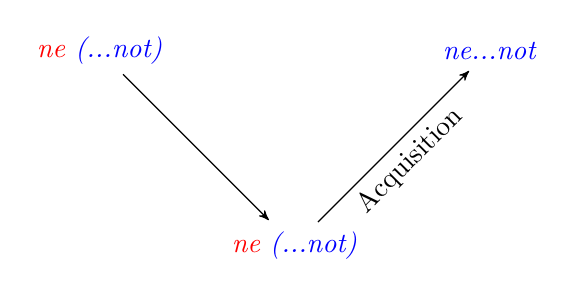
\begin{tikzpicture}[->,>=stealth',shorten >=1pt,auto,node distance=3.5cm]
      \node (C)  { \emph{\textcolor{red}{ne} \textcolor{blue}{(...not)}} };
      \node (D) [below right of=C] { \emph{\textcolor{red}{ne} \textcolor{blue}{(...not)}} };
      \node (E) [above right of=D] {\emph{\color{blue} ne...not} };
      \path[->] (C) edge node[sloped, anchor=center, below] {} (D)
      (D) edge node[sloped, anchor=center, below] {Acquisition} (E);
    \end{tikzpicture}
  \end{center}
	\caption{Syntactic acquisition as the cause of the first transition}
	\label{first-acquisition}
\end{figure}

So, the upper left \emph{\textcolor{red}{ne} \textcolor{blue}{(...not)}} indicates grammatical knowledge that includes both the pre-verbal and embracing form. But, there is no increase in the embracing form due to use. We indicate the increase in the embracing form due to acquisition as the upwards arrow in Figure \ref{first-acquisition}. The result of acquisition is that only the embracing form is acquired.  Again, while we only show a single step, this could just as well be the result of several iterations. Crucially, it is acquisition rather than use that is driving the increase in the embracing form. 

While we can present these two causes in isolation, another possibility is that both use and acquisition interact over time, giving rise to the embracing form. However, the important thing in any case is the form that an explanation must take. That is, for pragmatic use or syntactic acquisition to serve as explanations of the first transition we must demonstrate how they cause the increase in the frequency of the embracing form. We need a model of use or acquisition that makes both qualitative and quantitative predictions. That is, we need a model that predicts \emph{that} the first transition will happen, as well as \emph{how} it will happen.

The same requirements holds for the second transition.  We can represent what a pragmatic or syntactic explanation would like in Figures \ref{second-pragmatic} and \ref{second-acquisition}. For either to serve as an explanation, we would have to demonstrate how they cause the increase in \emph{\color{green} not} over time. Note that these requirements are independent of whether it makes sense to conceive of the second transition as a push-chain or whether we think that use or acquisition play any role whatsoever. In fact, it serves as an important check on any models we posit for the first transition. For example, if we have no reason to think that pragmatic use is what drives the second transition, then a model of the first transition based on use should not predict the second transition. 

\begin{figure}
  \begin{center}
    \begin{tikzpicture}[->,>=stealth',shorten >=1pt,auto,node distance=3.5cm]
      \node (C)  { \emph{\textcolor{blue}{(ne...)} \textcolor{green}{not}} };
      \node (D) [below right of=C] { \emph{\color{green} not} };
      \node (E) [above right of=D] {\emph{\color{green} not} };
      \path[->] (C) edge node[sloped, anchor=center, below] {Use} (D)
      (D) edge node[sloped, anchor=center, below] {} (E);
    \end{tikzpicture}
  \end{center}
	\caption{Pragmatic use as the cause of the second transition}
	\label{second-pragmatic}
\end{figure}


\begin{figure}
  \begin{center}
    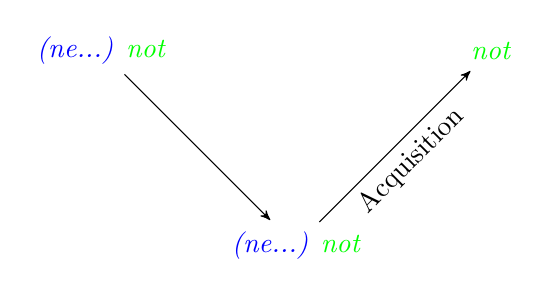
\begin{tikzpicture}[->,>=stealth',shorten >=1pt,auto,node distance=3.5cm]
      \node (C)  { \emph{\textcolor{blue}{(ne...)} \textcolor{green}{not}} };
      \node (D) [below right of=C] { \emph{\textcolor{blue}{(ne...)} \textcolor{green}{not}} };
      \node (E) [above right of=D] {\emph{\color{green} not} };
      \path[->] (C) edge node[sloped, anchor=center, below] {} (D)
      (D) edge node[sloped, anchor=center, below] {Acquisition} (E);
    \end{tikzpicture}
  \end{center}
	\caption{Syntactic acquisition as the cause of the second transition}
	\label{second-acquisition}
\end{figure}


\section*{Summary}

In this chapter we made the important terminological distinction between the formal and functional Jespersen cycles and noted the logical relationship between the two phenomena. An explanation of the formal cycle requires an explanation of the functional cycle, but not vice versa. importantly, given that the functional cycle can occur independently of the formal cycle, an explanation of the first may be fundamentally different from an explanation of the second. This guides our approach to explaining the two processes in the history of English, observed as the transitions from \emph{\textcolor{red}{ne}} to \emph{\color{blue} ne...not}  to \emph{\color{green} not}. 

In Part I we pursue an explanation of the functional cycle based on pragmatics. We present a mathematical framework for modeling how meaning is signaled in a population over time and apply it to modeling how pragmatic use leads to the transition from \emph{\textcolor{red}{ne}} to \emph{\color{blue} ne...not}, but not the transition from  \emph{\color{blue} ne...not}  to \emph{\color{green} not}. In Part II we turn to the formal cycle as a whole and evaluate whether a model of syntactic acquisition can explain either of the transitions, from \emph{\textcolor{red}{ne}} to \emph{\color{blue} ne...not} and from \emph{\color{blue} ne...not}  to \emph{\color{green} not}.



%\chapter{Jespersen's Cycle (20 pages)}
%
%\setlength{\epigraphwidth}{.9\textwidth}
%\epigraph{The history of negative expressions in various languages makes us witness the following curious fluctuation: the original negative adverb is first weakened, then found insufficient and therefore strengthened, generally through some additional word, and this in its turn may be felt as the negative proper and may then in course of time be subject to the same developments as the original word. \citep[4]{jespersen:1917}}
%
%Originally coined by \cite{dahl:1979}, the term \emph{Jespersen's Cycle} refers to the observation cited above regarding the expression of negation over time for several European languages. In particular, Jespersen noted a particular pattern in the history of negation in Danish, English, and French. In what follows we will focus on the history of negation in English. The reasons for focusing on English are threefold. First, we have historical records of sufficient time depth, from Old English (The York-Toronto-Helsinki Parsed Corpus of Old English Prose (YCOE), \cite{ycoe}) through Middle English (The Penn-Helsinki Parsed Corpus of Middle English (PPCME2), \cite{ppcme2})  and beyond (The Penn-Helsinki Parsed Corpus of Early Modern English, (PPCEME) \cite{ppceme}, The Penn-York Computer-annotated Corpus of a Large amount of English based on the TCP (PYCCLE), \cite{pyccle}).  Second, these corpora provide sufficient data to investigate both qualitative and quantitative aspects of change. Third, and closely related to the second motivation, negation is sufficiently frequent to be amenable to both qualitative and quantitative analysis.
%
%In the rest of this chapter we present two interpretations of Jespersen's observation. It bears noting that Jespersen took the change in negation he observed to be a matter of both \emph{formal} and \emph{functional} weakening and strengthening, although subsequent work has often emphasized only or the other dimension. Here we address both aspects of the change. First, we outline the \emph{formal} aspects of how negation is expressed. Namely, we provide a description of the structural forms that express negation at different points in time. Second, we outline the \emph{function} of those forms at. That is, we describe the meaning of the different forms of negation at different points in time. Finally, we discuss how these two aspects of the cycle relate to change over time. 
%
%Before doing so, we should note that more recent work has established the cross-linguistic prevalence of similar patterns of change in various language families beyond Indo-European, including Uralic, Na-Dene, and Afro-Asiatic languages \textit{inter alia} (cf. \citet{vanGelderen2008negative}). The variety of patterns has led some to suggest the broader and more pluralistic term \emph{Negative Cycles} \cite{vanGelderen2008negative}.  In what follows we will focus on the history of negation in English, and use the more restricted term \emph{Jespersen's Cycle}. While the analyses presented here may hold more generally for diachronic patterns of negation, the underlying phenomena may be substantially different, requiring 
%different approaches. The resources available for English make it the ideal test case for studying Jespersen's Cycle. While the analyses presented in subsequent chapters can and must eventually be extended to other languages to gain empirical footing, English will serve as a starting point.
%
%\section{Form}
%
%
%The first stage is that of purely preverbal negation. This is seen in Old English and Old French, where \emph{\textcolor{red}{ne}} expresses negation alone.
%
%\exg. Ic \textcolor{red}{ne} secge\\
%      I \textsc{neg} say\\
%      (Old English)
%
%
%This is followed by a stage of embracing or bipartite negation where a postverbal negative reinforcer is added. This is seen in Middle English, where \emph{\textcolor{blue}{ne}} is reinforced by \emph{\textcolor{blue}{not}}.
%
%
%\exg. I \textcolor{blue}{ne} seye \textcolor{blue}{not}\\
%      I \textsc{neg} say \textsc{neg}\\
%      (Middle English)
%
%Elements recruited to induce emphasis are by and large \emph{negative polarity items}, overwhelmingly drawn from the set of \emph{minimizers} (e.g. ``not a drop'', ``not a hair'') and \emph{generalizers} (e.g. ``not ever'', ``not at all'', \citealt{horn:1989}). These can be seen in the examples of the cycle in English and French above. In the case of English, ``not'' comes from Old English ``nawiht'' (\emph{literally} ``no'' + ``thing, creature, being''). In the case of French, ``pas'' comes from ``step'', and in fact still has this separate meaning in non-negative contexts. Other sources include, but are not limited to indefinite pronouns (e.g. ``no one'') and negative adverbs (e.g. ``never'') (cf. \citealt{horn:1989,vanGelderen2008negative}).
%
%\cite{givon1978} adds a second source: �negative mark- ers [...] most often arise, diachronically, from erstwhile negative main verbs, commonly �refuse�, �deny�, �reject�, �avoid�, �fail�, or �lack� �.
%
%\cite{croft1991}  discusses a related cyclical development, namely how the negative and existential verb are merged together and used as a negative.
%
%Finally, there is the stage of purely postverbal negation. This is seen in Early Modern English, where the preverbal negator in \emph{\textcolor{blue}{ne...not}}  is lost, leaving \emph{\textcolor{green}{not}}  as the sole negator.
%
%\exg. I say \textcolor{green}{not}\\
%      I say \textsc{neg}\\
%      (Early Modern English)
%
%In Present-day English there seems to have been a partial re-establishment of the initial state due to the loss of V-to-T raising, the emergence of \emph{do}-support, and the contraction of negation.
%
%\exg. I do \textcolor{red}{not} say\\
%      I do \textsc{neg} say\\
%      (Present-day English)
%
%\exg. I do\textcolor{red}{n't} say\\
%      I do-\textsc{neg} say\\
%      (Present-day English)
%
%
%\begin{figure}
%\resizebox{\linewidth}{!}{% 
%     \begin{tikzpicture}
%%draw horizontal line
%\draw (0,0) -- (16,0);
%%draw ticks
%\foreach \x in {0, 2, 4, 6, 8, 10, 12, 14, 16}{
%   \draw (\x,3pt) -- (\x,-3pt);
%}
%%draw tick dates
%\draw (0,0) node[below=3pt] { 400 } node[above=10pt] { };
%\draw (4,0) node[below=3pt] { 800 } node[above=10pt] { };
%\draw (8,0) node[below=3pt] { 1200 } node[above=3pt] { };
%\draw (12,0) node[below=3pt] { 1600 } node[above=3pt] { };
%\draw (16,0) node[below=3pt] { 2000 } node[above=3pt] {  };
%% Historical examples
%\draw [ultra thick] (3,-1) to (6,-1);
%\draw (4.5, -1.5) node {Beowulf};
%\draw [ultra thick] (9,-1) to (10,-1);
%\draw (9.5, -1.5) node {Chaucer};
%\draw [ultra thick] (11.5,-1) to (12.5,-1);
%\draw (12, -1.5) node {Shakespeare};
%% Add historical languages
%% Old English : 400-1175
%% Middle English : 1175-1450
%% E. Modern English : 1450-1650
%% Modern English : 1650-Present
%\draw [ultra thick] (0,.5) to (7.4,.5);
%\draw (3.75, 1) node {Old English};
%\draw [ultra thick] (7.5,.5) to (10.4,.5);
%\draw (9, 1) node {Middle English};
%\draw [ultra thick] (10.5,.5) to (12.4,.5);
%\draw (11.5, 1.25) node[text width=2cm,align=center] {E. Modern English};
%\draw [ultra thick] (12.5,.5) to (16,.5);
%\draw (14.25, 1) node {Modern English};
%% draw ticks for historical examples
%% ne 		: 400-1300
%% ne..not	: 1100-1400
%% not		: 1350-1700
%% do not 	: 1500-2000
%\draw [ultra thick,red] (2,2) to (10,2);
%\draw (3.75, 2.5) node[red] {Ic ne secge};
%\draw [ultra thick,blue] (7,2.25) to (11,2.25);
%\draw (8.5, 2.75) node[blue] {I ne seye not};
%\draw [ultra thick,green] (9.75,2.5) to (13,2.5);
%\draw (10.75, 3) node[green] {I say not};
%\draw [ultra thick, red] (11.75,2.75) to (16,2.75);
%\draw (14, 3.25) node[red] {I do not say};
%% draw negative forms
%\draw (3.75,4) node [above] {\textsc{\color{red} neg V}};
%\draw (8.5,4) node [above] {\textsc{\color{blue} neg V neg}};
%\draw (10.75,4) node [above] {\textsc{\color{green} V neg}};
%\draw (14,4) node [above] {\textsc{\color{red} neg V}};
%\end{tikzpicture}
%}
%
%\caption{Timeline of negation in the history of English}
%\label{timeline}
%\end{figure}
%
%
%A more articulated model captures the intuition that there are transitions between these stages \citep{vanderAuwera2009}. That is, between the purely preverbal and embracing negation there is a period of optional embracing negation; between the obligatory embracing negation and purely post-verbal negation there is a period of optional embracing negation. Where parentheses are taken to indicate optionality, the stages can be represented schematically as the following.
%
%\begin{center}
%\begin{enumerate}
%     \item \textsc{\color{red} neg V}
%%    \item \textsc{n V (n)}
%    \item \textsc{\color{blue} neg V neg}
%%    \item \textsc{(n) V n}
%    \item \textsc{\color{green} V neg}
%\end{enumerate}
%\end{center}
%Note that this does not preclude the coexistence of all three forms synchronically. For example, we do indeed find instances of all three forms in variation: \textsc{n V} $\sim$ \textsc{n V n} $\sim$ \textsc{V n} \citep{schwenter2005, schwenter2006}. We might then, at least for the moment, consider this a general trajectory over time.
%
%\begin{itemize}
%	\item Three stages : \citep{burridge1983,bernini-ramat1996,haspelmath1997,zanuttini1997,horn:1989,hoeksma1997,horn2001,roberts-roussou2003,vanderAuwera-neuckermans2004,mazzon2004,willis2005,lucas2007,jager2008} 
%	\item Four stages : \citep{dahl:1979,schwegler1988,schwegler1990,schwenter2005,schwenter2006}
%	\item Five stages : \citep{honda2000,beukema1999,vanderAuwera-neuckermans2004,zeijlstra2004}
%\end{itemize}
%%Five stages
%% Zeijlstra (2004), Willis (2005)
%
%
%\exg. Jeo \textcolor{red}{ne} dis\\
%      I \textsc{neg} say\\
%      (Old French)
%
%\exg. Je \textcolor{blue}{ne} dis \textcolor{blue}{pas}\\
%      I \textsc{neg} say \textsc{neg}\\
%      (Middle French)
%
%\exg. Je dis \textcolor{green}{pas}\\
%      I say \textsc{neg}\\
%      (Present-day Colloquial French)
%
%
%
%\begin{figure}
%\resizebox{\linewidth}{!}{% 
%     \begin{tikzpicture}
%%draw horizontal line
%\draw (0,0) -- (16,0);
%%draw ticks
%\foreach \x in {0, 2, 4, 6, 8, 10, 12, 14, 16}{
%   \draw (\x,3pt) -- (\x,-3pt);
%}
%%draw tick dates
%\draw (0,0) node[below=3pt] { 400 } node[above=10pt] { };
%\draw (4,0) node[below=3pt] { 800 } node[above=10pt] { };
%\draw (8,0) node[below=3pt] { 1200 } node[above=3pt] { };
%\draw (12,0) node[below=3pt] { 1600 } node[above=3pt] { };
%\draw (16,0) node[below=3pt] { 2000 } node[above=3pt] {  };
%% Add historical languages
%% Old Franconian : 400-900
%% Old French : 900-1350
%% Middle French : 1350-1600
%% Classical French : 1600-1700
%% Modern French : 1700-Present
%\draw [ultra thick] (0,.5) to (4.9,.5);
%\draw (2.5, 1) node {Old Franconian};
%\draw [ultra thick] (5,.5) to (9.4,.5);
%\draw (7.5, 1) node {Old French};
%\draw [ultra thick] (9.5,.5) to (11.9,.5);
%\draw (10.75, 1.25) node[text width=2cm,align=center] {Middle French};
%\draw [ultra thick] (12,.5) to (12.9,.5);
%\draw (12.5, 1.25) node[text width=2cm,align=center] {Classical French};
%\draw [ultra thick] (13,.5) to (16,.5);
%\draw (14.25, 1.25) node[text width=2cm,align=center] {Modern French};
%% draw ticks for historical examples
%% ne 		: 400-1300
%% ne..not	: 1100-1400
%% not		: 1350-1700
%% do not 	: 1500-2000
%\draw [ultra thick,red] (5,2) to (11,2);
%\draw (7.75, 2.5) node[red] {Jeo ne dis};
%\draw (7.75,4) node [above] {\textsc{\color{red} neg V}};
%\draw [ultra thick,blue] (9,2.25) to (15.5,2.25);
%\draw (11.5, 2.75) node[blue] {I ne seye not};
%\draw (11.5,4) node [above] {\textsc{\color{blue} neg V neg}};
%\draw [ultra thick,green] (13,2.5) to (16,2.5);
%\draw (14.5, 3) node[green] {I say not};
%\draw (14.5,4) node [above] {\textsc{\color{green} V neg}};
%%\draw (14,4) node [above] {\textsc{\color{red} neg V}};
%% Historical examples
%\draw [ultra thick] (3,-1) to (4,-1);
%\draw (3.5, -1.5) node {Charlemagne};
%\draw [ultra thick] (6,-1) to (7,-1);
%\draw (6.5, -1.75) node[text width=2.2cm,align=center] {\emph{La Chanson de Roland}};
%\draw [ultra thick] (11,-1) to (12,-1);
%\draw (11.5, -1.5) node {Rabelais};
%\draw [ultra thick] (13,-1) to (14,-1);
%\draw (13.5, -1.5) node {Voltaire};
%\end{tikzpicture}
%}
%\caption{Timeline of negation in the history of French}
%\label{french-timeline}
%\end{figure}
%
%\section{Function}
%
%\begin{itemize}
%	\item Jespersen basically provided a shotgun explanation
%	\item Gardiner and Meilet predate him wrt the functional explanation
%	\item How are we to interpret the causation of the cycle
%\end{itemize}
%
%
%
%\begin{quotation}
%L� o� l�on avait besoin d�insister sur la n�gation [...] on a �t� conduit � renforcer la n�gation ne ... par quelque autre mot. [...] On sait comment pas a perdu, dans les phrases o� il �tait un accessoire de la n�gation, tout sons sens propre�sens conserv� parfaitement dans le mot isol� pas�, comme d�s lors, pas est devenu � lui seul un mot n�gatif, servant � exprimer la n�gation 
%Where we needed to insist on negation [...] it was taken to strengthen the negation ... by any other word. [...] We know how not lost, in sentences where he was an accessory to the denial, all clean-sense meaning sounds perfectly preserved in the isolated word pas- as not therefore became in itself a negative word used to express negation
%(Meilet 1913: p.393)
%\end{quotation}
%
%\begin{quotation}
%Les langues suivent ainsi une sorte de d�veloppement en spirale : elles ajoutent des mots accessoires pour obtenir une expression intense : ces mots s�affaiblissent, se d�gradent et tombent au niveau de simples outils grammaticaux ; on ajoute de nouveaux mots ou des mots diff�rents en vue de l�expression ; l�affaiblissement recommence et ainsi sans fin.
%Thus, languages follow a sort of spiral development: they add extra words to intensify expression; these words fade; decay and fall to the level of simple grammatical tools; one adds new or different words on account of expressiveness; the fading begins again, and so on endlessly.
%(Meilet 1912: p394, translation McMahon 1994: p.165)
%
%\end{quotation}
%
%\begin{quotation}
%These words, from the Latin passum and punctum, were originally adverbial
%accusatives placed at the end of negative sentences for the purpose of emphasis; just
%like the English �not a jot�, �not a straw�. [...] Pas and point, and like them the
%Demotic B , Coptic AN, next lose their emphasizing force, and become mere adjuncts of F
%the negative words (French ne, Coptic 'N). Last of all, they come themselves to be looked upon as negative words. (Gardiner 1904: 134)
%\end{quotation}
%
%\section{Causes}
%
%
%Thus, the cyclic nature of the cycle can be attributed to an eventual return to original syntactic state. However, in Present-day Colloquial French there has yet to be such a change towards the original syntactic state of purely preverbal negation. Nor is any such return guaranteed to occur. It seems strange to call something a cycle if it never returns to the point of origin. A resolution to this conceptual problem lies in considering the potential causes of the cycle. The two approaches in the literature regarding the cause of the change can be summarized as \emph{push-chains} and \emph{pull-chains}.
%
%\section{Pull-Chain}
%In Jespersen's own words, the transition between the stages is a matter of \emph{weakening} and \emph{strengthening}.
%
%\begin{quotation}
%The history of negative expressions in various languages makes us witness the following curious fluctuation: the original negative adverb is first weakened, then found insufficient and therefore strengthened, generally through some additional word, and this in its turn may be felt as the negative proper and may then in course of time be subject to the same developments as the original word. \citep[4]{jespersen:1917} 
%\end{quotation}
%In the case of a pull-chain analysis, the preverbal negation has a tendency to not receive main stress and thus becomes a clitic. Given the importance of the distinction between affirmation and negation, some additional word is used ``to increase the phonetic bulk'' of the negative signal to bolster its perception \citep[14]{jespersen:1917}. That is, some new marker is \emph{pulled} into expressing negation because of the weakening of the original preverbal negator.
%
%The prevalence of phonetic weakening suggests we should be skeptical of its role in any particular morphosyntactic change. There is ample evidence of phonetic weakening not leading to morphosyntactic change, and morphosyntactic change in the absence of any precursory phonetic weakening. More pertinent to the case at hand, \cite{posner1985} argues from Italian dialect data that apparently weak preverbal negators are not necessarily supplemented by some additional element. If phonetic weakening is not sufficient for the cycle, then this suggest that a pull-chain scenario is unlikely.
%
%\section{Push-Chain}
%
%Perhaps unsurprisingly, Jespersen prefigured the other major conception of the cycle insofar as he took weakening and strengthening to be both phonetic and semantic in nature.  In the latter case, which Jespersen thought to be the more frequent, some additional word is used ``to make the negative more impressive as being more vivid or picturesque'' \citep[15]{jespersen:1917}. This intuition is exactly what more recent theories have referred to as emphasis (\citealt{detges-waltereit2002, hopper-traugottt2003, eckardt2006, kiparsky-condoravdi:2006}, \emph{inter alia}).  More precisely, the incoming form of embracing negation is emphatic in comparison to the original form of preverbal negation. 
%
%On this second account, the increasing use of the postverbal emphatic element eventually leads to its loss of emphatic force. As \cite{kiparsky-condoravdi:2006} so eloquently note, ``to emphasize everything is to emphasize nothing.'' The directionality of the change then proceeds from the introduction of the post verbal element and its transition towards being obligatory. The new element potentially takes over the expression of negation in its own right, \emph{pushing} the original negator out. While this approach to the cycle often takes the loss of the preverbal negator as a given, it should be noted that this is most definitely not guaranteed. That is, while the postverbal element may increase in frequency and lose its emphasis, it need not necessarily come to be the sole expression of negation and push the preverbal element out. As a case in point, \cite{kiparsky-condoravdi:2006} present evidence from the history of Greek for the stability of a single preverbal negator over multiple centuries alongside 
%several postverbal elements that first convey emphatic and then plain negation. This provides further evidence that a pull-chain scenario is untenable given that phonetic weakening is neither necessary nor sufficient for the cycle.
%
%The push-chain scenario, however, offers a new perspective on the pull-chain mechanism. That is, it suggests the phonetic reduction of the preverbal element not as the cause of the change, but rather as an effect of it. The phonetic bulk of the preverbal negator may be crucial in determining if and when the expression of negation is identified elsewhere. For example, a less substantial element might not be perceived, yielding evidence that it does not express negation, whereas a more substantial element might provide  sufficient evidence for its status as the expression of negation. It is unsurprising that the relevant preverbal negator in Greek constitutes a heavy syllable, which would arguably have enough phonetic heft to be identified.
%
%Additionally, the push-chain suggests a particular interpretation of what is being pushed. That is, the form of plain negation is being pushed out by the form of emphatic negation. The cycle can be thought of as  essentially semantico-pragmatic in nature. It stems from the loss and renewal of emphatic negation due to pragmatic pressures.  This is obviously not to say that the relevant morphosyntactic repercussions are unexpected; the surprising cross-linguistic regularity of occurrence is what prompted Jespersen's original observation. Rather, it suggests that the use of negation under pragmatic pressures can, and often does have morphosyntactic consequences. In what follows we will consider the implications of this characterization of the cycle. We start with a characterization of emphatic negation.
%
%
%%\section{Emphatic Negation}
%
%Elements recruited to induce emphasis are by and large \emph{negative polarity items}, overwhelmingly drawn from the set of \emph{minimizers} (e.g. ``not a drop'', ``not a hair'') and \emph{generalizers} (e.g. ``not ever'', ``not at all'') \citep{horn:1989}. These can be seen in the examples of the cycle in English and French above. In the case of English, ``not'' comes from Old English ``nawiht'' (\emph{literally} ``no'' + ``thing, creature, being''). In the case of French, ``pas'' comes from ``step'', and in fact still has this separate meaning in non-negative contexts. Other sources include, but are not limited to indefinite pronouns (e.g. ``no one'') and negative adverbs (e.g. ``never'') (cf. \citealt{horn:1989,vanGelderen2008negative}).
%
%\cite{eckardt2006} draws on a variant of the analysis presented in \cite{krifka1995polarity} to give a particularly appealing account of how these NPIs are used to express emphatic negation. The basic intuition is that emphatic negation arises through the occurrence of NPIs under emphatic focus.  Theories of \emph{focus} draw on the notion of alternatives, incorporating what could have been said into the computation of focus sensitive construction \citep{rooth1992}. NPIs pick out extremal elements of the relevant set of alternatives, and emphasis indicates that this choice is in some sense surprising. This account recommends itself not only because it integrates the relevant material into the compositional machinery of the semantics, but it does so through independently motivated mechanisms. We present the two components of this account in turn, following Eckardt's exposition unless otherwise noted. We then offer a slightly simpler means of deriving the impact of emphatic negation.
%
%The first component of Eckardt's account draws on the notion of alternatives induced by focus. In addition to the ordinary semantic interpretation, an expression $E$ also has a focus driven semantic interpretation. We can represent the first by \inter{E}$^o$ and the second by \inter{E}$^f$. The ordinary interpretation of an expression is as would be expected given the usual semantic machinery. In contrast, the focus  driven interpretation is sensitive to the presence of an abstract focus feature $f$. The focus driven interpretation of the abstract focus feature yields a set consisting of the ordinary semantic value of the expression and the set of salient alternatives in the context: $\{F_1, F_2, F_3...\}$.  Thus, the presence or absence of a focus feature gives rise to the following possibilities.
%
%\ex. \inter{E}$^f$ $= \{\inter{E}^o\} $
%
%\ex. \inter{E_f}$^f$ $= \{\inter{E}^o, F_1, F_2, F_3...\} $
%
%The set of alternatives is restricted to be of the same logical type as the expression. So, for example, nouns evoke alternative entities, transitive verbs evoke binary relations between entities, and so forth. In essence, this simply captures the intuition that the realization of focus generates a set of alternatives when it occurs, but has no effect when it does not. Similarly, the abstract focus feature is, so to speak, invisible to the ordinary semantic interpretation.
%
%Computing the meaning of a complex expression $AB$, which contains a focus marked element, is accomplished by the following  rule of evaluation, where $\infty$ indicates a suitable method of semantic composition, 
%
%\ex. \inter{AB}$^f = \{ A_i \infty B_j | A_i \in \inter{A}^f, B_j \in \inter{B}^f \} $
%
%When no subexpression is focus marked, this simply results in ordinary semantic composition. That is, the focus driven interpretation simply yields the normal functional application, or predicate modification, of the two subexpressions. When a subexpression is focus marked this generates a set of alternatives, which then all undergo the appropriate semantic composition.
%
%As a simple example, consider the following sentence where $f$ indicates the abstract focus feature, which is reflected in English prosody via prominent stress.
%
%\ex. John$_f$ knows the number.
%
%The components of the sentence are then the following, supposing that the individuals in the context are John, Joe, and Jim.
%
%\ex. \inter{John_f}$^f = \{ \inter{John}^o, Joe, Jim \} = \{ John, Joe, Jim \}$
%
%\ex. \inter{\text{knows the number}}$^f = \{ \inter{\la x . know(x, \text{the number})}^o \} = \{ \la x . know(x, \text{the number}) \}$
%
%The composition that results yields the set of alternatives of all individuals that could know the number.
%
%\ex. \inter{\text{knows the number}}$^f$(\inter{John_f}$^f) = \{$ John knows the number, Joe knows the number, Jim knows the number $\}$
%
%
%The second component of Eckardt's account is the notion of emphatic assertion. In this case, the resulting effect of emphatic assertion is taken to be akin to a tacit ``even''.  For example, consider the following sentence.
%
%\ex. Even John$_f$ knows the number.
%
%In addition to the assertion that John indeed knows the number, it implicates that all of the alternatives are also true, and, most importantly, that the asserted proposition is the most surprising or striking of all the alternatives.
%
%It is this last aspect which is taken to be crucial in emphatic assertions. The effect of emphasis can be encoded as an operator, the application of which yields both the asserted content, the ordinary semantic interpretation of the sentence, along with an implicature regarding the relation between the asserted content and all its alternatives. Where $P$ is taken as some measure of expectation in a given context, the effect can be represented as the following.\footnote{This is a trivial reformulation of \cite{eckardt2006}, which is a slight departure from that of \cite{krifka1995polarity}. The latter requires that the asserted statement be more surprising than the conjunction of all other alternatives. Nothing hinges on this difference, but here we adopt the less stringent criterion.}
%
%\ex. \textbf{emph}(S) \\ asserts: \inter{S}$^o$ \\ implicates: $\forall S' \in \inter{S}^f . P(\inter{S}^o) \leq P(\inter{S'}^o)$
%
%That is, an emphatically asserted utterance carries with it the implicature that it is somehow surprising or unexpected in comparison to its alternatives.
%
%With both components, we can evaluate a sentence with an NPI.
%
%\ex. Anna did not drink [a single drop]$_f$
%
%This sentences gives rise to the set of alternative propositions.
%
%\ex. \inter{S}$^f$ = $\{$ `Anna did not drink a single drop', `Anna did not drink a glassful', `Anna did not drink a barrelful', `Anna did not drink a swimming pool-ful'...$\}$
%
%Emphatically asserting this sentence leads to the implication that, of these alternatives, the proposition that is actually asserted is the most striking or unexpected.
%
%\ex. \textbf{emph}(Anna did not drink [a single drop]$_f$) \\ asserts: Anna did not drink a single drop. \\ implicates: This is surprising or unexpected relative to what she could have drunk.
%
%NPIs generate alternatives through focus, and emphatic focus leads to the implication that the asserted proposition is surprising or unexpected in comparison to its alternatives. Taken together, these components allow for the effects of emphatic negation to be derived pragmatically.
%
%While these components together yield the desired effect of emphatic negation, a perhaps more parsimonious account lies in the nature of the alternatives generated by NPIs. That is, unlike the alternatives induced by focus marking of an individual, NPIs introduce alternatives that are ordered along a scale according to semantic entailment.
%
%Scales underpin our reasoning about the relationship between ordered sets of propositions. For example, imagine a set of puzzles ordered by degree of increasing difficulty: $y_1 < y_2 < ... < y_n$. Positive and negative claims regarding an individual's ability to solve a particular puzzle allow for inferences regarding that same individual's ability to solve other puzzles. For example, consider the following.
%
%\ex. John can solve puzzle $y_i$.
%
%\ex. John can't solve puzzle $y_i$.
%
%From the first, we can infer that John can solve all easier puzzles; he can solve $y_j$ for all $j \leq i$. From the second, we can infer that John cannot solve any harder puzzles; he cannot solve $y_j$ for any $j \geq i$. The latter contexts are \emph{scale-reversing} allowing inferences from low values on the scale to high values, whereas the former are \emph{scale-preserving} allowing inferences from high values on the scale to low values \citep{fauconnier1975}.
%
%NPIs pick out the low end of a particular scale and allow us to reason about propositions higher in the scale. In contrast with ordinary negation, emphatic negation signals two things \citep{kadmon-landman1993any}. First, there is a reduced tolerance to exceptions. For example, in the case of a cook making dinner for a large group of people, the amount of potatoes that would be relevant is quite large. We can imagine the following exchange.
%
%  \ex. \a. Will there be French fries tonight?
%       \b. No, I don't have potatoes.
%       \b. Maybe you have just a couple of potatoes that I could fry in my room.
%       \b. Sorry, I don't have \textsc{any} potatoes.
%
%Emphasis \emph{widens} the interpretation of potatoes from quantities relevant to a large group to quantities relevant to even a single person.
% 
%Second, emphasis yields a stronger statement. For example, in the case of the following threats, the latter is clearly the stronger prohibition.
%
%  \ex. \a. If you move, I'll shoot.
%       \b. If you budge an inch, I'll shoot.
%
%It is clear that either form of the threat allows for a certain amount of pragmatic slack in interpretation: being shot for blinking would seem rather ungenerous. However, there is still a clear relationship between the two. While scratching an itch might not be advisable in either situation, it as at least less inadvisable under the former than the latter. In all those situations where the first threat would be carried out we would expect the second to be as well, but not vice versa. In this sense, emphasis \emph{strengthens} the interpretation of a given statement.
%
%The basic intuition that connects the two effects of NPIs is that they signal something about how strictly the meaning is to be interpreted (cf. \citealt{lewis1970,landman1991}). In the examples above, this determines what it means to have potatoes or what counts as moving. We will refer to this contextually determined value as the \emph{standard of precision}. Such standards of precision stand in a particular relation to each other \citep{krifka1995polarity}. Namely, for two standards of precision, $t_i$ and $t_j$, we might say that one is stricter than the other, $t_i \prec t_j$ just in case the extensions of a given property, $\alpha$, is preserved under a loosening of the standard. 
%
%\ex. $t_i \prec t_j$ if and only if $\alpha_j \subset \alpha_i$
%
%This simply means that anything that holds at a stricter standard holds at a looser standard, but not necessarily vice versa. So, not having potatoes for a single person means that you still do not have enough potatoes for fifty people. But, not having potatoes for fifty people does not mean that you do not have enough for just one person. Likewise, scratching an itch might not get you shot at the looser standard, but it certainly could at the stricter one.
%
%Intuitively, an NPI makes negation emphatic because it signals a stricter standard than might be normally expected. It suggests that the speaker has evidence for making the assertion even under some stricter standard of interpretation. While plain negation might be compatible with a wide range of standards, emphatic negation picks out a much narrower range standards. Namely, it picks out an extremely high standard, if not the highest. In this sense, emphatic negation is surprising because it is particularly informative relative to plain negation \citep{israel1998,israel2001}. This is, of course, not an immutable fact about emphatic negation. It is exactly the loss of informativity that is at the center of Jespersen's Cycle. The question is then why emphatic negation, and the information it conveys, are subject to this continual erosion. In the next section we will lay out a formal framework for exploring this question.

\part{Cycles}

% Evolutionary Game Theory
\chapter{Evolutionary Game Theory}
\label{evolutionary-game-theory}

\setlength{\epigraphwidth}{.9\textwidth}
\epigraph{We repeat most emphatically that our theory is thoroughly static. A dynamic theory would unquestionably be more complete and preferable.\\ --\citet[44-45]{von-neumann-morgenstern1944}\\ \hspace{12pt}

We shall now take up the ``mass-action'' interpretation of equilibrium points...It is unnecessary to assume that the participants have full knowledge of the total structure of the game, or the ability and inclination to go through any complex reasoning process.\\
--\citet[21]{nash1950}
%There are many situations, however, in which an individual is, in effect, competing not against an individual opponent but against the population as a whole.\\ --\citet[23]{maynard-smith1982}
}

Game theory is a branch of applied mathematics originally developed by \cite{von-neumann-morgenstern1944} that models human decision-making when the actions, outcomes, and preferences of multiple agents are intertwined. This differs from decision theory, where a single agent is faced with a choice to bring about his or her most preferred outcome. Rather, a game arises when the choices made by each player crucially depend on those made by others. It is this interdependence that distinguishes game theory and makes it such a useful tool in understanding social interactions, from the routes we choose to drive to work to the way we use words to mean things.

The rest of this chapter provides an outline of the crucial concepts for our application of evolutionary game theory to language change. First, we offer a general overview of the dimensions along which games vary. We focus on two simple games, and develop intuitions about expected behavior. Second, we define a set of solution concepts that can be applied to predict behavior in the two simple games. We discuss the limitations of solutions concepts for predicting behavior. Third, we supply game dynamics and examine the trajectory of the population under those game dynamics for the two simple games. We then we define signaling games as a natural model of communication and present the simplest case. Finally, we present a generalized means of describing the dynamics of arbitrarily complex signaling games.

\section{The role of rationality}

Taking up one aspect of this first example, we will assume that the vast majority of people would prefer to avoid car accidents. When driving a car, this is straightforwardly achievable by always being on the opposite side of the road of the next oncoming vehicle. We can think about this from the perspective of two drivers approaching each other. Each driver has the choice of driving on the left or the right. Both parties would prefer to coordinate on driving on whichever side. The side of the road that best achieves the outcome of not crashing is irrelevant, but it depends on how both parties drive. If both parties choose to drive on the right, from their own perspective, then they will avoid each other. Likewise if they choose to drive on the left.

The solutions to this interaction are readily apparent, everyone should choose one side of the road or the other. Provided that both drivers choose the same side, then neither has an incentive to switch. This fundamental insight into behavior in games is what defines a \emph{Nash equilibrium}: the action of all agents is optimal given the choices of all other agents. Yet, grounding this solution in rationalistic terms requires a little more effort. First, it requires that all agents are \emph{rational}, acting to maximize their own benefit. This is implicit in our example above, most humans prefer to avoid being injured. Second, it requires that players have \emph{common knowledge} of the game structure, including the actions available to all players, the outcomes of different combinations, and know that they all know these things, and so forth. At least for this game it follows naturally from the number of sides of the road there are, and the ability to reason about collisions, but it is not always so straightforward. Finally, it requires that agents have \emph{equilibrium knowledge}, that they are able to accurately anticipate the actions of other players.  This last requirement may seem readily apparent, at least for the example of driving, but it deserves further comment. 

Depending on the country, we know that everyone will drive on one side of the road. In fact, there are laws and legal repercussion for not doing so. Yet, if we abstract away from our everyday experience in this particular case, the problem becomes clearer. For example, imagine that you are asked to choose between two options, that another person has been asked to choose between the same two options, that both of you have received the same instructions, and that you will both succeed if you choose the same option. These starker terms may seem to border on the absurd, but they bring the problem into relief. Their absurdity lies in the fact that it does not do to reason about \emph{this} option or \emph{that} option, because there is nothing to distinguish the two. There is no \emph{thisness} or \emph{thatness} to motivate one choice or the other. That is, there is no rule of the road that simply states "Drive on the right". Instead, we are faced with the problem of deciding the undecidable, as Aristotle, a bit sarcastically put it in his \emph{On the Heavens}:
%Buridanian 

\begin{quotation}
%men who, though exceedingly hungry and thirsty, and both equally, yet being equidistant from food and drink, is therefore bound to stay where he is-even so
[A] man, being just as hungry as thirsty, and placed in between food and drink, must necessarily remain where he is and starve to death.
\end{quotation}

We are particularly good at looking for reasons why one option is preferable, or more likely to be chosen than another. For example, if we were to enrich our description above to a choice between an option \emph{A} or an option \emph{B}, an intuitive rationale would be to choose \emph{A}. The reason for doing so being that \emph{A} comes first in the alphabet, and that both people might expect each other to know this. There is some intuitive \emph{thisness} about option \emph{A} that we can leverage on the assumption that it will be readily apparent to others as well.  \citet[57]{schelling:1960} called these partial escapes from the dilemma of equilibrium knowledge \emph{focal points} ``for each person's expectation of what the other expects him to expect to be expected to do." In the pre-cellular age, Schelling posed the following scenario: ``Tomorrow you have to meet a stranger in NYC. Where and when do you meet them?" The intuitive meeting place of Schelling's day was Grand Central station at noon. The rationale for both choices is that they are prominent in their respective geographical and temporal landscapes. Experimental results demonstrate that people are generally quite  good at grounding their coordination via reasoning about these kinds of focal points \citep{mehta-etal1994,mehta-etal1994b,bardsley-etal2010}. 


But, even with our ability to reason about what we might expect others to expect us to expect them to expect us to do, we still cannot perfectly anticipate what others will do. That is, focal points are useful heuristics, but they are never foolproof: not everyone would choose option \emph{A} or grand central station at noon. In fact, it would not be foolish for example to suggest meeting at Times Square at noon. The problem of justifying equilibrium in general still remains. Nash himself was well aware of this problem, which was in part what prompted his consideration of a ``mass-action'' interpretation of equilibria.\footnote{The main motivation was understanding \emph{mixed Nash equilibria}, which involve some probability distribution over actions. \cite{nash1950,nash:1950,nash:1951} proved that such an equilibrium is guaranteed to exist. What it means for an individual to adopt the corresponding \emph{mixed strategy} is not unproblematic. For a discussion of these problems see \cite{aumann1985}, and for the population approach see \cite{rosenthal1979}.} In short, this change in perspective moves from focusing on a single agent to a population of agents that need not have either common knowledge or equilibrium knowledge.  This perspective was naturally taken up in applications of game theory to biology, where loosening some of the equilibrium requirements was both reasonable and necessary \citep{maynard-smith1982}. This move also came with the reinterpretation of the game-theoretic machinery: actions were not choices to be made by the individual, but genetically pre-determined responses; the utility derived from a particular outcome was not a numerical representation of preferences, but a measure of Darwinian \emph{reproductive fitness}. 

This turn towards the biological allowed for further developments towards the explicitly dynamic theories that \cite{von-neumann-morgenstern1944} envisioned.  Drawing on the mechanics of population genetics, \cite{taylor-jonker:1978} offered the first \emph{evolutionary game dynamics}, christened the \emph{replicator dynamics} by  \cite{eigen-schuster1979}, which explicitly defined how a population changes over time due to biological reproduction.  This new approach allowed for insights into not just whether a population would remain at some equilibrium state if it started there, but also if the population would reach that equilibrium state in the first place. While successively detailed refinements of Nash equilibria were proposed with more and more unrealistic assumptions, evolutionary game theory offered a means of understanding equilibrium behavior under much simpler assumptions. 

Despite its biological roots, however, work in evolutionary game theory has discovered profound connections with the rationalistic approach to equilibrium behavior. That is, the equilibrium predictions of the rationalistic approach often correspond to the effect of natural selection captured by evolutionary game dynamics. Perhaps more surprisingly, some of these game dynamics can be derived not just from the mechanics of biological reproduction, but from particular kinds of decision making or behavior. For example, the replicator dynamics defined by \cite{taylor-jonker:1978} can also be derived from particular forms of imitation \citep{schlag1998,bjornerstedt-weibull1996} and learning \citep{borgers-sarin1997}. The fact that such  diverse foundations yield the same dynamics is both surprising and compelling. More importantly, these commonalities show that if we interpret \emph{evolution} in this broader sense that includes both biological and social change, then evolutionary game theory can serve as a powerful tool.

The rest of this chapter provides an outline of the crucial concepts for our application of evolutionary game theory to language change. First, we offer a general overview of the dimensions along which games vary. We focus on two simple games, and develop intuitions about expected behavior. Second, we define a set of solution concepts that can be applied to predict behavior in the two simple games. We discuss the limitations of solutions concepts for predicting behavior. Third, we supply game dynamics and examine the trajectory of the population under those game dynamics for the two simple games. We then we define signaling games as a natural model of communication and present the simplest case. Finally, we present a generalized means of describing the dynamics of arbitrarily complex signaling games.


\section{A typology of games}
\label{Games}

There are several major dimensions along which games can vary.\footnote{See \cite{dixit-skeath2004} for a gentle introduction to game theory, \cite{tadelis2013} for a thorough but balanced introduction, and \cite{osborne-rubinstein1994} and \cite{fudenberg-tirole1991} for more advanced mathematical treatments.} Here we focus on several dimensions that are relevant for the case of communication and thus language change.  The first dimension we will consider is the order which players make their decisions. If all players make a decision at the same time, then the game is a \emph{simultaneous} game. If players make their decisions in a particular order, then the game is a \emph{sequential} game. Communication is sequential insofar as we separate out the transmission and interpretation of a signal. Thus, we will be concerned with sequential games.

The second dimension along which games vary is whether or not players have private information that affects others' payoffs. If players do have private information then the game is one \emph{incomplete information}, otherwise it is one of \emph{complete information}. Intuitively, this is the crucial aspect of communication. Speakers have some private information  that hearers do not. We cannot read minds, thus we have to communicate. This asymmetry of information is crucially tied to the third dimension along which games vary. Namely, if the set of actions available to the different players differs or if the payoff from the same action differs, then the game is considered \emph{asymmetric}. If the actions are identical for all players and if the outcome of actions are independent of who takes them then the game is \emph{symmetric}. There are clearly two distinct roles in the act of communication, thus we will be concerned with asymmetric sequential games of incomplete information.

In this section we introduce to simple simultaneous games of complete information.  We develop the intuitions required for the application of equilibrium concepts and dynamic analysis before moving on to the more complicated asymmetric sequential games of incomplete information known as \emph{signaling games} that will be used in subsequent analysis. 


The first simple example we consider is parallel to the case of choosing which side of the road to drive on, and is often referred to as a \emph{coordination game}. There are two players who we will refer to as \emph{Row} and \emph{Column}, for reasons that will become clear later on. Each player has a choice between two options, \emph{A} and \emph{B}. We we will refer to these options as \emph{pure strategies}.\footnote{This is in contrast to \emph{mixed} strategies, which specifiy a probability distribution over pure sender strategies, $\sigma = p_1 s_1 + ... + p_k s_k$, where $\sum_i p_i = 1$.}  That is, the set of pure strategies available to \emph{Row} is $S_R = \{A, B \}$, and the set of actions available to \emph{Column} is $S_C = \{A, B \}$. The set of all combinations of \emph{Row} and \emph{Column} strategies constitute the \emph{strategy profiles} of the game. That is, for each $s_i \in S_R$ and $s_j \in S_C$, the tuple $\langle s_i, s_j \rangle$ constitutes a strategy profile. 

Now, we can capture the intuition that both players prefer to avoid crashing by defining utility functions over outcomes for both players. \emph{Row}'s utility function is a function from strategy profiles to real numbers $U_R : \langle s_i, s_j \rangle \rightarrow \mathbb{R}$. Likewise \emph{Column}'s utility function is a function from strategy profiles to real numbers $U_C : \langle s_j, s_i \rangle \rightarrow \mathbb{R}$. In fact, we can drop the subscripts entirely, if we define the two utility functions in the following way.

\begin{equation}
U(s_i, s_j) = U_{R}(s_i, s_j) =  U_{C}(s_j, s_i) =
\left\{
	\begin{array}{ll}
		1  & \mbox{if } s_i = s_j \\
		0 & \mbox{else}
	\end{array}
\right.
\end{equation}
Note that utilities are only important insofar as they represent an ordinal ranking over outcomes. In other words, there is nothing particularly special about $0$ and $1$ as opposed to say $3.277$ and $110$ other than the fact that in both cases the first is less than the second. However, there is something important about the fact that $U(A, A) = U(B, B)$. This simply reflects the fact that either rule of the road is equally useful for avoiding collisions.

With these utility functions defined, we can present the game in a slightly more compact \emph{normal form} as in Table \ref{CG}. The strategies for \emph{Row} and \emph{Column} are listed to the left and above respectively, hence the names. By convention, for each cell of Table \ref{CG}, the payoff for \emph{Row} is listed first, followed by the payoff for \emph{Column}. The reason why coordination games are symmetric is that both $U_R$ and $U_C$ define symmetric matrices. Intuitively, we could rotate Table \ref{CG} around its diagonal and nothing would change;  the payoffs for one player are the transpose of the other. In fact, we could represent the payoffs in this symmetric game as a matrix that captures this symmetry.

\begin{table}\centering
\begin{tabular}{lll}
\hline\noalign{\smallskip}
 & A & B \\
\noalign{\smallskip}\hline\noalign{\smallskip}
A & $1, 1$ & $0, 0$ \\
B & $0, 0$ & $1, 1$ \\
\noalign{\smallskip}\hline
\end{tabular}
\caption{Coordination Game}
\label{CG}
\end{table}


\begin{equation}
U(s_i, s_j) = 
 \begin{pmatrix}
 1 & 0\\
 0 & 1\\
 \end{pmatrix}
\end{equation}


With these definitions in place, we return to the reasoning above. Namely, both players want to coordinate on playing either $A$ or $B$. If one player chooses $A$, then the other should as well. If one player chooses $B$, then the other should as well. But, there is no guarantee that the other player will choose $A$ or $B$. Again, simply knowing that both would be good outcomes does not guarantee that both players will choose one or the other.

We can modify the game in a simple but substantial way by altering the payoff structure. That is, imagine the case where the utility functions of the sender and receiver are defined as the following.

\begin{equation}
 U_{R}(s_i, s_j) =
\left\{
	\begin{array}{ll}
		1  & \mbox{if } s_i \neq s_j \\
		0 & \mbox{else}
	\end{array}
\right.
\end{equation}

\begin{equation}
 U_{C}(s_j, s_i) =
\left\{
	\begin{array}{ll}
		1  & \mbox{if } s_i = s_j \\
		0 & \mbox{else}
	\end{array}
\right.
\end{equation}
That is, the payoffs of \emph{Row} are diametrically opposed to that of \emph{Column}. This game, called \emph{matching pennies} has the following simple rules. Both players choose between heads $H$ or tails $T$. One player wins if the coins match, and the other player wins if the coins do not match. The resulting game is summarized in Table \ref{MP}. Matching pennies is a constant-sum asymmetric game, the components of every cell in Table \ref{MP} sum to a constant. Except in the trivial case where all outcomes yield the same utility for both players, constant-sum games are asymmetric. That is, we cannot represent the payoffs as a single value without losing crucial information.  


\begin{table}\centering
\begin{tabular}{lll}
\hline\noalign{\smallskip}
 & H & T \\
\noalign{\smallskip}\hline\noalign{\smallskip}
H & $0, 1$ & $1, 0$ \\
T & $1, 0$ & $0, 1$ \\
\noalign{\smallskip}\hline
\end{tabular}
\caption{Matching Pennies}
\label{MP}
\end{table}
 Unlike the coordination game, players want to anti-coordinate with each other.  That is, if \emph{Row} plays $H$, then \emph{Column} would prefer to play $H$, but if \emph{Column} plays $H$ then \emph{Row} would prefer to play $T$. This poses another interesting problem. If both players have opposing interests, how should they act? It is clearly not feasible to pick one strategy or the other, as this would leave either player open to exploitation by the other. It would seem then that the best both players can do is to flip a coin and play whichever side comes up.

Before turning to defining equilibria, we need to note one last aspect of utility. As a case in point, let us assume that when playing matching pennies as \emph{Row}, we know that our opponent has a certain probability of playing $H$, and thus a certain probability of playing $T$. Let $p$ be the probability that our opponent plays $H$. Given that we are never certain of which strategy our opponent will play, we want to know the \emph{expected utility} of choosing one strategy or another. With slight abuse of notation, this is just the following.\footnote{This is just the expected value of a random variable. To take a simple example, imagine if we flipped a fair coin, counting heads as a $1$ and tails as a $0$, then the expected value of the coin flip would be $\frac{1}{2}$}

\begin{equation}
	E[U_R(H)] = pU_R(H,H) + (1-p)U_R(H,T) = (1-p)
\end{equation}
Expected utility is crucial in determining behavior in cases where there is uncertainty due to probabilistic behavior.

\section{Equilibria as solution concepts}

A game by itself does not constitute a model in the technical sense. It is a mathematical structure that describes the players preferences and strategies, but it does not predict their behavior. To do so it must be supplemented with a \emph{solution concept} that predicts the conditions under which particular outcomes will obtain. Here we define two related solution concepts, note how they apply to the simple games we defined above, and note their limitations for predicting behavior.

\subsection{Nash Equilbria}

Perhaps the most widely used solution concept is that of a \emph{Nash equilibrium}, which specifies when players have an incentive to unilaterally deviate from a given strategy profile. We provide a definition and apply the concept to our simple games.

For a given strategy profile where $s_i$ is the strategy of a particular player, let $s_{-i}$ be the set of strategies for all other players. We have the following definition.

\begin{definition}
 A strategy profile $\langle s_i^*, s_{-i}^*\rangle$ is a \emph{Nash equilibrium}
if and only if:
  \begin{itemize}
   \item $\forall i$, $\forall s_i \in S_i$, such that $s_i \neq s_i^*$, $E[U(s_i^*,s_{-i}^*)] \geq
E[U(s_i,s_{-i}^*)]$
  \end{itemize}
\end{definition}


%\begin{definition}
% A strategy profile $\langle s^*, r^*\rangle$ is a \emph{Nash equilibrium}
%if and only if:
%  \begin{itemize}
%   \item For all $s \in S$, such that $s \neq s^*$, $E[U_S(s^*,r^*)] \geq
%E[U_S(s,r^*)]$
%  \item For all $r \in R$, such that $r \neq r^*$, $E[U_R(s^*,r^*)] \geq
%E[U_S(s^*,r)]$
%  \end{itemize}
%\end{definition}

This simply states that no players can do better by individually changing his or her strategy from the equilibrium profile.  No one has an incentive to change, so everyone keeps doing what they are doing, hence the term equilibrium.  That is, every player's current strategy is a \emph{best response} to everyone else's. Note that this best response need not be unique to constitute an equilibrium. This follows from the fact that the inequalities in the definition are not strict. We can, however, impose uniqueness in these best responses by requiring that the inequalities in the definition be strict. A \emph{strict Nash equilibrium} results, meaning that players can only ever do worse if they unilaterally deviate from the equilibrium. 


%Strict Nash equilibria are thus a proper subset of Nash equilibria. 

%Since we are interested not just in the behavior of two individuals, but rather the aggregate behavior of a population, we want a broader notion of equilibrium. In particular, we might ask whether a given population is susceptible to change.

%The two conditions simply state that neither the sender nor the receiver can do better by individually changing his or her strategy from the equilibrium profile.  The sender's strategy is his \emph{best response} to the receiver's strategy, and the receiver's strategy is likewise her best response to the sender's strategy. Note that these best responses need not be unique to consitute an equilibrium. This follows from the fact that the inequalities in the definiton are not strict. We can, however, impose uniqueness in these best responses by requiring that the inequalities in the definition be strict. A \emph{strict Nash equilibrium} results, meaning that players can only ever do worse if they unilaterally deviate from the equilibrium. Strict Nash equilibria are thus a proper subset of Nash equilibria.

We can now apply this solution concept to the games we described above. First, we look at the coordination game. We already noted that coordinating on one strategy or the other seems to be an intuitive solution. The conditions for $\langle A, A \rangle$ and $\langle B, B \rangle$ to be Nash equilibrium are the following.

\begin{equation}
		E[U(A, A)] \geq E[U(B, A)]
\end{equation}

\begin{equation}
		E[U(B, B)] \geq E[U(A, B)]
\end{equation}
In fact, looking at the payoffs in Table \ref{CG}, both of these outcomes meet the definition of a strict Nash equilibrium. Both players can only do \emph{worse} by deviating from the equilibrium.

There is one last kind of equilibrium to consider. Imagine that both players choose $A$ with probability $p$ and $B$ with probability $(1-p)$. The expected utility for both pure strategies are the following.

\begin{equation}
	E[U(A)] = pU(A,A) + (1-p)U(A,B) = p
\end{equation}	

\begin{equation}
	E[U(B)] = pU(B,A) + (1-p)U(B,B) = (1 - p)
\end{equation}	
Note that these are equal to each other when $p=\frac{1}{2}$. Now suppose that an agent plays a mixed strategy $\sigma$ that strikes this balance by playing each strategy half of the time. We can show that this mixed strategy is a Nash equilibrium by comparing how another mixed strategy would fare against it. First, note that the expected utility of $\sigma$ against itself is $\frac{1}{2}$.

\begin{equation}
	\begin{split}
		E[U(\sigma, \sigma)] &= \frac{1}{2} \cdot \frac{1}{2}U(A,A) + \frac{1}{2} \cdot \frac{1}{2}U(A,B) + \frac{1}{2} \cdot \frac{1}{2}U(B,A) + \frac{1}{2} \cdot \frac{1}{2}U(B,B) \\
		&= \frac{1}{2}
	\end{split}
\end{equation}
Second, consider the expected utility of any alternate strategy $\sigma'$ that plays $A$ with probability $p$ and $B$ with probability $(1-p)$. Note that this includes the pure strategies as extremes, $A$ where $p=1$ and $B$ where $p=0$.

\begin{equation}
	\begin{split}
		E[U(\sigma', \sigma)] &= \frac{1}{2} \cdot pU(A,A)  + \frac{1}{2} \cdot pU(A,B) + \frac{1}{2} \cdot (1-p)U(B,A)\\ &+ \frac{1}{2} \cdot (1-p)U(B,B) \\
		&= \frac{1}{2}
	\end{split}
\end{equation}
That is, if the other player plays according to strategy $\sigma$, then no matter what the other does, they will receive a fixed expected utility. This means that if the other player plays each option evenly, there is nothing to be gained from switching from the same strategy. That is, any mixed strategy will do just as well.

\begin{equation}
	E[U_R(\sigma, \sigma)] \geq E[U_R(\sigma', \sigma)]
\end{equation}
Thus, there are two pure Nash equilbria and one mixed Nash equilibria in this coordination game. This mixed Nash equilibrium is the unsatisfying solution mocked by Aristotle above. That is, by committing to neither, both players are worse off; each player receives an expected utility of $\frac{1}{2}$ compared to the expected utility of $1$ at the pure strategy equilibria. But intuitively, this indecision is precarious, any slight reason to choose one or the other would suffice to break the symmetry and motivate one solution or the other. We find that  this intuition is indeed the case when we turn to dynamics below.

In contrast to the coordination game, there are no pure strategy equilibrium for matching pennies. For any pure strategy profile, one of the players will have an incentive to change her strategy: for $\langle A, A \rangle$ and $\langle B, B \rangle$, \emph{Row} will have an incentive to deviate; $\langle A, B \rangle$ and $\langle B, A \rangle$, \emph{Column} will have an incentive to deviate. In fact the mixed strategy where both players split the difference between heads and tails is the unique Nash equilibrium. To see this note that the mixed strategy yields an expected utility of $\frac{1}{2}$ and that any alternate mixed strategy also yields an expected utility of $\frac{1}{2}$. Note that since any mixed strategy yields the same payoff against the mixed strategy, then it is not 
strict.

\subsection{Evolutionarily Stable Strategies}

%Since we are interested not just in the behavior of a given sender and receiver, but rather the aggregate behavior of a population, we want a broader notion of equilibrium. In particular, we might ask whether a given population is susceptible to change. When considering \emph{asymmetric games}, such as signaling games, where players have different roles, we are actually concerned with two populations: a sender population and a receiver population. To determine the stability of the two populations we can consider a \emph{symmetrized} version of the signaling game, where individuals act as both sender and receiver. A strategy in the symmetrized game is thus a strategy profile of the asymmetric game.

While the concept of a Nash equilibrium is particularly useful, we we are interested not just in the behavior of two individuals, but rather the aggregate behavior of a population. Thus, we might want a broader notion of equilibrium. In particular, we might ask whether an entire population is susceptible to change, rather than the behavior of two individuals.  We define a criterion that captures this level of description, note its limitations, and apply it to our simple games.

At the population level, the most relevant concept is that of an \emph{evolutionarily stable strategy} \citep{maynard-smith-price:1973,maynard-smith1982}. In a symmetric game where $U(s^*, s)$ is the payoff to an agent using strategy $s^*$ against an agent using strategy $s$, we have the following definition.

\begin{definition}
 A strategy $s^*$ is an evolutionarily stable strategy (ESS) if and only if, for all alternate strategies $s$:
\begin{itemize}
 \item $U(s^*, s^*) \geq U(s,s^*)$
 \item If $U(s^*, s^*) = U(s,s^*)$ then $U(s^*, s) > U(s,s)$
\end{itemize}
\end{definition}

Note that the first condition is the same as that of a Nash equilibrium.  The second condition limits evolutionarily stable strategies to a proper subset of Nash equilibria. A straightforward interpretation of this definition can be had by imagining a population composed entirely of individuals playing $s^*$. Suppose some small proportion, $1 \gg \epsilon > 0$, of individuals playing the alternative $s$ is introduced into the population. The following inequality holds if and only if $s^*$ is an ESS.

\begin{equation}
\label{ESSlinear}
(1-\epsilon )U(s^*,s^*) + \epsilon U(s^*,s)  > (1-\epsilon)U(s,s^*) + \epsilon U(s,s)
\end{equation}
For any sufficiently small influx of the alternate strategy, the expected payoff of the incumbent strategy in the resulting population is strictly greater than that of the alternate. Intuitively, $s^*$ is stable because selection will carry the population back to playing $s^*$. Loosely speaking, a strategy is evolutionarily stable if it is resistant to invasion by alternate strategies. That is, when an entire population plays the incumbent strategy the incumbents do at least as well as an alternate. If the alternate does as well, then the incumbent strategy should do better than an alternate in an all-alternate population.

While evolutionarily stable strategies are a useful refinement of Nash equilibria, they only offer particular kinds of insight. That is, under the standard \emph{equilibrium methodology}  \citep{huttegger-zollman2013}, the state of a population is often justified by some special status. For example, the persistence of particular states of the population is due to it being an evolutionarily stable strategy. However, this kind of explanation looses some of its explanatory bite if there either multiple evolutionarily stable strategies, or none. If we apply the solution concept to the games we described above, these problems becomes clear. First, we look at the coordination game. We can use the reformulation of the criterion above to give the conditions for $\langle A, A \rangle$ and  $\langle B, B \rangle$ to be evolutionarily stable strategies. 

\begin{equation}
		(1 - \epsilon)U(A,A) + \epsilon U(A,B) > (1-\epsilon)U(B,A) + \epsilon U(B,B)\
\end{equation}

\begin{equation}
		(1 - \epsilon)U(B,B) + \epsilon U(B,A) > (1-\epsilon)U(A,B) + \epsilon U(A,A)\
\end{equation}
That is both of the pure strategy Nash equilibria for the coordination game are evolutionarily stable strategies if $\frac{1}{2} > \epsilon$. Assuming that $1 \gg \epsilon > 0$, this is guaranteed,  but this condition also has another interpretation. That is, $\frac{1}{2} > \epsilon$ defines the \emph{invasion barrier}, the influx required to move the population from one equilibrium to the other. This makes intuitive sense, if the population of the United States moved to the United Kingdom, and insisted on maintaining the same traffic patterns, then everyone would best be served by adopting the majority pattern.

We can also consider the condition for the mixed Nash equilibrium to be  an evolutionarily stable strategy.

\begin{equation}
		(1 - \epsilon)U(\sigma,\sigma) + \epsilon U(\sigma,A) > (1-\epsilon)U(A,\sigma) + \epsilon U(A,A)\
\end{equation}
Remembering from above that the expected utility of the mixed strategy against itself and any strategy against the mixed strategy are both $\frac{1}{2}$, we know that the mixed strategy state is not evolutionarily stable. Note that the conditions for $B$ to invade the mixed state are the same as for $A$. The invariability of the mixed strategy state validates our intuitions about its instability.

Turning to asymmetric games, such as matching pennies, where players have different roles, we are actually concerned with two populations. To determine the stability of the two populations we can consider a \emph{symmetrized} version of the game, where individuals have strategies for both roles. A strategy in the symmetrized game is thus a strategy profile of the asymmetric game. In the case of symmetrized asymmetric games, the criterion for stability is actually simpler. A strategy profile is evolutionarily stable if and only if it constitutes a strict Nash equilibrium in the original asymmetric game \citep{selten:1980}. This means that the mixed strategy in matching pennies is not an evolutionarily stable strategy, the game simply does not have one. Thus, the justification of a particular state of the population as an evolutionarily stable strategy is off the table.

\citet[8]{maynard-smith1982} noted both of these problematic conditions, but considered them to be ultimately unproblematic insofar as they are obvious exceptions. However, the obviousness of exceptions becomes less clear as games become more complex. \cite{huttegger-zollman2013} provide a compelling example of where intuitions fail and focusing on equilibria is particularly misleading. The solution to these limitations is to use both static equilibrium concepts along with an explicitly dynamic perspective.




%It is important to note, despite the dynamic terminology, an ESS is still an essentially static concept.  

%But, we have not been explicit about the game dynamic that does the carrying. \cite{taylor-jonker:1978} introduced the replicator dynamic to explicitly address the dynamical aspects of evolutionarily stable strategies. Thus there is a fundamental connection between the two. 

%We may naturally expect some form of selection to eliminate strategies with lower expected payoffs and carry the population back to playing $s^*$.

%This connection does not necessarily extend to other game dynamics though. 


%For the Lewisian signaling game described above, where states are equiprobable, $\delta(t_1) = \delta(t_2) = \frac{1}{2}$, the only strict equilibria are those where senders employ different signals for each state, and receivers map those messages to the appropriate actions. In other words, the senders \emph{separate} themselves and receivers respond accordingly. These equilibria are referred to as \emph{separating equilibria}. There are also equilibria where senders \emph{pool} themselves together and use only a single message. Receivers are indifferent between actions; they receive the same expected utility for taking either action. These are referred to as \emph{pooling equilibria}. Note that these pooling equilibria are not strict insofar as any action taken by the receiver yields the same expected utility. Thus, in the case of perfectly-aligned interests, separating equilibria are the only evolutionarily stable strategies.


\section{Evolutionary game dynamics}

While the term suggests a dynamic interpretation, equilibria, including evolutionarily stable strategies, are static solution concepts. They tell us whether a strategy is resistant to invasion or innovation, but tell us nothing about how the population got there in the first place, or where it might go next. To understand how a population changes over time, a particular set of \emph{game dynamics} must be supplied.\footnote{See \cite{mcelreath-boyd2008} for a general introduction to the mathematical modeling of social evolution, \cite{gintis2000} for a comprehensive introduction to evolutionary game theory, and \cite{weibull1997} and \cite{hofbauer-sigmund:1998} for more advanced mathematical treatments. For a general introduction to non-linear dynamical systems see \cite{strogatz2014} and \cite{hirsch-smale1974} for a more mathematical treatment. See \cite{sandholm2010} for a thorough and insightful grounding of evolutionary game dynamics in individual behavior.}  These provide a  description for how a population, or populations, changes from one point in time to the next.

%\begin{itemize}
%	\item Behaviors that have been successful are reinforced, and those that have been unsuccessful are repressed. In the continuous time limit where the change in x and y on any given time step goes to zero under some plausible assumptions, it is possible to show (11) that reinforcement learning dynamics are described by the coupled replicator equations (see Notes) of the form
%\end{itemize}

In what follows we will focus on the replicator dynamics. The reasons for doing so are twofold. First, they are the most extensively studied dynamics and share a number of mathematical properties with a larger set of game dynamics \citep{hofbauer-sigmund:1998}.  This makes establishing results and connecting them to a broader class of dynamics more straightforward. They have also found broad application in modeling economic \citep{samuelson:1997, cressman:2003} and social behavior \citep{skyrms:1996,skyrms:2004,skyrms:2010}. Second, they have a natural interoperation as particular form of learning \citep{borgers-sarin1997,fudenberg-levine:1998}, which we will return to later on. We begin by defining the form of the replicator dynamics for symmetric and asymmetric games. We then outline general methods for assessing the stability of particular states. With these definitions and methods in place, we return to our simple games from  above.

The intuition behind the replicator dynamics is that  more successful strategies increase in frequency. In particular, strategies that are more successful than the population average increase in share of the population. For the case of a symmetric game, let $\mathbf{x}$ be a vector that represents the composition of the population, where $x_i$ represents the proportion of $s_i$, and the utility function is represented by the matrix $\mathbf{A}$. The change of $x_i$ in the population can be given as the following.

\begin{equation}
	\mathbf{\dot{x}}_i = \mathbf{x}_i((\mathbf{Ax})_i - \mathbf{x^{T}Ax})
\end{equation}
We begin by interpreting the second part of the equation. The first portion simply provides the expected utility of $s_i$ given the current composition of the population. The second portion simply provides the average expected utility given the current composition of the population. The difference between these two is how much better a strategy $s_i$ does than the average. If $s_i$ does better than the average, then its share of the population will increase; if $s_i$ does worse than the average, then its share will decrease. This increase or decreases is weighted by the current proportion of strategy in the population.

As a simple case in point, let us return to the coordination game from above. To start, let $p$ be the proportion of the population playing $A$. Then the population vector is given by the following.

\begin{equation}
\mathbf{x} = \begin{pmatrix} x_A\\ x_B \end{pmatrix}
\end{equation}
The payoff matrix, is given by the following.
\begin{equation}
\mathbf{A} = \begin{pmatrix} 1 & 0\\ 0 & 1 \end{pmatrix}
\end{equation}

Since there are only two strategies in the symmetric game, we only need to keep track of the proportion playing one, $x_A = 1 - x_B$. For simplicity, we will keep track of the proportion playing $A$, so we can drop the subscript, and note that it evolves according to the following replicator dynamic.
\begin{equation}
	\dot{x} = x(1 - x)(2x - 1)
\end{equation}
The \emph{rest points} of the replicator dynamic for the coordination game are the points where this equation is equal to zero. That is, they are the points where the motion of the system is at rest. The rest points of the dynamic are exactly the states that correspond to Nash equilibria. Namely, when $x = 0, 1, \frac{1}{2}$. 

%Note that this holds by definition. That is, strategies are invariant when they do as well as the average payoff.

% where $f_i(\mathbf{y})$ is the expected utility of $s_i$ given the receiver population, and the average sender expected utility is given as $f(\mathbf{y}) = \sum_{i} x_if_i(\mathbf{y})$.
We can define the parallel case for asymmetric games, where there are two populations denoted by  $\mathbf{x}$ and $\mathbf{y}$, along with two payoff matrices $\mathbf{A}$ and $\mathbf{B}$

\begin{equation}
	\mathbf{\dot{x}}_i = \mathbf{x}_i((\mathbf{Ay})_i - \mathbf{x^{T}Ay})
\end{equation}

\begin{equation}
	\mathbf{\dot{y}}_i = \mathbf{y}_i((\mathbf{Bx})_i - \mathbf{y^{T}Bx})
\end{equation}
For matching pennies, we define the following components.

\begin{equation}
\mathbf{x} = \begin{pmatrix} x_H\\ x_T \end{pmatrix} \hspace{12pt} \mathbf{y} = \begin{pmatrix} y_H\\ y_T \end{pmatrix}
\end{equation}
The payoff matrix, is given by the following.
\begin{equation}
\mathbf{A} = \begin{pmatrix} 0 & 1\\ 1 & 0 \end{pmatrix} \hspace{12pt} \mathbf{B} = \begin{pmatrix} 1 & 0\\ 0 & 1 \end{pmatrix}
\end{equation}
Again, simplifying our notation by omitting subscripts, these yield the following coupled replicator dynamics.

\begin{equation}
	\begin{split}
	\dot{x} &= x(1-x)(1-2y)\\
	\dot{y} &= y(1-y)(2x-1)
	\end{split}
\end{equation}
Note that the rest points of the replicator dynamics for matching pennies include more than the single Nash equilibrium we noted. That is, the point $(x,y) = (1,1)$ where both populations only play heads is a rest point of the dynamics. However, this is certainly not an outcome we would expect. Thus, we need more information than just the rest points.  We are, however, interested in the relation between the entire state space and these rest points. In particular, we are interested in whether the populations will move towards or away from particular states. That is, we want to know about the stability of the rest points.

A bit more formally, for a state space $\mathbf{x} = \{x_1, x_2,...,x_n \}$, a solution trajectory through the state space over time $\mathbf{x(t)}$ is governed by the differential equations defined by the game dynamics $\mathbf{\dot{x}} = \{\dot{x}_1, \dot{x}_2,...,\dot{x}_n \}$. The rest points of the system are states where the differential equations vanish; any trajectory starting at a rest point will remain there at rest. For a rest point $\mathbf{x^*}$, if $\mathbf{x(0)} = \mathbf{x^*}$ then $\mathbf{x(t)} = \mathbf{x^*}$ for all times $t > 0$, since $\mathbf{\dot{x}} = 0$.  The criteria we listed above, then, require the following definition.

\begin{definition}
 A rest point $\mathbf{x^*}$ is asymptotically stable if and only if:
\begin{enumerate}
     \item For every neighborhood $V$ of $\mathbf{x^*}$, there is a neighborhood $V'$ of $\mathbf{x^*}$ such that if $\mathbf{x(0)} \in V'$ then $\mathbf{x(t)} \in V$ for all $t > 0$.
     \item For some $\epsilon > 0$, for all $\mathbf{x(0)}$ such that $\epsilon > \Vert \mathbf{x(0)} - \mathbf{x^*} \Vert$, then $\mathbf{x(t)} \rightarrow \mathbf{x^*}$ as $t \rightarrow \infty$.
\end{enumerate}
\end{definition}
The first condition requires that all trajectories that start near a rest point stay near it. Small perturbations from the rest point do not lead the system away from the rest point, but rather to some nearby state. If only this first condition is met, then the rest point is \emph{weakly} or \emph{Liapunov} stable. The second condition requires that all points near to the rest point converge to it in the limit. The set of all states that converge to a rest point constitute its basin of attraction. If both these conditions are met, then the rest point is \emph{strongly} or \emph{asymptotically} stable. If neither of these conditions is met, then the rest point is \emph{unstable}.

Now that we have specified the relevant rest points, we want to know whether they are stable. That is, we want to know if the game dynamic will carry the population towards the rest points or away from them. In a single dimension, we evaluate the derivative of the dynamic at the rest points. If it is positive, then the rest point is unstable. If it is negative, then the rest point is asymptotically stable.  The intuitive notion here is that rest points with a positive derivative correspond to ``hills" and rest points with a negative derivative correspond to ``valleys". An object may be at rest at the top of a hill. But, if we give it a small push, it will roll down one of the sides of the hill. An object in a valley between two hills will also be at rest. And, if we give it a small push, it  will return to this position. All we are doing when we evaluate the derivative is finding out whether the population will be carried away from the rest point or back to it. We are finding out whether it is a ``hill'' or a ``valley'' under the game dynamic.

The derivative of the replicator dynamic of the coordination game is given by the following. Note that if we evaluate this at each of the rest points, we get the expected results.

\begin{equation}
	\lambda = -6x^2  + 6x - 1
\end{equation}
Both of the evolutionarily stable strategies are asymptotically stable, whereas the mixed strategy equilibrium is unstable. 

In more than one dimension, we can gain insight into the behavior of the system near a rest point by considering its \emph{linearization}. That is, just like taking the derivative of function in one dimension gives us a line, we can do the same thing for more dimensions \citep{hirsch-smale1974}. To do so we examine the  eigenvalues of the Jacobian, which is matrix of all first-order partial derivatives of a set of vector-valued function. $\mathbf{f} = \{f_1,..,f_m \}$, $\mathbf{x} = \{x_1,..,x_n \}$

\begin{equation}
\textbf{J} = \frac{d\mathbf{f}}{d\mathbf{x}} =
 \begin{bmatrix}
 \frac{\partial f_1}{x_1} & \cdots & \frac{\partial f_1}{x_n} \\
  \vdots	        & \ddots & \vdots  \\
  \frac{\partial f_m}{x_1} & \cdots & \frac{\partial f_m}{x_n}\\  
 \end{bmatrix}
\end{equation}

For the case of matching pennies, we have two dimensions, and thus the following Jacobian and eigenvalues.

\begin{equation}
\textbf{J} = 
 \begin{bmatrix}
	(2x-1)(2y-1)  & -2x(1-x) \\
 	2y(1-y) & -(2x - 1)(2y - 1) \\  
 \end{bmatrix}
\end{equation}

\begin{equation}
\begin{split}
	\lambda_1 &= \sqrt{12x^2y^2 - 12x^2y + 4x^2 - 12xy^2 + 12xy - 4x + 4y^2 - 4y + 1}\\
	\lambda_2 &= -\sqrt{12x^2y^2 - 12x^2y + 4x^2 - 12xy^2 + 12xy - 4x + 4y^2 - 4y + 1}\\
\end{split}
\end{equation}

For any of the rest points along the edge of the state space that are not equilibria we have at least one positive eigenvalue, thus they are all unstable. Turning to the mixed strategy equilibrium, we have purely imaginary eigenvalues, $\lambda_1 = -\frac{i}{2}, \lambda_2 = \frac{i}{2}$. These  suggest that the mixed strategy is a \emph{center}, around which the system orbits.  However, we have to be cautious in interpreting these results. 

The trouble lies with the fact that the center is not \emph{hyperbolic}, because the real parts of its eigenvalues  are all equal to zero. The \emph{Hartman-Grobman theorem} states that if a rest point is hyperbolic, then the linearization at that point gives an accurate picture of the dynamics. However, when the rest point is not hyperbolic, then there is no guarantee that the linearization yields an accurate picture. The simplest means of testing the linearization is to compare the result to numerical simulations. For example, in Figure \ref{MP-phase} we have numerically constructed  a \emph{phase diagram} of the replicator dynamics. And indeed, we find that the linearization accurately predicts the behavior of the system near the rest point. The populations circle along closed orbits around the center in a counter-clockwise manner.


\begin{figure}
	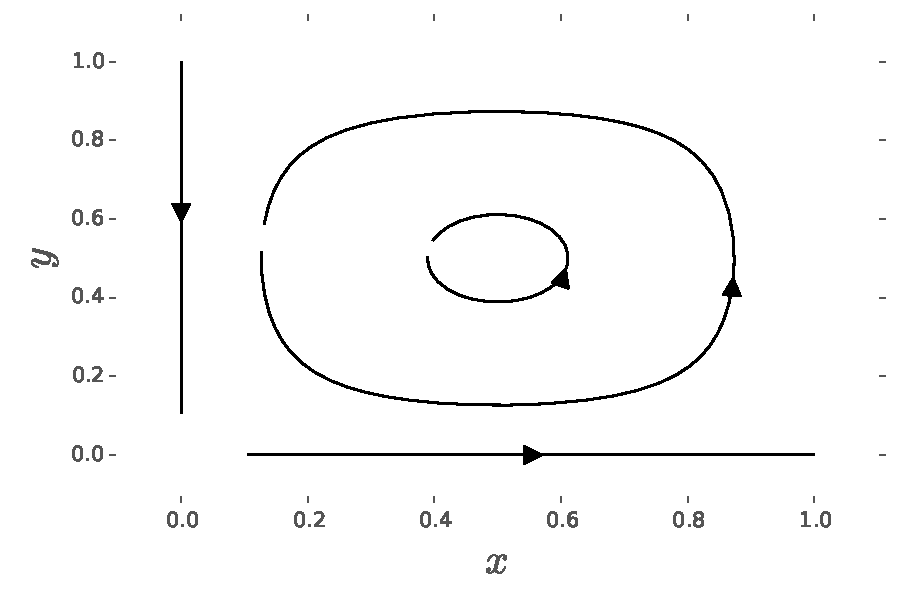
\includegraphics{skyrms-plot.pdf}
	\label{MP-phase}
	\caption{Phase diagram of replicator dynamics for matching pennies}
\end{figure}

In what follows we will largely use numerical simulations to explore the behavior of more complicated systems, but with reference to the concepts we have introduced in this section. This will allow us to explore more and more complicated systems.

%http://math.stackexchange.com/questions/761009/marginal-stability-and-centers-of-nonlinear-dynamical-systems

%http://www.theory.physics.manchester.ac.uk/~galla/lecture_notes_matching_pennies.pdf

%http://www.scholarpedia.org/article/Equilibrium#Types_of_Equilibria

\section{Signaling games}
\label{Signaling}

Now that we have outlined both the static and dynamic tools used to understand behavior in games, we turn to the asymmetric sequential games of incomplete information, \emph{signaling games}, that we will use subsequently to understand both communication and language change. First, signaling games are introduced. The relevant structures and definitions are presented along with a canonical example. Second, we consider the solution concepts from the previous sections. This allows us to determine the existence and characteristics of equilibria. Finally, we consider how signaling evolves according to the replicator dynamics.

It should be noted that there are multiple traditions that have contributed to the development of signaling games. In the Economic tradition the work of \cite{harsanyi:1967,harsanyi:1968a,harsanyi:1968b} on games of incomplete information and Spence's \citeyearpar{spence:1973} model of job signaling have been central. In the Philosophical tradition, the work of \cite{lewis:1969} has been the most influential. His response to the Quinean skepticism that meaning could arise by convention has had the most direct impact on Linguistics. This account, however, rests on the assumption that speakers and hearers have perfectly-aligned interests.  This assumption will figure in the exposition of this section, mostly for the simplicity it affords us in the examples. In the next section we turn towards the consequences of loosening it.

Signaling games offer an intuitive model of communication between agents.  A signaling game consists of two players, a sender and a receiver. The sender has some private piece of information, $t \in T$, drawn according to some commonly known probability distribution, $\delta$. The piece  of information can be thought of as some fact about the state of the world. For example, we might think of it as information that the sender wants to convey to the receiver. The sender chooses a message, $m \in M$, to send to the receiver.   The receiver does not know what state of the world actually holds and must choose an action, $a \in A$, as an interpretation of the message sent. That is, the receiver is faced with the problem of inferring the state of the sender given the message.

The outcome of the game is determined by the state of the sender, the message sent, and the action taken by the receiver. The sender and the receiver have preferences over these outcomes, which are given by utility functions, $U_S$ and $U_R$ respectively, which map outcomes to real numbers: $U_S,U_R:T \times M \times A \rightarrow \mathbb{R}$. Note that the message sent can figure into the utility functions. For example, if one message is costlier than another, then the utility can be adjusted to reflect this. In what follows we will only consider costless or \emph{cheap talk} signaling where all message incur the same cost, and thus do not affect the structure of the utility functions.

As a simple example of a signaling game, consider the case where there are two states, two messages, and two actions: $T = \{t_0, t_1 \}$, $M = \{m_0, m_1 \}$, and $A = \{a_0, a_1 \}$. We can represent the structure of the game in \emph{extensive form} as in Figure \ref{SG1}. The uppermost node, labeled $\delta$, determines the likelihood of either of the two states occurring. The lines from the uppermost node represent one state or the other obtaining. The nodes labeled $S$ indicate the points in the game where the sender makes a decision regarding which message to send. The nodes labeled $R$ indicate the points where the receiver must make a decision regarding how to interpret the message. The dashed lines between receiver nodes indicates that the receiver is uncertain as to which state holds after hearing a given message. The nodes at the bottom represent the outcome and the players' preferences, as determined by the utility functions.

%{every tree node/.style={align=center,anchor=north}}
%[scale=1, level/.style={sibling distance=70mm/#1}] 

\begin{figure}[!ht]
\centering
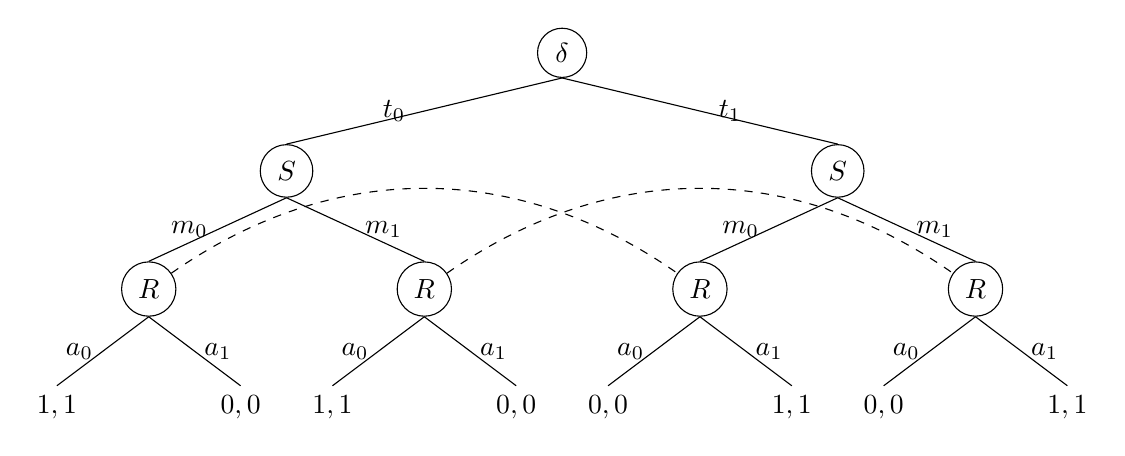
\begin{tikzpicture}[
	scale=1, level/.style={sibling distance=70mm/#1}]
\node  (z)[circle,draw]{$\delta$}
  child {node [circle,draw] (a_left) {$S$}
    child {node  [circle,draw](left_left) {$R$}
      child {node {$1,1$}        
      edge from parent
		node[left] {$a_0$}
		node[right] {}} 
      child {node (n){$0,0$}
      edge from parent
		node[left] {}
		node[right] {$a_1$}}
    edge from parent
	node[left] {$m_0$}
	node[right] {}}
    child {node  [circle,draw](left_right) {$R$}
      child {node {$1,1$}        
      edge from parent
		node[left] {$a_0$}
		node[right] {}} 
      child {node (n){$0,0$}
      edge from parent
		node[left] {}
		node[right] {$a_1$}}
    edge from parent
	node[left] {}
	node[right] {$m_1$}}
  edge from parent
	node[left] {$t_0$ $ $}
	node[right] {}
  }
 child {node [circle,draw] (a_right) {$S$}
    child {node  [circle,draw](right_left) {$R$}
      child {node {$0,0$}        
      edge from parent
		node[left] {$a_0$}
		node[right] {}} 
      child {node (n){$1,1$}
      edge from parent
		node[left] {}
		node[right] {$a_1$}}
    edge from parent
	node[left] {$m_0$}
	node[right] {}}
    child {node  [circle,draw](right_right) {$R$}
      child {node {$0,0$}        
      edge from parent
		node[left] {$a_0$}
		node[right] {}} 
      child {node (n){$1,1$}
      edge from parent
		node[left] {}
		node[right] {$a_1$}}
    edge from parent
	node[left] {}
	node[right] {$m_1$}}
  edge from parent
	node[left] {}
	node[right] {$ $ $t_1$}
  };
\draw [dashed](left_left) to [out=35,in=-215] (right_left);
\draw [dashed](left_right) to [out=35,in=-215] (right_right);
\end{tikzpicture}
\caption{Lewis signagling game with two states, two messages, and twos actions. }
\label{SG1}
\end{figure}

As alluded to above, with the exception of the topmost node and the leaves, all other nodes are \emph{decision nodes}. That is, they represent those points in the game where a particular player must make a decision. An \emph{information set} consists of a set of decision nodes for a given player, which that player cannot distinguish. For example, the receiver is in an information set after hearing $m_0$. She is not sure whether she is in the node beneath state $t_0$ or $t_1$ and she must choose between $a_0$ and $a_1$. She is likewise uncertain after receiving message $m_1$. Again, her inability to distinguish the two states is indicated by a dashed line. An information set can also consist of a single decision node. For example, the sender is never uncertain about the state he is in. Thus the information sets for the sender only ever consist of a single node. 

For each player, a \emph{strategy} specifies which action to take at all \emph{information sets} for a player.\footnote{For simplicity, we only consider \emph{pure} sender (receiver) strategies, functions from states to messages (messages to actions). \emph{Mixed} strategies are a straightforward generalization. A mixed sender strategy specifies a probability distribution over pure sender strategies, $\sigma = p_1 s_1 + ... + p_k s_k$, where $\sum_i p_i = 1$. Similarly, a mixed receiver strategy specifies a probability distribution over pure receiver strategies, $\rho = q_1 r_1 + ... + q_k r_k$.} We will refer to the set of all such sender strategies as $S : [T \rightarrow M ]$, and the set of all such receiver as $R : [M \rightarrow A]$. All pure sender and receiver strategies are summarized in Figure \ref{signaling-strategies}. The sender and receiver strategies that combine to yield a one-to-one mapping from states to actions are called \emph{signaling systems}. Thus, the strategy profiles $\langle s_1, r_1 \rangle$ and $\langle s_4, r_4 \rangle$ constitute signaling systems.

\begin{figure}
\begin{center}
\begin{tikzpicture}[->,>=stealth',shorten >=1pt,auto,node distance=2cm]
  \node (A)      {$t_0$};
  \node (B) [right=2cm of A]  {$m_0$};
  \node (C) [below of=A] {$t_1$};
  \node (D) [right=2cm of C] {$m_1$};
\path[->] (A) edge node {} (B)
	  (C) edge node {} (D);
   \node (name) [below left=.5cm and .5cm of A]  {$s_1:$};
   %
     \node (D) [right=3cm of B]   {$m_0$};
  \node (E) [right=2cm of D]  {$a_0$};
  \node (F) [below of=D] {$m_1$};
  \node (G) [right=2cm of F] {$a_1$};
\path[->] (D) edge node {} (E)
	  (F) edge node {} (G);
   \node (name) [below left=.5cm and .5cm of D]  {$r_1:$};
\end{tikzpicture}
\vspace{2cm}

\begin{tikzpicture}[->,>=stealth',shorten >=1pt,auto,node distance=2cm]
  \node (A)      {$t_0$};
  \node (B) [right=2cm of A]  {$m_0$};
  \node (C) [below of=A] {$t_1$};
  \node (D) [right=2cm of C] {$m_1$};
\path[->] (A) edge node {} (B)
	  (C) edge node {} (B);
   \node (name) [below left=.5cm and .5cm of A]  {$s_2:$};
   %
     \node (D) [right=3cm of B]   {$m_0$};
  \node (E) [right=2cm of D]  {$a_0$};
  \node (F) [below of=D] {$m_1$};
  \node (G) [right=2cm of F] {$a_1$};
\path[->] (D) edge node {} (E)
	  (F) edge node {} (E);
   \node (name) [below left=.5cm and .5cm of D]  {$r_2:$};
\end{tikzpicture}\\
\vspace{2cm}

\begin{tikzpicture}[->,>=stealth',shorten >=1pt,auto,node distance=2cm]
  \node (A)      {$t_0$};
  \node (B) [right=2cm of A]  {$m_0$};
  \node (C) [below of=A] {$t_1$};
  \node (D) [right=2cm of C] {$m_1$};
\path[->] (A) edge node {} (D)
	  (C) edge node {} (D);
   \node (name) [below left=.5cm and .5cm of A]  {$s_3:$};
   %
     \node (D) [right=3cm of B]   {$m_0$};
  \node (E) [right=2cm of D]  {$a_0$};
  \node (F) [below of=D] {$m_1$};
  \node (G) [right=2cm of F] {$a_1$};
\path[->] (D) edge node {} (G)
	  (F) edge node {} (G);
   \node (name) [below left=.5cm and .5cm of D]  {$r_3:$};
\end{tikzpicture}\\
\vspace{2cm}

\begin{tikzpicture}[->,>=stealth',shorten >=1pt,auto,node distance=2cm]
  \node (A)      {$t_0$};
  \node (B) [right=2cm of A]  {$m_0$};
  \node (C) [below of=A] {$t_1$};
  \node (D) [right=2cm of C] {$m_1$};
\path[->] (A) edge node {} (D)
	  (C) edge node {} (B);
   \node (name) [below left=.5cm and .5cm of A]  {$s_4:$};
   %
     \node (D) [right=3cm of B]   {$m_0$};
  \node (E) [right=2cm of D]  {$a_0$};
  \node (F) [below of=D] {$m_1$};
  \node (G) [right=2cm of F] {$a_1$};
\path[->] (D) edge node {} (G)
	  (F) edge node {} (E);
   \node (name) [below left=.5cm and .5cm of D]  {$r_4:$};
\end{tikzpicture}\\
\vspace{2cm}


\end{center}
\caption{Sender and Receiver strategies for signaling game}
\label{signaling-strategies}
\end{figure}



The set of possible combinations of sender and receiver strategies constitute \emph{strategy profiles}. That is, a sender strategy in the set of possible sender strategies, $s \in S$, and a receiver strategy in the set of all possible receiver strategies, $r  \in R$, yield a strategy profile $\langle s,r \rangle$. Each strategy profile determines the outcome of the game. Crucially, each player's utility function depends on the state of the sender and the action taken by the receiver. That is, their respective utilities are a function of state and action. As an example, consider the case where both sender and receiver prefer successful communication. Then they both receive their preferred payoffs if there is some correspondence between the sender's state and the receiver's action. For example, in Figure \ref{SG1} both sender and receiver prefer the state and action to be the same in the following sense.

\begin{equation}
 U_{S}(t_i, a_k) = U_{R}(t_i, a_k) =
\left\{
	\begin{array}{ll}
		1  & \mbox{if } i = k \\
		0 & \mbox{else}
	\end{array}
\right.
\end{equation}
Note that this reflects the assumption that both sender and receiver have the same preference over outcomes.

Given that the different states occur with certain probabilities, and we are interested in how particular strategies do on average, we consider the expected utility for a given strategy profile. This is simply the expected value of the utility functions given the two strategies, which can be given in the case of a discrete state space as in our example above.

\begin{equation}
\begin{split}
 E[U_{S}(s,r)] &= \sum_{t} \delta (t) \cdot U_S(t, r(s(t)))\\
 E[U_{R}(s,r)] &= \sum_{t} \delta (t) \cdot U_R(t, r(s(t)))
\end{split}
\end{equation}
For each possible state the sender and receiver strategies determine an outcome. $s(t)$ is the message the sender will employ and $r(s(t))$ is the action the receiver will take given that message. The expected utility is the sum of these outcomes weighted by the probability of the state that yields them. Assuming that the two states are equiprobable, we can construct the payoff matrix for the signaling game as in Table \ref{sig-table}. Since payoffs are symmetric, only one number is presented.

\begin{table}\centering
\begin{tabular}{lllll}
\hline\noalign{\smallskip}
 & $r_1$ & $r_2$ & $r_3$ & $r_4$ \\
\noalign{\smallskip}\hline\noalign{\smallskip}
$s_1$ & $1$ & $\frac{1}{2}$  & $\frac{1}{2}$  & $0$ \\

$s_2$ & $\frac{1}{2}$ & $\frac{1}{2}$  & $\frac{1}{2}$  & $\frac{1}{2}$ \\

$s_3$ & $\frac{1}{2}$ & $\frac{1}{2}$  & $\frac{1}{2}$  & $\frac{1}{2}$ \\

$s_4$ & $0$ & $\frac{1}{2}$  & $\frac{1}{2}$  & $1$ \\

\noalign{\smallskip}\hline
\end{tabular}
\caption{Payoff matrix for signaling game}
\label{sig-table}
\end{table}
There are several Nash equilibria in the game, but only the signaling systems $\langle s_1, r_1 \rangle$ and $\langle s_4, r_4 \rangle$  are evolutionarily stable strategies, because they are the only strict Nash equilibria. In fact, given the structure of the payoffs it is possible to show that these signaling systems are the unique asymptotically stable rest points of the system, which attract the entire interior of the state space \citep[82]{hofbauer-sigmund:1998}. This means that one of the two signaling systems is almost guaranteed to evolve.


%\begin{definition}
% A strategy profile $\langle s^*, r^*\rangle$ is a \emph{Nash equilibrium}
%if and only if:
%  \begin{itemize}
%   \item For all $s \in S$, such that $s \neq s^*$, $E[U_S(s^*,r^*)] \geq
%E[U_S(s,r^*)]$
%  \item For all $r \in R$, such that $r \neq r^*$, $E[U_R(s^*,r^*)] \geq
%E[U_S(s^*,r)]$
%  \end{itemize}
%\end{definition}

%Before I prove the theorems stated in the main text, I will first prove two lemmata that will be used frequently below.
%
%Lemma 10. Let ? be a partnership game with  payoff matrix A. Then:
%
%1.	
% is evolutionarily stable if and only if  is asymptotically stable under the replicator dynamics (1) generated by A.
%2.	
%The replicator dynamics (1) for \Gamma is a Shashshahani gradient system with potential function  .
%Proof. See Hofbauer and Sigmund (1998) p.82. ?
%
%The second part of Lemma 10 implies that all solutions converge to a rest point (Akin and Hofbauer 1982). Moreover, it implies that there are no circling solutions since the average payoff V is strictly increasing along all nonstationary solutions.

\section{The behavioral dynamics of signaling}

While the simplest signaling game can be analyzed in a fairly straightforward manner, we might be interested in larger, more complicated games. For example, we might wonder about the dynamics of signaling if the state space were continuous rather than discrete. If we were to approach this by first enumerating all sender and receiver strategies, the dimensions of the system would explode exponentially. One means of controlling for this increase suggested by \cite{hofbauer-huttegger2015} is to consider behavioral strategies insofar as no information is lost in doing so (cf. \citealt{kuhn1953}).\footnote{Erol Ak\c{c}ay (p.c.) has suggested a similar approach to the problem.} The basic idea is that instead of there being a single sender population and a single receiver population, there are multiple sender and receiver populations. Each sender population corresponds to a particular state, and messages compete to be used in that state. Each receiver population corresponds to a message, and actions compete to be used in response to that message.  We start off by defining the components necessary for our analysis. Once we have defined these components we can simulate the game dynamics.


%\begin{itemize}
%	\item The relationship between mixed strategies and behavioral strategies in extensive games of perfect recall is well understood \cite{kuhn1953}. In particular, if one is interested in the equilibrium structure of extensive form games, then no essential information is lost by focusing on behavioral strategies. We propose a similar move for the evolutionary dynamics of signaling games
%%	\item The selection-mutation dynamics in behavioral strategies can be thought of as a dynamics in the entries of the sender and receiver matrices, since these matrices are nothing but a representation of the game�s behavioral strategies.
%	\item A non-injective surjective function: a surjection
%	\item Lose information, condense
%\end{itemize}



%First, we define the payoff matrices for senders and receivers, which depend solely on the utility functions of senders and receivers respectively. $\textbf{A}$ is an $n \times n$ matrix such that $\textbf{A}_{ij} = U_S(t_i, a_j)$:
%
%
%\begin{equation}
%\textbf{A} =
% \begin{pmatrix}
%  U_S(t_1, a_1) & \cdots & U_S(t_1, a_j) & \cdots & U_S(t_1, a_n) \\
%  \vdots	        & \ddots & \vdots           &           & \vdots \\
%  U_S(t_i, a_1) & \cdots & U_S(t_i, a_j) & \cdots & U_S(t_i, a_n) \\  
%  \vdots	        &  & \vdots           &   \ddots        & \vdots \\
%  U_S(t_n, a_1) & \cdots & U_S(t_n, a_j)  & \cdots & U_S(t_n, a_n) \\
% \end{pmatrix}
%\end{equation}
%$\textbf{B}$ is an $n \times n$ matrix such that $\textbf{B}_{ij} = U_R(t_i, a_j)$:
%
%\begin{equation}
%\textbf{B} =
% \begin{pmatrix}
%  U_R(t_1, a_1) & \cdots & U_R(t_1, a_j) & \cdots & U_R(t_1, a_n) \\
%  \vdots	        & \ddots & \vdots           &           & \vdots \\
%  U_R(t_i, a_1) & \cdots & U_R(t_i, a_j) & \cdots & U_R(t_i, a_n) \\  
%  \vdots	        &  & \vdots           &   \ddots        & \vdots \\
%  U_R(t_n, a_1) & \cdots & U_R(t_n, a_j)  & \cdots & U_R(t_n, a_n) \\
% \end{pmatrix}
%\end{equation}
%
%
%Second, we define the sender and receiver populations. $\textbf{X}$ is a stochastic population matrix such that the proportion of the population in $x_i$ using $m_j$ is $x_{ij}$, with $\sum_j x_{ij} = 1$.
%
%\begin{equation}
%\textbf{X} =
% \begin{pmatrix}
%  x_{11} &  x_{12} & x_{13} \\
%  \vdots        & \vdots & \vdots \\
%  x_{i1} &  x_{i2} & x_{i3} \\
%  \vdots	& \vdots    & \vdots \\
%  x_{n1} &  x_{n2} & x_{n3} \\
% \end{pmatrix}
%\end{equation}
% 
%Intuitively, each row corresponds to a given state. Each element in the row corresponds to the proportion of use in that population.  Each row sums to one because the proportion using the various  signals must sum to one.
% 
%$\textbf{Y}$ is a population matrix such that the proportion of the population in $y_i$ responding with action $a_j$ is $y_{ij}$, with $\sum_j y_{ij} = 1$.
%
%\begin{equation}
%\textbf{Y} =
% \begin{pmatrix}
%  y_{11} & \cdots & y_{1j}  & \cdots & y_{1n} \\
%  y_{21} & \cdots & y_{2j}  & \cdots & y_{2n} \\
%  y_{31} & \cdots & y_{3j}  & \cdots & y_{3n} \\
% \end{pmatrix}
%\end{equation}
%
%Again, intuitively, each row corresponds to a given message. Each element in the row corresponds to the proportion of different responses to the message. Each row sums to one because the proportion using the various responses must sum to one.
% 
% 
%The expected utility of sending message $m_j$ in state $t_i$, where $\textbf{Y}^T$ is the transpose of $\textbf{Y}$:
%
%\begin{equation}
%	E [ x_{ij} ] = (\textbf{A}\textbf{Y}^T)_{ij}
%\end{equation}
%
%The average expected utility in a sender population $x_i$:
%
%\begin{equation}
%	E [ x_{i} ] = (\textbf{X}(\textbf{A}\textbf{Y}^T)^T)_{ii}
%\end{equation}
%
%This gives the replicator dynamic for a given message in a sender population.
%\begin{equation}
%	\dot{x}_{ij} = x_{ij}((\textbf{A}\textbf{Y}^T)_{ij} - (\textbf{X}(\textbf{A}\textbf{Y}^T)^T)_{ii})
%\end{equation}
%
%
%
%
%$\textbf{P}$ is a stochastic matrix such that $\forall i \textbf{P}_i = P(t_1),...,P(t_n)$. That is, $\textbf{P}$ is just $n$ rows of the prior probability distribution over states.
%
%\begin{equation}
%\textbf{P} =
% \begin{pmatrix}
%  P(t_1) & \cdots & P(t_i)  & \cdots & P(t_n) \\
%  \vdots &  & \vdots  & & \vdots  \\
%  P(t_1) & \cdots & P(t_i)  & \cdots & P(t_n) \\
% \end{pmatrix}
%\end{equation}
%
%
%Now that we have defined the  replicator dynamics for the sender populations, we can do the same for the receiver populations with a few additions. Let $\textbf{C}$ be the conditional probability of a state given a message. That is, $\textbf{C}_{ij} = P(t_i | m_j)$, where $\otimes$ indicates element-wise Hadamard multiplication and $\oslash$ indicates the element-wise Hadamard division.
%
%\begin{equation}
%\textbf{C} = (P^T \otimes X) \oslash (PX)
%\end{equation}
%
%
%The expected utility of receiver responding to message $m_i$ with action $a_j$:
% 
%\begin{equation}
%	E [ y_{ij} ] = (\textbf{B}^T\textbf{C})_{ji}
%\end{equation}
%
%Since the resulting matrix is $n \times m$, we swap the indices to get the appropriate value. Each column corresponds to a receiver population, and each row corresponds to a response action.
%
%The average expected utility in a receiver population $y_i$:
%
%\begin{equation}
%	E [ y_{i} ] = (Y(\textbf{B}^T\textbf{C})_{ji})_{ii}
%\end{equation}
%
%The replicator dynamic for a given action in response to a message is given by the following.
%
%\begin{equation}
%		\dot{y}_{ij} = y_{ij}(\textbf{B}^T\textbf{C})_{ji} - (Y(\textbf{B}^T\textbf{C})_{ji})_{ii})
%\end{equation}
%Together these behavioral replicator dynamics can be used to investigate any signaling game with a finite number of states, messages, and actions.

\subsection{The simplest signaling game}

To begin, we apply this new framework to the simplest non-trivial signaling game where we have two equiprobable states, two messages, and two actions. The structure of the behavioral  replicator dynamics is determined by the structure in Figure \ref{behavioral-dynamics}. $x_0$ represents the probability that $m_0$ will be used in the $t_0$ sender population. Likewise $x_1$ represents the probability that $m_1$ will be used in the $t_1$ sender population. The dotted lines indicates probabilities that can be derived from others. All told, then, the behavioral replicator dynamic  for this signaling game gives rise to a four-dimensional system.

\begin{figure}
\begin{center}
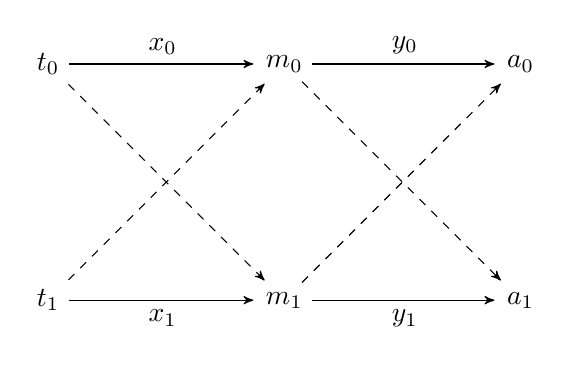
\begin{tikzpicture}[->,>=stealth',shorten >=1pt,auto,node distance=3cm]
  \node (A)      {$t_0$};
  \node (B) [right of=A]  {$m_0$};
  \node (C) [right of=B] {$a_0$};
  \node (D) [below of=A] {$t_1$};
  \node (E) [right of=D] {$m_1$};
  \node (F) [right of=E] {$a_1$};
\path[->] (A) edge node {$x_0$} (B)
	  (A) edge[dashed,pos=0.85] node {} (E)
	  (B) edge node {$y_0$} (C)
	  (B) edge[dashed,pos=0.85] node {} (F)
	  (D) edge[below] node {$x_1$} (E)
	  (D) edge[dashed,pos=0.75] node {} (B)
	  (E) edge[below] node {$y_1$} (F)
	  (E) edge[dashed,pos=0.75] node {} (C);
\end{tikzpicture}
\end{center}
\caption{Signaling game in behavioral space}
\label{behavioral-dynamics}
\end{figure}

We will generalize the parameters a bit to match the simpler games we used above. Namely, let the sender and receiver payoffs be the following matrices, with parameters $\alpha$ and $\beta$.

\begin{equation}
\mathbf{A} =
 \begin{pmatrix}
  1 - \alpha & \alpha \\
  \beta & 1 - \beta \\
 \end{pmatrix}
\end{equation}

\begin{equation}
\mathbf{B} =
 \begin{pmatrix}
  1 & 0 \\
  0 & 1 \\
 \end{pmatrix}
\end{equation}
These yield the general behavioral sender and receiver replicator dynamics.

\begin{equation}
	\begin{split}
		\dot{x}_0 &= x_0(1-x_0)(y_0 + y_1 - 1)(1 - 2\alpha)\\	
		\dot{x}_1 &= x_1(1-x_1)(y_0 + y_1 - 1)(1 - 2\beta)\\
	\end{split}
\end{equation}

\begin{equation}
	\begin{split}
		\dot{y}_0 &= y_0(1 - y_0)\left(\frac{x_0 + x_1 - 1}{x_0 - x_1 + 1}\right)\\
		\dot{y}_1 &= y_1(1 - y_1)\left(\frac{x_0 + x_1 - 1}{x_1 - x_0 + 1} \right)\\
	\end{split}
\end{equation}

 The case where $\alpha = \beta = 0$ corresponds to the lewis signaling game we introduced in the previous section, which is also related to the coordination game we started with. This is a signaling games with common interests. The case where $\alpha = \beta = 1$ corresponds to signaling with matching pennies. This is a signaling game with conflicting interests.  The cases where $\alpha = 0, \beta = 1$  and $\alpha = 1, \beta = 0$ also offer an interesting comparison. These are games of at least partial common interest. We address each of these below.

\subsection{Signaling under common interests}

Since the receiver dynamics do not vary as we change the parameters, we omit them. Under common interests the sender dynamics are the following.

\begin{equation}
	\begin{split}
		\dot{x}_0 &= x_0(1-x_0)(y_0 + y_1 - 1)\\	
		\dot{x}_1 &= x_1(1-x_1)(y_0 + y_1 - 1)\\
	\end{split}
\end{equation}

Typical results for a numerical solution are shown in Figure \ref{common-interests}, where we plot $x_0$ against $y_0$ and $x_1$ against $y_1$, with circles represent the starting state of both of trajectories. That is, we represent the four-dimensional system as two two-dimensional systems overlaid on each other. The established result is exactly what we see. Namely, the system either converges to the origin or to the upper right-hand corner. Referring back to Figure \ref{behavioral-dynamics} it is clear that these constitute the signaling systems of the signaling game as we described them. That is, these are the points that guarantee a one-to-one mapping between states and actions.


\begin{figure}
	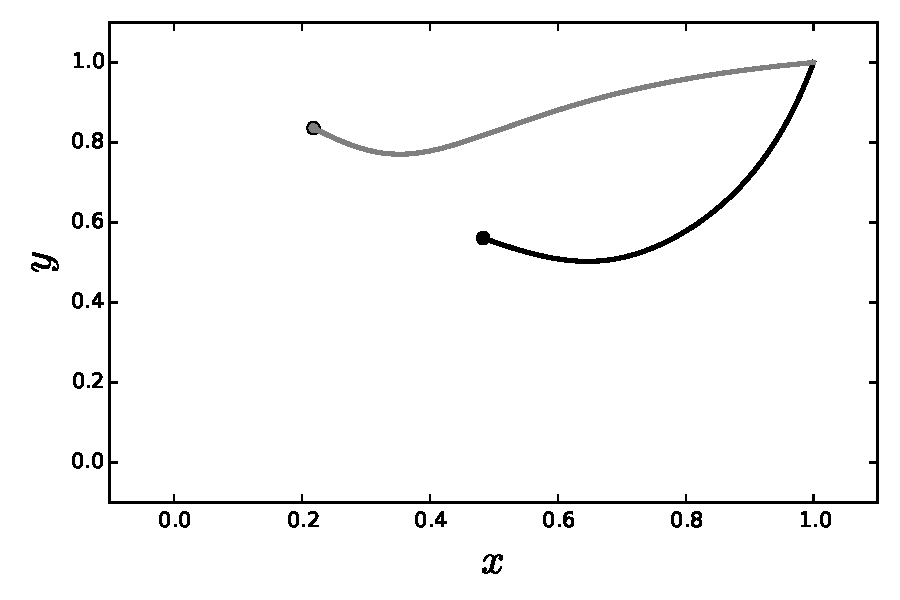
\includegraphics{common-interests.pdf}
	\label{common-interests}
	\caption{Solution trajectories for behavioral replicator dynamics for common interest signaling}
\end{figure}


%\begin{equation}
%	\mathbf{J} 
%	 =
%	 \begin{bmatrix} 
%	(- 2 x_{0} + 1) (y_{0} + y_{1} - 1) & 0 & x_{0} (- x_{0} + 1) & x_{0} (- x_{0} + 1)\\
%	0 & (- 2 x_{1} + 1) (y_{0} + y_{1} - 1) & x_{1} (- x_{1} + 1) & x_{1} (- x_{1} + 1)\\
%	\frac{2 y_{0} (x_{1} - 1) (y_{0} - 1)}{(x_{0} - x_{1} + 1)^{2}} & - \frac{2 x_{0} y_{0} (y_{0} - 1)}{(x_{0} - x_{1} + 1)^{2}} & \frac{(- 2 y_{0} + 1) (x_{0} + x_{1} - 1)}{x_{0} - x_{1} + 1} & 0 \\
%	- \frac{2 x_{1} y_{1} (y_{1} - 1)}{(- x_{0} + x_{1} + 1)^{2}} & \frac{2 y_{1} (x_{0} - 1) (y_{1} - 1)}{(- x_{0} + x_{1} + 1)^{2}} & 0 & \frac{(- 2 y_{1} + 1) (x_{0} + x_{1} - 1)}{- x_{0} + x_{1} + 1}\\
%	 \end{bmatrix}
%\end{equation}
%
%It's clear that both $\frac{\partial \dot{y}_0}{\partial x_0}$ and $\frac{\partial \dot{y}_1}{\partial x_0}$ go to infinity as we approach points at the edge of the state space.

%\begin{figure}
%	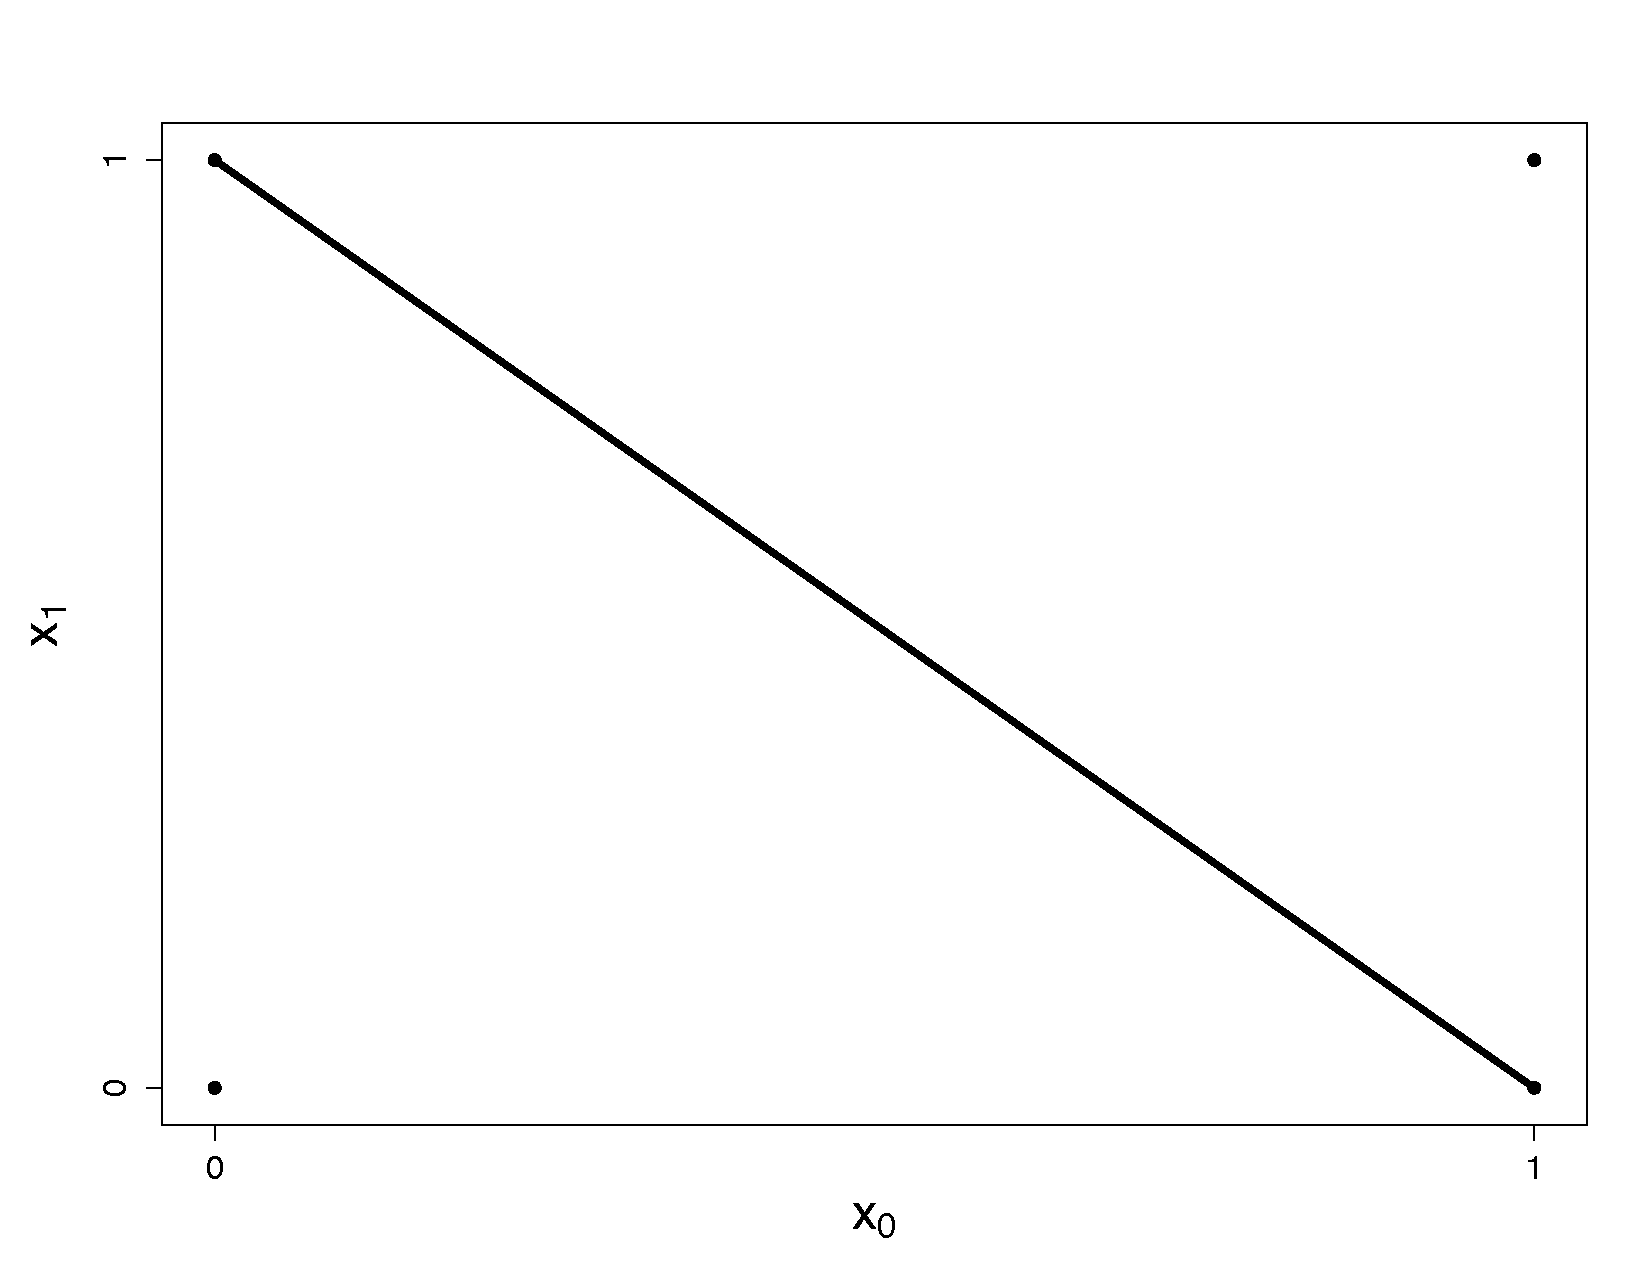
\includegraphics[width=.5\textwidth]{lewis-phase-portrait-senders}	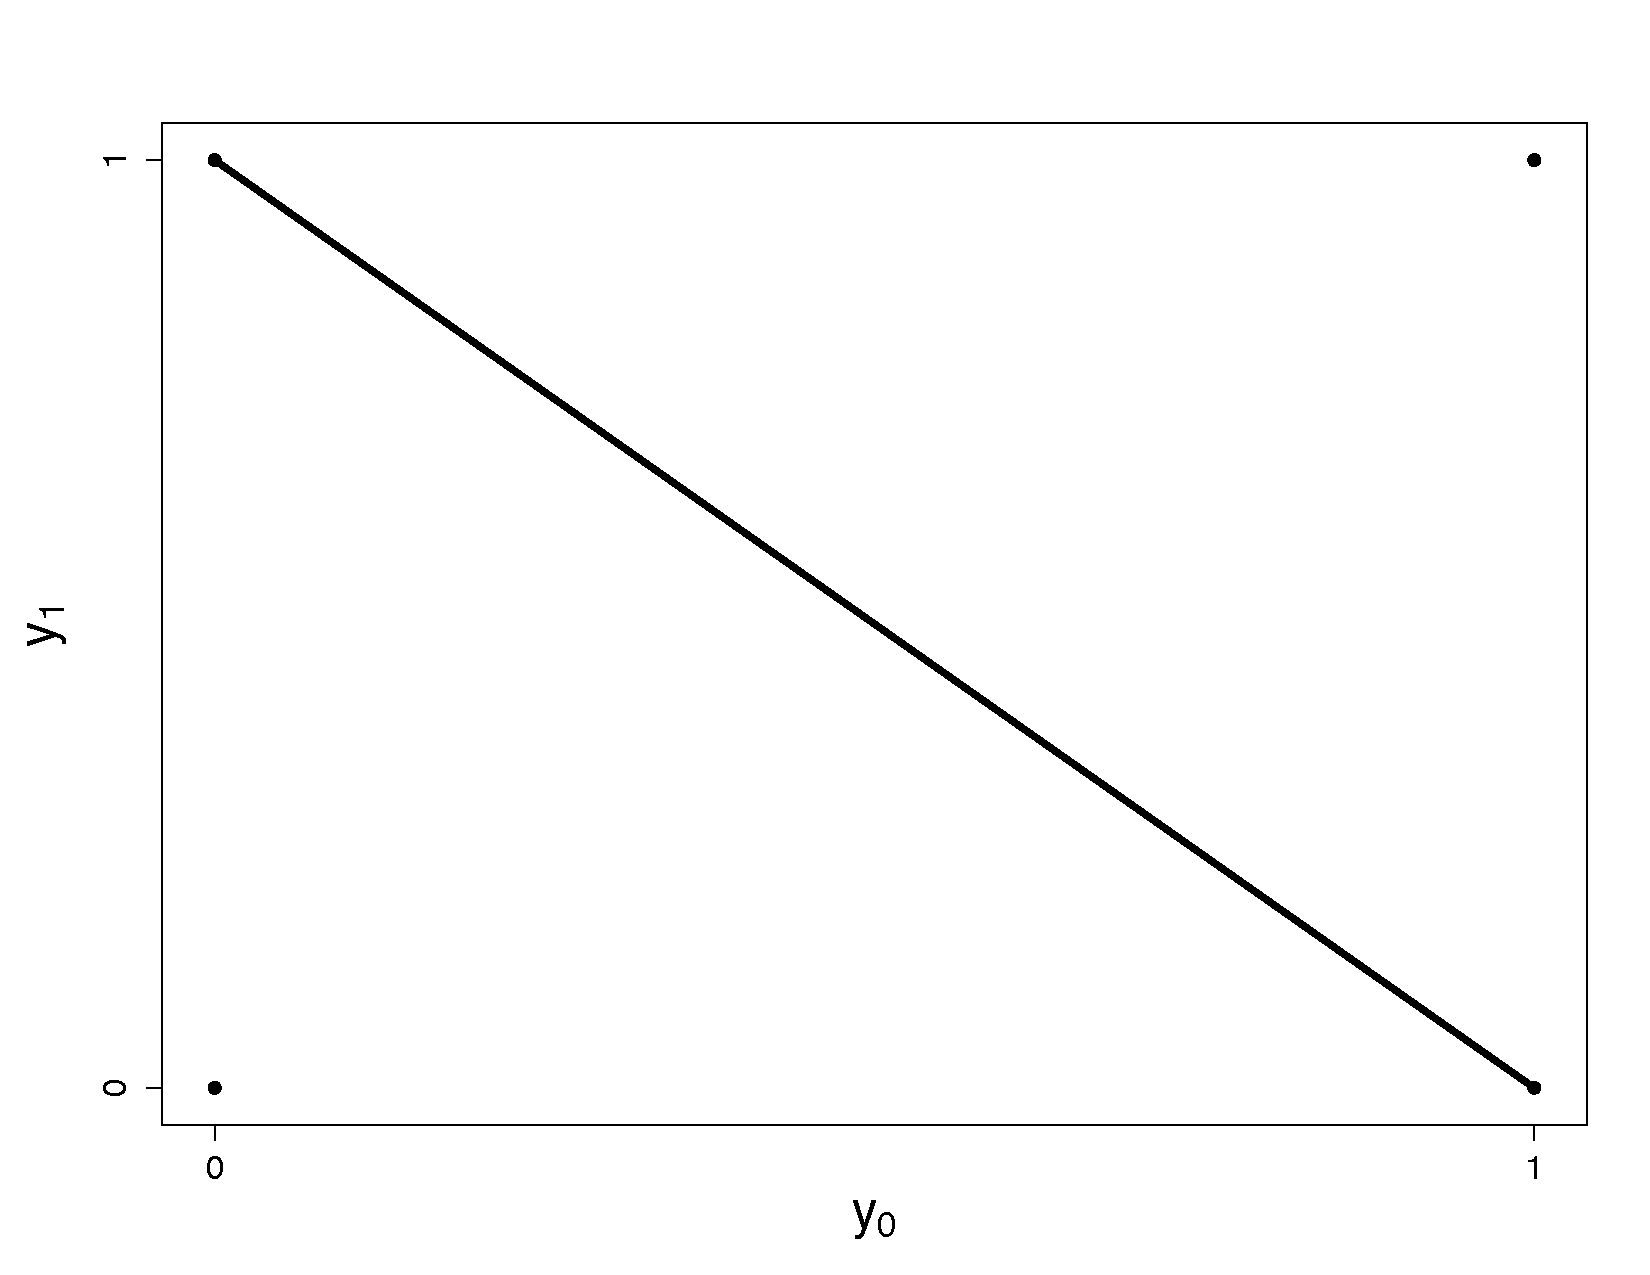
\includegraphics[width=.5\textwidth]{lewis-phase-portrait-receivers}		
%\end{figure}


\subsection{Signaling under conflicting interests}

If we alter the payoff structure to reflect that of matching pennies, then the following behavioral sender dynamics result.
\begin{equation}
	\begin{split}
		\dot{x}_0 &= x_0(1-x_0)(1 - y_0 - y_1)\\	
		\dot{x}_1 &= x_1(1-x_1)(1 - y_0 - y_1)\\
	\end{split}
\end{equation}

Typical results for numerical solution are shown in Figure \ref{conflicting-interests}. Interestingly, much like in the case of matching pennies, the system exhibits closed orbits.

\begin{figure}
	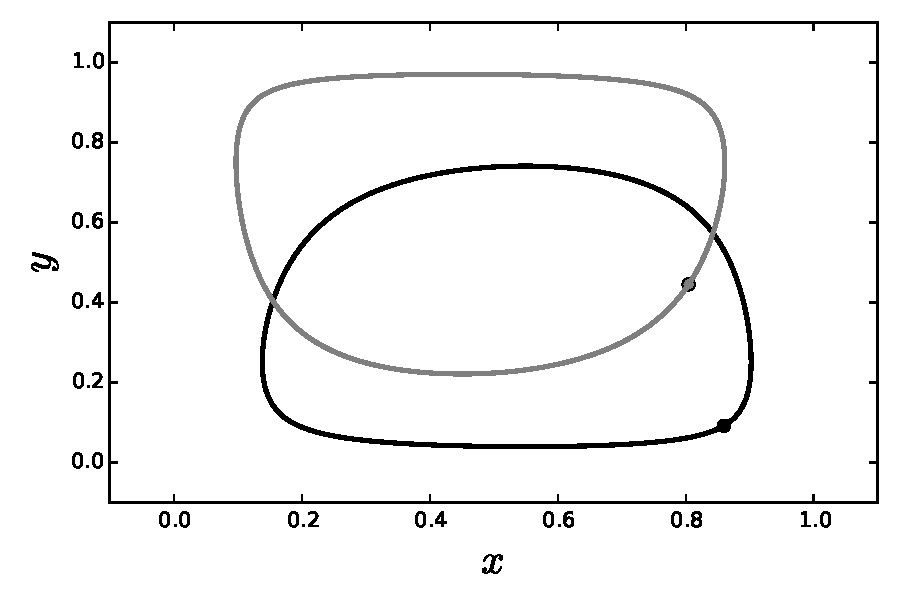
\includegraphics{conflicting-interests.pdf}
	\label{conflicting-interests}
	\caption{Solution trajectories for behavioral replicator dynamics for conflicting interest signaling}
\end{figure}

An interesting consequence of this behavior is that despite the fact that the sender does not want to signal what action he is going to take, there is some amount of information carried by the signal. This can quantified by calculating the \emph{Kullback-Leibler divergence} or \emph{information gain} due to the signal.

\begin{equation}
	KL(m) = \sum_t P(t \mid m) log \left( \frac{P(t \mid m)}{P(t)} \right)
\end{equation}
The basic intuition behind this formula is that it allows us a way to compare the receiver's expectations prior to receiving the message, which is determined by the probability distribution over states, to the posterior distribution after having heard the message.  The difference between these two distributions is the information gained by having received the message. The average information gain for the two signals is shown in Figure \ref{conflicting-interests-KL}. As a point of reference, if the messages perfectly corresponded to states, as they do in a signaling system, then the average information gain would be equal to one. In other terms, the information gained from the signal would be one bit, because it would allow us to distinguish between two equiprobable states. The fact that signals still carry information, even under diametrically opposed interests is both interesting and surprising (cf. \citealt{sato-etal2002,wagner2012}).


\begin{figure}
	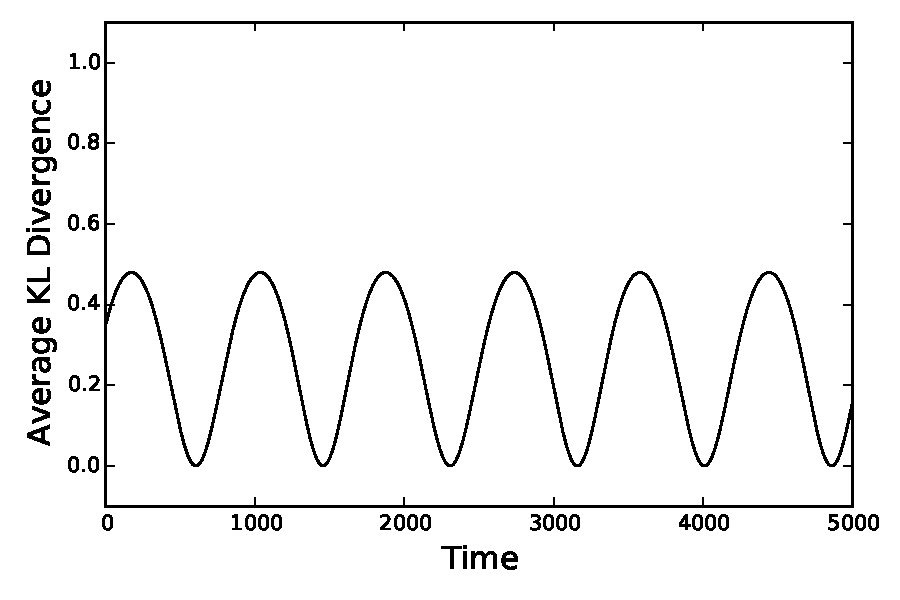
\includegraphics{conflicting-interests-KL.pdf}
	\label{conflicting-interests-KL}
	\caption{Average Kullback-Leibler Divergence for signals under conflicting interests}
\end{figure}


%\subsection{Partial Common Interests}
%
%Perhaps even more surprising is the case of only partially misaligned interests, or as \cite{blume-etal:2001} refer to them, \emph{partial common interests}. That is, when $\alpha = 0, \beta = 1$  and $\alpha = 1, \beta = 0$, then at least some of the time senders want to accurately signal their type. Consider the case where $\alpha = 1, \beta = 0$, which yields the following behavioral dynamics.
%
%\begin{equation}
%	\begin{split}
%		\dot{x}_0 &= x_0(1-x_0)(1 - y_0 - y_1)\\	
%		\dot{x}_1 &= x_1(1-x_1)(y_0 + y_1 - 1)\\
%	\end{split}
%\end{equation}
%
%\begin{figure}
%	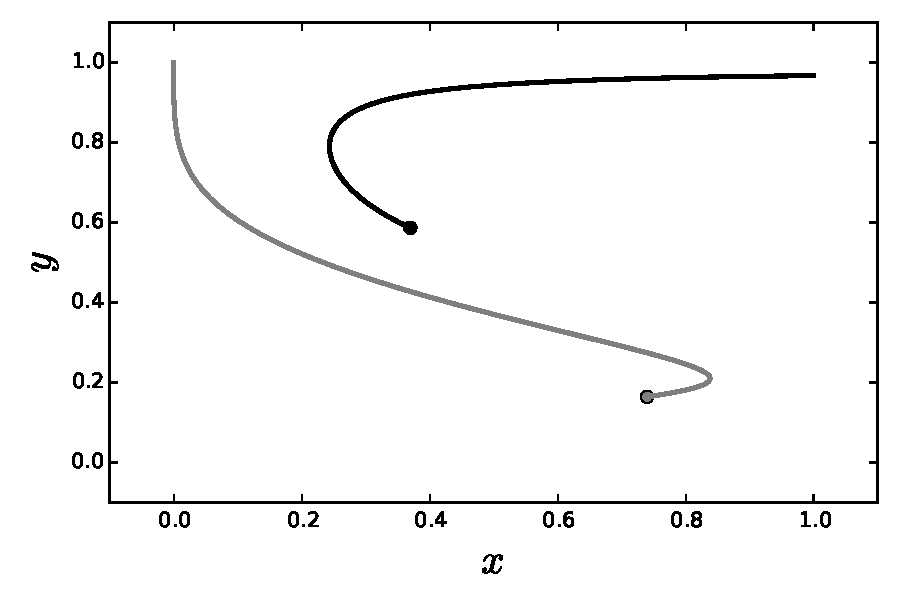
\includegraphics{partial-common-interests.pdf}
%	\label{partial-common-interests}
%	\caption{Solution trajectories for behavioral replicator dynamics for partial common interest signaling}
%\end{figure}
%
%Typical results for a numerical solution are presented in Figure \ref{partial-common-interests}. The sender populations converge to opposite sides of the state space, meaning that senders all converge on using the same signal. In response to this, receivers converge to some intermediate response, although not necessarily the one that might be expected from the distribution over states. The most striking thing about this case is that it differs dramatically from the case where interests are perfectly opposed. In the first case no information is carried by the messages, whereas there is always some information carried by messages in the second.


\section*{Summary}

In this chapter we outlined the basic framework that will be used subsequently. We noted the complementary role of static and dynamic methods for understanding the evolution of populations. We also presented a general method for describing the dynamics of signaling games and noted interesting properties of the simplest kind of signaling game. We now turn to our application of this framework to the functional cycle.


%\chapter{Evolutionary Game Theory (20 pages)}
%\label{evolutionary-game-theory}
%
%\section{Games}
%\label{Games}
%
%Game theory is a branch of applied mathematics that models human decision-making when the outcomes and preferences of multiple agents are intertwined. This differs from decision theory, where a single agent is faced with bringing about his or her most preferred outcome. Rather, a game arises when the choices made by each player crucially depend on those made by others. For example, when driving a car, one prefers to be on the opposite side of the road as the next oncoming vehicle. The side of the road that best achieves the outcome of not crashing is irrelevant, but it depends on how everyone involved drives.
%
%There are two general dimensions along which the structures of games vary. The first dimension is the order in which players make their decisions. If all players make a decision at the same time, then the game is a \emph{simultaneous} game. If players make their decisions in a particular order, then the game is a \emph{sequential} game. The second dimension is the knowledge the players have of the game. If all players know all of the 
%
%\begin{itemize}
%	\item Complete
%	\item Perfect
%	\item Incomplete
%	\item Tadelis
%\end{itemize}
%
%\begin{itemize}
%	\item Coordination
%	\item Trust Game
%\end{itemize}
%
%\begin{table}\centering
%\begin{tabular}{lll}
%\hline\noalign{\smallskip}
% & A & B \\
%\noalign{\smallskip}\hline\noalign{\smallskip}
%A & $1$ & $0$ \\
%B & $0$ & $1$ \\
%\noalign{\smallskip}\hline
%\end{tabular}
%\caption{Prisoner's Dilemma}
%\label{PD}
%\end{table}
%
%
%Trust Games are sequential games that allow for cooperation. They consist of an
%agent who has the option to invest some proportion of an endowment with a
%trustee whom they do not know and will not meet. The amount invested grows by some
%positive rate and the trustee then decides what proportion, if any, to return to
%the investor. Suppose we let $e$ be the initial endowment and $r > 1$ be the
%rate of growth. Further, let us give the investor the option of investing the
%entire endowment or none of it.  Finally, let us give the trustee the option of
%returning some proportion $p > 0$ of the resulting amount, or none of it.  We
%can represent this game in extensive form as in Figure \ref{tg}.
%
%\begin{figure}[ht]
%\begin{center}
%\begin{tikzpicture}[level/.style={sibling distance=50mm}]
%\node [circle, draw] (z){$X$}
%  child {node  {$(e,0)$}
%%     child {node  (b) {(1,1)}
%% 	}
%%     child {node  (g) {(0,0)}
%%    }
%  edge from parent
%	node[left] {$0$}
%	node[right] {}
%  }
%  child {node [circle,draw] (j) {$Y$}
%    child {node  (k) {$(0,re)$}      
%    edge from parent
%					node[left] {$0$}
%					node[right] {}}
%  child {node (l) {$(pre,(1-p)re)$}
%	edge from parent
%	      node[left] {}
%	      node[right] {$p$}
%  }edge from parent
%	node[left] {}
%	node[right] {$e$}
%};
%\end{tikzpicture}
%\caption{\textbf{Trust Game:} The investor, $X$, can invest all or none of an
%endowment. The amount invested grows by $r$.  The Trustee, $Y$, can then return
%some proportion of the resulting amount, or none of it.}
%\label{tg}
%\end{center}
%\end{figure}
%
%It is only worthwhile for the investor to make an investment if the amount
%returned is greater than the initial investment.  That is, if there
%is some profit to be made by investing at all.  If the Trustee always returned
%some amount, it would suffice for $pr > 1$ for this to be true. However,
%it is always best for the trustee to keep any amount that is invested, given
%that keeping all of the resulting amount is better than keeping only some of
%it: $re > (1-p)re$, given that $p > 0$.  Knowing that the Trustee has no
%incentive to return any of the amount invested, the Investor should never invest
%anything, because it will never yield a profit.  Both could do better if some
%amount were invested and returned, but neither investing nor returning any
%amount is rational. To achieve this outcome, where both Investor and Trustee are
%better off, requires that the Investor trust the Trustee to
%cooperate.
%
%
%\section{Equilibria}
%
%A game by itself does not constitute a model in the technical sense. It is a mathematical structure that describes the players preferences and actions, but it does not predict their behavior \emph{per se}. To do so it must be supplemented with a \emph{solution concept} that predicts the conditions under which particular outcomes will obtain. Perhaps the most widely used solution concept is that of a \emph{Nash equilibrium}, which specifies when players have an incentive to unilaterally deviate from a given strategy profile.
%
%\begin{definition}
% A strategy profile $\langle s^*, r^*\rangle$ is a \emph{Nash equilibrium}
%if and only if:
%  \begin{itemize}
%   \item For all $s \in S$, such that $s \neq s^*$, $E[U_S(s^*,r^*)] \geq
%E[U_S(s,r^*)]$
%  \item For all $r \in R$, such that $r \neq r^*$, $E[U_R(s^*,r^*)] \geq
%E[U_S(s^*,r)]$
%  \end{itemize}
%\end{definition}
%
%The two conditions simply state that neither the sender nor the receiver can do better by individually changing his or her strategy from the equilibrium profile.  The sender's strategy is his \emph{best response} to the receiver's strategy, and the receiver's strategy is likewise her best response to the sender's strategy. Note that these best responses need not be unique to consitute an equilibrium. This follows from the fact that the inequalities in the definiton are not strict. We can, however, impose uniqueness in these best responses by requiring that the inequalities in the definition be strict. A \emph{strict Nash equilibrium} results, meaning that players can only ever do worse if they unilaterally deviate from the equilibrium. Strict Nash equilibria are thus a proper subset of Nash equilibria.
%
%Since we are interested not just in the behavior of a given sender and receiver, but rather the aggregate behavior of a population, we want a broader notion of equilibrium. In particular, we might ask whether a given population is susceptible to change. When considering \emph{asymmetric games}, such as signaling games, where players have different roles, we are actually concerned with two populations: a sender population and a receiver population. To determine the stability of the two populations we can consider a \emph{symmetrized} version of the signaling game, where individuals act as both sender and receiver. A strategy in the symmetrized game is thus a strategy profile of the asymmetric game.
%
%In the case of the static problem, stability is determined with reference to static solution concepts. At the population level, the most relevant concept is that of an \emph{evolutionarily stable strategy} \citep{maynard-smith-price:1973,maynard-smith1982}. Where $U(S^*, S)$ is the payoff to an agent using strategy $S^*$ against an agent using strategy $S$, we have the following definition.
%
%\begin{definition}
% A strategy $S^*$ is an evolutionarily stable strategy (ESS) if and only if, for all alternate strategies $S$:
%\begin{enumerate}
% \item $U(S^*, S^*) \geq U(S,S^*)$
% \item If $U(S^*, S^*) = U(S,S^*)$ then $U(S^*, S) > U(S,S)$
%\end{enumerate}
%\end{definition}
%
%A straightforward interpretation of this definition can be had by imagining a population composed entirely of individuals playing $S^*$. Suppose some small proportion, $1 \gg \epsilon > 0$, of individuals playing the alternative $S$ is introduced into the population. The following inequality holds if and only if $S^*$ is an ESS.
%
%\begin{equation}
%\label{ESSlinear}
%(1-\epsilon )U(S^*,S^*) + \epsilon U(S^*,S)  > (1-\epsilon)U(S,S^*) + \epsilon U(S,S)
%\end{equation}
%In other words, for any sufficiently small influx of the alternate strategy, the expected payoff of the incumbent strategy in the resulting population is strictly greater than that of the alternate. Intuitively, $S^*$ is stable because selection will carry the population back to playing $S^*$.
%
%It is important to note, despite the dynamic terminology, an ESS is still an essentially static concept. We may naturally expect some form of selection to eliminate strategies with lower expected payoffs and carry the population back to playing $S^*$. But, we have not been explicit about the game dynamic that does the carrying. \cite{taylor-jonker:1978} introduced the replicator dynamic to explicitly address the dynamical aspects of evolutionarily stable strategies. Thus there is a fundamental connection between the two. This connection does not necessarily extend to other game dynamics though. There is no guarantee that solutions to the static problem will tell us anything about solutions to the dynamic problem for game dynamics in general. What we need is a set of criteria that can be applied to any game dynamic.
%
%
%For a population playing the symmetrized game, change depends on whether a given strategy is an \emph{evolutionarily stable strategy} \citep{maynard-smith-price:1973}. Loosely speaking, a strategy is evolutionarily stable if it is resistant to invasion by alternate strategies. That is, when an entire population plays the incumbent strategy the incumbents do at least as well as a mutant. If the mutant does as well, then the incumbent strategy should do better than a mutant in an all-mutant population.  In this case a mutation can be interpreted either in the biological sense or in terms of cultural innovation, such as the introduction of new linguistic signal. The relevant criterion for stability is actually quite simple. For symmetrized asymmetric games, a strategy profile is  evolutionarily stable if and only if it constitutes a strict Nash equilibrium in the original asymmetric game \citep{selten:1980}. That is, mutant senders and receivers only ever do worse than the incumbent strategies. 
%
%For the Lewisian signaling game described above, where states are equiprobable, $\delta(t_1) = \delta(t_2) = \frac{1}{2}$, the only strict equilibria are those where senders employ different signals for each state, and receivers map those messages to the appropriate actions. In other words, the senders \emph{separate} themselves and receivers respond accordingly. These equilibria are referred to as \emph{separating equilibria}. There are also equilibria where senders \emph{pool} themselves together and use only a single message. Receivers are indifferent between actions; they receive the same expected utility for taking either action. These are referred to as \emph{pooling equilibria}. Note that these pooling equilibria are not strict insofar as any action taken by the receiver yields the same expected utility. Thus, in the case of perfectly-aligned interests, separating equilibria are the only evolutionarily stable strategies.
%
%
%\section{Dynamics}
%
%While the term suggests a dynamic interpretation, equilibria, including evolutionarily stable strategies are essentially a static solution concept. They tell us whether a strategy is resistant to invasion or innovation, but tell us nothing about where the populations go to from there. To understand how a population changes over time, a particular \emph{game dynamics} must be supplied. These provide a  description for how a population, or populations, changes from one point in time to the next. Here we use the replicator equations as our game dynamic.
%
%Originally developed as a model of biological replication under selection \citep{taylor-jonker:1978}, the replicator equations are appealing for a number of reasons. First, they are the most extensively studied dynamics and share a number of mathematical properties with a larger set of game dynamics \citep{hofbauer-sigmund:1998}.  This makes establishing results and connecting them to a broader class of dynamics more straightforward. Second, they have a natural interpretation as a form of learning or cultural imitation \citep{fudenberg-levine:1998} and have found broad application in modeling economic \citep{samuelson:1997, cressman:2003} and social behavior \citep{skyrms:1996,skyrms:2004,skyrms:2010}.
%
%The intuition behind the replicator equations is that  more successful strategies increase in frequency. In particular, strategies that are more successful than the population average increase in share of the population. For example, let $\mathbf{x}$ and $\mathbf{y}$ represent the composition of a sender and receiver population respectively. $x_i$ represents the proportion of senders who use strategy $s_i$, and $y_i$ represents the proportion of receivers who use strategy $r_i$. The change of $x_i$ in the population, $\dot{x}_i$, can be given as the following where $f_i(\mathbf{y})$ is the expected utility of $s_i$ given the receiver population, and the average sender expected utility is given as $f(\mathbf{y}) = \sum_{i} x_if_i(\mathbf{y})$.
%
%\begin{equation}
%     \dot{x}_i = x_i(f_i(\mathbf{y}) - f(\mathbf{y}))
%\end{equation}
%The parallel formulation for receiver strategies is then the following, $g_i(\mathbf{x})$ is the expected utility of $r_i$ and $g(\mathbf{x}) = \sum_{i} y_ig_i(\mathbf{x})$.
%
%\begin{equation}
%     \dot{y}_i = y_i(g_i(\mathbf{x}) - g(\mathbf{x}))
%\end{equation}
%
%Sender and receiver strategies that do better than average have a positive derivative and thus increase. Sender and receiver strategies that do worse than average have a negative derivative and thus decrease. The \emph{rest points} of the dynamics are compositions of the respective populations that do not change from one point in time to the next. Note that by definition Nash equilibria constitute rest points of the dynamics. Neither senders nor receivers have an incentive to deviate from their respective equilibrium strategies. Thus, the average expected utility is identical to the expected utilities of the equilibrium strategies, and the composition of the population does not change.
%
%While we noted that the pooling equilibria in the game described above are not evolutionarily stable strategies, the game dynamics yield further information. That is, the pooling equilibria are saddle points of the dynamics. Almost any small deviation from them leads the population to converge to one of the separating equilibria, which are evolutionarily stable strategies. Crucially, any small difference in the response of receivers to the different signals allows for a kind of tie-breaking. Senders respond to the receivers differentiation by separating, and the population as a whole moves towards one of the separating equilibria.
%
%A bit more formally, for a state space $\mathbf{x} = \{x_1, x_2,...,x_n \}$, a solution trajectory through the state space over time $\mathbf{x(t)}$ is governed by the differential equations defined by the game dynamics $\mathbf{\dot{x}} = \{\dot{x}_1, \dot{x}_2,...,\dot{x}_n \}$. The rest points of the system are states where the differential equations vanish; any trajectory starting at a rest point will remain there at rest. For a rest point $\mathbf{x^*}$, if $\mathbf{x(0)} = \mathbf{x^*}$ then $\mathbf{x(t)} = \mathbf{x^*}$ for all times $t > 0$, since $\mathbf{\dot{x}} = 0$. We are, however, interested in the relation between the entire state space and these rest points. The criteria we listed above, then, require the following definition.
%
%\begin{definition}
% A rest point $\mathbf{x^*}$ is asymptotically stable if and only if:
%\begin{enumerate}
%     \item For every neighborhood $V$ of $\mathbf{x^*}$, there is a neighborhood $V'$ of $\mathbf{x^*}$ such that if $\mathbf{x(0)} \in V'$ then $\mathbf{x(t)} \in V$ for all $t > 0$.
%     \item For some $\epsilon > 0$, for all $\mathbf{x(0)}$ such that $\epsilon > \Vert \mathbf{x(0)} - \mathbf{x^*} \Vert$, then $\mathbf{x(t)} \rightarrow \mathbf{x^*}$ as $t \rightarrow \infty$.
%\end{enumerate}
%\end{definition}
%The first condition requires that all trajectories that start near a rest point stay near it. Small perturbations from the rest point do not lead the system away from the rest point, but rather to some nearby state. If only this first condition is met, then the rest point is \emph{weakly} or \emph{Liapunov} stable. The second condition requires that all points near to the rest point converge to it in the limit. The set of all states that converge to a rest point constitute its basin of attraction. If both these conditions are met, then the rest point is \emph{strongly} or \emph{asymptotically} stable. If neither of these conditions is met, then the rest point is \emph{unstable}.
%
%Now that we have specified the relevant rest points, we want to know whether they are stable. That is, we want to know if the game dynamic will carry the population towards the rest points or away from them. To do so, we evaluate the derivative of the dynamic at the rest points. If it is positive, then the rest point is unstable. If it is negative, then the rest point is asymptotically stable.\footnote{This is just the one-dimensional version of evaluating the eigenvalues of a linearized system around a rest point  in higher dimensions; see \cite{hirsch-smale1974} for details.} The intuitive notion here is that rest points with a positive derivative correspond to ``hills" and rest points with a negative derivative correspond to ``valleys".
%
%An object may be at rest at the top of a hill. But, if we give it a small push, it will roll down one of the sides of the hill. An object in a valley between two hills will also be at rest. And, if we give it a small push, it  will return to this position. All we are doing when we evaluate the derivative is finding out whether the population will be carried away from the rest point or back to it. We are finding out whether it is a ``hill'' or a ``valley'' under the game dynamic.
%
%Jacobian matrix is the matrix of all first-order partial derivatives of a vector-valued function. $\mathbf{f} = \{f_1,..,f_m \}$, $\mathbf{x} = \{x_1,..,x_n \}$
%
%\begin{equation}
%\textbf{J} = \frac{d\mathbf{f}}{d\mathbf{x}} =
% \begin{bmatrix}
% \frac{\partial f_1}{x_1} & \cdots & \frac{\partial f_1}{x_n} \\
%  \vdots	        & \ddots & \vdots  \\
%  \frac{\partial f_m}{x_1} & \cdots & \frac{\partial f_m}{x_n}\\  
% \end{bmatrix}
%\end{equation}
%
%
%\section{Signaling}
%\label{Signaling}
%
%Here we outline the mathematical framework that will be used subsequently. First, signaling games are introduced. The relevant structures and definitions are presented along with a simple example. Second, we consider a particular solution concept for the behavior of a population and relate it to the previously given example. This allows us to determine the existence and characteristics of equilibria. Finally, we specify a game dynamics which determines how a population of agents changes over time. We note its relation to the solution concept, and where it adds to the model.
%
%It should be noted that there are multiple traditions that have contributed to the development of signaling games. In the Economic tradition the work of \cite{harsanyi:1967,harsanyi:1968a,harsanyi:1968b} on games of incomplete information and Spence's \citeyearpar{spence:1973} model of job signaling have been central. In the Philosophical tradition, the work of \cite{lewis:1969} has been the most influential. His response to the Quinean skepticism that meaning could arise by convention has had the most direct impact on Linguistics. This account, however, rests on the assumption that speakers and hearers have perfectly-aligned interests.  This assumption will figure in the exposition of this section, mostly for the simplicity it affords us in the examples. In the next section we turn towards the consequences of loosening it.
%
%Signaling games offer an intuitive model of communication between agents.  A signaling game consists of two players, a sender and a receiver. The sender has some private piece of information, $t \in T$, drawn according to some commonly known probability distribution, $\delta$. The piece  of information can be thought of as some fact about the state of the world. For example, we might think of it as information that the sender wants to convey to the receiver. The sender chooses a message, $m \in M$, to send to the receiver.   The receiver does not know what state of the world actually holds and must choose an action, $a \in A$, as an interpretation of the message sent. That is, the receiver is faced with the problem of inferring the state of the sender given the message.
%
%The outcome of the game is determined by the state of the sender, the message sent, and the action taken by the receiver. The sender and the receiver have preferences over these outcomes, which are given by utility functions, $U_S$ and $U_R$ respectively, which map outcomes to real numbers:\footnote{It should be noted that utilities are only important insofar as they represent an ordinal ranking over outcomes, and should only be interpreted as such. In other words, there is nothing particularly special about $0$ and $1$ as opposed to say $3.277$ and $110$ other than the fact that in both cases the first is less than the second. Generally speaking, where possible, it is best to keep things algebraic to avoid imputing anything more meaningful.} $U_S,U_R:T \times M \times A \rightarrow \mathbb{R}$.
%
%As a simple example of a signaling game, consider the case where there are two states, two messages, and two actions: $T = \{t_1, t_2 \}$, $M = \{m_1, m_2 \}$, and $A = \{a_1, a_2 \}$. We can represent the structure of the game in \emph{extensive form} as in Figure \ref{SG1}. The uppermost node, labeled $\delta$, determines the likelihood of either of the two states occurring. The lines from the uppermost node represent one state or the other obtaining. The nodes labeled $S$ indicate the points in the game where the sender makes a decision regarding which message to send. The nodes labeled $R$ indicate the points where the receiver must make a decision regarding how to interpret the message. The dashed lines between receiver nodes indicates that the receiver is uncertain as to which state holds after hearing a given message. The nodes at the bottom represent the outcome and the players' preferences, as determined by the utility functions.
%
%\begin{figure}[!ht]
%\centering
%\begin{tikzpicture}[scale=1, level/.style={sibling distance=70mm/#1}]
%\node  (z)[circle,draw]{$\delta$}
%  child {node [circle,draw] (a_left) {$S$}
%    child {node  [circle,draw](left_left) {$R$}
%      child {node {$1,1$}        
%      edge from parent
%		node[left] {$a_1$}
%		node[right] {}} 
%      child {node (n){$0,0$}
%      edge from parent
%		node[left] {}
%		node[right] {$a_2$}}
%    edge from parent
%	node[left] {$m_1$}
%	node[right] {}}
%    child {node  [circle,draw](left_right) {$R$}
%      child {node {$1,1$}        
%      edge from parent
%		node[left] {$a_1$}
%		node[right] {}} 
%      child {node (n){$0,0$}
%      edge from parent
%		node[left] {}
%		node[right] {$a_2$}}
%    edge from parent
%	node[left] {}
%	node[right] {$m_2$}}
%  edge from parent
%	node[left] {$t_1$ $ $}
%	node[right] {}
%  }
% child {node [circle,draw] (a_right) {$S$}
%    child {node  [circle,draw](right_left) {$R$}
%      child {node {$0,0$}        
%      edge from parent
%		node[left] {$a_1$}
%		node[right] {}} 
%      child {node (n){$1,1$}
%      edge from parent
%		node[left] {}
%		node[right] {$a_2$}}
%    edge from parent
%	node[left] {$m_1$}
%	node[right] {}}
%    child {node  [circle,draw](right_right) {$R$}
%      child {node {$0,0$}        
%      edge from parent
%		node[left] {$a_1$}
%		node[right] {}} 
%      child {node (n){$1,1$}
%      edge from parent
%		node[left] {}
%		node[right] {$a_2$}}
%    edge from parent
%	node[left] {}
%	node[right] {$m_2$}}
%  edge from parent
%	node[left] {}
%	node[right] {$ $ $t_2$}
%  };
%
%\draw [dashed](left_left) to [out=35,in=-215] (right_left);
%\draw [dashed](left_right) to [out=35,in=-215] (right_right);
%\end{tikzpicture}
%\caption{\textbf{Signaling Game:} Two states, messages, and actions. }
%\label{SG1}
%\end{figure}
%As alluded to above, with the exception of the topmost node and the leaves, all other nodes are \emph{decision nodes}. That is, they represent those points in the game where a particular player must make a decision. An \emph{information set} consists of a set of decision nodes for a given player, which that player cannot distinguish. For example, the receiver is in an information set after hearing $m_2$. She is not sure whether she is in the node beneath state $t_1$ or $t_2$ and she must choose between $a_2$ and $a_2$. She is likewise uncertain after receiving message $m_2$. Again, her inability to distinguish the two states is indicated by a dashed line. An information set can also consist of a single decision node. For example, the sender is never uncertain about the state he is in. Thus the information sets for the sender only ever consist of a single node. 
%
%For each player, a \emph{strategy} specifies which action to take at all \emph{information sets} for a player.\footnote{For simplicity, we only consider \emph{pure} sender (receiver) strategies, functions from states to messages (messages to actions). \emph{Mixed} strategies are a straightforward generalization. A mixed sender strategy specifies a probability distribution over pure sender strategies, $\sigma = p_1 s_1 + ... + p_k s_k$, where $\sum_i p_i = 1$. Similarly, a mixed receiver strategy specifies a probability distribution over pure receiver strategies, $\rho = q_1 r_1 + ... + q_k r_k$.} We will refer to the set of all such sender strategies as $S : [T \rightarrow M ]$, and the set of all such receiver as $R : [M \rightarrow A]$. The set of possible combinations of sender and receiver strategies constitute \emph{strategy profiles}. That is, a sender strategy in the set of possible sender strategies, $s \in S$, and a receiver strategy in the set of all possible receiver strategies, $r  \in R$, yield 
%a strategy profile $\langle s,r \rangle$.
%
%Each strategy profile determines the outcome of the game. Crucially, each player's utility function depends on the state of the sender and the action taken by the receiver. That is, their respective utilities are a function of state and action. As an example, consider the case where both sender and receiver prefer successful communication. Then they both receive their preferred payoffs if there is some correspondence between the sender's state and the receiver's action. For example, in Figure \ref{SG1} both sender and receiver prefer the state and action to be the same in the following sense.
%
%\begin{equation}
% U_{S}(t_i, a_k) = U_{R}(t_i, a_k) =
%\left\{
%	\begin{array}{ll}
%		1  & \mbox{if } i = k \\
%		0 & \mbox{else}
%	\end{array}
%\right.
%\end{equation}
%Note that this reflects the assumption that both sender and receiver have the same preference over outcomes.
%
%Given that the different states occur with certain probabilities, and we are interested in how particular strategies do on average, we consider the \emph{expected utility} for a given strategy profile. This is simply the expected value of the utility functions given the two strategies, which can be given in the case of a discrete state space as in our example above.
%
%\begin{equation}
%\begin{split}
% E[U_{S}(s,r)] &= \sum_{t} \delta (t) \cdot U_S(t, r(s(t)))\\
% E[U_{R}(s,r)] &= \sum_{t} \delta (t) \cdot U_R(t, r(s(t)))
%\end{split}
%\end{equation}
%For each possible state the sender and receiver strategies determine an outcome. $s(t)$ is the message the sender will employ and $r(s(t))$ is the action the receiver will take given that message. The expected utility is the sum of these outcomes weighted by the probability of the state that yields them. With these components in place we can now turn to defining the notion of equilibrium and its role in the framework.
%
%
%
%\begin{figure}
%\begin{center}
%\begin{tikzpicture}[->,>=stealth',shorten >=1pt,auto,node distance=3cm]
%  \node (A)      {$t_0$};
%  \node (B) [right of=A]  {$m_0$};
%  \node (C) [right of=B] {$a_0$};
%  \node (D) [below of=A] {$t_1$};
%  \node (E) [right of=D] {$m_1$};
%  \node (F) [right of=E] {$a_1$};
%\path[->] (A) edge node {$x_0$} (B)
%	  (A) edge[dashed,pos=0.85] node {} (E)
%	  (B) edge node {$y_0$} (C)
%	  (B) edge[dashed,pos=0.85] node {} (F)
%	  (D) edge[below] node {$x_1$} (E)
%	  (D) edge[dashed,pos=0.75] node {} (B)
%	  (E) edge[below] node {$y_1$} (F)
%	  (E) edge[dashed,pos=0.75] node {} (C);
%\end{tikzpicture}
%\end{center}
%\caption{Signaling game in behavioral space}
%%\label{probs}
%\end{figure}
%
%\begin{equation}
%	\begin{split}
%		\dot{x}_0 &= x_0(1-x_0)(y_0 + y_1 - 1)\\	
%		\dot{x}_1 &= x_1(1-x_1)(y_0 + y_1 - 1)\\
%	\end{split}
%\end{equation}
%
%\begin{equation}
%	\begin{split}
%		\dot{y}_0 &= y_0(1-y_0)\frac{1}{2}(x_0 + x_1 - 1)\\
%		\dot{y}_1 &= y_1(1-y_1)\frac{1}{2}(x_0 + x_1 - 1)\\
%	\end{split}
%\end{equation}
%
%\begin{figure}
%	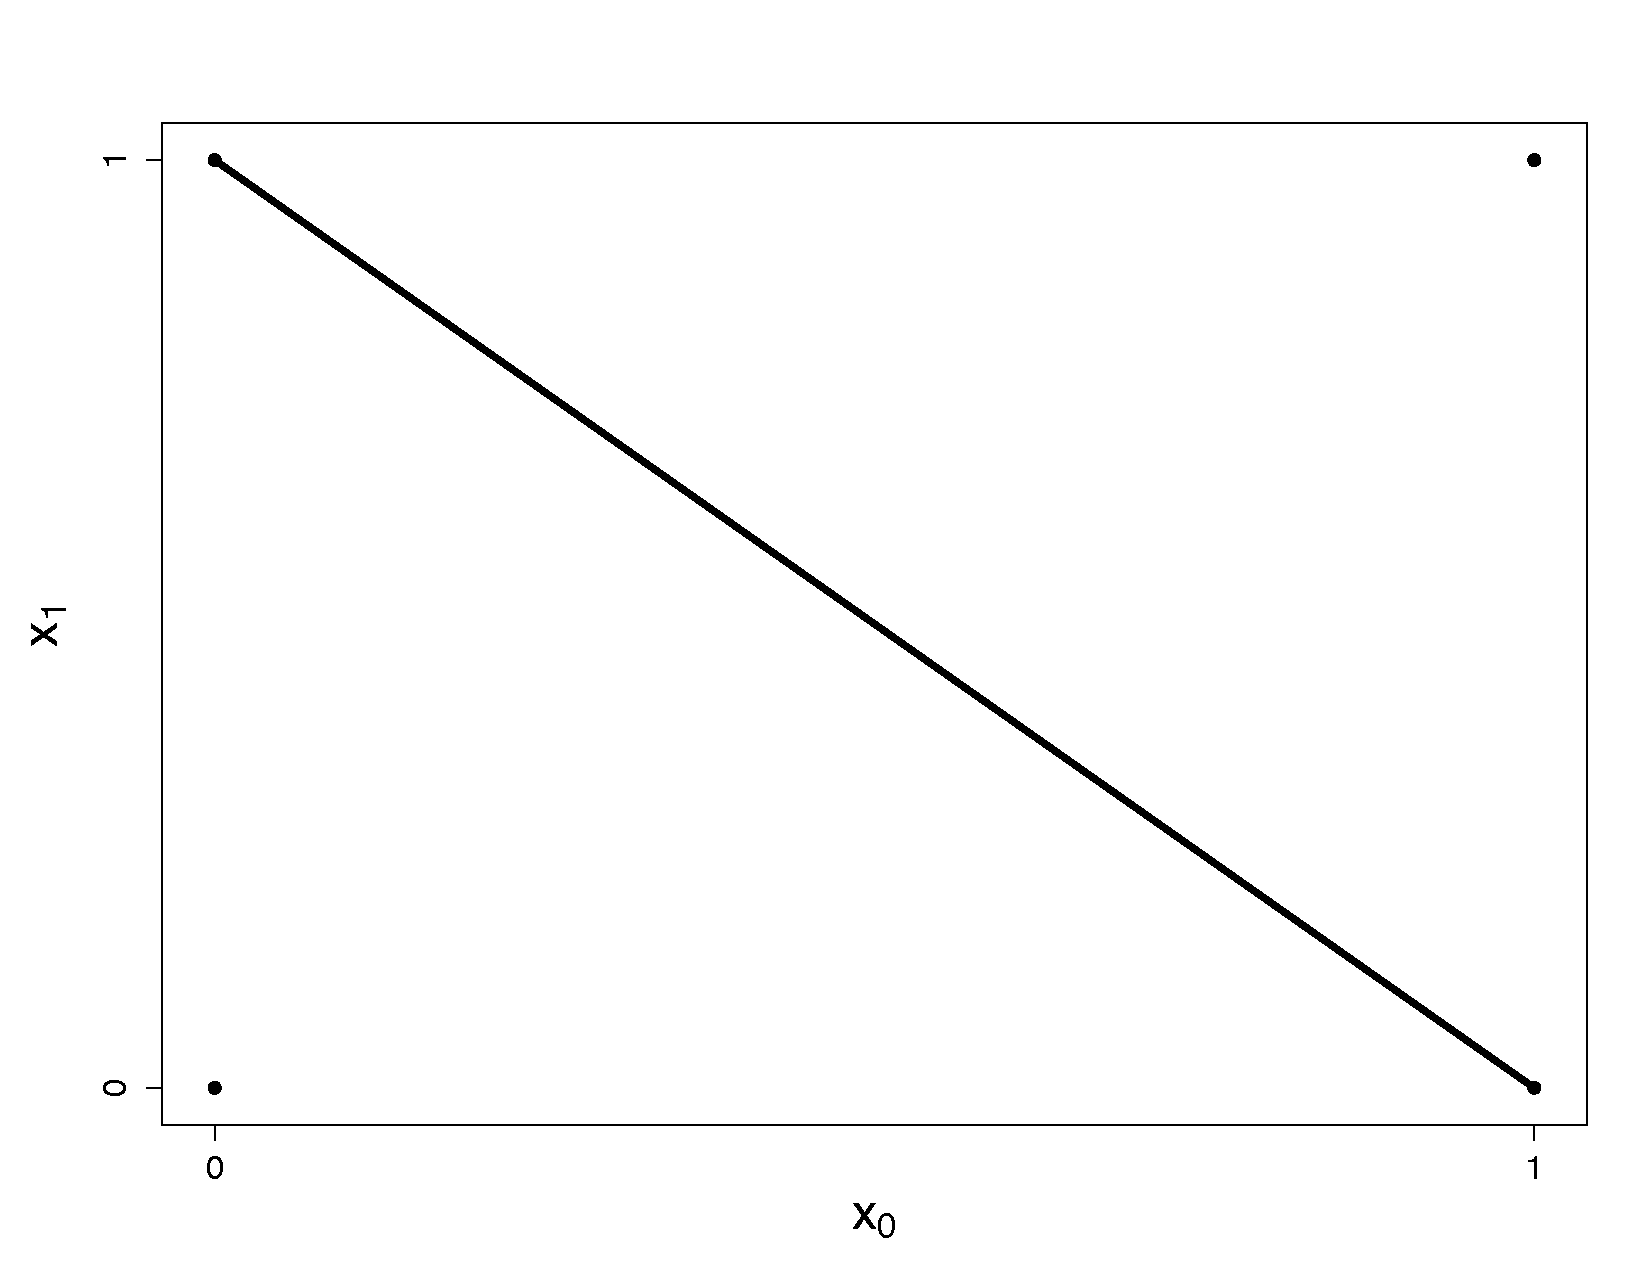
\includegraphics[width=.5\textwidth]{lewis-phase-portrait-senders}	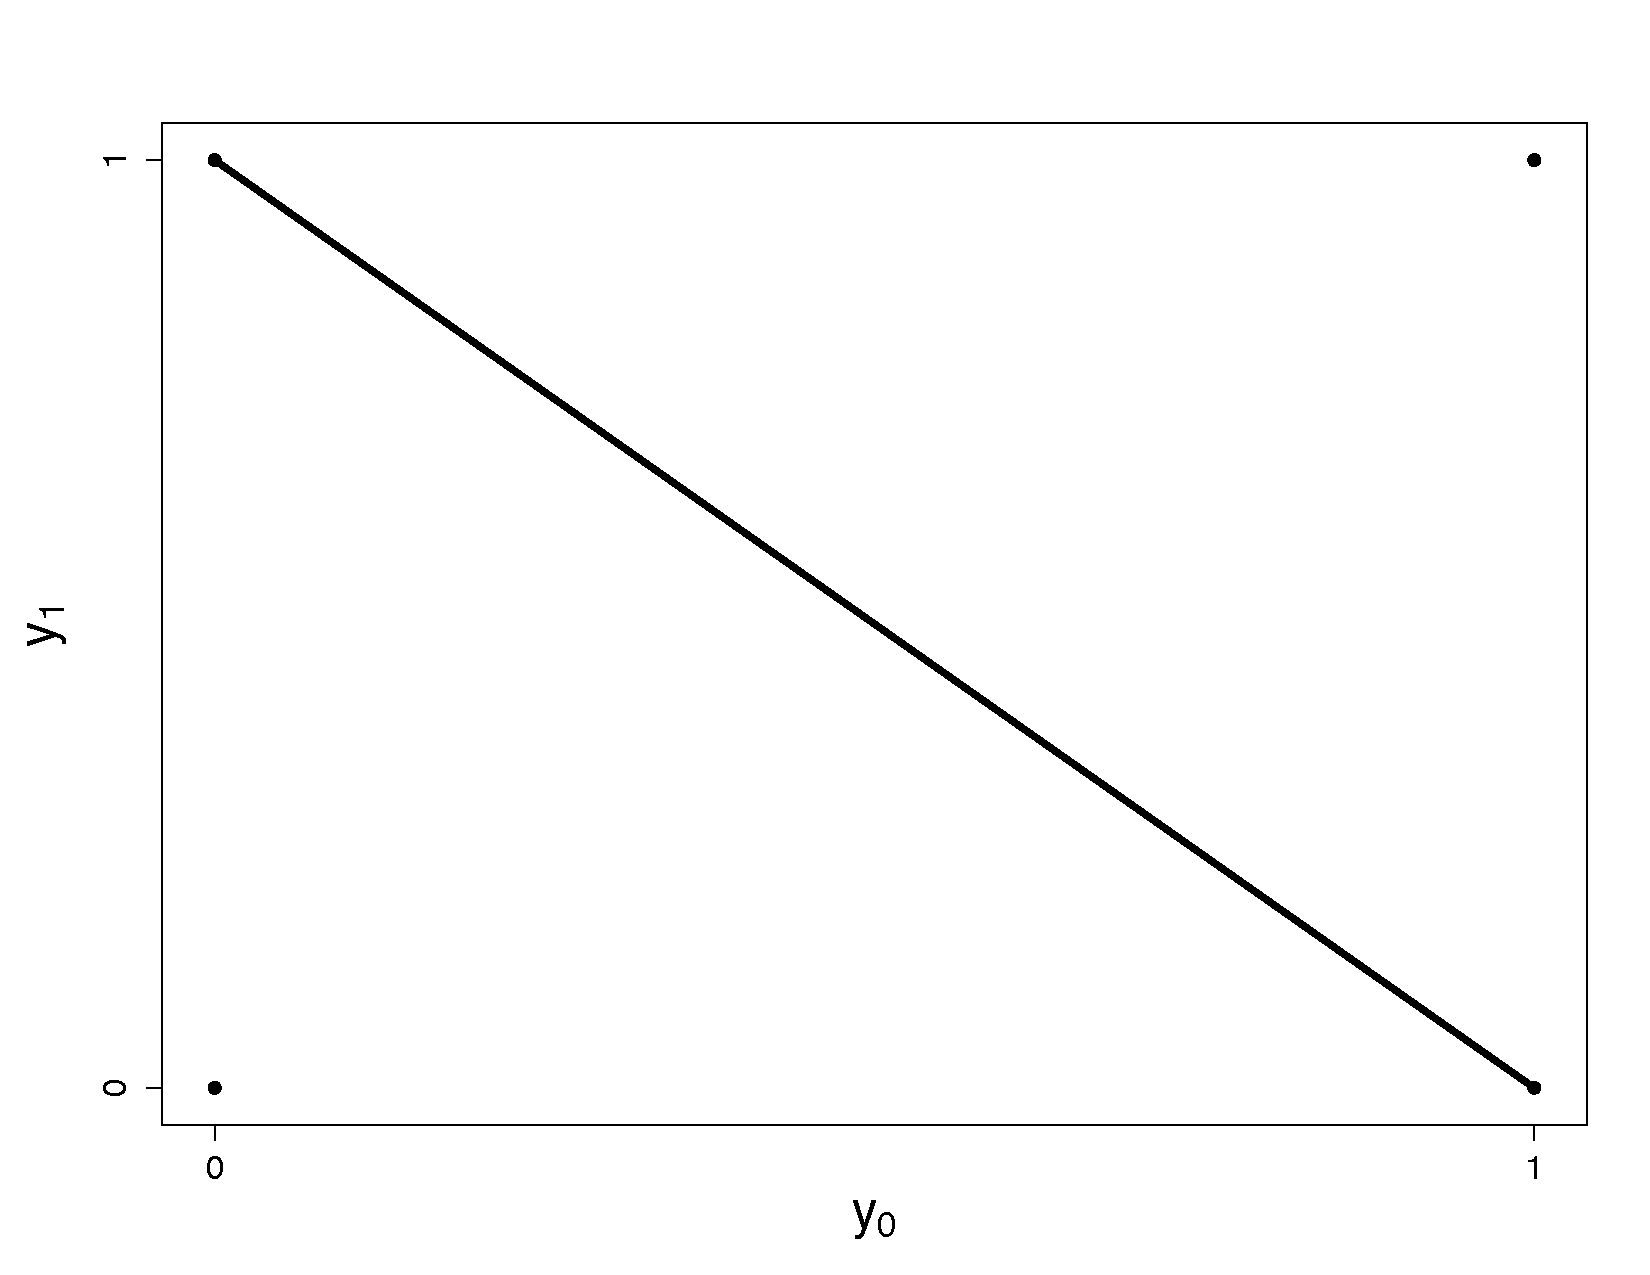
\includegraphics[width=.5\textwidth]{lewis-phase-portrait-receivers}		
%\end{figure}
%

% The structure of the signaling game along with the game dynamics specify the trajectory of the population over time through a large dimensional space. By definition, evolutionarily stable strategies constitute rest points of the replicator equations. But, in those cases where no evolutionarily stable strategies exist, the game dynamics specify the long-term behavior of the population by allowing us to characterize the stability properties of existing rest points.

% Cycles
\chapter{Cycles}
\label{cycles}

\setlength{\epigraphwidth}{.9\textwidth}
\epigraph{
[T]o say what a word means in a language is to say what
it is in general optimal for speakers of that language to
do with that word, or what use they are to make of it.\\--H.P. Grice \citeyearpar[299]{grice1989}

I can't say `It's cold here' and mean `It's warm here' -- at least, not without a little help from my friends.\\--David Lewis}


Distinguishing between the formal and functional Jespersen cycles clarifies what needs to be explained. The functional cycle can occur independently of the formal cycle, so we need an explanation for it regardless. This motivates our focus in this chapter on the functional cycle. That is, we want to know why one form displaces another, taking over the meaning of plain negation. We also want to know why this new form can be displaced in further functional cycles. In particular, we want to explain why in the history of  English we observe emphatic \emph{\textcolor{blue}{ne...not}} increase in frequency and displace pre-verbal \emph{\textcolor{red}{ne}}. To do so, we build a mathematical model of the pragmatic pressures that lead to this transition. 

First, we provide an interpretation of the notion that the incoming form is \emph{emphatic} with respect to the incumbent form,  that it conveys some special meaning. Namely, we note that the incoming form is initially restricted to contexts where the proposition being negated has just been introduced into the discourse, but expands to contexts where it is merely inferable from the discourse, and eventually to contexts where the proposition is brand new to the discourse. Second, we discuss experimental evidence that suggests why the incoming form spreads across contexts in the way it does. Speakers have difficulty in separating out their own private knowledge from what is common knowledge between themselves and their interlocutors. Given this difficulty, speakers adopt a heuristic that biases them towards their own perspective when assessing how closely connected a negated proposition is to the discourse. This leads  speakers to treat propositions as more connected to the discourse than is warranted. Third, we incorporate these facts into a signaling game, determine the equilibria and dynamics, and show how the number of signals used interacts with speaker bias. Finally, we fit the resulting model to data from the functional cycle in Middle English and discuss the implications of the fitted parameters in light of the experimental evidence. 

%Finally, we  compare the proposed model of the functional cycle to other potential explanations.

%,  In particular, the incoming form is initially restricted to contexts where the proposition being negated has just been introduced into the discourse, and is present to the attention of the interlocutors. But, as the incoming form increases in frequency it spreads to contexts where the proposition being negated is less closely tied to the preceding discourse. The goal of this chapter is to explain the dynamics of this change, and thus the functional cycle.


The main contributions of this chapter are twofold. The first contribution is that we offer the first explicitly dynamic model of the functional cycle that explains why the discourse constraints change in the manner that they do. While previous accounts have noted the constraints on the different forms of negation in the functional cycle, they have not explained the increase in the incoming form beyond the somewhat circular claim that the incoming form is overused. Here we argue that the functional cycle is a byproduct of our cognitive limitations in tracking common knowledge. Importantly, while the the driving force of the cycle is rooted in the cognition of individuals, it leads to change because of the social interactions between individuals in a population. In Grice's terms, the optimal use of and response to different forms of negation are both moving targets. Their coupled movement is what underlies the functional cycle. 

The second contribution of this chapter is that the model we present offers an information-theoretic foundation for grammaticalization. For example, the intuitive notion of \emph{bleaching} is simply the loss of information carried by a signal as it becomes obligatory. Grounding qualitative terms in this quantitative framework offers a new perspective on diachronic changes in how meaning is signaled. Moreover, it allows for a broader conception of meaning as the information carried by linguistic signals. This broader conception of meaning has the potential to unify our analyses of semantic, pragmatic, and sociolinguistic meaning.

%The meaning of any linguistic expression is a function of its use in context. In particular, speakers and hearers use grammar to signal meaning and this use is based on principles of bounded rationality. Use is publicly available and regulated by conven- tions. Although mental representations play a causal role in use, meaning is ultimately socially regulated. Clark 284





\section{Emphasis as activation}

We begin with the intuitive notion of \emph{emphasis}. We know it when we hear it, but what it amounts to is often left implicit in accounts of the functional cycle. There are two general functions that have been suggested as candidate interpretations. The first is that emphatic negation widens and strengthens negation to preclude exceptions  \citep{kadmon-landman1993any}.  That is, emphatic negation signals a stricter \emph{standard of precision} for interpreting a proposition (cf. \citealt{austin1962,lewis1970,landman1991,krifka1995polarity}). The second interpretation is that emphatic negation serves to deny an expectation, or mark the contradiction of a potentially implicit assertions \citep{detges-waltereit2002, kiparsky-condoravdi:2006}. That is, emphatic negation signals the relationship between the proposition being negated and the preceding discourse. In what follows we focus exclusively on this second interpretation, but return to the first later on as an important point of comparison.

%We return to the first interpretation later on in our discussion, but focus on the second in what follows.

Broadly speaking, this second interpretation of emphasis depends on the joint attention of speakers and hearers (cf. \citealt{chafe1974,prince1981}). More precisely, emphatic negation has been found to signal that the proposition being negated is \emph{activated} \citep{dryer1996,schwenter2005,schwenter2006}.  A proposition is \emph{directly activated} if its contents have just been explicitly introduced into the discourse, so it is present to the joint attention of speakers and hearers. A proposition is \emph{indirectly activated} if its contents can be inferred from the discourse either via an entailment or implicature.  A proposition is \emph{non-activated} if its contents have not been explicitly introduced into the discourse or it cannot be inferred from the preceding discourse.

There are two important things to note about activation. First, activation does not entail belief, nor vice versa. Participants in a discourse believe propositions that are not activated, and not all of the activated propositions are believed. This distinguishes activation from the notion of \emph{common ground} \citep{stalnaker1978}, which consists of the set of propositions that both interlocutors believe to be true, or at least accept as true for some purpose \citep[715-720]{stalnaker2002}. Second, and related to this first point, emphatic negation can be used both to negate an activated proposition or restate it. For example, if the activated proposition is $p$ then negation can be used to negate that $p$. If the activated proposition is $\neg p$ then negation can also be used to restate that $\neg p$.

Crucial for our purposes is the fact that activation can reasonably be identified in historical corpora with the use of modern translations. Moreover, activation has been shown to have the same effect diachronically in the histories of French \citep{hansen2009,grieve-smith2009}, Italian \citep{hansen-visconti2009, hansen-visconti2012}, and English \citep{wallage2013}: the incoming emphatic form in all of these languages is initially restricted to use with either activated or directly activated propositions.  For example, \cite{wallage2013} shows that in Early Middle English  \emph{\textcolor{blue}{ne...not}} is overwhelmingly restricted to negating activated propositions. But, over time it spreads to negating non-activated propositions as well. 

The following examples from the \emph{Penn Parsed Corpus of Middle English} \citep{ppcme2} cited by \cite{wallage2013} demonstrate the transition. First, the emphatic form is restricted to contexts where it is used to negate directly activated propositions. Where $p =$``They are deceived", emphatic negation can be used to deny the explicitly stated proposition that $p$. In all of the examples that follow, $p$ and $\neg p$, or both are bolded in the translation of the passage.

% Old and Middle English characters
%http://tex.stackexchange.com/questions/111032/middle-english-yogh-character


\exg. Alle \textipa{D}o men \textipa{D}e swinke\textipa{D} on \textipa{D}essere swinkfulle world, alle he swinke\textipa{D} for sumere hope \textipa{D}e hie habbe\textipa{D}, \textipa{D}e hem oft eaten ande beswink\textipa{D} ... Ac \textipa{D}o \textipa{D}e swinke\textipa{D} for \textipa{D}essere eadi hope, hie \emph{\textcolor{blue}{ne}} bie\textipa{D} \emph{\textcolor{blue}{naht}} becaht \\
All the men that labour in this toilsome world, all they labour for some hope that they have, that them often at end deceives ... But those that labour for this blessed hope, they \textsc{neg} are not deceived.\\
"All the men who labor in this toilsome whorld, they all labor for some hope they have which often \textbf{deceives them} in the end...But those who labor for this blessed hope, \textbf{they are not deceived}."\\ (CMVICES,33.385, 1200 CE)

The incoming form can also be used to restate a proposition that has already been explicitly negated. For example, where $\neg p=$``You don't know yourself", it can be restated.

\exg. If u ne cnawest e seolf ... If u \emph{\textcolor{blue}{ne}} cnawest \emph{\textcolor{blue}{naut}} e seolf\\
If you not know the self ... If you \textsc{neg} know not the self\\
"If \textbf{you do not know yourself}...If \textbf{you do not know yourself}"\\ (CMANCRIW, II.80.941-948, 1230 CE)\\

Subsequently, the use of the incoming form is extended to being used to negate propositions that are only indirectly activated. For example, we might suppose that a virtuous religious rite with all the sin-cleansing properties of baptism would have some post-mortem benefits. If we take the proposition resulting from this inference to be $p = $``[That rite] opened to them the bliss of heaven", then the incoming form can be used to negate the proposition resulting from the inference.

\exg. and te lage hadde to alle te mihtes te haue\textipa{D} nu fulluht for \textipa{D}at clensede te man of sinne: swa do\textipa{D} nu fulluht ac it \emph{\textcolor{blue}{ne}} openede hem \emph{\textcolor{blue}{noht}} te blisse of heuene alse fulcneng do\textipa{D} us.\\
and the law had then all the virtues that has now baptism for that cleansed the man of sin: as does now baptism but it neg opened them not the bliss of heaven as baptism does us.\\
"And \textbf{that rite had then all the virtues which baptism now has}, for that cleansed man of sin even as baptism now does, but \textbf{it opened not to them the bliss of heaven} as baptism does to us."\\ (CMTRINIT, 87.1165, 1225 CE)\\

Similarly, the incoming form can also be used to state a negative inference. If we suppose that renouncing one's sins requires being done committing them, $\neg p = $``I cannot renounce my sins", then the incoming form can be used to state the proposition resulting from this negative inference.

\exg. Ich nam noht giet sad of mine sines and forti \emph{\textcolor{blue}{ne}} mai ich hie \emph{\textcolor{blue}{noht}} forlete.\\
I not-am not yet sated of my sins and therefore neg can I them not renounce\\
``\textbf{I am not yet sated of my sins} and therefore \textbf{I cannot renounce them}."\\ (CMTRINIT, 75.1028, 1225 CE)

Finally, the incoming form can be used to negate propositions that are entirely new to the discourse. That is, \emph{\textcolor{blue}{ne...not}} is used to negate a proposition that is not readily identifiable either directly or indirectly from what has come before. It is useful to note that all of these examples come from roughly contemporaneous documents. 

%\footnote{Here the ordering of the elements of the bipartite form is due to negation being in an embedded clause without verb movement.}

%\exg. And here wune\textipa{D} on wanrede and tole\textipa{D}his unwilled,
%	hwile druie and hwile wete hwile chele
%	wile hete hwile hunger wile
%	turst...hwile unhele hwile sorinesse and wile
%	 werinesse and hwile wurmene cheu and fele o\textipa{D}re
%	 te ich telle ne mai and ne mai wi\textipa{D}uten helpe
%	  him seluen terwi\textipa{D} werien.\\
%	  and here dwells in distress and suesrs his discomfort,
%	  sometimes dry and sometimes wet sometimes cold
%	  sometimes hot sometimes hunger sometimes
%	  thirst...sometimes sickness sometimes soreness and sometimes
%	  weariness and sometimes worm�s biting and many others
%	  that I tell neg can and may without help
%	  himself therewith protect\\
%	  "and here he dwells in distress and endures discomfort, sometimes dry and sometimes wet, sometimes cold and sometimes hot, sometimes hunger, sometimes thirst, sometimes sickness sometimes soreness, sometimes weariness and sometimes the biting of worms, and many others that I cannot tell of, and may not protect himself against them without help"\\ (CMTRINIT, 123.1648)


%\exg. Hit was on mann, dedlich alswa we bie\textipa{D},
%	and he besohte at gode tat naht ne scolde reinin, for
%	\textipa{D}e folc to kastin. Godd him ihierde � tat was Helyas
%	� and wi\textipa{D}held alle reines trie hier and six monetes...�\\
%	It was a man mortal as we are,
%	and he besought of God that \emph{\textcolor{blue}{not}} \emph{\textcolor{blue}{ne}} should rain for
%	the people to chasten. God him heard � that was Elias
%	� and withheld all rains three years and six months...\\
%	``There was a man, mortal as we are, and he besought God that \textbf{it should not rain}, to chasten the people. God heard him � that was Elias � and withheld all the rains three years and six months...''\\
%	(CMVICES1,143,1787)\\
	
%The condition factors of the incoming form can be stated in the following manner. Initially, the incoming form is sensitive to the activation of the proposition it negates, but ceases to be over time. As the incoming form increases in frequency it stops being used exclusively to negate activated propositions, eventually being used to negate both activated and non-activated propositions. 



% Once the incoming form is used to negate propositions for any degrees of activation it ceases to carry any specialized meaning.
%As we noted above, for English, \emph{\textcolor{blue}{ne...not}} overwhelmingly occurs in contexts where it is negating an activated proposition. Subsequently, the embracing form increases in frequency and is used in more and more contexts with a wider range of degrees of activation. As it is used in more and more contexts it loses its specialized meaning. At the end point of the functional cycle, where the embracing form is used across all contexts, it ceases to carry any specialized meaning. Thus, the functional cycle can be conceived of as of one form taking the place of another along a continuous semantic dimension.

%The first bias that speakers have is that they tend to overestimate how easy it is to infer communicative intentions.  \cite{savitsky-etal:2011} had two pairs of friends participate in a simple communication task. All four participants sat back to back and were individually given lists of four-way ambiguous sentences to read out loud with a specified meaning. For example, the sentence ``It's getting hot in here.'' could be interpreted as an indirect request to open the window or an amorous advance. Participants were asked to do two things. They were asked to guess the intended meaning of the sentences spoken by the other participants from the list of four potential meanings. They were also asked to estimate how many of the sentences the friend they came with had guessed correctly, and how many sentences the strangers from the other pair had guessed correctly. 
%
%Hearers were reliably above chance at guessing the intended meaning out of the four potential meanings, but, friends and strangers did not differ significantly. However, speakers had much higher expectations for hearers. Speakers significantly overestimated how many sentences hearers would accurately guess. This suggests that, as speakers, we often tend to overestimate how transparent our utterances actually are to our hearers, expecting them to readily read our minds and infer the privileged information therein.
%

\section{Experimental evidence regarding activation}


While we observe this trend in historical corpora of English and other languages, this does not explain why the incoming form spreads across the contexts in the way it does. To understand why, it is useful to consider  experimental evidence demonstrating particular communicative biases on the part of speakers. Namely, speakers' private knowledge persistently influences how they signal meaning.

For example, \cite{wu-keysar2007} had pairs of participants play a communication game in fixed roles of speaker and hearer. Speakers and hearers jointly learned names for a set of abstract shapes. Speakers then learned several names for additional shapes privately. The experimenters varied the number of shape names that the speaker and hearer learned together, what the experimenters called the \emph{informational overlap} between participants. The participants then played a game where the speaker directed the hearer to select a target shape from a set. Across trials the target shapes were evenly distributed between shapes whose names were learned together, shapes whose names were learned privately by the speaker, and shapes that were new to both participants. Presumably, using a name to refer to a shape is only felicitous if the name of the shape was learned together by both speaker and hearer. But, surprisingly, in trials where the target shape's name was private knowledge, the name was the first thing speakers said in 5\% of trials where there was a low informational overlap and in 28\% of trials where there was a high informational overlap. That is, speakers relied on their private knowledge more where there was a greater degree of informational overlap.

Note that this use of the privately known names was not a result of speakers forgetting the context in which the names were learned. \cite{heller-etal2012} replicated these findings and showed that speakers were incredibly accurate at distinguishing between names learned together versus names learned privately. Rather, \citet[4]{wu-keysar2007} suggest that these results point to speakers using a kind of \emph{overlap heuristic}: when the informational overlap between yourself and your interlocutor is sufficiently extensive act \emph{as if} they have all the same information as you. In fact, this is kind of combined \emph{co-presence} and \emph{community membership heuristics} proposed by  \cite{clark-marshall1981} to resolve the problem of \emph{common knowledge}: that everyone knows that $p$, that everyone knows that everyone knows that $p$, \emph{ad infinitum}.\footnote{This technical term was introduced into the Philosophical literature by \cite{lewis:1969}, but has a long history under various names. Whereas \cite{clark-marshall1981} use the term ``mutual knowledge'' to refer to common knowledge, as it is commonly used \emph{mutual knowledge} only requires that everyone know that $p$. Thus anything that is common knowledge is also mutual knowledge, but not \emph{vice versa}.}  This heuristic and the speaker bias that it creates are a means for solving the difficult task of keeping track of what is private versus common knowledge.  Assuming that an interlocutor knows roughly the same things about the world  reduces the cognitive burden and simplifies things a great deal.

%That is, speakers could not undo this bias if they simply  tried harder to keep track of what was common versus private knowledge.

However, given that speakers' use of private knowledge varied across conditions, we might wonder whether this bias is specific to certain contexts. For example, speakers might be able to pay closer attention to the discourse and keep better track of things. That is, there might be two modes of thinking regarding the discourse \citep{keysar-etal2003, kahneman2011}. However, this bias is not subject to conscious manipulation.  \cite{lane-etal2006} had pairs of participants play a communication game in fixed roles of speaker and hearer. Four shapes of varying size and color were presented to the participants. One shape was visible to only the speaker, blocked from the view of the hearer by an occluder. Speakers were instructed to communicate information about a target shape visible to both participants so the hearer could identify it. In the test conditions, the item that was visible only to the speaker was the same shape as the target item, but varied along some relevant dimension (e.g. size, color).  For example if the target shape was a blue triangle then the shape that was only visible to the speaker was a green triangle, and none of the other shapes visible to both participants were triangles.

\cite{lane-etal2006} found that speakers modified their description more in the target condition. That is, speakers were more likely to say ``The blue triangle" to refer to the target shape if there was a green triangle visible only to them. Speakers' private information leaked into what they said and how they said it. This happened even though speakers had direct evidence that only they could see the shape that contrasted with the target shape. In fact, this over-modification happened to an even greater extent when speakers were explicitly instructed to conceal information about their privileged information. Speakers have a difficult time inhibiting their perspective even when they want to, suggesting that speaker bias is persistent fact about communication.

These experimental results show how speakers' private knowledge persistently influences how they signal meaning. In particular, they show that speakers tend to assume that their interlocutors are overwhelmingly similar to them. While this experimental evidence deals with the referential domain, the results can be extrapolated to the propositional domain and activation in particular. That is, activation is defined by the joint attention of speakers and hearers. But, neither speakers nor hearers know whether or not a proposition is actually being attended to by an interlocutor.  This problem is a perfect candidate for solution by the kind of heuristic described above. Namely, speakers can simplify the problem by assuming that what their hearers attend to is sufficiently similar to what they attend to.

One potential concern about this kind of heuristic is that mistakes seem unlikely. If a proposition is directly activated, then it is directly activated because it has just been mentioned. Similarly, if a proposition is indirectly activated, then it is indirectly activated because there is an entailment or implicature that does so. A response to these objections, particularly the first, lies in the nature of activation. While we have described discrete categories, \citet[481-482]{dryer1996} rightly conceives of both direct and indirect activation as continuous measures.  For example, while the utterance of a proposition directly activates it, this activation decays over time. As he puts it, the proposition is \emph{deactivated} as time goes on and it passes from the joint attention of speakers and hearers.  Similarly, while the utterance of one proposition may indirectly activate another via an inference, some propositions may be more \emph{accessible} than others via inference.  Some inferences are natural, whereas others are non-sequiturs. In fact, we might take activation as a whole to be constituted by degrees of inferability. Recently uttered propositions are high on the scale, whereas brand new propositions are at the bottom end.

%As a whole then, we can think of activation as a continuous scale. Propositions that have just been uttered have the highest degree of activation, and are at the top of the scale. Propositions that have no connection to the discourse have the lowest degree of activation, and are at the bottom of the scale. The functional cycle consists of the spread of the incoming form from being associated with high degrees of activation to lower degrees.

So, speakers might treat a proposition as more activated than is warranted for several reasons. For example, suppose that a speaker keeps thinking about a proposition $p$, but her interlocutor does not. This means that $p$ is being deactivated as it has passed from the joint attention of both participants. However, the speaker still dwelling on $p$ is not aware of this, and only has her own perspective to consider.  Thus, she may still treat $p$ as highly activated even though it is not. Similarly, a speaker may easily infer a proposition $p$ from the preceding discourse due to her attention to particular aspects of the discourse. But, her interlocutor may only make the same inference with great effort. Thus, a speaker may treat $p$ as highly activated even though it is not. 

%In both cases, speakers cannot peer into their interlocutor's head, so they take their own head as a reasonably good model. This heuristic biases speakers towards their own private knowledge, and has implications for how forms that are sensitive to private versus common knowledge are used over time. This is certainly true for activation since it depends on this distinction between private and common knowledge. 

If speakers have a tendency to overestimate activation and use \emph{\textcolor{blue}{ne...not}} more than is warranted by the actual degree of activation, then how will hearers respond? Given hearers' response, how will speakers respond in turn? What does this mean for the functional cycle? To answer these questions we translate these experimental findings into a mathematical model that can be used to investigate meaning over time. This model consists of two components. First, we define the \emph{stage game} that describes the interactions between speakers and hearers and captures speakers' bias towards overestimating activation. Second, we define the \emph{game dynamics} that describe how a population of speakers and hearers change over time while playing the stage game. 

%We begin by defining the stage game and determining the evolutionarily stable strategies of the game, and then turn to the dynamics of a population.

\section{A signaling game model of emphasis}

We start by defining the components of the stage game that we will use to analyze the functional cycle. We define the states, messages, and actions along with their interpretations. We then turn to the utility function of senders and receivers as they relate to the preferences of speakers and hearers. Once we define the game we can determine its equilibria and the dynamics of how speakers use different forms of negation to signal the activation of the proposition being negated.

%meaning is signaled over time.

First, let the set of states $T : [0,1]$ be the degree of activation of the proposition being negated, where $t = 0$ indicates a brand new proposition and $t = 1$ indicates a proposition that was the last thing uttered.  Second, let the set of messages that the speaker sends be a finite set $M = \{\textcolor{red}{m_1},  \textcolor{blue}{m_2}\}$. We can think of these as the incumbent and incoming form in the functional cycle respectively. So, for English, $\textcolor{red}{m_1}$ is \emph{\textcolor{red}{ne}} and $\textcolor{blue}{m_2}$ is \emph{\textcolor{blue}{ne...not}}. Finally, let the set of actions $A : [0,1]$ be the action taken by the hearer to interpret the message. For example, an action $a_i$ can be thought of as an initial guess by the hearer about the level of activation $t_i$ of the negated proposition. 

%the hearer reasoning about whether a proposition with levels of activation successively further from $t_i$ would be incorporated into the discourse.

%In what follows we will interchangeably refer to speakers as senders and hearers as receivers.

%This means that we expect $\textcolor{blue}{m_2}$ to increase over time as part of the functional cycle. 

With these components defined, it is important to make a conceptual clarification about the role of states as degrees of activation. In signaling games, the state is taken to be some piece of private information that the sender has about the state of the world. This is not quite accurate given that we assume that speakers never know the actual degree of activation. That is, they can never peer inside hearers' heads to verify what propositions are being attended to at any given moment. At best, speakers have a subjective estimate of the degree of activation. However, this subjective estimate is systematically related to the actual degree of activation.

To see this, suppose that both speakers and hearers have some subjective estimate of the activation of a proposition, call them $t_S$ and $t_R$. For example, both might take their estimate to be the approximate amount of attention they are paying to a given proposition.  Now, given that activation is defined in terms of the joint attention of speakers and hearers, then the actual state of activation $t$ must be some function of the two subjective estimates. If a speaker's estimate of a proposition is that it is not activated $t_S = 0$ because she is not attending to it, then by definition it is not activated $t = 0$.  In contrast, if a speaker's estimate of a proposition is that it is highly activated $t_S=1$, this does not mean that it is indeed activated since the hearer's estimate could be lower $t_R < 1$ because the hearer is not attending to it to the same degree. 

%Note that both of these follow from the definition of activation in terms of the joint attention of speakers and hearers

A simple way of capturing the relation between the subjective estimates and the actual degree of activation is that $t = min(t_S, t_R)$. The actual level of activation is the highest degree that both participants would agree to based on their own subjective estimates. This is arguably what underpins our intuition that a form is infelicitous because a hearer did not or could not have had a sufficiently high subjective estimate of activation. If this is the relation between the subjective estimates and the actual state, the speaker's estimate stands in a particular relation to the actual state. Namely, the speaker overestimates the degree of activation. To see why, note that if $t_S \leq t_R$ then $t_S = t$, and if $t_S > t_R$ then $t_S > t$. Together these imply that $t_S \geq t$. In other words, on average the speaker overestimates the actual degree of activation.

Now, if speakers only have access to their own subjective estimates of the state of activation, then it makes sense that their preference are determined by that estimate. As far as the speaker is concerned, $t_S$ is the actual degree of activation of the proposition being negated. It makes sense then that the speaker would want the hearer to infer that degree of activation. In particular, we suppose that speakers prefer for hearers to infer the degree of activation that is closest to their subjective estimate. The following utility function satisfies this constraint, it is maximized exactly where $a = t_S$.

\begin{equation}
     U_S(t, a) = 1 - (a - t_S)^2
\end{equation}
While this function captures the speaker's preferences, it also introduces a new and undefined parameter, the speaker's subjective estimate. A simple way to address this is  to posit a general functional shape $f(t) = t_S$  that is defined in terms of the actual state and other parameters but captures speakers' tendency to overestimate the actual state by guaranteeing that $f(t) > t$.  There are infinitely many functions that satisfy this constraint, but a particular simple functional form has a natural interpretation in our case. 

In their seminal work on signaling games of \emph{information transmission}, \cite{crawford-sobel:1982} introduce a bias parameter $b \geq 0$ into the utility function of senders that indicates how aligned the goals of senders and receivers are. For example, where $b=0$ their preferences are perfectly aligned, but for $b > 0$ they diverge. We can apply this directly to our case if we think about the bias parameter $b$ as speakers' tendency to overestimate activation. Then the following simple linear function allows us to incorporate the tendency to overestimate into the speaker's utility function.

\begin{equation}
	t_S = f(t) = t + (1-t)b
\end{equation}
This yields the following utility function which satisfies the constraint that $t_S \geq t$.\footnote{This differs from the formulation in \cite{crawford-sobel:1982} where $U_S(t,a) = -(a - t - b)^2$. Their form allows senders to prefer actions $a > 1$, which has no interpretation in our model. That is, the degree of activation and interpretation of the degree of activation are both constrained to the unit interval. We also add a constant so that all payoffs are positive for the dynamic analysis in the next section.} It is maximized for an action $a = t + (1-t)b$. This means that speakers prefer that hearers take an action slightly higher the actual state of activation.

\begin{equation}
     U_S(t, a) = 1 - (a - t - (1-t)b)^2
\end{equation}
By changing the variables we obtain a functional form that depends only on states, actions, and the new bias parameter. In fact, this bias parameter has a natural interpretation in terms of speaker bias as a measure of how good or bad speakers are at keeping track of common versus private knowledge. The case where $b=0$ corresponds to speakers developing the ability to read minds and accurately assess the actual state of activation. For $b > 0$ speakers have a tendency to overestimate the degree of activation and prefer a higher action on the part of hearers. 

Now, we might wonder whether speakers have access to the action taken by hearers. That is, if speakers cannot peer into the heads of hearers to determine the state of activation, does it makes sense to assume that they can somehow infer the reasoning process indicated by the action hearers take to interpret the message? However, speakers have incredibly rich sources of feedback from hearers. For example, this feedback includes the amount of time hearers take to respond, facial expressions, and backchannel cues (e.g. ``Mhmm'' versus ``Huh?''), as well as verbal responses such as as requests for clarification or continuations of the discourse.  All together then, it seems reasonable that speakers can recover the action taken by hearers.

% Potential note about how speakers and hearers get "feedback"
% Why/How do hearers have access to actual state of activation?

With speaker preferences defined, we can think about hearers. Suppose that hearers want to accurately infer how the proposition being negated relates to the prior discourse. For example, a hearer does not want to overestimate the degree of activation of a proposition and expend too much effort on trying to discern how it is connected to the discourse. Similarly, a hearer does not want to underestimate the degree of activation and miss out on information regarding how a proposition fits into the discourse.  The following utility function satisfies this constraint, it is maximized exactly when $a=t$.

%\footnote{A more sophisticated analysis might incorporate the receiver's subjective estimate into her interoperation of the message given the prior probability distribution.}
%That is, hearers do best when they invest the appropriate amount of effort towards integrating what the speaker says into the discourse.  

\begin{equation}
     U_R(t, a) = 1 - (a - t)^2
\end{equation}
That is, hearers do best when they accurately infer the actual degree of activation. Now, we might wonder again whether it is reasonable to assume that hearers have access to the actual degree of activation. They cannot read minds any more than speakers. However, hearers gain information as they reason about different potential degrees of activation. 

To see why this is the case, first assume that speakers and hearers have the same reasoning capacities. That is, they would agree on what potential degrees of activation make some kind of sense given the discourse. So, we assume that speakers and hearers can both identify a particular set of degrees of activation as making sense. Note that this does not require that speakers and hearers expend the same amount of effort in identifying the degree of activation, but rather that speakers and hearers have the same reasoning capacities. Here we will suppose that there is some function of states given the discourse that defines whether both speakers and hearers can identify a particular degree of activation. Namely, let $g(t)$ be a convex function such $g(t) = 1$ if and only if $t$ can be identified by both speaker and hearer. Further, suppose that the lowest identifiable degree of activation corresponds to the actual state of activation, for all $t_i < t$, $g(t_i)=0$. This simply means that the subjective estimates of speakers and hearers serves as a lower bound on what degrees of activation both speakers and hearers can reasonably identify.

Now, suppose that hearers reason in the following manner when they take an action to interpret the speaker's message. The hearer takes an action $a_i$, corresponding to an initial guess that the degree of activation of the proposition is $t_i$. By the same reasoning for speakers above, hearers overestimate the actual degree of activation $t_R \geq t$, so it makes sense that they would compensate for this by choosing an action such that $t_i < t_R$. Given this action, there are two possibilities. The degree of activation for the proposition could be identifiable or not. If the initial guess of the degree of activation is identifiable $g(t_i)=1$, suppose that the hearer reasons about lower and lower degrees of activation; likewise, if the initial guess of the degree of activation is not identifiable $g(t_i)=0$, suppose that the hearer reasons about higher and higher degrees of activation. In both cases the hearer will consider a degree of activation $t_j$ such that $g(t_j) = 1$ and for all $t_k < t_j$, $g(t_k) =0$.  That is, she will eventually recover the actual degree of activation.  Note also that the amount of effort put into finding the actual degree of activation grows with the distance between the initial guess and the actual degree. So, if speakers and hearers reason in a sufficiently similar manner, then hearers will be able to recover the actual state of activation.

The preferences we have defined for speakers and hearers are a way to represent the experimental evidence we described in the previous section. That is, they allow us to state, in mathematical terms, the stage game which is the shape of the interaction. But, this shape by itself does not make any predictions about the behavior of individual speakers and hearers playing the game or the trajectory of a population of speakers and hearers over time. To understand these we need to determine the equilibria of the stage game and how a population changes while playing the stage game under a particular game dynamics.

%To understand these we need to address the static properties of the stage game
%we need to determine the equilibria of the game and supply a game dynamics. 

%With thes components of the game defined, we now turn to analyzing the equilibria of the game. In particular, we examine how the implications of the game for the functional cycle.


\section{Equilibria of the signaling game}

Now that we have defined the components of the game, we turn to analyzing its properties. Determining the equilibria of the game we described will allow us to address several questions about how signals are used in the functional cycle. Broadly speaking, we want to know two things. First, we want to understand the relationship between senders' bias towards overestimating activation and the use of signals at equilibrium. In particular, we want to know how large this bias can be while still allowing for multiple forms to be used at equilibrium. Second, we want to know whether particular equilibria constitute evolutionarily stable strategies. If so, we want to know the strategies that are evolutionarily stable. If not, we want to know what strategies could invade the population and disturb an equilibrium. Broadly speaking, this amounts to determining the conditions for the functional cycle to occur.  We begin by defining speaker and hearer strategies, the expected utility of different strategies, and then determine the evolutionarily stable strategies of the game. 

The set of speaker strategies is all potential mappings from the unit interval to a discrete set $S : [0,1] \rightarrow M$. This is problematic given that the domain is uncountable. To simplify things we consider the following condensed representation. Let $\mathcal{P}_n(T)$ be a partition of the state space into $n$ equal length subintervals $t_0 = 0 < t_1 < ... < t_{n-1} < t_n = 1$.  For each properly defined subinterval, $(t_{i-1},t_i)$ the sender uses the message $m_i$. A speaker's strategy is then a function from this partition to messages $S : [\mathcal{P}_n(T) \rightarrow M]$.  Intuitively, this is simply a way of carving up the state space into discrete contiguous regions and using those regions to determine which signal to send. For example, consider the case of two messages $\mathcal{P}_2(T)$, where $\textcolor{red}{m_1}$ and $\textcolor{blue}{m_2}$ correspond to \textcolor{red}{\emph{ne}} and \textcolor{blue}{\emph{ne...not}} respectively. For $t \in (0, t_1)$ a sender will use  \textcolor{red}{\emph{ne}} and for $t \in (t_1, 1)$ a sender will use \textcolor{blue}{\emph{ne...not}}.

In fact, this kind of threshold strategy is extremely close to what we observe in historical data. That is, as the functional cycle proceeds, the incumbent form \emph{\textcolor{red}{ne}} is not evenly distributed across activation contexts, but largely negates non-activated propositions. The probability of using the two negative forms is overwhelmingly conditioned by the activation of the proposition being negated. For example, for Midddle English from 1150-1250 CE the conditional probabilities are the following \citep[12]{wallage2013}

\begin{equation}
	p(\emph{\textcolor{red}{ne}} \mid  \textsc{non-activated}) = .85
\end{equation}

\begin{equation}
	p(\emph{\textcolor{blue}{ne...not}} \mid  \textsc{activated}) = .84
\end{equation}
This means that specifying speaker strategies in this manner is both a useful and empirically accurate abstraction. Interestingly, this also gives some empirical credence to the push-chain scenario conception of the functional cycle; \emph{\textcolor{red}{ne}} actually appears to be pushed down the scale of activation by \textcolor{blue}{\emph{ne...not}}.

The set of hearer strategies is all potential mappings from the set of messages to the unit interval $R : M \rightarrow [0,1]$. Since the domain is finite, this is more straightforward than the set of speaker strategies. For each message $m_i$ the hearer takes an action $a_i$. So, for example, $\textcolor{red}{a_1}$ would be the hearer's response to message $\textcolor{red}{m_1}$, in this case \textcolor{red}{\emph{ne}}, and $\textcolor{blue}{a_2}$ would be the hearer's response to message $\textcolor{blue}{m_2}$, in this case \textcolor{blue}{\emph{ne...not}}.

Now that we have defined the set of speaker and hearer strategies, we can ask what strategies constitute evolutionarily stable strategies. Given that signaling games are asymmetric, this amounts to identifying the strict Nash equilibria of the game. This can be done by determining what strategies jointly maximize the expected utilities of speakers and hearers.

\begin{equation}
     E[U_S(s, r)] = \int_T \left( 1 -(r(s(t)) - t - (1-t)b)^2 \right)p(t)dt
\end{equation}

\begin{equation}
      E[U_R(s, r)] = \int_T \left( 1 -(r(s(t)) - t)^2 \right) p(t) dt
\end{equation}
These are exactly analogous to expected utility in the discrete case, where we summed over all the possible states. Again, $r(s(t))$ is the receiver's respond to the sender's message and yields an action, which determines the utility for both sender and receiver given a state.

We estimate the prior probability over states as a \emph{beta distribution} over the set of states, parameterized by two shape parameters $\alpha$ and $\beta$, and often written as $\mathcal{B}(\alpha, \beta)$. Figure \ref{beta-distribution} shows the distribution for several values of $\alpha$ and $\beta$, including the uniform distribution $\mathcal{B}(1, 1)$. These two shape parameters gives us quite a bit of flexibility in modeling different potential prior probability distributions. We use them extensively in the analysis that follows, so we note two things that should offer an intuitive conceptual foothold. First, the expected value of a beta distribution is given by $\frac{\alpha}{\alpha + \beta}$. So, for example, the expected value of the uniform distribution is $\frac{1}{2}$ given that $\alpha=\beta=1$, which is what we see in Figure \ref{beta-distribution}. Second, if we fix $\beta=1$ and let $\alpha$ vary, then the distribution will be more and more skewed to the right as $\alpha$ grows larger. This also follows from the fact that the expected value $\frac{\alpha}{\alpha  + 1}$ gets closer and closer to one as $\alpha$ grows. Note that the mirror image case would hold if we fixed $\alpha=1$ and let $\beta$ vary.

\begin{figure}
\centering
     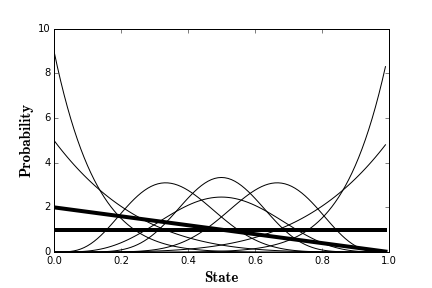
\includegraphics[width=.75\textwidth]{beta-distribution.png}
\caption{Beta distribution for various parameter values of $\alpha$ and $\beta$, including the uniform distribution $\mathcal{B}(1,1)$, and the empirical distribution $\mathcal{B}(1,2)$.}
\label{beta-distribution}
\end{figure}


We use the historical data  in Table \ref{activation-table} from \citet[12]{wallage2013} that shows the number of propositions by activation  to estimate the estimate the prior distribution over states. The degree of activation in these examples is estimated using translations of the texts. However, there are reasons to be confident that activation can reliably be identified in historical corpora.  These figures agree with similar estimates from contemporary corpora. For example, in a sample from a corpus of British English, \cite{tottie:1991} finds that negation is only used 14\% of the time with directly activated propositions. Likewise, in a corpus of American English, \cite{thompson1998} finds that negation is only used 5\% of the time with directly activated propositions. These results suggest that the prior distribution is stable, with the preponderance of negation being used with brand new non-activated propositions. Intuitively, this distribution makes perfect sense: the majority of conversation is about introducing new information rather than treading the same old ground of what has already been said. If the prior distribution is indeed stable, then we can estimate it from the data pooled across time periods. A good fit to the data is the prior probability distribution $\mathcal{B}(1,2)$, also shown in Figure \ref{beta-distribution}.\footnote{We treat each of the discrete categories as equal portions of the unit interval and find values of $\alpha$ and $\beta$ such that $\int_0^\frac{1}{3} \mathcal{B}(\alpha, \beta)(t) dt \approx p(\textsc{non-activated})$, $\int_\frac{1}{3}^\frac{2}{3} \mathcal{B}(\alpha, \beta)(t) dt \approx p(\textsc{indirectly activated})$, and $\int_\frac{2}{3}^1 \mathcal{B}(\alpha, \beta)(t) dt \approx p(\textsc{directly activated})$, where the probabilities are estimated from the totals in Table \ref{activation-table}. Obtaining a better empirical estimate of the prior from contemporary data and intuitions is something we leave for future research.}




\begin{table}
\begin{tabular}{@{}cccc@{}}
\hline
    \textsc{period}   &\textsc{non-activated} & \textsc{indirectly activated} & \textsc{directly activated} \\
\hline
1150-1250    & 393  & 203 & 52   \\
1250-1350    & 346  & 296 & 42 \\
1350-1420    & 294  & 179 & 60 \\ \hline
\textsc{total} &1033 & 678 & 154  \\
\end{tabular}
\caption{Distribution of sentence activation in PPCME \citep{ppcme2} from \cite{wallage2013}}
\label{activation-table}
\end{table}
%We have two functions that we want to maximize with respect to three variables. To do so, we need to find the conditions where the following hold.
%
%\begin{equation}
%	\frac{\partial E[U_S(s, r)]}{\partial t_1^*} = 0
%\end{equation}
%
%\begin{equation}
%	\frac{\partial E[U_R(s, r)]}{\partial a_1^*} = \frac{\partial E[U_R(s, r)]}{\partial a_2^*} = 0
%\end{equation}

To calculate the maxima of the expected utility functions, let $\langle s^*, r^* \rangle$ be an equilibrium strategy profile. In this case, the speaker strategy is defined by $s^*((0, t_1^*)) = \textcolor{red}{m_1}$ and $s^*((t_1^*, 1)) = \textcolor{blue}{m_2}$. Likewise, the hearer strategy is defined by $r^*(\textcolor{red}{m_1}) = \textcolor{red}{a_1^*}$ and $r^*(\textcolor{blue}{m_2}) = \textcolor{blue}{a_2^*}$.  We can determine the evolutionarily stable strategies by jointly maximizing speaker and hearer expected utility. That is, we solve a system of partial differential equations for $t_1^*$, $\textcolor{red}{a_1^*}$ and $\textcolor{blue}{a_2^*}$. For any amount of bias, the maximizing values are shown in Figure \ref{sol2-beta}.\footnote{See Appendix A for the full calculations of the solution.} Along the horizontal axis is the amount of speaker bias, the vertical axis represents the point at which speakers partition the state space and the actions of hearers in response to the forms. For any value of the speaker bias $b$, the solid black line represents the point at which speakers partition the state space $t_1^*$ and the dashed lines represent hearer responses to the different messages, $\textcolor{red}{a_1^*}$ and $\textcolor{blue}{a_2^*}$.

\begin{figure}
	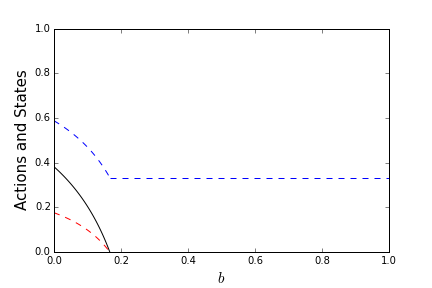
\includegraphics[width=.75\textwidth]{sol2-beta.png}
	%
	\caption{Equilibrium solution for two messages for values of bias}
	\label{sol2-beta}
\end{figure}

%So, for example, where $b=.1$ speakers will partition the states at $t_1^*=$, sending $\textcolor{blue}{m_2}$ for all states above this point and sending $\textcolor{red}{m_1}$ for all states above. In response to these forms, hearers will take the actions indicate by the dashed lines, $\textcolor{red}{a_1^*} = $ and $\textcolor{blue}{a_2^*} = $. In fact, these actions correspond to the expected value of the state given the message. That is, $\textcolor{red}{a_1^*} = E[t \mid t < t_1^*]$ and $\textcolor{blue}{a_2^*} = E[t \mid t > t_1^*]$. They are the \emph{Bayes estimators} of their respective signals, the values that maximize hearers' expected utility given a signal.


We are now in a position to answer our first question regarding the relationship between speaker bias and the use of different forms at equilibrium. Namely, if speakers are too biased when it comes to keeping track of common versus private knowledge then only a single message can be used in equilibrium. For example, we can read off of Figure \ref{sol2-beta} that if $b > \frac{1}{6}$ then only $\textcolor{blue}{m_2}$ will be used in equilibrium.\footnote{In fact, for any number of messages $n$ there exists a maximum amount of bias $b_n$ such that all messages are used in equilibrium. For any number of messages \cite{crawford-sobel:1982} show that $b_n > b_{n+1}$. That is, for a given number of messages, there is a maximum amount of bias that allows for all messages to be used in equilibrium. As speakers' bias decreases, $b \rightarrow 0$, the number of messages that can be used in equilibrium goes to infinity. The closer the incentives of senders and receivers, the finer and more detailed the information senders want to signal. The number of messages available is the only limit on the amount of information conveyed when the interests of both parties are perfectly aligned.} When speaker bias is sufficiently large this form carries no information about the activation of the proposition being negated. The \emph{information gain}, or Kullback-Leibler divergence, from receiving the message is zero exactly when the message fails to shift the hearer's beliefs from the prior probability.

\begin{equation}
     KL( \textcolor{blue}{m_2}) = \int_0^1log\left( \frac{p(t \mid \textcolor{blue}{m_2})}{p(t)}  \right)p(t \mid  \textcolor{blue}{m_2}) dt
\end{equation}
If the posterior $p(t \mid \textcolor{blue}{m_2})$ is the same as the prior $p(t)$, as is necessarily the case when a single message is used, then the information gained is zero. This follows directly from the definition of information gain, the logarithm of one is zero. This offers a precise definition of bleaching as the loss of information as a signal spreads across states. 

%Note that this does not mean that \emph{\textcolor{blue}{ne...not}} ceases to carry information as it becomes the only form. Rather, it ceases to carry any information about the activation of the proposition it is being used to negate. 
%An interesting consequence is that the incumbent form becomes more informative as it gets pushed into negating non-activated propositions.
%There are several things to note about the equilibrium solutions for two messages. First, the point at which senders partition the state space strictly decreases in the amount of bias. The more biased that senders are the more that senders will use message $m_2$. For $ b > \frac{1}{6}$ this is the only message that gets used in equilibrium, which is exactly what we see in Figure \ref{sol2-beta}. 
%Second, the receiver's best response to the different messages is the action that corresponds to the expected value of the portion of the partition that it corresponds to. That is, $a_1^* = E[t \mid t < t_1^*]$ and $a_2^* = E[t \mid t > t_1^*]$. These receiver responses are \emph{Bayes estimators}, the actions which maximize the utility function given the receipt of a signal. 

There are two important implications for the functional cycle. First, if speakers are sufficiently biased towards their own perspective when estimating the degree of activation for a proposition, then only a single form is stable. In particular, \emph{\textcolor{red}{ne}} and \emph{\textcolor{blue}{ne...not}} cannot coexist, in fact, only \emph{\textcolor{blue}{ne...not}} can be used in equilibrium. This leads to our second question. Where speaker bias is sufficiently large, are equilibria where only a single form is used evolutionarily stable? In fact, we can show that a signaling equilibria is evolutionarily stable only if all available signals are used. 

To see why this is the case, suppose that the amount of bias only allows for a single form to be used in equilibrium, call it $\textcolor{red}{m_1}$. Now, suppose further that there is an additional form that is not used in equilibrium, $\textcolor{blue}{m_2}$. The action that hearers would take in response to this unused message can vary without affecting the expected utility of speakers or hearers. This means that the equilibrium is not strict, and therefore is not evolutionarily stable.  In particular, a single-form equilibrium can be disturbed by the introduction of a new message, it is not \emph{neologism-proof} \citep{farrell:1993}. For example, suppose that a new form is only used for high degrees of activation, and that hearers respond by inferring a high degree of activation. Given speakers' bias, there will be additional states that speakers think warrant using the new form. In response to this increase, hearers will infer a lower degree of activation, meaning additional states will be used by speakers, and so on. This holds for any pair of messages $m_i$ and $m_{i+1}$. 

Importantly, this is just the functional cycle as we have been describing it.  So, even though two forms may not be stable for a sufficiently large degree of speaker bias, a single form is never evolutionarily stable. The functional cycle can always be set in motion by the introduction of the appropriately conditioned form. This means that just as \emph{\textcolor{red}{ne}} can be pushed out by \emph{\textcolor{blue}{ne...not}}, so too could \emph{\textcolor{blue}{ne...not}} be pushed out with the introduction of the right new form, one that is initially restricted to high degrees of activation.

%Note that this is just a description of the functional cycle. We could abstract over indices and note the same thing about any two signals $m_i$ and $m_{i+1}$.


%	\item This gives a general flavor for the dynamics
%	\item But, we need explicit evolutionary game dynamic
%\end{itemize}

\section{The dynamics of the signaling game}

While we can reason about how speakers and hearers might react to the introduction of a new form, this kind of equilibrium reasoning is essentially static. That is, it allows us to reason about what would happen if we started at a particular state, but not whether we will ever reach that state in the first place. More importantly, it does not allow us to examine how a population evolves from any starting state in general. To understand how speakers and hearers change over time, we must posit a process that underlies how speakers and hearers interact and respond to each other. Doing so will allow us to examine how different degrees of speaker bias impact the trajectory of meaning. First, we discuss the replicator dynamics as an appropriate evolutionary game dynamics for studying changes in meaning.  Then, we simulate trajectories of a population interacting over time. 

%Second, we define the necessary components for the replicator dynamics of the game described in the previous section.

The replicator dynamics were originally introduced as an explicitly dynamic model of biological replication, but have since been shown to have deep connections with some of the most widely-studied models of learning. In particular, \cite{borgers-sarin1997} prove that the expected behavior of agents playing an asymmetric game while learning according to a \emph{linear reward-inaction} scheme \citep{bush-mosteller1955} is equivalent to the asymmetric replicator dynamics if the agents interact frequently and change their behavior slowly. That is, if individuals tend to do things that are more successful, then their expected behavior can be modeled by the replicator dynamics.

If we assume that speakers and hearers learn in this manner, there are a few conceptual clarifications to be made to justify the use of the replicator dynamics in modeling the functional cycle. First, we need to be sure that speakers and hearers interact frequently and change their behavior slowly. Both of these would seem to follow from the overall frequency of negation. Given that negation is one of the most frequently used forms in any language, it is safe to assume that speakers and hearers  interact frequently and do not dramatically alter their use or interpretation of negation from one sentence to the next.  Second, we assume that each individual acts as a speaker and hearer, but cannot introspectively reason about the impact of one on the other. That is, individuals cannot use their behavior as speakers to change their own behavior as hearers, nor vice versa. Third, while the replicator dynamics can be used as a model of individual learning, we are interested in how the population as a whole changes. However, given that the \emph{expected} behavior of individuals is equivalent to the replicator dynamics under this kind of learning, then the expected behavior of a population of individuals should be as well. That is, if averaging at the individual level yields the replicator dynamics, then so should averaging over averages.  This is akin to treating the populations of speakers and hearers \emph{as if} they were individuals. 


We simulate the change in the proportion of the different forms over time for a population evolving according to the replicator dynamics from the same starting conditions.\footnote{Here we use the discrete-time replicator dynamics for computational tractability, whereas the results presented by \cite{borgers-sarin1997} hold for the continuous-time replicator dynamics. While the two dynamics are substantially similar for our purposes, we leave a comparison for future work. Note that we also discretize the set of states and actions for speakers and hearers, respectively. That is, for some $n$, we treat the set of states $T : \{t_0, ..., t_n \}$ and actions $A : \{a_o, ..., a_n \}$, where $t_i = a_i = \frac{i}{n}$. See Appendix B for full details of the numerical simulations.}  In this case, the population starts off from a state where speakers only use \emph{\textcolor{blue}{$m_2$}} for high degrees of activation and hearers respond by inferring a high degree of activation. Varying the bias parameter $b$ yields the trajectories shown in Figure \ref{rd-multiple}. Along the horizontal axis we have time, and along the vertical axis we have the proportion of \emph{\textcolor{blue}{$m_2$}} used at any point in time. For sufficiently large amounts of speaker bias, the incoming form is guaranteed to replace the incumbent form, the amount of bias controls the rate at which this happens.  For sufficiently small amounts of speaker bias, both forms are guaranteed to persist.


\begin{figure}
\centering
     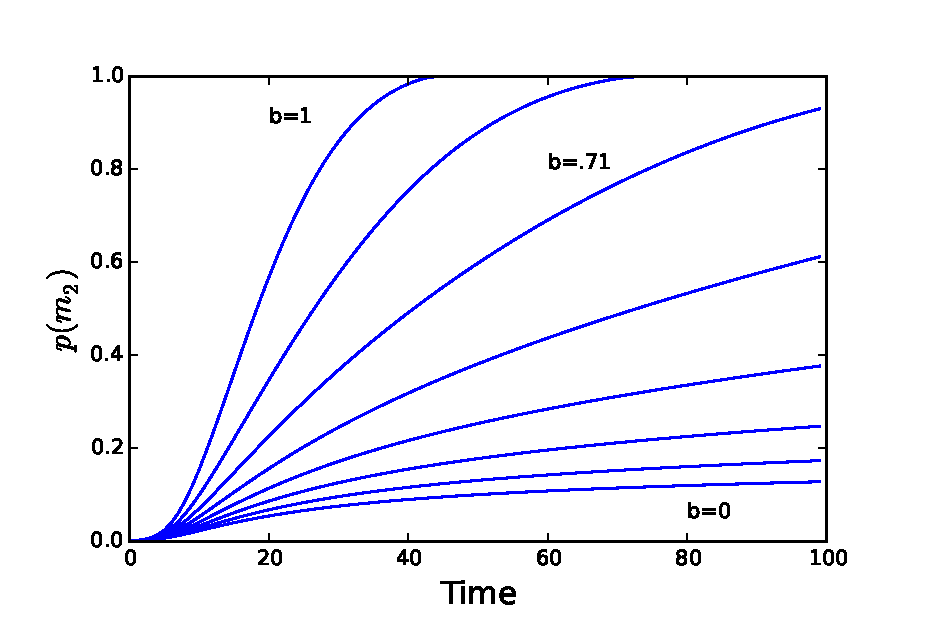
\includegraphics[width=.75\textwidth]{replicator-multiple-b.eps}
\caption{Proportion of $m_2$ under the discrete-time replicator dynamics for varying amounts of speaker bias}
\label{rd-multiple}
\end{figure}

So, our numerical simulations agree with the predictions from the static equilibrium analysis. If speaker bias is too large, then only a single form is used. More specifically, the form that is used at equilibrium is the form that started off restricted to higher degrees of activation. Now, while these simulations yield qualitative information about the dynamics of the functional cycle, we are interested in how this model can be used to understand the details of the functional cycle in the history of English. We now turn to fitting the model to historical trajectory of negation in English.


\section{Modeling the functional cycle}

Defining the stage game and the evolutionary dynamics allowed us to investigate the effect of speaker bias on the functional cycle in the abstract, but we are really interested in how the resulting model can be used to explain the actual historical trajectory of negation in a concrete case. In particular, we are interested in what happens when we fit the model to data from the history of negation in English. First, we describe the data that we fit the model to. Second, we define the parameters of the dynamics that we fit. Finally, we evaluate these parameters in light of the experimental data presented above.

The data we use are drawn from the PPCME2 \citep{ppcme2}. All tokens used are negative declaratives, excluding cases of contracted negation as well as cases that appear to be constituent negation.\footnote{We model the data used here after \cite{wallage2008}, which makes a compelling argument for treating contracted negation, among other cases, separately. Many thanks go to Aaron Ecay for sharing the code for generating the queries.} Each circle represents tokens in a given year. The size of the circle represents the number of tokens. The height of the circle represents the proportion of those instances that are a particular form. Locally-weighted regression lines are fit to these proportions. We see the transition from \textit{\color{red} ne} to \textit{\color{blue} ne...not} starting around the 12th century, followed closely by the transition from \textit{\color{blue} ne...not} to \textit{\color{green} not} in the 14th century.

\begin{figure}
\centering
     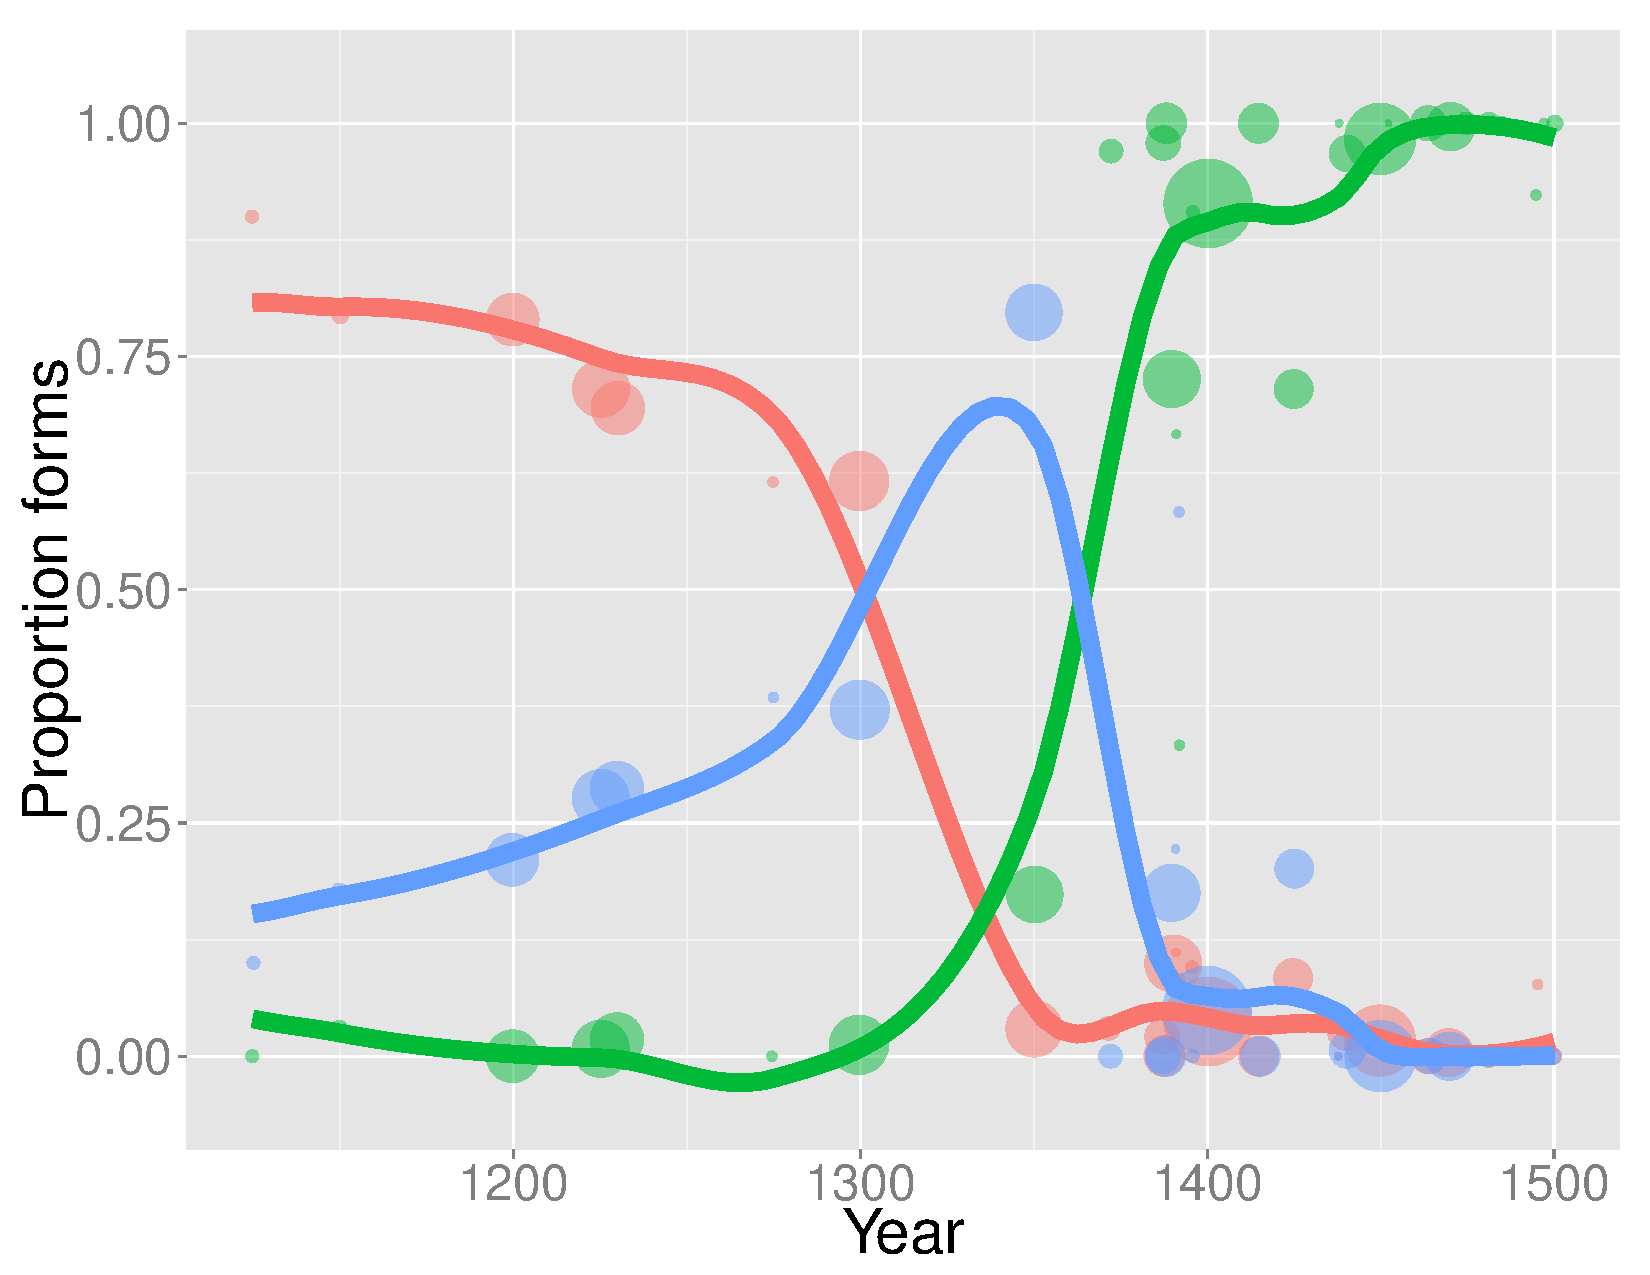
\includegraphics[width=.75\textwidth]{neg-year-lines.pdf}
\caption{Proportion of \textit{\color{red} ne}, \textit{\color{blue} ne...not}, and \textit{\color{green} not}  in Negative Declaratives}
\label{neg-three-plot}
\end{figure}

Now, given that we are interested in the functional cycle, we care about the transition from \textit{\color{red} ne} to \textit{\color{blue} ne...not}. That is, we care about an incoming emphatic form displacing an incumbent form. So, the subsequent rise of \textit{\color{green} not} is the second transition in the formal cycle, but not a part of the functional cycle. How should we deal with \textit{\color{green} not} in our analysis? There are two possibilities. First, we could ignore \textit{\color{green} not} and simply fit the model to the proportions of \textit{\color{red} ne} and \textit{\color{blue} ne...not}. The problem with doing so is that this attributes too much to small fluctuations in the proportions of \textit{\color{red} ne} and \textit{\color{blue} ne...not} even if those fluctuations are not meaningful in any sense relevant to the model. It is unlikely that small changes in the 15th century are something that we want to model.

Second, we could ignore the distinction between \textit{\color{blue} ne...not} and \textit{\color{green} not}, and treat them as if they were the same form. This alleviates the potential problem of attributing too much meaning to small fluctuations past a certain date. More importantly, it captures the contingency of the second transition of the formal cycle to purely post-verbal negation. That is, the rise of \textit{\color{green} not} is not a part of the functional cycle, nor is it a necessary and immediate consequence of the functional cycle. We only need to compare the history of negation in French where the embracing form goes to completion before being eventually replaced by the post-verbal form. Taking this route allows us apply the same model across languages without regard to subsequent contingent developments. The results of doing so are shown in Figure \ref{lump-plot1}.


\begin{figure}
\centering
     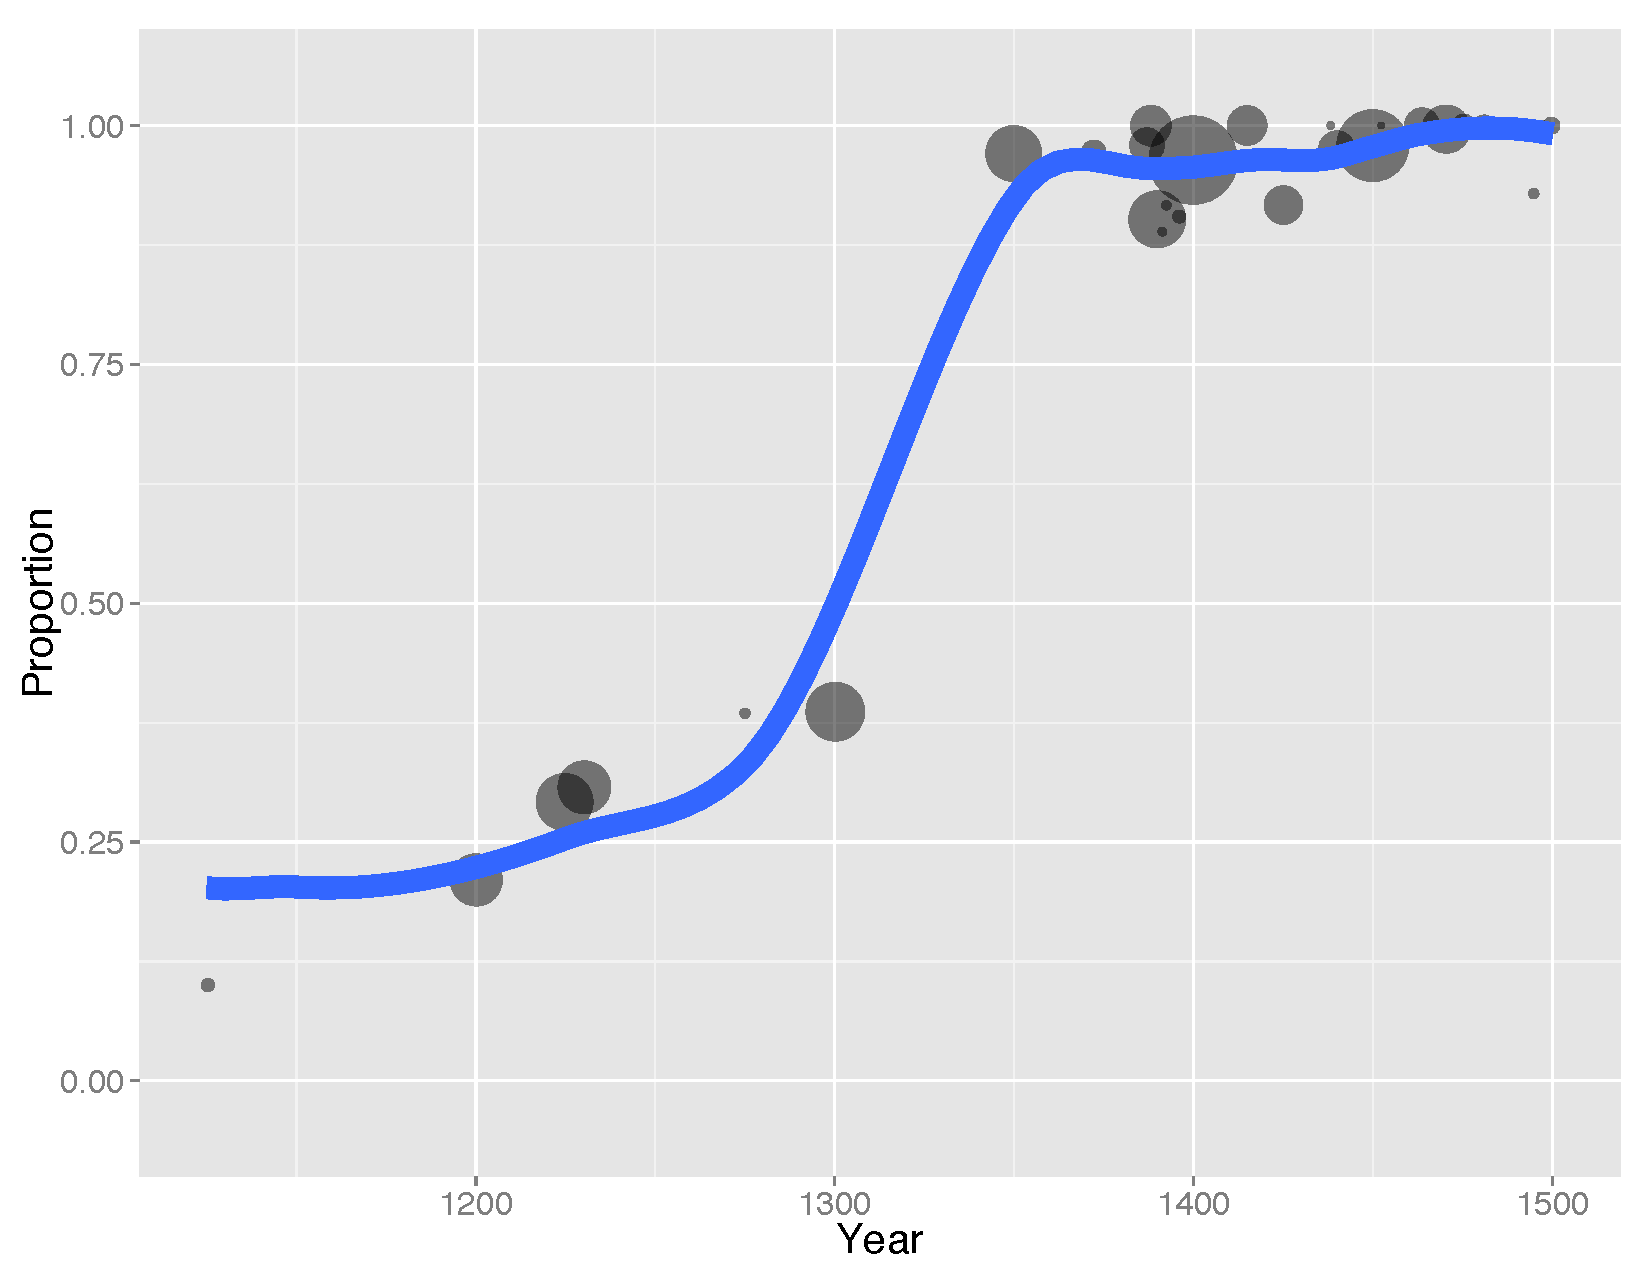
\includegraphics[width=.75\textwidth]{lump-plot1.pdf}
\caption{Proportion of \textit{\color{blue} ne...not} and \textit{\color{green} not}  versus  \textit{\color{red}  ne} over time}
\label{lump-plot1}
\end{figure}

Taking the trajectory of forms in Figure \ref{lump-plot1} as the data we want to fit our model to, we need to specify the parameters of the model to be fit. In particular, we need to define the initial state of how speakers use the different forms and how hearers respond to them. In fact, we have quite a bit of information regarding what the initial state of the functional cycle actually is. That is, we know that \textit{\color{blue} ne...not}   is fairly infrequent and largely restricted to high degrees of activation. Likewise, we know that hearers' response to \textit{\color{blue} ne...not}  is also largely restricted to actions corresponding to high degrees of activation. We can translate this information into conditions on the initial states of the speaker and hearer populations.

Regarding speakers we assume that both forms have a particular meaning, which is captured by conditional probability of states given a form. Namely, \textit{\color{red} ne} is the default form and does not carry any information above and beyond the prior, it roughly satisfies the following conditional distribution $p(t \mid \textcolor{red}{ne}) \sim \mathcal{B}(1, 2)$. In contrast, \textit{\color{blue} ne...not} is overwhelmingly used in states with high degrees of activation, that it satisfies the following conditional distribution $p(t \mid \textcolor{blue}{ne...not}) \sim \mathcal{B}(\alpha, 1)$. The larger $\alpha$ is, the more skewed towards high degrees of activation is \textit{\color{blue} ne...not}. Note that these two distributions along with the prior determine the initial proportion of \emph{\textcolor{blue}{ne...not}}. So, we only have a single parameter $\alpha$ to fit for the initial state of speakers.

%Moreover, if the initial proportion of the incoming form is sufficiently small then the incumbent form necessarily approximates the prior distribution.

Regarding hearers, we assume that the expected value of the responses to both forms correspond to the expected value of the conditional probability of states given the form. Intuitively, this corresponds to hearers starting off with a fairly accurate responses to the two forms. For \textit{\color{red} ne} this is satisfied by any distribution $\mathcal{B}(\alpha, \beta)$ such that $\alpha = \frac{1}{2}\beta$, which has an expected value $\frac{\frac{1}{2}\beta}{\frac{1}{2}\beta + \beta} = \frac{1}{3}$. Note that is the same as the expected value of the conditional probability of the state given the message $p(t \mid \textcolor{red}{ne}) \sim \mathcal{B}(1, 2)$.  So we take the conditional probability of actions given \textit{\color{red} ne}   to be $p(a \mid \textcolor{red}{ne}) \sim \mathcal{B}(\frac{1}{2}\beta_1, \beta_1)$. All that $\beta_1$ does is to determine how concentrated the action is around the expected value.  For \emph{\textcolor{blue}{ne...not}} let $\gamma = E[t \mid \textcolor{blue}{ne...not}]$, then this is satisfied by any distribution $\mathcal{B}(\alpha, \beta)$ such that $\alpha = \left( \frac{\gamma}{1 - \gamma} \right)\beta$, so we take the conditional probability of an action to be $p(a \mid \textcolor{blue}{ne...not}) \sim \mathcal{B}(\left( \frac{\gamma}{1 - \gamma} \right)\beta_2, \beta_2)$.  Again $\beta_2$ determines how concentrated the action is around the expected value. So, we have two parameters $\beta_1$ and $\beta_2$ to fit for the initial state of hearers.

The last thing to note before fitting the model is the notion of time. That is, the replicator dynamics specify how populations change from one point in time to the next, but how these abstract units correspond to days or years is unspecified. In what follows we treat each of these abstract time units as a year, but leave open the possibility that another proportion may be more appropriate. One option would be to treat the ratio between years and abstract time units as another parameter to be fit in the model, but for now we leave this as an avenue for future research.

We fit the initial state parameters and bias parameter to the data.\footnote{See Appendix B for the full details of the starting states and the resulting fit.} We begin by visualizing the overall trajectory of the incoming form, then turn to the change in the meaning of the two forms over time.  Figure \ref{m2-sol} shows the predicted proportion of \textit{\color{blue} ne...not} over historical time for the fitted model with the bias parameter $\hat{b} = 0.49132877$. Perhaps more importantly, we can actually inspect the inner workings of the model as they relate to the functional cycle.

\begin{figure}
\centering
     \includegraphics[width=.75\textwidth]{m2_sol.eps}
\caption{Predicted probability of \textit{\color{blue} ne...not} over time for fitted model of functional cycle.}
\label{m2-sol}
\end{figure}

In particular, we can examine how the information carried by the two forms changes over time. We gain insight into the functional cycle by considering how the meaning of \emph{\textcolor{blue}{ne...not}} changes over time as in Figure \ref{m2-meaning}. The horizontal axis represents states and vertical axis represents the conditional probability of states given that \emph{\textcolor{blue}{ne...not}} was used. We show this conditional probability at various points as the functional cycle proceeds. The dashed line indicates the prior probability distribution over states. The initial meaning of the incoming emphatic form is represented by the curve with the most rightwards skew. This indicates the point at which the incoming emphatic form carries the most information and is thus the most emphatic.  But, as time goes on, \emph{\textcolor{blue}{ne...not}} spreads to more and more degrees of activation as it the form increases in frequency. We represent this with subsequent distributions that move more and more towards the prior distribution. As they do so, the form loses its emphasis, as indicated by the thickness of the line. When \emph{\textcolor{blue}{ne...not}} is the only form, it carries no information about activation beyond the prior. Visually speaking, at this point its emphasis has faded entirely.


\begin{figure}
\centering
     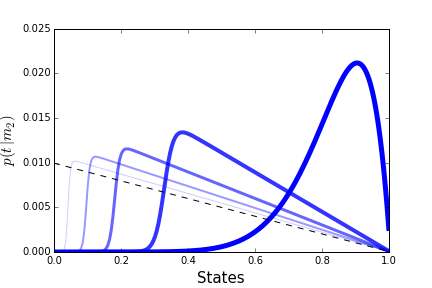
\includegraphics[width=.75\textwidth]{p_t_m2_rd.png}
\caption{The emphatic form over time as given by the conditional probability of states given \textit{\color{blue} ne...not}, where dashed line indicates prior probability distribution.}
\label{m2-meaning}
\end{figure}

We also gain insight in to the functional cycle by comparing the relative meaning of both forms. Comparing the meaning of \emph{\textcolor{red}{ne}} at the outset of the cycle and \emph{\textcolor{blue}{ne...not}} at the end of the cycle is particularly informative. Figure \ref{push-chain} emphatically demonstrates the dynamics of the push-chain scenario. At the beginning of the cycle in 1125 CE,  \emph{\textcolor{red}{ne}} carries no information about the degree of activation, it coincides with the prior as indicated by the dashed line.  In contrast, \emph{\textcolor{blue}{ne...not}} is overwhelmingly restricted to cases where the proposition being negated has a high degree of activation. Both of these facts are shown in the top panel of Figure \ref{push-chain}. But, one hundred years later, \emph{\textcolor{blue}{ne...not}} has expanded to more states as it increases in frequency and \emph{\textcolor{red}{ne}} is pushed to lower and lower degrees of activation. This is shown in the second panel of Figure \ref{push-chain}. As the functional cycle proceeds, the old form is pushed lower and lower down the scale. Eventually, the incoming form has displaced the incumbent form and ceases to carry any information about the degree of activation.

\begin{figure}
\centering
     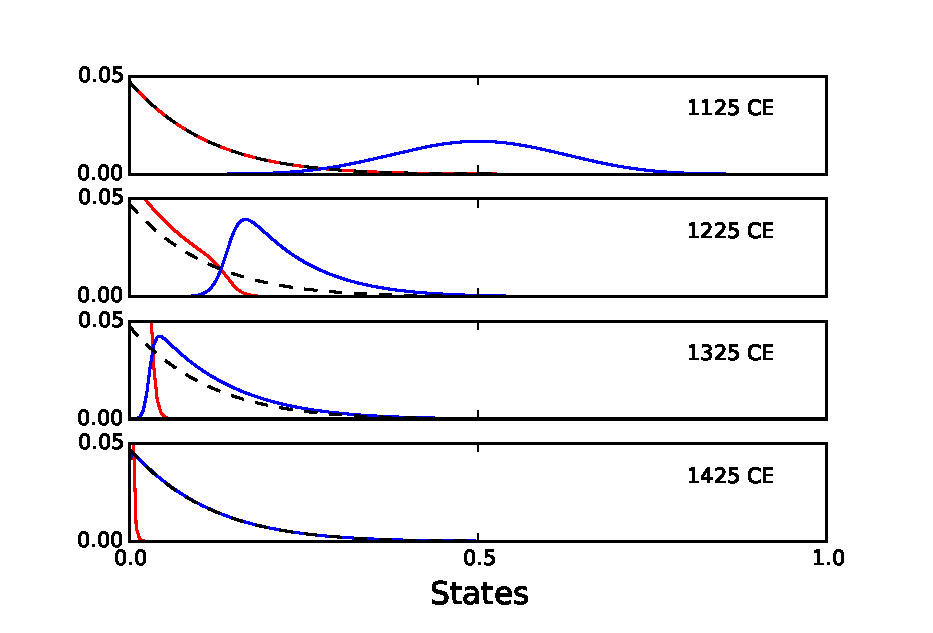
\includegraphics[width=\textwidth]{push_chain.eps}
\caption{The push-chain of the functional cycle given by the conditional probability of states given form at various points in time, where dashed line indicates prior probability.}
\label{push-chain}
\end{figure}

So, the dynamics of the fitted model match our theoretical conceptions of the functional cycle as a kind of push chain. The incoming form pushes the incumbent form out, eventually taking its place and losing its emphasis. Given that the driving force behind this change was posited to be speakers' bias to overestimate activation, it is important to take a moment to evaluate the value of the fitted bias parameter, $\hat{b}$. Given that the incoming form replaces the incumbent form, we would expect from our equilibrium analysis that at the very least $\hat{b} > \frac{1}{6}$, but this still leaves a fair amount of room for the parameter to vary. In fact the fitted value $\hat{b}=.4913287$ is well above this minimum. 

Now, given this value, we might ask whether it is reasonable in light of the experimental results discussed above. To evaluate the parameter, we return to the results reported in \cite{wu-keysar2007}. Namely, when playing a communication game, speakers relied on private knowledge of the names of shapes in a proportion of trials. We can use this information to estimate the expected value of the bias parameter exhibited by speakers in the experiment. 

To see this, first suppose that there are only two states corresponding to whether or not the name for a particular shape was learned privately or jointly. That is, knowing whether a name was learned privately or jointly is categorical. As \cite{heller-etal2012} found, this is a reasonable assumption given that participants were incredibly accurate at recalling the context of learning for shapes. Second, suppose that the utility functions for both speakers and hearers are the same form as above. Third, suppose that hearers take one action in response to names and another for descriptions that correspond to initial guesses about the status of the target shape. Then a speaker would only prefer the action taken in response to a name for a privately learned shape if $b > \frac{1}{2}$. 

But, this preferences is not categorical. In fact, from the experimental results we only know the probability that $b > \frac{1}{2}$. However, we can estimate the expected value of the bias parameter. Let $p(b) \sim \mathcal{B}(\alpha, \beta)$ be a distribution over the unit interval. We find the parameters such that $\int_\frac{1}{2}^1 p(b)db = p(b > \frac{1}{2})$, which in turn give the expected value of $b$. For example, where speakers use a privately known name in 5\% of trials $E[b] = .1398$, and where speakers use a privately known name in 28\% of trials $E[b] = .3549$.  

So, there are a range of potential values of speaker bias that we can estimate from the experimental evidence. In both cases these are smaller than the fitted value of the bias parameter for the functional cycle. However, there are good reasons to treat these experimental estimates as lower bounds. First, the fitted parameters deal with different domains. Where the experiments deal with the referential domain, the functional cycle deals with the propositional domain. It is certainly possible that speaker bias varies across these domains. In fact, we might even expect this. For example, referents often come along with some externally observable entity in the real world, whereas propositions often do not. The fact that propositions are in this sense more abstract may lead speakers to rely on their own perspective more.  Second, the experiments found speaker bias even between strangers. These kinds of communicative biases are even more pronounced between people who know each other well \citep{savitsky-etal:2011}.\footnote{For example, one day when I got home the first thing my wife said to me was, ``I \textsc{did} make an appointment.'' This struck me as out of the blue, but she said that she told me that she was feeling a little under the weather and debating whether her cold symptoms warranted a trip to the doctor. This conversation had happened several days prior and I had completely forgotten about it, but it was on her mind. In other words, her own subjective estimate of $p =$``I made a doctor's appointment.'' was greater than the actual degree of activation. In this case, I would say that the bias was fairly high $b \approx 1$.} Thus the degree of speaker bias in everyday life may be significantly larger than these experimental estimates suggest.

Careful experimentation will be needed to nail down how private and common knowledge are tracked in the propositional domain, and how this plays out in everyday life. However, the results are largely compatible with both the mechanics of the dynamic model of the functional cycle we have defined here.

\section*{Summary}

Separating out the formal and functional cycles lightens the explanatory burden. By isolating the functional cycle we were able to identify what conditions the incoming form and reason about why those conditioning factors change over time. In particular, we argued that speakers have difficulty in keeping track of private versus common knowledge, which biases them towards overestimating the activation of propositions being negated. The tools used to model the functional cycle allow us to offer the first explanatory model of the dynamics of how meaning changes over time.  Importantly, they also highlight the fact that while the driving force of the functional cycle is a byproduct of our cognitive limitations in tracking common knowledge, change comes about through the social interactions between individuals in a population.  Thus explaining the functional cycle requires a model of how pragmatic competence shapes signaling over time.

Before moving on, we pause to consider two potential lines of research related to the model we have discussed here. The first deals with the alternative definition of emphasis offered at the outset. That is, emphatic negation widens and strengthens negation to preclude exceptions. This interpretation is appealing insofar as negative polarity items are often recruited to create emphatic forms and have exactly this effect \citep{kadmon-landman1993any, eckardt2006}. However, this approach to the functional cycle would have to do two things. First, it would have to specify what serves the role of speaker bias in driving the increase of an incoming emphatic form. Second, it would have to address the problem of over-prediction. That is, if new signals can be formed with the addition of any negative polarity item, then there will always be new forms available, and thus the functional cycle should always be occurring. The fact that we do not observe Jespersen's treadmill means there must be some kind of restriction on what can serve as a new emphatic form. One potential restriction is that the new form must be free from sortal restrictions. For example, both ``I didn't move a crumb" and ``I didn't eat a crumb" must be equally acceptable.

The other line of research has to do with the implications of this model of the functional cycle for referring expressions that are also sensitive to degrees of activation. \cite{gundel-etal1993} refer to the scale of sensitivity as the \emph{giveness hierarchy}, which is roughly ordered by pronouns, demonstratives, definites, and indefinites. Pronouns are restricted to referring to entities that are directly activated, whereas indefinites can be used with any entity. Interestingly, similar diachronic patterns are observed as forms spread to lower degrees of activation. For example, the Modern English definite \emph{the} comes from the Old English demonstrative \emph{se}.\footnote{I cannot help but note discussions along this line with Jon Stevens (p.c. March 26, 2010):  ``One long term goal of this sort of research could be to connect it up with facts about language learning and pragmatics (perhaps using game theoretic tools) to paint a larger picture of why grammaticalization phenomena are so pervasive across languages.  As I alluded to in my vignette yesterday, a good model of semantic learning will likely interact with pragmatics in an interesting way; if such modeling techniques become sophisticated enough so as to model the acquisition of grammatical forms as well as content forms, then predictions will be made about the actuation and spread of bleaching, which could serve as a nice test of a model's plausibility."} However, there are at least two interesting implications of the model of the functional cycle for the stability within the givenness hierarchy. First, we would predict greater stability in these referential terms given the prior distribution over degrees of activation. If propositions are largely skewed towards being non-activated, then referents are largely skewed towards being activated. This change in the distribution largely counteracts any amount of speaker bias. Second, the generation of new pronouns, demonstratives, or definites is arguably a rare event. At least, it would seem rarer than a form of negation becoming associated with activation. We leave exploring both these lines of research for the future.


%\chapter{Cycles (30 pages)}
%\label{Cycles}
%
%\epigraph{"I don't know what you mean by 'glory,'?" Alice said.
%
%Humpty Dumpty smiled contemptuously. "Of course you don't -- till I tell you. I meant 'there's a nice knock-down argument for you!'?"
%
%"But 'glory' doesn't mean 'a nice knock-down argument'," Alice objected.
%
%"When I use a word," Humpty Dumpty said, in rather a scornful tone, "it means just what I choose it to mean -- neither more nor less."
%
%"The question is," said Alice, "whether you can make words mean so many different things."
%
%"The question is," said Humpty Dumpty, "which is to be masterÑthat's all."
%
%--Lewis Carroll\\
%
%I canÕt say `ItÕs cold here' and mean `ItÕs warm here' -- at least, not without a little help from my friends.\\--David Lewis}
%
%
%We are now in a position to bring the formal framework developed in Section \ref{Signaling} to bear on the use of emphatic negation and its role in Jespersen's Cycle. We begin by first mapping the components discussed in Section \ref{Background} onto the structure of a signaling game. The possibility of different preferences for speakers and hearers is incorporated into the structure of the model. We determine the existence of evolutionarily stable strategies and note the transfer of information as the interests of speaker and hearer diverge. As the preferences of speakers and hearers diverge signaling becomes less informative. For sufficiently low differences, signaling remains informative, but beyond a certain point signaling collapses into uninformative pooling. We then consider the impact of introducing new signals, which lead to a kind of push-chain where the least informative signal is lost. Throughout, we discuss the implications of the model for Jespersen's Cycle.
%
%\section{Signaling Game}
%
%To begin, we must first consider how signaling games capture the use of negation. As we noted above, the difference between plain and emphatic negation is captured by the standard of precision applied. The speaker has knowledge about some state of the world which renders a particular negative expression acceptable on some standards, but not necessarily on others. Thus, there exists a continuum of states for the speaker, which we will take to be the interval $T = [0,1]$. The lowest possible value on such an interval corresponds to the weakest possible standard of precision that would still render the negative expression acceptable.\footnote{Here we leave out the possibility of the use of a given expression in the absence of any standard of precision being met. That is, we leave out cases of outright lying. Such cases are particularly interesting, but we leave them as a consideration for future study.} The highest possible value on the interval is then the strictest possible standard of 
%interpretation available. 
%
%Given that the speaker has observed some state of affairs, $t \in T$, he must choose a message, $m \in M$, to send to the hearer. Let $\mathcal{P}_n(T)= 0 < ... < t_{n-1} < ... < 1$ be a partition of the state space into $n$ subintervals.  A speaker's strategy is then a function from a partition of the type space to messages, $S : [\mathcal{P}_n(T) \rightarrow M]$. Intuitively, this is simply a way of carving up the state space into discrete regions and using those regions to determine which signal to send. For example, the trivial partition, $\mathcal{P}_1(T)$, occurs when the sender pools all types together and uses only a single message. In what follows we will largely be concerned with partitions of at least size two $\mathcal{P}_2(T)$. For example, consider the case of two messages, consisting of just a plain and an emphatic form. Letting $\mathcal{P}_2(T) = 0 < t_1 < 1$, a possible sender strategy is then  $s(t) = m_1$ for $t \in (0,t_1)$, and $s(t) = m_2$ for $t \in (t_1,1)$. That is, the sender uses 
%$m_1$ for all types in the first subinterval, and $m_2$ for the second subinterval. Intuitively, we would refer to $m_1$ as the plain form of negation and $m_2$ as the emphatic.
%
%Once the speaker has sent a message, the hearer is faced with the problem of how to interpret it. Given that the hearer cannot read the speaker's mind, she must infer the state of affairs that prompted the use of a particular form. That is, given the information conveyed by the signal, she must do her best to determine the standard of precision that warrants the speakers assertion. We will take the space of possible interpretations available to the hearer to be equivalent to the type space of the speaker, $A = [0,1]$. This representation captures the fact that the interpretation of expressions is not an all or nothing affair, but rather a matter of degrees.  A hearer's strategy is then a mapping from messages to interpretations, as above, $R : [M \rightarrow A]$.
%
%
%\begin{figure}
%\begin{center}
%\begin{tikzpicture}[->,>=stealth',shorten >=1pt,auto,node distance=3cm]
%  \node (A)      {$t_0$};
%  \node (B) [right of=A]  {$m_0$};
%  \node (C) [right of=B] {$a_0$};
%  \node (D) [below of=A] {$t_1$};
%  \node (E) [right of=D] {$m_1$};
%  \node (F) [right of=E] {$a_1$};
%\path[->] (A) edge node {$s_0^0$} (B)
%	  (A) edge[dashed,pos=0.85] node {$s_0^1$} (E)
%	  (B) edge node {$r_0^0$} (C)
%	  (B) edge[dashed,pos=0.85] node {$r_0^1$} (F)
%	  (D) edge[below] node {$s_1^1$} (E)
%	  (D) edge[dashed,pos=0.75] node {$s_1^0$} (B)
%	  (E) edge[below] node {$r_1^1$} (F)
%	  (E) edge[dashed,pos=0.75] node {$r_1^0$} (C);
%\end{tikzpicture}
%\end{center}
%\caption{Probabilities of actions in signaling game}
%\label{probs}
%\end{figure}
%
%\begin{figure}
%\begin{center}
%\begin{tikzpicture}[->,>=stealth',shorten >=1pt,auto,node distance=3cm]
%  \node (A)      {$t_0$};
%  \node (B) [right of=A]  {$m_0$};
%  \node (C) [right of=B] {$a_0$};
%  \node (D) [below of=A] {$t_1$};
%  \node (E) [right of=D] {$m_1$};
%  \node (F) [right of=E] {$a_1$};
%%  \node (G) [below of=D] {$t_2$};
%\path[->] (A) edge node {$s_0^0$} (B)
%	  (A) edge[dashed,pos=0.85] node {$s_0^1$} (E)
%	  (B) edge node {$r_0^0$} (C)
%	  (B) edge[dashed,pos=0.85] node {$r_0^1$} (F)
%	  (D) edge[below] node {$s_1^1$} (E)
%	  (D) edge[dashed,pos=0.75] node {$s_1^0$} (B)
%	  (E) edge[below] node {$r_1^1$} (F)
%	  (E) edge[dashed,pos=0.75] node {$r_1^0$} (C);
%\end{tikzpicture}
%\end{center}
%\caption{Probabilities of actions in signaling game}
%%\label{probs}
%\end{figure}
%
%
%
%With the definition of the strategies available to speakers and hearers, we can ask what kinds of preferences both might have over the correspondence between actual and inferred standards. It is uncontroversial that hearers are in the business of doing their best to accurately infer the actual state of affairs that prompted the signal. That is, hearers prefer their interpretation to be as close as possible to the standard of precision that the speaker actually has evidence for.  If it were otherwise, the existence of language would be truly puzzling from an evolutionary perspective; the gullible are not long for the tooth and claw world. So, if hearers are interested in the accurate transmission of information, then any misalignment must come from speakers' preferences. 
%
%From the perspective of the speaker, we can adduce at least two related reasons why speakers might prefer overestimation. The first imputes a kind of categorical bias on the part of speakers, whereas the second relaxes this bias towards reasonability. We address them each in turn. First, we consider what the goals of communication are. Arguably, our chief goal in uttering a given expression is to affect some response in our interlocutors. In the case of a declaration we might think of this in terms of how convinced the hearer is after hearing an utterance. Or, in the terms we have developed thus far, we want the hearer to infer a particular standard of precision. We could take this preference as categorical. Namely, that regardless of the actual standard of precision, speakers want hearers to infer the absolute highest standard of precision possible. Given such a preference and a choice between signals that hearers respond to differentially, speakers will always choose the form that elicits the higher 
%standard.  Speakers are, so to speak, on the lookout for the form that gives them the most bang for their breath. It should be noted that this bias is stipulative only insofar as it arises from the fundamental way we use words to do things.
%
%Second, while this bias may naturally exist, it need not be categorical. Rather, speakers may simply prefer that hearers infer a standard of precision that is at least is strict as their own. This can be taken as a natural corollary of the inferential nature of communication. Hearers cannot read minds, and thus they must make some inference about the actual standard of precision. Speakers have only an indirect influence on this process of inference. Thus, they may wish to hedge their bets in a particular direction. Namely, they may want the inferred standard to be at least as strict as there own because it ensures that their own beliefs stand in a particular relation to hearers'. That is, the hearer's beliefs probabilistically entail those of the speaker.
%
%The impact of this relationship is particularly clear with regard to perlocutionary concerns. For example, imagine the case where the issuer of one of the following threats has absolutely no desire to follow through on it.
%
%  \ex. \a. If you move, I'll shoot.
%       \b. If you budge an inch, I'll shoot.
%
%By using the stronger threat, leading the hearer to infer a stricter standard than actually holds, the speaker has a better chance of not being forced to follow through on it. That is, the hearer will restrict his actions to those that do not constitute movement at the stricter standard, thus guaranteeing that they will not at the weaker actual standard. 
%
%The same concerns hold in far more magnanimous circumstances. For example, in the case of offering a friend genuine advice on dining options, one might deem a mediocre restaurant one of the following.
%
% \ex. \a. Not good.
%      \b. Not worth a cent!
%
%While clearly hyperbole, the latter, much like the strong threat, offers a means for speakers to guide a friend to a good meal. In both cases, when hearers underestimate the standard of precision, the speaker runs the risk of not achieving his goals with resulting dire or not so delicious consequences. In contrast, these goals are guaranteed when hearers overestimate the standard of precision.
%
%We can encode this slight bias in the utility functions of senders and receivers. As a means of parameterizing this possibility, we define the sender and receiver utility functions as a pair of quadratic functions, as in \cite{crawford-sobel:1982}, where $b \in [0,1]$ reflects the bias of the sender.\footnote{This bias need not be constant. For example, we might suppose that the bias is uniformly distributed over the interval $(t,t+b)$. This would capture the intuition that some of the time a speaker prefers overestimation of the standard, but not others. All of the following result hold for this more general case. As a preview, the only change below is that partial pooling equilibrium is defined at $t^* = \frac{1}{2} - 3b$ }
%
%\begin{equation}
%\begin{split}
%     U_S(t, a) &= -(a - t - b)^2\\
%  	 U_R(t, a) &= -(a - t)^2
%\end{split}
%\end{equation}
%These utility functions reflect two intuitions. First, for a given type of sender, there is an action that maximizes the receiver's payoff. That is, the receiver does best by taking the action that is closest to the sender's type. Second, for a sender with a particular type, the action that maximizes the sender's payoff is offset by some bias, $b$. That is, the sender prefers the receiver to take the action she thinks appropriate for some higher type. In this case, $b$ represents the degree to which the sender wishes to exaggerate his type, if the receiver believes such exaggerations. When $b=0$ the interests of senders and receivers are completely aligned, but as $b$ grows, they diverge. This parallels the intuition that hearers are trying to infer the standard of precision for a given assertion, and prefer this to be as accurate as possible. It also reflects the fact that speakers have a slight preference for hearers to overestimate the standard of precision.
%
%The impact of the sender's bias can be visualized as in Figure \ref{receiver_payoff}. For a sender with information $t=0$, the receiver would do best to take the action that accurately picks out the sender's state. In contrast, the sender's most preferred action is offset by the amount of bias. In the case where $b=\frac{1}{2}$, then the sender prefers the speaker to take an action higher than the receiver would prefer. This mismatch is only exacerbated as the amount of bias increases, as can be seen for the case where $b=1$. Visually speaking, as the bias increases, the utility functions of the sender and the receiver move away from each other. 
%
%
%\begin{figure}
%\begin{center}
%\begin{tikzpicture}
%\node (left) at (-1, 2)    {
\includegraphics[width=.15\textwidth]{left.jpg}};
%%draw horizontal line
%\draw (0,0) -- (6,0);
%%draw ticks
%\draw (0,3pt) -- (0,-3pt);
%\draw (6,3pt) -- (6,-3pt);
%%draw tick labels
%\draw (0,0) node[below=3pt] {\textsc{discourse new} } ;
%\draw (6,0) node[below=3pt] {\textsc{discourse old} } ;
%%
%\draw (3,3pt) -- (3,-3pt);
%\node (state) at (3, 1)    {$t$};
%%
%\draw (5,3pt) -- (5,-3pt);
%\node (state) at (5, 1)    {$t+b$};
%\draw [ultra thick] (3,1.5) to (5,1.5);
%\node (state) at (4, 1.75)    {$b$};
%\end{tikzpicture}     
%\end{center}
%\caption{$p :$ The plumber came.}
%\end{figure}
%
%\section{Equilibria}
%
%For a given pair of sender and receiver strategies we can calculate the expected utility. In what follows we will assume that types are uniformly distributed over the interval, which yields the following expected utilities. Note that these are exactly parallel to expected utilities in a discrete state space presented above.
%
%\begin{equation}
%\begin{split}
%     E[U_S(s, r)] &= \int_T -(r(s(t)) - t - b)^2 dt\\
%      E[U_R(s, r)] &= \int_T -(r(s(t)) - t)^2 dt
%\end{split}
%\end{equation}
%
%Now, we want to determine the conditions for equilibria. By doing so, we are determining what kinds of behavior we would expect on the part of speakers and hearers given the speaker's bias. That is, we want know how speakers will use different forms to signal standards of precision and how hearers will interpret them. The existence of different equilibria and their relative stability are crucial to the dynamics of Jespersen's Cycle.
%
%Consider the potential equilibrium strategy profile $\langle s^*, r^* \rangle$. Let $s^*$ induce a partition of type $\mathcal{P}_2(T)$, where $t^*$ is the relevant threshold that distinguishes the two messages. Let $s^*(t) = m_1$ for $t \in (0,t^*)$ and $s^*(t) = m_2$ for $t \in (t^*,1)$. Let $r^*(m_1) = a_1^*$ and $r^*(m_2) = a_2^*$. In words, the sender splits the type space in two and sends a unique message for each subinterval. These are the plain and the emphatic forms of negation, respectively. The receiver responds to these messages with a particular action.  These are the inferred standards of precision in response to the different forms.
%
%The strategy profile is an equilibrium if the relevant strategies are joint best responses. We can determine this by simply taking the partial derivative of the relevant utility functions with regard to the relevant variables. For the receiver, this can be determined by considering what actions are the best response to the senders partition. This simply tells us how the receiver's inference depends on the sender's use of the different forms.
%
%\begin{equation}
%\frac{\partial}{\partial a_1^*}E[U_R(s, r)] = \frac{\partial}{\partial a_2^*}E[U_R(s, r)] = 0
%\end{equation}
%These values are uniquely satisfied when the following hold.
%
%\begin{equation}
%     \begin{split}
%	  a_1^* &= \frac{t^*}{2}\\
%	  a_2^* &= \frac{1 + t^*}{2}
%     \end{split}
%\end{equation}
%Intuitively, this means that however the speaker splits up the standards of precision, the receiver should respond to the emphatic form by inferring a higher standard of precision and the plain form with a lower standard of precision. The exact placement of these responses is determined by how the sender uses the signals. Namely, the hearer should infer the average standard of precision used for each of the two forms.
%
%For the sender, we can proceed in a similar fashion determining when the following holds.
%\begin{equation}
% \frac{\partial}{\partial t^*}E[U_S(s, r)] = 0
%\end{equation}
%This equation is satisfied when one of the following holds.
%
%\begin{equation}
%     \begin{split}
% 	t^* &= 0\\
%	t^* &= \frac{3}{4}(a_1^* + a_2^*) - \frac{3}{2}b - \frac{1}{4}\\
%	t^* &= 1
%     \end{split}
%\end{equation}
%
%These constraints together give rise to three distinct systems of equation. Solving each for $t^*$, we find the following equilibrium solutions in terms of the bias of the sender.
%
%\begin{equation}
%\begin{split}
%     t^* &= 0\\
%     t^* &= \frac{1}{2} - 6b\\
%     t^* &= 1
%\end{split}
%\end{equation}
%Both the first and the last of these equilibria are pooling equilibria. That is, senders only ever use a single signal. In response to this, receivers take the action that maximizes their expected utility given the prior probability distribution over types. That is, they guess the expected value of the type space. They simply infer the average standard of precision.
%
%In contrast, the middle equilibrium constitutes a partially separating equilibrium. It is only partially separating because the state space is infinite, while the message space is not. This means that every type cannot be fully revealed, but that some information is transferred. The amount of information transferred and the distinction between the partially separating and pooling equilibria can be characterized in information-theoretic terms \citep{shannon:1948}. In particular, we can think of the amount of information conveyed by a particular signal at equilibrium according to the \emph{Kullback-Leibler Divergence} \citeyearpar{kullback-leibler1951divergence}.
%
%\begin{equation}
%     D_{KL}(P || Q) = \int_{-\infty}^{\infty} log\left( \frac{p(x)}{q(x)}  \right)p(x) dx
%\end{equation}
%This serves as a measure for how much change is induced in the receiver by a particular message. That is, in our case $q(x)$ corresponds to the prior probability distribution over types, and $p(x)$ corresponds to the probability of a sender being of a particular type given the message. The more the message shifts the probability from the prior, the more information it conveys. And, the less a message shifts the probability from the prior, the less information it conveys. 
%
%For example, taking either of the pooling equilibria as an example.  If senders use the same signal regardless of state, then the conditional probability is the same as the prior probability. This means that there is absolutely no change from the prior probability, and hence zero information is transmitted via the signal. In contrast, for any partially separating equilibrium, a particular message induces a shift from the prior probability, and thus conveys some information. We should note that the amount of information conveyed regarding the standard of precision is distinct from the propositional content of a given utterance. For example, in the case where speakers use only a single form of negation for all standards of precision, the hearer will have no information in addition to and exceeding the prior probability. However, she will know the propositional content of the utterance. In other words, she will know \emph{that} negation was used, but not \emph{how} it was used.
%
%
%Information is transferred at equilibrium only if the partially separating equilibrium exists. This is the case when the sender's bias is sufficiently low. Namely, only if $b < \frac{1}{12}$. If the bias is too large, then the partially separating equilibrium collapses into the lower pooling equilibrium.  However, a partially separating equilibrium, if it exists, is the only evolutionarily stable strategy profile. To see this note that in any pooling equilibrium receivers can respond to an unused message with any action whatsoever without affecting their expected utility. This means that pooling equilibria are not strict Nash equilibria and are thus not stable to invasion or innovation. 
%
%% For example, suppose that receivers responded to an unused message with an action $a > \frac{1}{2}$. All senders would then do better to use that previously unused message in a particular set of states, $(\frac{1}{2}(a + \frac{1}{2}), 1]$. In turn, receivers woul
%% 
%%  have an incentive to adjust their responses to the two messages. In turn, senders have an incentive to adjust to this adjustment, and so forth. This process of mutual adjustment ends at the evolutionarily stable partially separating equilibrium.
%
%We have established an upper limit on the amount of bias that allows for two signals to be used informatively. If this bias is exceeded, then signaling collapses. A single message is used, but carries no information. In fact, for a given number of signals, $n$, there exists some level of bias, $b_n$, that allows for their informative use in a partially separating equilibrium based on a sender's partition of the type space, $\mathcal{P}_n$ \citep{crawford-sobel:1982}. As the number of signals increase, the amount of bias must decrease to allow for informativity, thus $b_2 > b_3 > ... > b_n$. Intuitively, as the preferences of senders and receivers approach each other a finer and finer partition of the space is possible.
%
%\section{Dynamics}
%
%So, what does this mean for Jespersen's cycle? Intuitively, the pragmatics of emphasis suggest that the population originally starts at a point where one form is used with a  very high standard of precision and another is used for all other standards. That is, emphatic negation is distinguished from plain negation in its contexts of use. We can determine what will happen to these two signals over time. Intuitively, under the game dynamics, the signals will converge to their equilibrium use.
%
%Under the game dynamics, for any amount of bias, no matter how slight, the emphatic form will spread to lower and lower standards of precision until it reaches its equilibrium use. The amount of bias determines where this process stops. That is, if a partially separating equilibrium exists, then the emphatic form will expand to encompass all standards of the upper part of the partition. In other words, the emphatic will be \emph{attenuated}, but still carry some information.  If no separation is possible, the emphatic form will spread across all standards. In other words, the emphatic will be entirely \emph{bleached} of its emphasis. Note that in both cases the process can be characterized in information-theoretic terms. That is, as the emphatic form spreads to more and more standard it conveys less and less information. 
%
%The stable coexistence of plain and emphatic negation for long periods of time suggest that the bias is sufficiently small to allow for at least two forms. This, however, raises the question of what destabilizes the system. The system must be disturbed by a push chain, whereby the signal used for the lowest subinterval is lost. More generally, imagine a system with bias $b_n$ at equilibrium. Now, suppose that a new signal is introduced, so that there are now $n+1$ signals. Clearly, the system is not stable. However, it will be carried back to some equilibrium by the game dynamics. The resultant equilibrium depends on the character of the signal that is introduced. Let $a'$ be the response of receivers to the new signal $m'$. All messages that receive a lower response than $a'$ will be pushed down, the lowest of these being pushed out of use completely.  In the case of Jespersen's Cycle, new signals enter with a high $a'$, and thus displace everything below. That is, they are emphatic and lead hearers to 
%infer a high standard of precision. This means that all other forms lower in the scale will be pushed down and the lowest will be pushed out of existence, exactly like what we see in the actual instantiation of the cycle.
%
%
%The motivation of this project stems from particular hypotheses about the conditioning factors of negation in Jespersen's Cycle \citeyearpar{jespersen:1917}, which can be characterized by the transition from pre-verbal to embracing to post-verbal negation: \textsc{\color{red} neg V} $\rightarrow$ \textsc{\color{blue} neg V neg} $\rightarrow$ \textsc{\color{green} V neg}. In particular, \cite{hansen2009, hansen-visconti2009,hansen-visconti2012} have used historical corpora of French and Italian to show that the embracing form (\textsc{\color{blue} neg V neg}) is sensitive to the discourse status of the proposition being negated. Namely, the embracing form is restricted to instances where the proposition being negated is either \textsc{discourse old} or \textsc{inferrable}.
%
%\cite{schwenter2005,schwenter2006} uses synchronic data from Brazilian Portuguese to demonstrate the sensitivity of negation to these distinctions. Consider the following scenario. Suppose that a husband and wife expect a plumber to come fix their leaky faucet while they are at work during the day. The husband arrives home before his wife to find a still leaky faucet. The wife arrives home shortly and the first thing her husband says is the following.
%
%\exg.  O bombeiro \textsc{\color{red} n{\~a}o} \textsc{\color{red} Veio}.\\
%         The plumber neg came\\
%         ``The plumber didn't come."\\
%
%\exg. \#O bombeiro \textsc{\color{blue}n{\~a}o} \textsc{\color{blue}Veio} \textsc{\color{blue}n{\~a}o}.\\
%	The plumber neg came neg\\
%	``The plumber didn't come."\\
%
%The reason that the embracing form is odd is that it comes out of the blue, so to speak. That is, the proposition ``The plumber came.'' is entirely \textsc{discourse new}. Even if the husband has some expectation that his wife has been thinking about whether or not the plumber came, the proposition has not been introduced into the \emph{discourse} yet. The embracing form cannot be used to negate \textsc{discourse new} propositions.
%
%However, how the proposition can be introduced into the discourse in several ways, both explicitly and implicitly. For example, if the wife walks in the door and says the following.
%
%\exg.  O bombeiro veio hoje?\\
%       The plumber came today\\
%         ``Did the plumber come today?"\\
%
%Asking the question has explicitly introduced the proposition into the discourse, making either form appropriate in the husband's response. In fact, the wife need not even explicitly ask the question. For example, if she arrives home and points quizzically at sink, then the embracing form is fine. This is because the proposition can be inferred from the discourse.
%
%Schwenter shows that even finer distinctions can be made in the sensitivity of different forms of negation to discourse context. For example, consider the following scenario. Suppose that two colleagues meet in a departmental hallway in the afternoon after a scheduled talk, and one asks the other the following question.
%
%\exg. Voc{\^e} gostou da palestra da Maria?\\
%	 you liked the talk of Maria\\
%	 ``Did you like Maria's talk?"
%
%\exg. \textsc{\color{blue}N{\~a}o} \textsc{\color{blue}Fui} \textsc{\color{blue}n{\~a}o}.\\
%	 neg went neg\\
%	 ``I didn't go."\\
%
%\exg. \#\textsc{\color{green}Fui} \textsc{\color{green}n{\~a}o}.\\
%	  went neg\\
%	 ``I didn't go."\\
%
%The reason that the post-verbal form is odd is that the proposition being negated ``I went (to Maria's talk).'' is only indirectly connected to the discourse. That is, liking a talk presumably requires having attended it, so the proposition is only \textsc{inferrable} from the discourse. The post-verbal form cannot be used where the proposition is discourse new or inferrable. This is made clear by altering the form of the response to the question of liking the talk.
%
%\exg. \textsc{\color{blue}N{\~a}o} \textsc{\color{blue}Gostei} \textsc{\color{blue}n{\~a}o}.\\
%	 neg liked neg\\
%	 ``I didn't like it."\\
%
%\exg. \textsc{\color{green}Gostei} \textsc{\color{green}n{\~a}o}.\\
%	  liked neg\\
%	 ``I didn't like it."\\
%
%In this case the post-verbal form is acceptable because the proposition ``I liked Maria's talk.'' has been introduced into the discourse by the original question. The conditions and restrictions on different forms can be summarized as in Table \ref{schwenter}. The pre-verbal form is acceptable in any context, but the other two forms are only acceptable in more and more restricted contexts,
%
%\begin{table}
%\begin{center}
%\begin{tabular}{@{}ccccc@{}}
%      \hline
%       & \textsc{discourse new} & \textsc{inferrable} & \textsc{discourse old}\\ \hline
%      \textsc{\color{red} neg V} & $\checkmark$ &  $\checkmark$ &  $\checkmark$ \\
%      \textsc{\color{blue} neg V neg} & \#  & $\checkmark$ & $\checkmark$ \\
%      \textsc{\color{green} V neg} & \#  & \#  & $\checkmark$ \\
%      \hline
%\end{tabular}     
%\end{center}
%\caption{Acceptability of forms in discourse contexts}     
%\label{schwenter}
%\end{table}
%
%
%It is not entirely clear if the forms of negation in Brazilian Portuguese should be treated differently than the canonical cases of embracing negation in Jespersen's Cycle (cf. \emph{ne...pas} in French, \emph{ne...not} in English). However, languages with only the pre-verbal and embracing form have been shown to exhibit this same sensitivity to discourse status (e.g. \cite{schwenter2006} for Catalan and Italian, \cite{hansen2009} for French). Namely, languages that only have two forms make the distinction between \textsc{discourse new} and everything else. This, of course raises the question of whether the post-verbal form is necessarily sensitive to discourse status or is the result of other processes, such as phonetic reduction. These are open empirical questions, which might also vary by the particular circumstances of a language.
%
%However, the general shape of the conditioning factors suggests an intuitive characterization Jespersen's Cycle. That is, the different forms of negation are sensitive to the scale of how closely the negated proposition is connected to the discourse. That is, if we take connection to the discourse as a continuous measure, then discourse new propositions are at the low end, discourse old propositions are at the high end, and inferrable propositions are somewhere in the middle. In fact, we can simply reduce this to a scale of degrees of inferrability: discourse new propositions are not inferrable since we can't read minds, and discourse old propositions are completely inferrable since they have just been explicitly introduced into the discourse. 
%
%We can represent this visually as in Figure \ref{continuum}, where we have simply taken the discrete categories used to construct Table \ref{schwenter} and treated them as a continuum. In fact, this wording is potentially misleading. If discourse status is about beliefs, then the underlying phenomenon is essentially gradient in nature. The discrete categories are useful because they correspond to portions of the continuum. While we have robust intuitions about the discrete categories, the varying strength of these intuitions suggests that the underlying phenomenon is essentially gradient in nature.
%
%\begin{figure}
%     \begin{center}
%\begin{tikzpicture}
%% \node (left) at (-1, 2)    {
\includegraphics[width=.15\textwidth]{left.jpg}};
%% \node (left) at (7, 2)    {
\includegraphics[width=.15\textwidth]{right.jpg}};
%%draw horizontal line
%\draw (0,0) -- (6,0);
%%draw ticks
%\draw (0,3pt) -- (0,-3pt);
%\draw (6,3pt) -- (6,-3pt);
%%draw tick labels
%\draw (0,0) node[below=3pt] {0} ;
%\draw (6,0) node[below=3pt] {1} ;
%\draw (0,-.5) node[below=3pt] {\textsc{discourse new} } ;
%\draw (6,-.5) node[below=3pt] {\textsc{discourse old} } ;
%%
%\draw [ultra thick,red] (0,1.5) to (6,1.5);
%\draw [ultra thick,blue] (2,.5) to (6,.5);
%\draw (3,2) node {\textsc{\color{red} neg V}};
%\draw (4,1) node {\textsc{\color{blue} neg V neg}};
%% \draw (2,.25) node {$a_{\text{\textsc{\color{red} neg V}}}$};
%% \draw (5,.25) node {$a_{\textsc{\color{blue} neg V neg}}$};
%
%\end{tikzpicture}     
%\end{center}
%  \caption{Forms of negation given degree of inferrability}
%  \label{continuum}
%\end{figure}
%
%
%
%The continuous representation also offers us some insight into \emph{why} Jespersen's Cycle occurs. The reasoning is as follows. First, keeping track of what is actually part of the discourse is difficult. In fact, this is the problem of \emph{common knowledge}\footnote{In epistemic logic \emph{mutual knowledge} only requires that everyone know that $p$, without any further steps. Thus anything that is common knowledge is also mutual knowledge, but not \emph{vice versa}. \cite{lewis:1969} introduced common knowledge in Philosophy. \cite{clark-marshall1981} use the term ``mutual knowledge'' to refer to common knowledge.}, that everyone knows that $p$, that everyone knows that everyone knows that $p$, \emph{ad infinitum}. \cite{clark-marshall1981} outline a set of reasonable heuristics for circumventing this infinite regress, including physical or linguistic co-presence and community membership. While these heuristics are made with reference to resolving the problem of common knowledge, they extend equally to 
%propositions. Namely, propositions can be introduced to the discourse either explicitly (linguistic co-presence) or implicitly (physical co-presence, community membership).
%
%Second, we have ample experimental evidence that speakers have particular biases in communication. Speakers tend to overestimate how successful they are at communication. \cite{savitsky-etal:2011} had two pairs of friends participate in a simple communication task. All four participants sat back to back and were individually given lists of four-way ambiguous sentences to read out loud with a specified meaning. For example, the sentence ``It's getting hot in here.'' could be interpreted as an indirect request to open the window or an amorous advance. Participants were asked to do two things. They were asked to guess the intended meaning of the sentences spoken by the other participants. They were also asked to estimate how many of the sentences the friend they came with had guessed correctly, and how many sentences the strangers from the other pair had guessed correctly. 
%
%The results can be seen in Figure \ref{savitsky}. Listeners were reliably above chance at guessing the intended meaning out of the four potential meanings, but, friends and strangers did not differ significantly. However, speakers had much higher expectations  for listeners, significantly overestimating how many sentences listeners would accurately guess. This suggests that, as speakers, we often tend to overestimate how transparent our utterances actually are to our listeners.
%
%
%\begin{figure}
%\begin{center}
%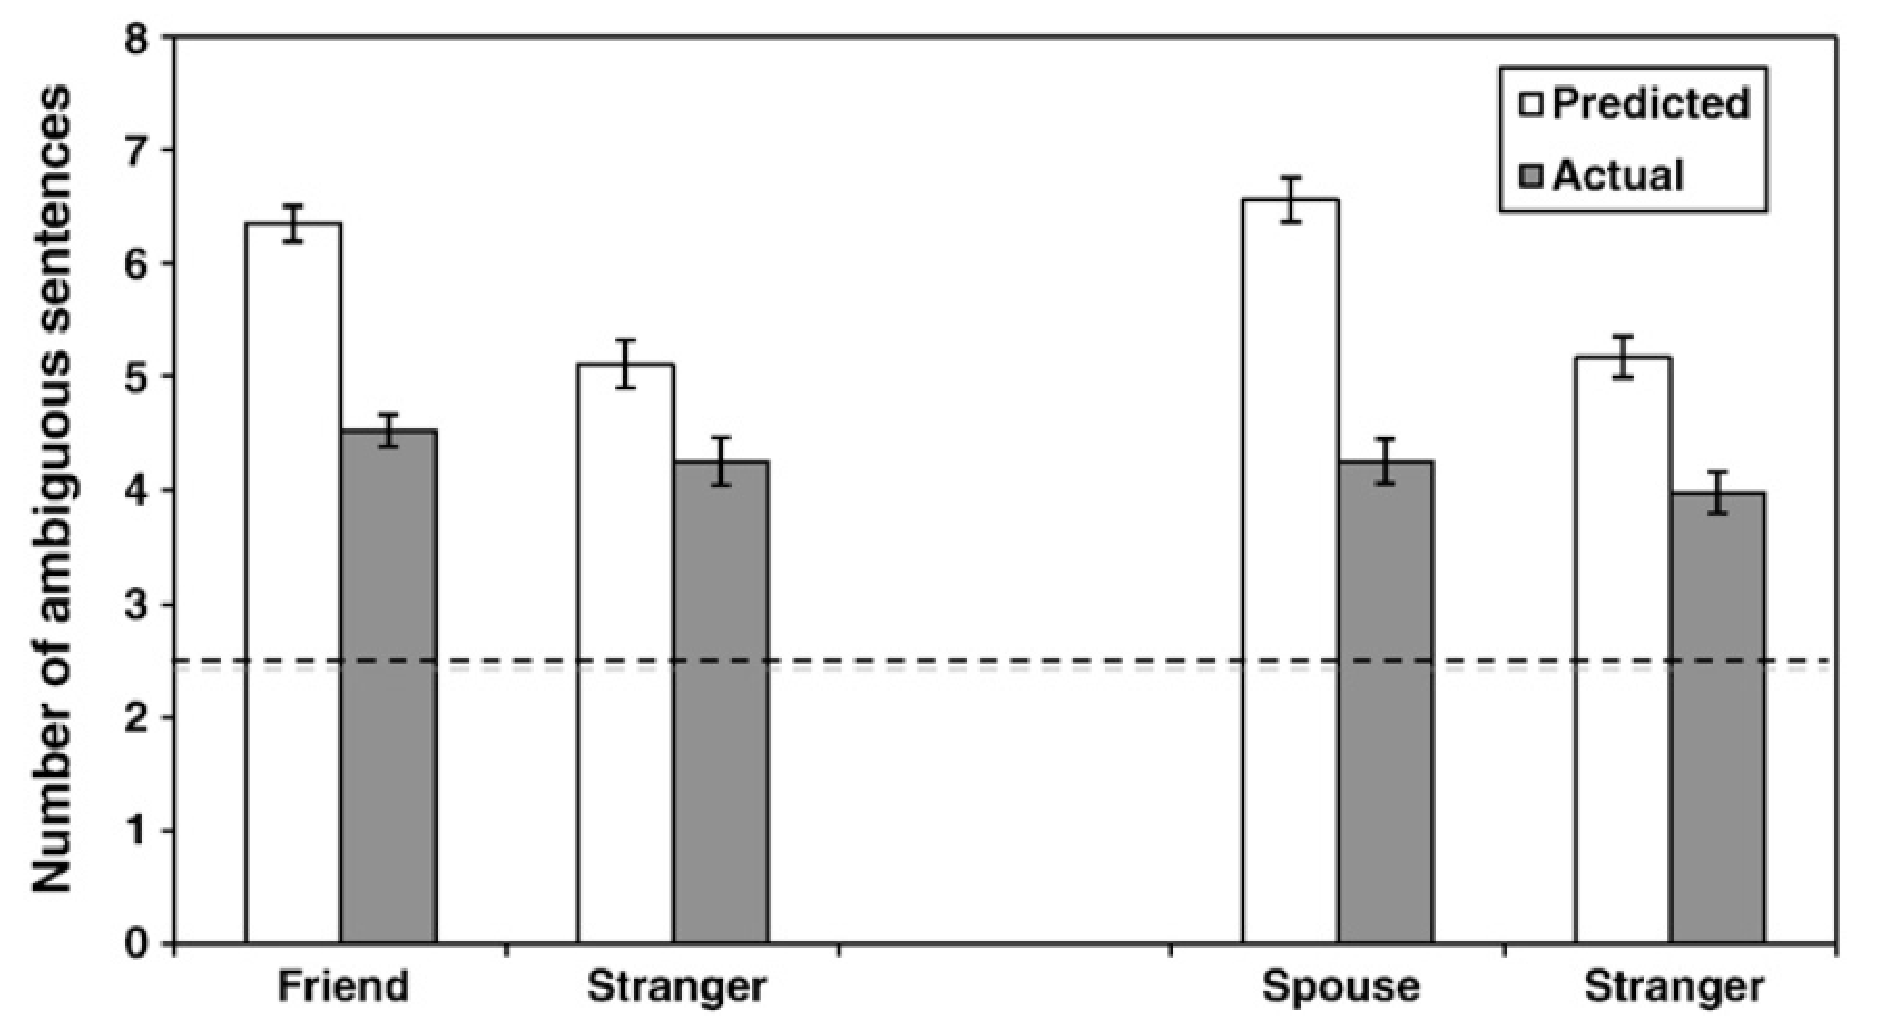
\includegraphics[width=.7\textwidth]{savitsky.pdf}          
%\end{center}
%  \caption{Results from \cite{savitsky-etal:2011}}
%   \label{savitsky}
%\end{figure}
%
%
%\cite{lane-etal2006} offer evidence that is particular germane to the question of discourse status. The experimental design can be seen in Figure \ref{elephants-exp}. Participants were assigned the role of either the speaker or addressee in a communication game. Speakers were instructed to communicate information about a target shape to the addressee. One shape was visible to only the speaker, blocked from the view of the addressee by an occluder. In the target conditions, the item that was visible only to the speaker was the same shape, but varied along some relevant dimension (e.g. size, color). Figure \ref{elephants-results} shows the proportion of trials where speakers used a modifier in referring to the target item. Surprisingly, speakers' privileged information leaks into what is said. In fact, this happens to an even greater extent when speakers were explicitly instructed to conceal information about their privileged information.
%
%
%\begin{figure}
%\begin{center}
%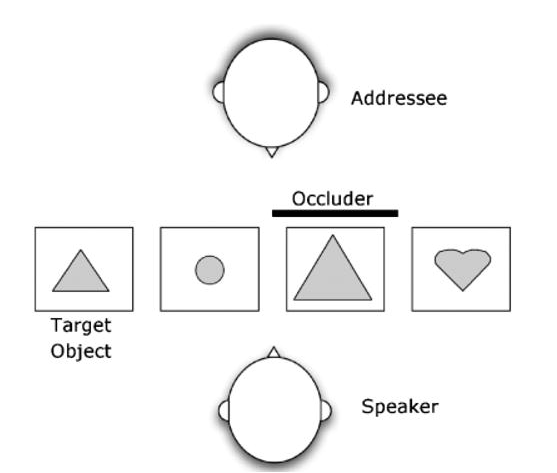
\includegraphics[width=.7\textwidth]{elephants-exp.png}          
%\end{center}
%  \caption{Experimental design of \cite{lane-etal2006}}
%   \label{elephants-exp}
%\end{figure}
%
%
%\begin{figure}
%\begin{center}
%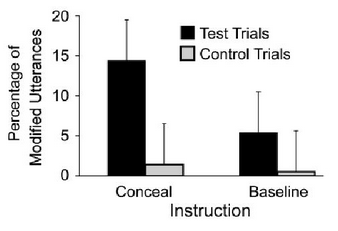
\includegraphics[width=.7\textwidth]{elephant-results.png}          
%\end{center}
%  \caption{Results for \cite{lane-etal2006}}
%   \label{elephants-results}
%\end{figure}
%
%Returning to Jespersen's Cycle, we note that these experimental findings suggest a potential explanation for \emph{why} change takes place. The embracing form is restricted to a particular set of contexts where the proposition being negated is discourse old, or highly inferrable. If speakers tend to overestimate how inferrable the proposition being negated is, if they fail to filter out their own privileged information, then they will tend to use the embracing form in less and less inferrable contexts. The result will be an increase in the frequency of the embracing form over time. \cite{ahern-clark2015} offer a formal model of the dynamics of this process. However, the predictions of the model, like the corpus work by \cite{hansen2009, hansen-visconti2009}, are largely qualitative. That is, they demonstrate that the different forms of negation are sensitive to different constraints at different points in time, and offer an explanation of why those constraints might change over time. However, they offer no 
%quantitative predictions about the shape of the change.
%
%In contrast, \cite{wallage2013} presents a quantitative analysis of the conditioning factors of Jesepersen's Cycle in Middle English, drawing on evidence from the Penn Parsed Corpus of Middle English \citep{ppcme2}. Wallage codes sentences containing sentential negation for the discourse status of the proposition being negated, according to the categories outlined above. From two separate statistical tests on binned data (1150-1250 and 1250-1350), Wallage argues that if we factor out the overall rate of the embracing form, the effect of discourse status is not different across the two time bins. While the argument is interesting and it has great merit in being quantitative, the methodology is not compelling. That is, Wallage uses a form of \href{http://en.wikipedia.org/wiki/Variable_rules_analysis}{VARBRUL} and claims that the coefficients across discourse contexts are similar enough. There are several problems with this approach. First, it doesn't offer any way of quantitatively specifying how similar is 
%similiar \emph{enough}. While regular practice may yield some insight, we want a statistical measure of how similar is similar enough to not reject the hypothesis that the conditioning of discourse status changes. Second, binning the data and not accounting for the potential effects of individual documents may yield misleading results. More appropriate methods, such as generalized linear mixed-effects models (GLMMs) would be more appropriate, and Wallage (p.c.) is moving towards the application of these new statistical techniques.
%
%As it stands though, we don't have a clear answer to whether Jespersen's Cycle is driven by a sensitivity to discourse functional constraints. There are at least two potential explanations that reconcile the findings of \cite{hansen2009, hansen-visconti2009}, the experimental evidence of \cite{lane-etal2006}, the formal model of \cite{ahern-clark2015}, and the null result of \cite{wallage2013}. First, the role of discourse stats in Jespersen's Cycle may differ across languages. That is, the fact that the negation is sensitive to information structure may be particular to Romance languages. In fact, these constraints have only been noted in Romance languages. This could be the result of the constraints only occurring in Romance languages or just a lack of investigation into other languages synchronically and diachronically. The fact that the discourse status conditions in English don't change over time could be explained by this. However, it's striking that, at the beginning of the change, the embracing form 
%in English is largely restricted to Inferrable and Discourse Old contexts. It would be surprising if this were a simple coincidence. Second, absent an explicit model of how and \emph{why} the discourse status constraints might be changing, the methodology employed by Wallage does not tell us much. That is, Wallage implicitly adopts the null hypothesis that the rate of change across discourse contexts is not different and argues that this null hypothesis cannot be rejected. However, it is not entirely clear what the null hypothesis ought to be, or if his method can actually tell us when we can reject it.
%
%While we are still left with a fair amount of uncertainty regarding the actual causes of the cycle, it's clear that answering it will require a quantitative analysis of the conditioning factors of different forms of negation. The downside in this regard is that discourse status is not necessarily a surface property of sentences. That is, we cannot simply take a sentence and read off its relation to the previous discourse. Coding for discourse status requires a careful consideration of the prior context, the potential interpretations of a sentence, and general knowledge about the world.  This task is not straightforward even when analyzing contemporary language equipped with modern intuitions. The difficulty is only exacerbated when we turn to historical corpora. This leads to a reliance on expertise in the historical forms of a language to even perform a qualitative analysis, and a substantial investment of time and expertise to hand-code a large enough set of data to perform a quantitative statistical 
%analysis. Unfortunately, this means that a comprehensive answer to the question of whether discourse constraints are important in Jespersen's Cycle is dependent on having experts in the history of multiple languages where the cycle has occurred invest a significant amount of time towards coding and evaluating the results. This is certainly possible, but also certainly a difficult task.
%
%The goal of this project will be to explore methods for circumventing the need for significant expertise in the history of a language and significant time to understand the role of discourse status in change. In particular, we will be searching for surface properties of sentences that correlated with discourse status. On the assumption that these other surface properties stand in a stable relation to discourse status, we can probabilistically predict the discourse status of particular forms over time. That is, we are trying to infer the surface proxies of discourse status so that we can at least partially automate the process of determining the role of discourse in change. In the next section we describe the methods and data we will use.
%
%

\part{Stability}


% Learning Theory
\chapter{Stability}
\label{Stability}

\setlength{\epigraphwidth}{.9\textwidth}

\epigraph{It may be urged that change in language is due ultimately to the deviations of individuals from the rigid system. But it appears that even here individual variations are ineffective; whole groups of speakers must, for some reason unknown to us, coincide in a deviation, if it is to result in a linguistic change.\\ -- Leonard Bloomfield \citeyearpar[445]{bloomfield1927}}


%All this, de Saussure's la parole, lies beyond the power of our science. We cannot predict whether a certain person will speak at a given moment, or what he will say, or in what words and other linguistic forms he will say it. Our science can deal only with those features of language de Saussure's la langue, which are common to all the speakers of a community,?the phonemes, grammatical categories, lexicon, and so on. 

Distinguishing between the formal and functional Jespersen cycles simplifies the task of explanation. It allows us to disentangle two phenomena that overwhelmingly co-occur, and address them separately. For example, in the previous chapter we showed that the functional cycle in English can be explained in terms of the difficulty speakers have in keeping track of private versus common knowledge.  Crucially, this explanation of the transition from pre-verbal \emph{\textcolor{red}{ne}} to embracing \emph{\textcolor{blue}{ne...not}} rests on the way our pragmatic competence shapes the use and interpretation of linguistic signals over time. 

However, it is important to distinguish between the logical relationship between the two cycles and the explanation of a particular historical change. That is, the functional cycle can occur independently of the formal cycle, so we need an explanation for cases where it does occur independently. But, in the case of English, and many other languages, the functional cycle coincides with the first transition of the formal cycle. There is no guarantee that the model we described to address the functional cycle is the only or even the best explanation of the observed transitions of the formal cycle. That is, in any given case, pragmatic pressures might not explain the first transition of the formal cycle.

Here we consider other potential explanations for both of the transitions of the formal cycle.  In particular, we examine the possible role of acquisition. The facts to be explained are the transition from pre-verbal \emph{\textcolor{red}{ne}} to embracing \emph{\textcolor{blue}{ne...not}} and the transition from embracing \emph{\textcolor{blue}{ne...not}} to post-verbal \emph{\textcolor{green}{not}}. Our goal is to understand whether the process of acquisition offers any insights into why the formal cycle takes place. More broadly, we want to test whether grammatical competence and the process by which it is formed are sufficient to explain the observed changes.

First, we present a model of syntactic acquisition that has several desirable theoretical properties. Second, we determine the dynamics of the model in a population over time. In particular, we show the conditions under which the acquisition dynamics lead to change or stable variation. Third, we outline the syntactic structures at various stages of the formal cycle. These structures allow us to explicitly state the conditions for the acquisition dynamics to lead to either of the transitions of the formal cycle. Finally, we fit the model of the acquisition dynamics to data from the formal cycle in Middle English and discuss the implications of the fitted parameters.  

Acquisition can be taken as a cause of the formal cycle if only if the following qualitative and quantitative criteria are met. First, given the acquisition dynamics and grammatical structures underlying the formal cycle, we should predict the qualitative occurrence of both transitions. Second, if the acquisition dynamics predict the transitions, then the quantitative parameters of the dynamics fit to corpus data should be consistent with our theoretical assumptions. That is, the parameters of the model have some falsifiable empirical content that can be tested using corpus data. If neither of these criteria are met, then acquisition cannot explain the transitions of the formal cycle.

In fact, we show that neither of the transitions of the formal cycle observed in the history of English can be explained by acquisition. First, for the grammatical structures posited to underly the formal cycle the acquisition dynamics predict stability rather than change.  So, the first criterion cannot be met. Second, this also means that the second criterion cannot be met either; given that both transitions do occur, the parameters of the fitted model necessarily differ. In fact, it would seem that the only way acquisition could lead to either of the transitions would be, in Bloomfield's terms, a mass coincidence of deviation from the current system.

The main contributions of this chapter are twofold. First, we offer a general analysis of the acquisition dynamics, which clearly delineates the conditions for stability and change under certain kinds of parametric variation. Second, we make explicit the conditions for acquisition to play a role in either of the transitions of the formal cycle. In particular, one must show not only that acquisition predicts both transitions qualitatively, but that it also matches the quantitative trajectory of the change. It is important to note that these hold for any set of syntactic structures posited to underly the formal cycle. Demonstrating the role of acquisition requires demonstrating how the acquisition dynamics leads from one state to another.


\section{A model of acquisition}

In the most general sense, the process of language acquisition is some mapping from the initial state of the learner and the linguistic evidence provided to the learner to some terminal state, which is taken to be the grammatical competence of the speaker. We begin by introducing a model that can be used to describe this process. We then note some of the properties that make it an appealing model of acquisition.

The \emph{variational learning} model of acquisition \citep{yang2000internal,yang2002} consists of three basic components. First, there is a finite set of grammars that vary in a parametric fashion, in the sense of the  \emph{Principles and Parameters} framework \citep{chomsky1981,chomsky1995,chomsky-lasnik1993}. Second, a learner keeps track of a probability distribution over grammars, which we can think of as the weights of evidence the learner has for the various grammars. Third, a learner updates her distribution over grammars according to a learning scheme as she receives input from the linguistic environment.

To see this in detail, suppose that a learner is presented with sentences from the linguistic environment. The learner selects a grammar $G_i \in G = \{G_1,...,G_n \}$ with probability $p_i$ to analyze a sentence. There are two possible outcomes: either the grammar can analyze the sentence or it cannot. That is, the sentence is grammatical with respect to the selected grammar or it is not. The learner updates her distribution over grammars in the following manner, where $0 < \gamma \ll 1$ is a small learning parameter.


\begin{equation}
 \mbox{If $G_i \rightarrow s$ then }
\left\{
	\begin{array}{ll}
		p_i'  = (1 - \gamma)p_i + \gamma \\
		p_j'  = (1-\gamma)p_j & \mbox{for} j \neq i
	\end{array}
\right.
\end{equation}

\begin{equation}
 \mbox{If $G_i \nrightarrow s$ then }
\left\{
	\begin{array}{ll}
		p_i'  = (1-\gamma ) p_i \\
		p_j'  = (1-\gamma)p_j + \frac{\gamma}{n - 1} & \mbox{for} j \neq i
	\end{array}
\right.
\end{equation}
This is a \emph{linear reward-punishment} scheme \citep{bush-mosteller1955}:\footnote{This learning scheme is similar to the linear reward-inaction scheme that yields the replicator dynamics \citep{borgers-sarin1997}. It differs in that failures are not ignored, but rather punished. One compelling reason for treating learning differently across the domains of meaning and structure is the hypothesis space of each: the grammatical hypothesis space is heavily constrained, whereas the semantic hypothesis space, even under the Fodorian \citeyearpar{fodor1975} conception, is constrained but arguably unbounded. That is, even a finite set of innate concepts can be combined in the appropriate manner without end. Given this quantitative, if not qualitative difference between the domains, it is not clear how a learner would decide what aspects of a given hypothesized meaning to punish (cf. \citealt{quine1960}). But, see \cite{smith-yu2008,medina-etal2011,smith-etal2011, trueswell-etal2013} for experimental evidence, and \cite{yu-smith2007,frank-etal2009,stevens-etal2013} for computational approaches to the problem of learning meaning.} grammars that are compatible with a sentence drawn from the linguistic environment are rewarded, whereas grammars that are not compatible with the sentence are punished. Both of these actions are reflected in the first line of the two possible outcomes. If the grammar can analyze the sentence, then its probability is bumped up by some small amount determined by the learning parameter. If the grammar cannot analyze the sentence, then its probability is knocked down by some small amount determined by the learning parameter. The second conditions allow for the weights over grammars to be redistributed while guaranteeing that all probabilities always sum to one.

Now, the probability that a learner attributes to a grammar changes according to how successful that grammar is in dealing with the linguistic environment. In fact, the long term distribution over grammars can be determined from the probability that a grammar will not be able to analyze a sentence and will thus be penalized. For two grammars, $G_1$ and $G_2$, let the \emph{penalty probabilities} be $c_1$ and $c_2$, respectively. It can be shown that the expected value of the probabilities of the two grammars converge to the following limit values \citep[111]{narendra2012}.
\begin{equation}
\begin{split}
\lim_{t \rightarrow \infty} E[p_1(t)] &= \frac{c_2}{c_1 + c_2 }\\
\lim_{t \rightarrow \infty} E[p_2(t)] &= \frac{c_1}{c_1 + c_2 }
\end{split}
\end{equation}
We should note that this result is about the expected behavior of an individual, rather than the actual behavior of that individual. So, while the expected value of the probabilities converges to these values, the actual probability in the mind of a given learner does not. As we will see below, the actual values in the mind of an individual are close to, but not necessarily equal to these values. This distinction has important implications for the dynamics of acquisition, which we return to in the next section. In particular, it requires us to make certain assumptions about the size of the population.

%Second, the expected value of the probability of a grammar in the limit is directly proportional to the penalty probability of that grammar. Importantly, this means that learners get the appropriate ordering of weights to evidence, which is a property we would arguably expect of any learning model.

%�\footnote{This property holds for an arbitrary number of grammars \citep[117]{narendra2012}.}

So, we know the expected behavior of a learner given the penalty probabilities of the grammars in question. We can determine the penalty probabilities in the following manner. First, suppose that the linguistic environment is composed of the output of two partially incompatible grammars. Let $\alpha_1$ be the proportion of sentences generated at random by the first grammar $G_1$ that the second grammar $G_2$ cannot analyze; likewise let $\alpha_2$ be the proportion of sentences generated at random by the second grammar $G_2$ that the first grammar $G_1$ cannot analyze. Note that while the assumptions underlying them are theoretical both $\alpha_1$ and $\alpha_2$ empirical estimates of both can be calculated from a corpus (e.g. \citealt[94-95]{ingason-etal2013}).  We can represent the relationship between the two grammars visually as in Figure \ref{grammars-evidence} where the overlap of the two grammars indicate the sentences that are jointly analyzable by both grammars.  Second, let the linguistic environment be composed of some distribution over the two grammars, call it $L = p_1G_1 + p_2G_2$.  From this we can calculate the penalty probabilities as $c_1 = p_2\alpha_2$ and $c_2 = p_1\alpha_1$. The likelihood that the first grammar will not be able to analyze a sentence depends on the prevalence of the second grammar in the environment and the likelihood a sentence generated by that second grammar will be incompatible with the first grammar. The same reasoning holds for the second grammar. 

%That is, the likelihood that each of the grammars will not be able to analyze a sentence depends on the independent evidence for the other grammar and its prevalence in the environment.


\begin{figure}
\begin{center}
        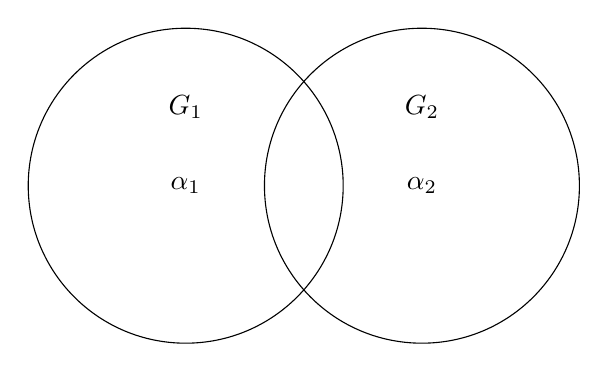
\begin{tikzpicture}
	  \node (A) [draw,circle,minimum size=4cm]  at (0,0) {$\alpha_1$};
	  \node (G1) [above of=A] {$G_1$};
	  \node [draw,circle,minimum size=4cm] (B) at (0:3cm) {$\alpha_2$};
	  \node (G2) [above of=B] {$G_2$};
	\end{tikzpicture}         
    \end{center}
\caption{Two partially incompatible grammars}
\label{grammars-evidence}
\end{figure}

We can get a sense for the learning process by simulating individual trajectories. This can be seen in Figure \ref{lrp-learning} where the horizontal axis represents time as additional sentences drawn from the environment and presented to the learner. The vertical axis represents the weight of $G_2$ in the learner's mind. We can compare the expected motion averaged across several hundred individual trajectories in bold to several individual trajectories. Where the expected motion smoothly approaches the value predicted by the model, shown by the dotted line, individual trajectories continue to move around the value. Again, we return to this important distinction in the next section when we turn to the dynamics of the model.

\begin{figure}
\begin{center}
	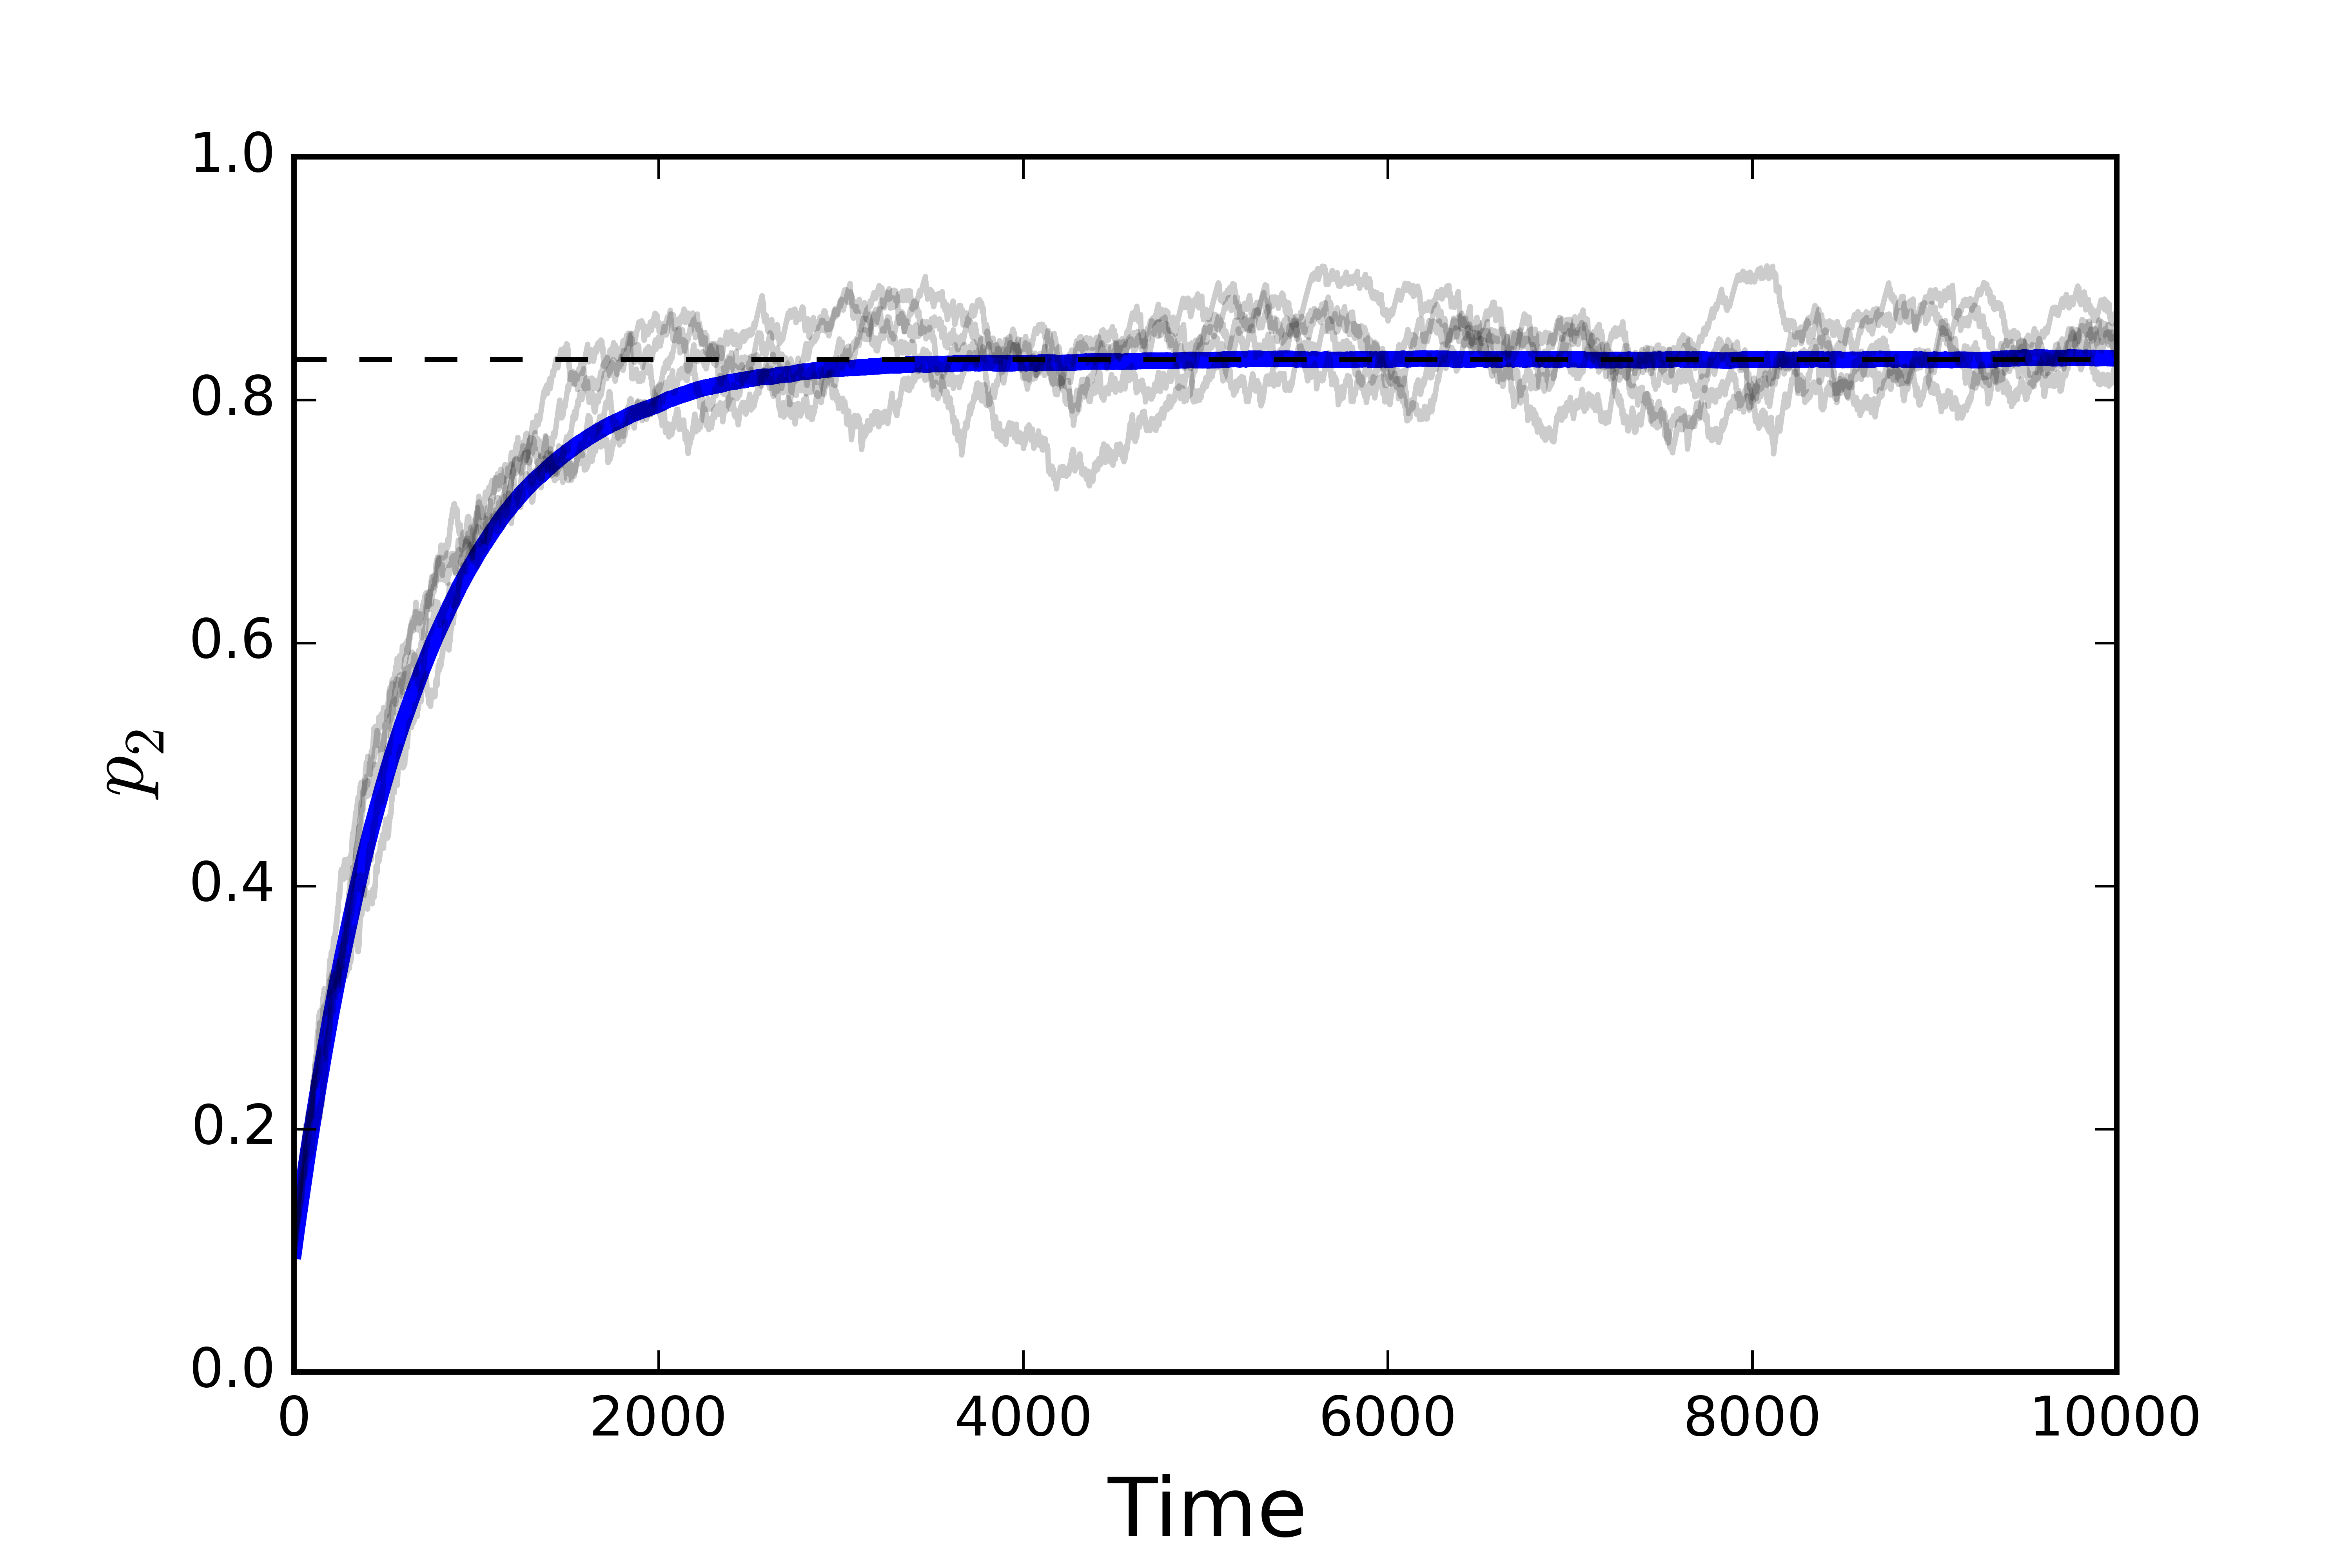
\includegraphics[width=.75\textwidth]{lrp-learning.png}\\
\end{center}
	\caption{Probability of $G_2$ over time for various individual trajectories and expected motion of trajectories, where $L=\frac{1}{2}G_1 + \frac{1}{2}G_2$,  $\alpha_1 = .1, \alpha_2 = .5, \gamma=.1$}
	\label{lrp-learning}
\end{figure}

However, before doing so, there are several important properties that are evident from the simulations presented in Figure \ref{lrp-learning}.  First, this learning model allows for the gradual adjustment of learners to the linguistic environment rather than abrupt changes (cf. \citealt{gibson-wexler1994,hyams-wexler1993}). Second, it allows learners to converge to distributions over grammars, rather than a single grammar \citep{kroch1989}. Third, the expected value of the probability of a grammar is directly proportional to its penalty probability  \citep[117]{narendra2012}, which means that learning is reasonably robust. These properties, along with the overall simplicity of the model make it an appealing starting point for investigating how acquisition might lead to change over time.


\section{The dynamics of acquisition}

We showed the properties of the variational learning model at the level of the individual; we now turn to the dynamics of learning in a population over time. First, we show how the expected change from one point in time to the next gives rise to a particular dynamics under particular assumption. Second, we show that the stable rest points of the dynamics are single grammars, with an important exception. We also show how these dynamics are closely related to the logistic model often taken as a proxy for changes in competing grammars.

Under the variational model, for the case of two grammars, we denote the expected value of the weight accorded to the grammar $G_2$ by a learner to be the following. That is, the average behavior of a learner converges to a probability determined by penalty probabilities and the prevalence of the two grammars in the linguistic environment.

\begin{equation}
p_2' = \frac{p_2 \alpha_2}{p_1 \alpha_1 + p_2 \alpha_2}
\end{equation}
Now, suppose that this distribution in turn serves as the linguistic environment for the next generation of learners. We can determine the expected change in the average weight of $p_2$ from one generation of learners to the next as the following.

\begin{equation}
\dot{p}_2 = p_2' - p_2 = \frac{p_2 \alpha_2}{p_1 \alpha_1 + p_2 \alpha_2} - p_2 = p_2(1-p_2)\frac{\alpha_2 - \alpha_1}{p_1 \alpha_1 + p_2 \alpha_2}
\end{equation}
This \emph{mean dynamics} follows the expected motion of the distribution over grammars in the population. Note that we are talking about the change in the expected behavior in the population. This means that we are modeling a fact about the population as a whole, which ultimately derives from individual learning. However, justifying the mean dynamics requires two important assumptions about the population.

The first assumption that must be made is about the size of the population. As we noted in the previous section, learners converge to the limit values only in expectation. In fact, an individual learner is almost always either slightly above or slightly below this expected value, as can be seen in Figure \ref{lrp-learning}. But, the distribution over these values in a population of learners at a given point in time is roughly normally-distributed around the limit value, as can be seen in Figure \ref{lrp-dist}. In this case, the expected value in the population is close to the limit value. As the population grows, the expected value in the population gets closer and closer to the limit value. In the limit of an infinite population, the linguistic environment for the next generation of learners is the limit value.\footnote{This is often a necessary assumption for studying the mean dynamics of what is undoubtedly a stochastic process. See Chapter 10 of \cite{sandholm2010} for a detailed derivation of the mean dynamics as the limit of a stochastic process in infinite population.    In the next chapter we relax the assumption of an infinite population, allowing for stochasticity in the change in the population over time.}
\begin{figure}
\begin{center}
	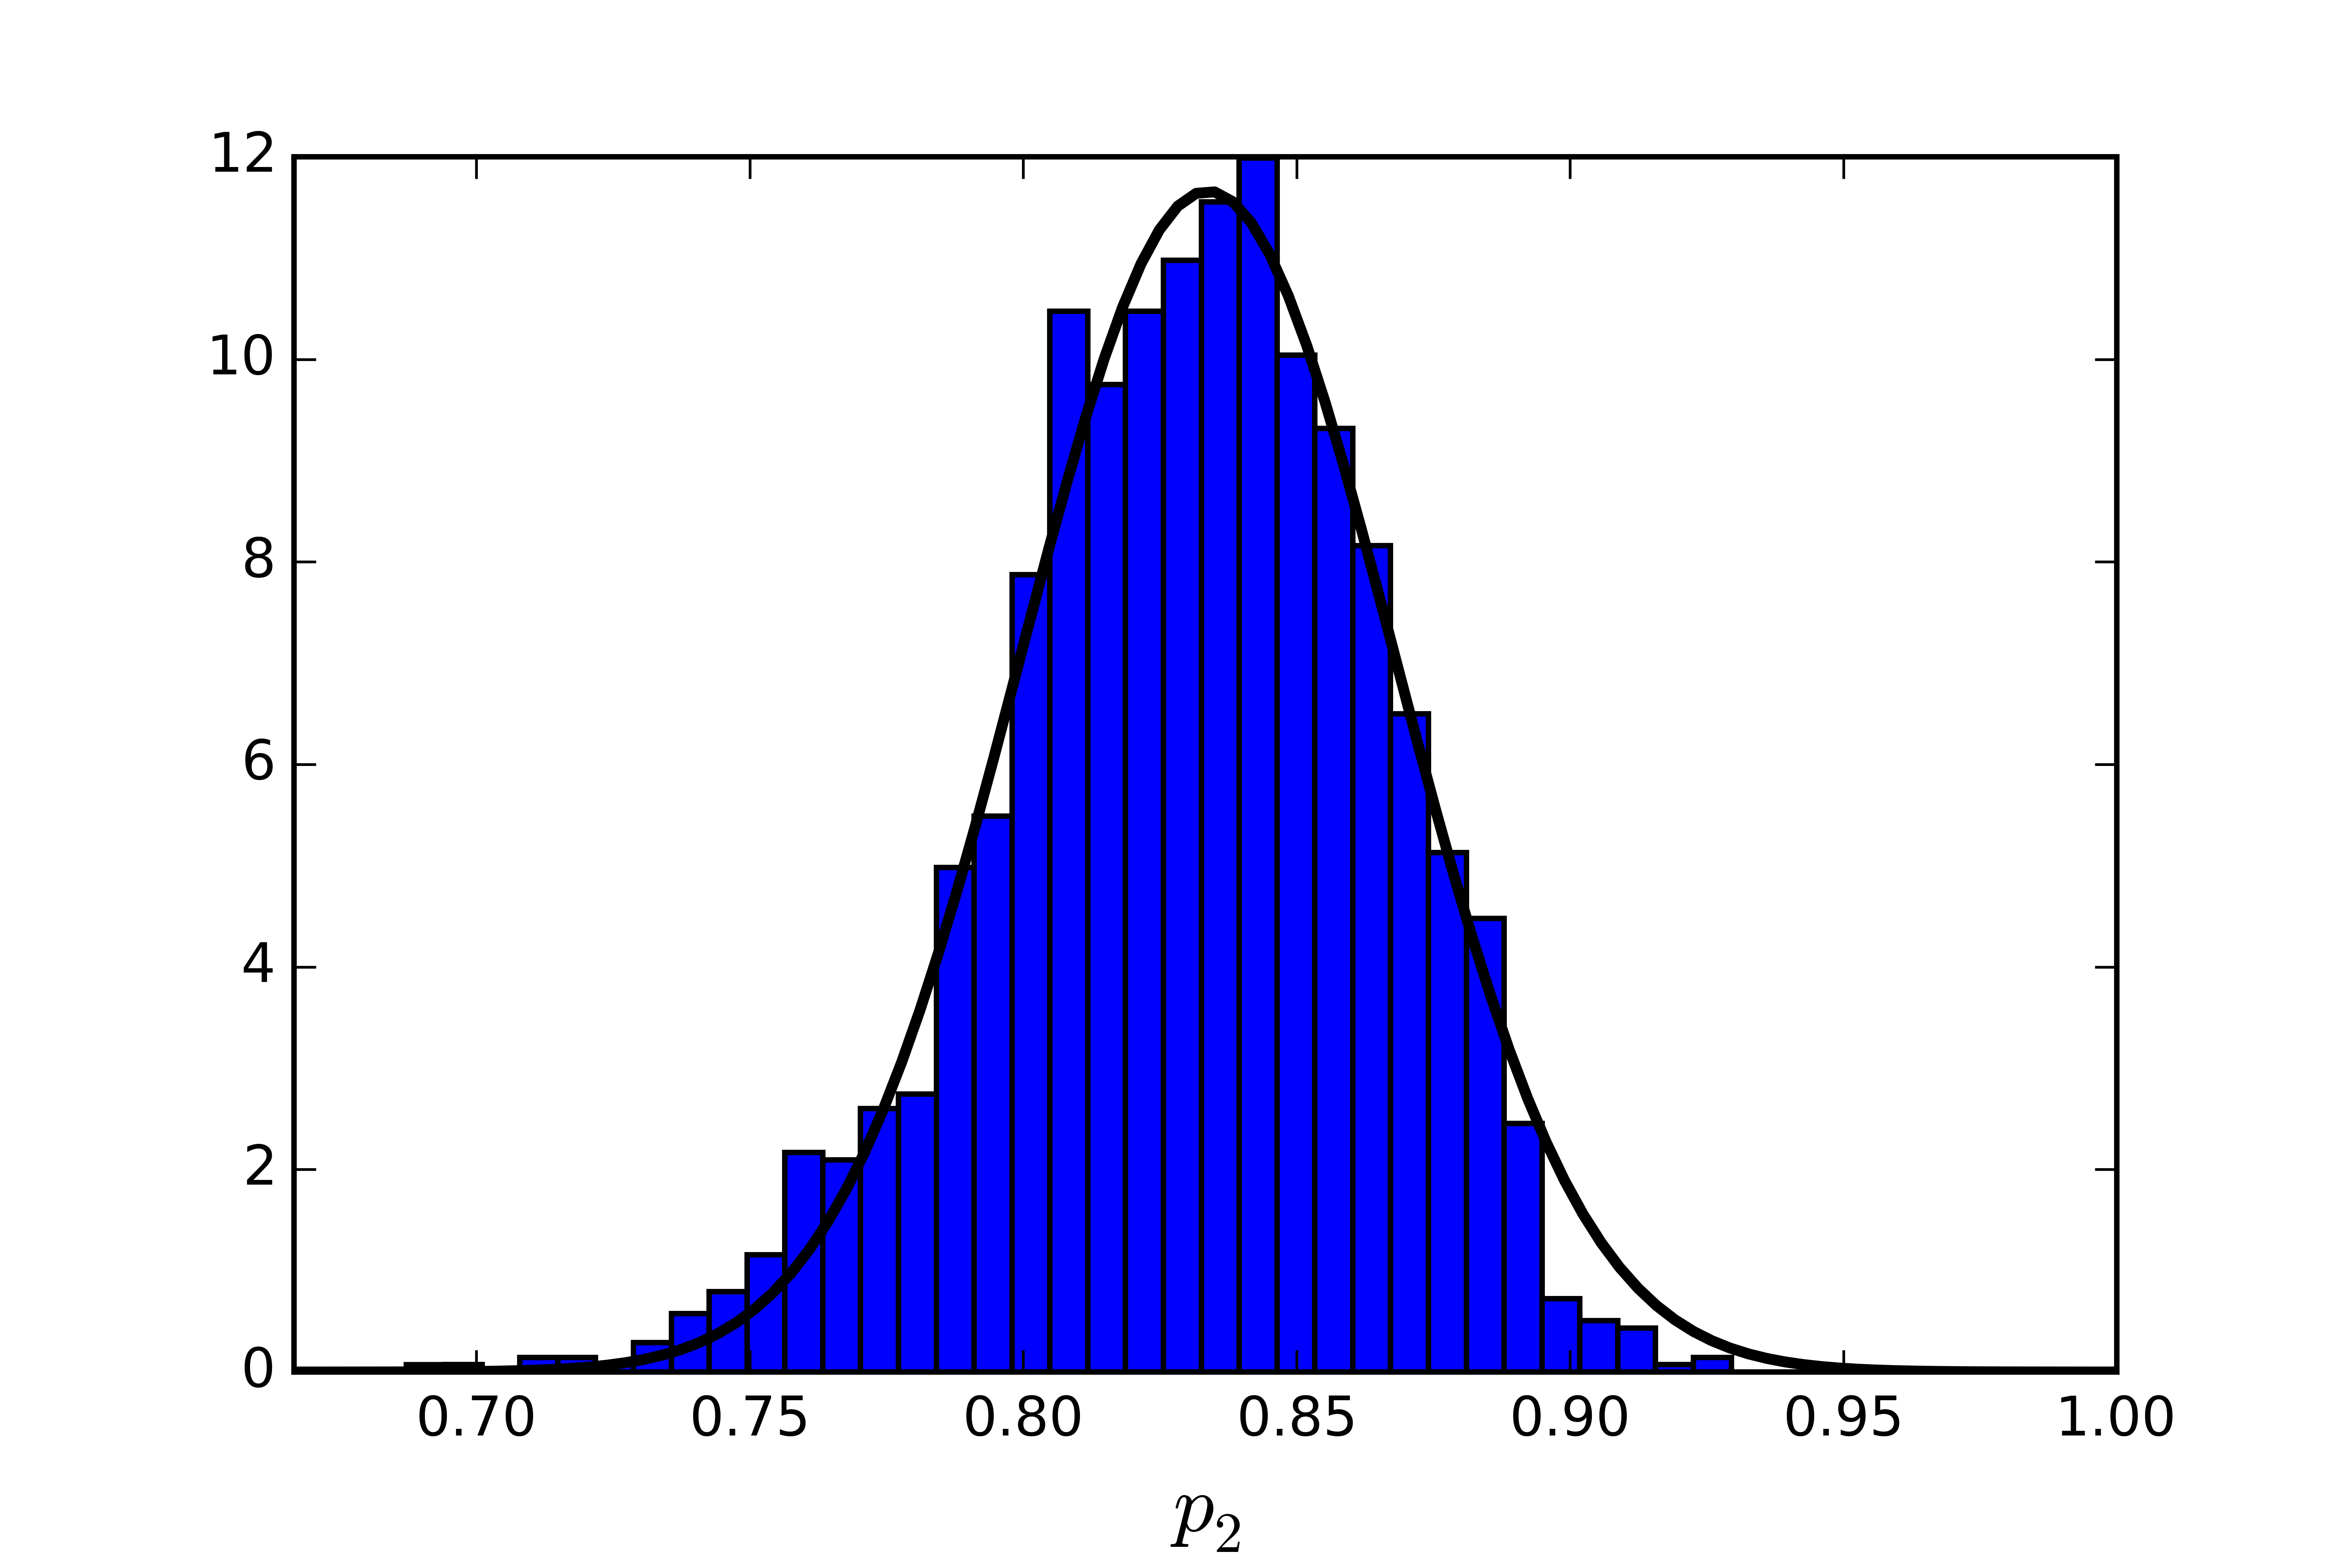
\includegraphics[width=.75\textwidth]{lrp-dist.png}\\
\end{center}
	\caption{Distribution over $p_2$ for population of learners and fitted normal distribution}
	\label{lrp-dist}
\end{figure}

The second assumption that must be made is about the structure of the population. Namely, the continuous-time form of the dynamics requires that we assume that there are continuously overlapping generations of learners that contribute to the linguistic environment.\footnote{A discrete-time dynamics might be more appropriate in allowing for a lag between when learners converge on a grammar and contribute to the linguistic environment, but this  distinction does not affect the subsequent results.} Together these assumptions guarantee that the dynamics track the expected weights over the grammars in the minds of learners over time. Thus, the solutions to this \emph{mean dynamics} is a model of the expected behavior in the population.

For the case of two grammars, we can simplify the dynamics in the following manner. Let $s = \frac{\alpha_2 - \alpha_1}{\alpha_2}$ and $p_2 = p$, then we have the following. In population genetics $s$ is referred to as the \emph{selection coefficient} of $\alpha_1$. For cases where $s > 0$,  $\alpha_2 $ has a selective advantage and $\alpha_1$ is selected against. For $s=0$, $\alpha_1$ and $\alpha_2$ are selectively \emph{neutral}.

\begin{equation}
\dot{p} = p(1-p)\frac{s}{1- s(1-p)}
\end{equation}
We can read the rest points off the resulting acquisition dynamics. There are two important cases that we will consider. First, if there is only a single grammar, then the weight over grammars is stable. That is, if $p=0$ or $p=1$, then the dynamics are, so to speak, at rest.  This makes intuitive sense, a grammar cannot be considered if there is no evidence for it. Second, if there is a perfectly balanced amount of independent evidence for both grammars $s = 0$, then any distribution over grammars is a rest point. This also makes intuitive sense, if the balance of evidence is equally in favor of both grammars, then things should not change. We determine the stability of these sets of rest points in turn.

For the first set of rest points, we can evaluate the stability of a single grammar as a function of the selection coefficient, which captures the ratio of independent evidence in favor of one or the other grammar. To do so we evaluate the derivative of the dynamics at the two rest points constituted by a single grammar. If the derivative evaluated at the rest point is negative, then the rest point is \emph{asymptotically stable}. That is, the dynamics will carry the population to the rest point. If the derivative evaluated at the rest point is positive, then the rest point is \emph{unstable}. That is, the dynamics will carry the population away from the rest point. We can express these conditions as a function of the selection coefficient, $s$. 

\begin{equation}
\frac{\partial \dot{p}}{\partial p} \big|_{p=0} = \frac{s}{1-s}
\end{equation}

\begin{equation}
\frac{\partial \dot{p}}{\partial p} \big|_{p=1} = -s
\end{equation}
Note that for $s \neq 0$, only one of these rest points can be asymptotically stable. The rest point $p=0$ is asymptotically stable if and only if $s < 0$. That is, the population will eventually use grammar $G_1$ exclusively if only if there is more evidence for it than there is $G_2$. The rest point $p=1$ is stable if and only if $s > 0$. That is, the population will eventually use grammar $G_2$ exclusively if and only if there is more evidence in favor of it. 

In fact, these conditions for the stability of both rest points are rather general. If we assume that the selection coefficient is not zero, then there are no other rest points. So, these conditions amount to conditions for \emph{global asymptotic stability}. Importantly, this means that no matter the initial distribution over grammars, if $s > 0$ then grammar $G_2$ will take over in the population. Thus, the acquisition dynamics are a kind of frequency-independent selection. We can get a sense for this fact by visualizing trajectories from the same low starting state of $p$ for various values of $s$ as in Figure \ref{lrp-gain}. No matter how small the initial proportion or slim the margin of evidence, it is guaranteed to eventually go to completion. 

%Under these dynamics, acquisition is a particularly robust process over time.

%\footnote{\citet[239]{yang2000internal} refers to this as the \emph{fundamental theorem of language change}.}

\begin{figure}
\begin{center}
 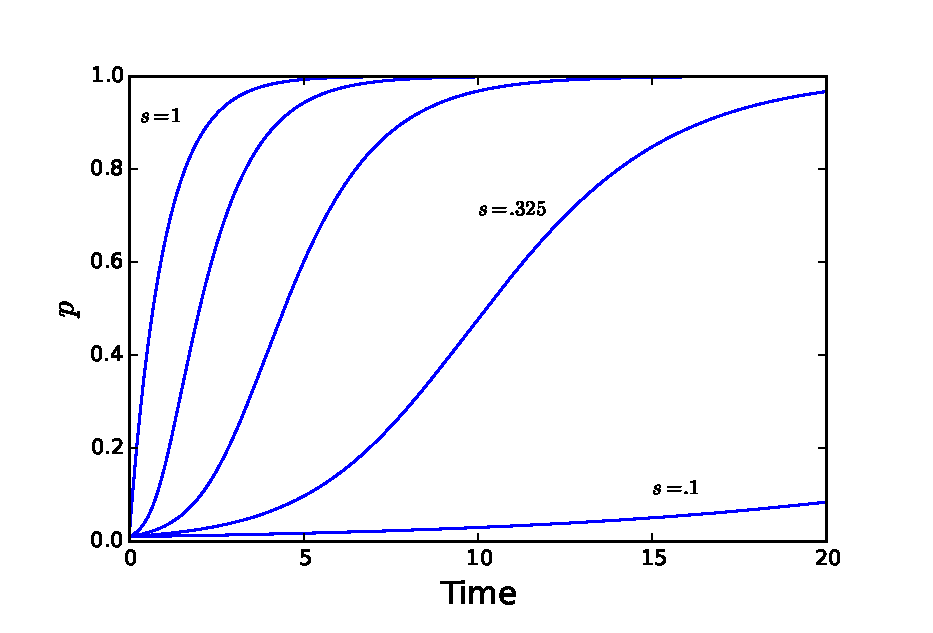
\includegraphics[width=.75\textwidth]{lrp-gain.eps}\\
\end{center}
	\caption{Proportion of $G_2$ over time for various ratios of evidence $s > 0$}
	\label{lrp-gain}
\end{figure}


Interestingly, the acquisition dynamics in these cases are closely related to the logistic models originally posited by \cite{altmann-etal1983} and \cite{kroch1989} to underly competing grammars. While there was no specific learning mechanism underlying the logistic model, it has both connections with the notion of biological competition as well as a straightforward application in terms of logistic regression (cf. \citealt[4]{kroch1989}). However, it is obvious that the variational model provides some justification for this conception when we compare the dynamics of logistic growth with the acquisition dynamics, where $s$ is taken as the growth rate in the logistic model.

\begin{equation}
	\dot{p} = p(1-p)s
\end{equation}
In fact, the only difference is that the acquisition dynamics exhibits a varying growth rate as a function of the distribution over grammars in the population. We show the solution for the acquisition dynamics and the logistic model from the same starting point with the same growth rate in Figure \ref{lrp-log}. The solution to the acquisition dynamics predicts a faster initial rate of growth, but slows down to the same rate as the logistic as $p \approx 1$.

\begin{figure}
\begin{center}
 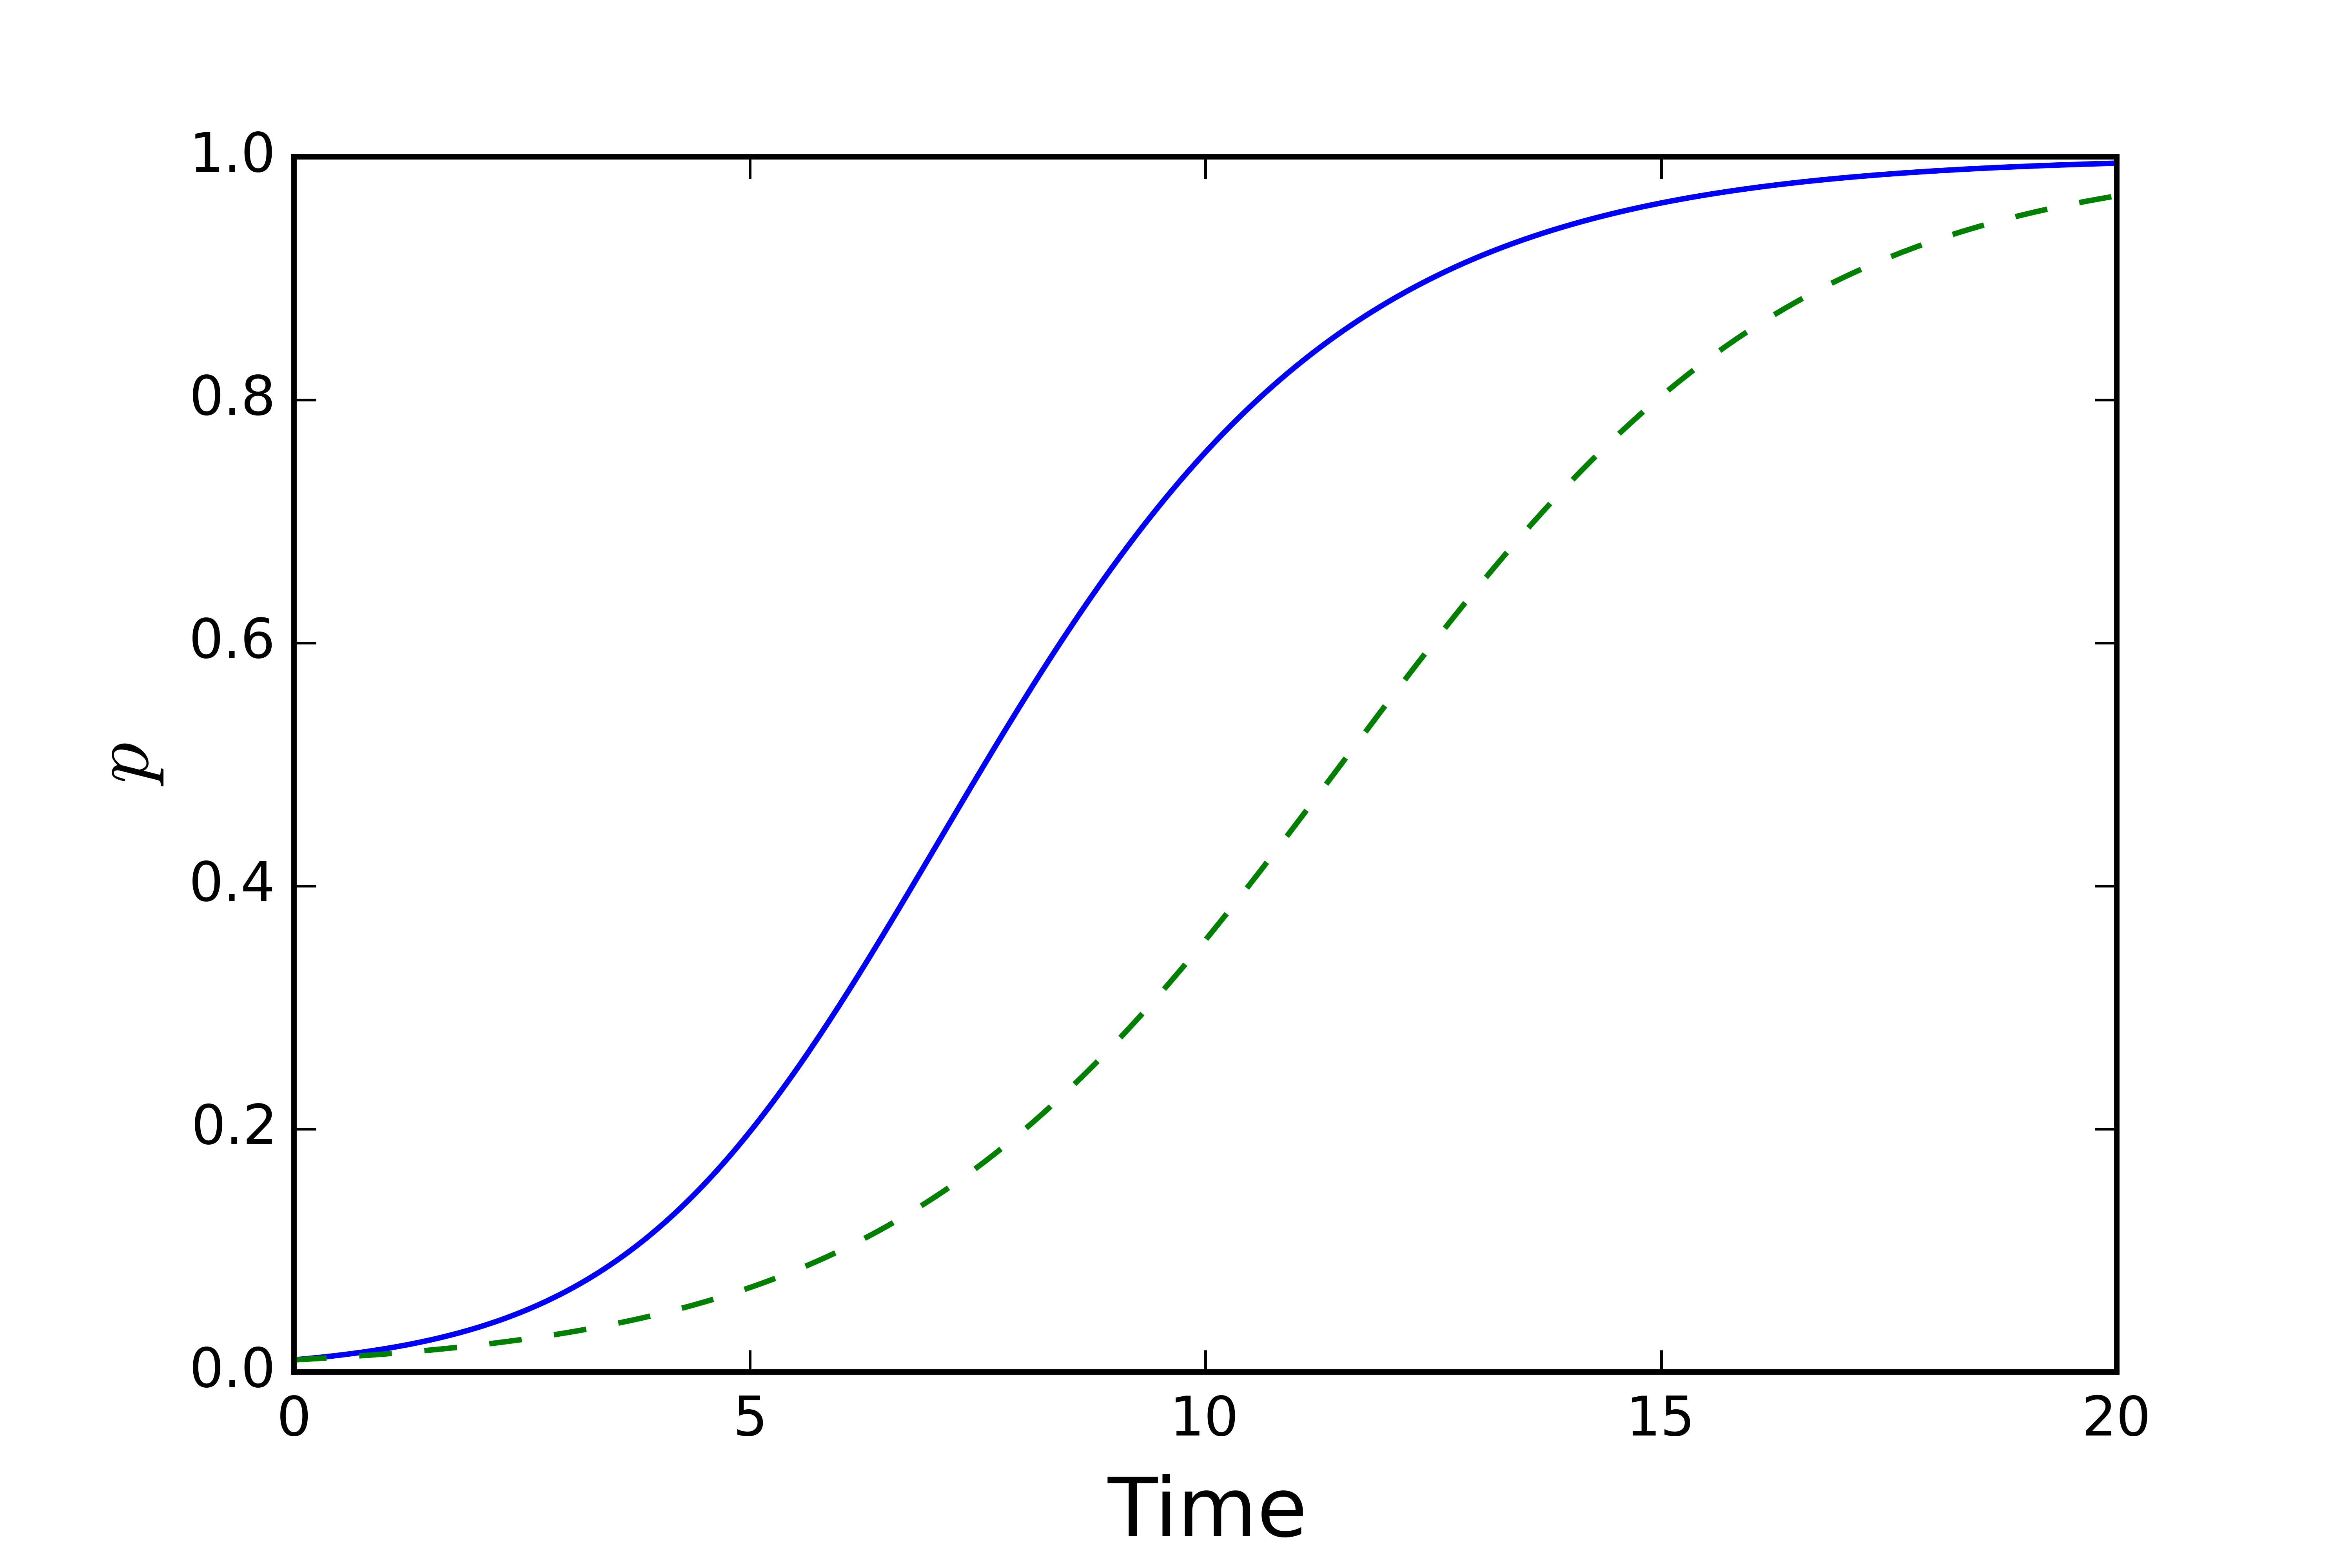
\includegraphics[width=.75\textwidth]{lrp-log.png}\\
\end{center}
	\caption{Solution to acquisition dynamics and logistic model (dashed) from same starting point with $s=.4$}
	\label{lrp-log}
\end{figure}


In many cases the predictions of the two underlying models may not be distinguishable. But, it is certainly possible that we might detect quantitative evidence for the acquisition dynamics. For example for selection coefficients $s \approx 1$ the acquisition dynamics are asymmetric, unlike the logistic, which is perfectly symmetric. This can be seen in the first few solutions in Figure \ref{lrp-gain}. In the context of regression this could potentially lead to quantitative patterns such as heteroscedastic residuals. For example, if we take the acquisition dynamics as a generative model, then fit of the logistic model may systematically under or overestimate the rate of change at different points. We leave investigating this possibility for future research. 

For the second set of rest points, where both grammars have equal independent evidence $s=0$, all distributions over grammars are rest points. All states are \emph{weakly} or \emph{lyupanov stable} in the sense that though the dynamics do not carry the population to a state, the also do not carry the population away from it. Now, we might wonder whether these seemingly knife-edge cases are likely if even possible. However, these cases have a natural interpretation and one that will be particular relevant to the formal cycle. That is, they describe cases where the difference between two grammars hinges on the expression of a single syntactic position. If two grammars correspond to two ways of expressing that position, then the output of each will be incompatible with the other. That is, they will be totally mutually incompatible grammars, rather than only partially incompatible grammars. This can be visualized as in Figure \ref{grammars-incompatible}, which stands in contrast with Figure \ref{grammars-evidence}. In other words, where two grammars vary parametrically at the appropriate level, the dynamics predict a kind of weak stability.

\begin{figure}
\begin{center}
        \begin{tikzpicture}
	  \node (A) [draw,circle,minimum size=4cm]  at (0,0) {$\alpha_1$};
	  \node (G1) [above of=A] {$G_1$};
	  \node [draw,circle,minimum size=4cm] (B) at (0:5cm) {$\alpha_2$};
	  \node (G2) [above of=B] {$G_2$};
	\end{tikzpicture}         
    \end{center}
\caption{Two totally incompatible grammars}
\label{grammars-incompatible}
\end{figure}


So, we determined the acquisition dynamics resulting from the variational model and showed how it exhibits a kind of frequency-independent selection. That is, in most cases only a single grammar is stable. We showed how the resulting dynamics resembles the logistic model of growth. We also noted a crucial exception to this rather robust behavior that leads to a weak kind of stability.  With this in mind, we now turn to an analysis of the syntactic structures underlying the formal cycle.

\section{The syntactic structures of the formal cycle}

There are a range of ways of analyzing the syntactic structures underlying the formal cycle.\footnote{For example, different analyses have suggested varying levels of detail in the number and realization of stages, ranging from three stages  \citep{burridge1983,bernini-ramat1996,haspelmath1997,frisch1997,zanuttini1997,horn:1989,hoeksma1997,horn2001,roberts-roussou2003,vanderAuwera-neuckermans2004,mazzon2004,willis2005,lucas2007,jager2008,wallage2008}, to four stages \citep{dahl:1979,schwegler1988,schwegler1990,schwenter2005,schwenter2006}, up to five stages \citep{honda2000,beukema1999,vanderAuwera-neuckermans2004,zeijlstra2004}.} Here we focus on the analysis presented in \cite{frisch1997}, which treats the formal cycle as the result of two independent morphological changes. First, we present the theoretical details of the analysis. We then note corpus evidence in favor of this treatment.

% Finally, we explicitly state the grammars posited to underly the formal cycle.


\cite{frisch1997} takes Pollock's \citeyearpar{pollock1989} analysis of  negation as a starting point, assuming that negation constitutes its own phrase, with a fully projected structure like that in Figure \ref{negp}: Neg$^0$ is the head of the phrase, Spec is its specifier, and XP is a sister phrase such as a verb phrase.  In particular, Frisch assumes that this underlying structure is always present  \citep{haegeman1995}. The formal cycle simply consists in changes to how the positions in this underlying structure are expressed.\footnote{This is a more localized version of the  \emph{cartographic approach} advocated by \cite{rizzi1997}, which posits a universal syntactic structure. The locus of variation between languages under this conception is how that universal structure is expressed.}


\begin{figure}
        \Tree [.NegP [. Spec ]
        [.Neg$'$ Neg$^0$
        XP ] ]

\caption{The structure of the Negative Phrase} 
\label{negp}
\end{figure}

%However, he treats the embracing form as epiphenomenal, arising from two independent morphological changes in a fixed underlying structure. The assumption of a fixed structure can be stated as in Haegeman's \citeyearpar{haegeman1995} \emph{Neg-criterion} on negative phrases.
%
%\begin{definition}
%The Neg-criterion
%\begin{enumerate}
%	\item Each Neg $X^0$ must be in a spec-head relationship with a Neg operator.
%	\item Each Neg operator must be in a spec-head relationship with a Neg $X^0$.
%	\item Neg-operator: a NEG phrase in a scope position
%	\item Scope position: a left-peripheral A -position (i.e. XP-adjoined or Spec).
%\end{enumerate}
%\end{definition}

%This criterion simply requires that the negative phrase always have the full structure as in Figure \ref{negp}, including a head and a specifier. The strongest form of this assumption posits a universal syntactic structure, where the locus of variation between languages lies in how this universal structure is expressed (cf. the \emph{cartographic} approach advocated by \citealt{rizzi1997}, \emph{inter alia}).

At the first stage of the formal cycle the negative head is expressed as \emph{ne} whereas the specifier is a phonologically null operator $\varnothing$. The syntactic structure according to this morphological analysis can be seen in Figure \ref{stage1morphology}. Sentential structure at stage one of the formal cycle in Old English is illustrated in Figure \ref{sentence1morphology}, where a strikethrough indicates successively upwards head movement. The result is purely pre-verbal negation.

%$_{[+\text{NEG}]}$
\begin{figure}
        \Tree [.NegP [.XP $\varnothing$ ]
        [.Neg$'$ [.Neg \emph{ne}
        ] [.VP \edge[roof]; {...} ] ] ]

\caption{Stage one of the formal cycle according to morphological analysis}
\label{stage1morphology}        
\end{figure}


\begin{figure}
        \Tree [.TP [.DP ic ] [.T$'$ [.V+Neg+T {ne secge} ] [.NegP $\varnothing$
        [.Neg$'$ [.\sout{V+Neg}
        ] [.VP \sout{V} ... ] ] ] ] ]

\caption{Sentential structure at stage one of the formal cycle according to morphological analysis}
\label{sentence1morphology}
\end{figure}

The transition to the second stage in the formal cycle stems from a change in the realization of the specifier of the negative phrase. Namely, the specifier is no longer expressed by a null operator, but instead by \emph{not}, as can be seen in Figure \ref{stage2morphology}. Sentential structure at the second stage of the formal cycle in Middle English is illustrated in Figure \ref{sentence2morphology}, which results in pre- and post-verbal negative elements.


\begin{figure}
        \Tree [.NegP [.XP \emph{not} ]
        [.Neg$'$ [.Neg \emph{ne}
        ] [.VP \edge[roof]; {...} ] ] ]

\caption{Stage two of the formal cycle according to morphological analysis}
\label{stage2morphology}        
\end{figure}


\begin{figure}
        \Tree [.TP [.DP I ] [.T$'$ [.V+Neg+T {ne seye} ] [.NegP \emph{not}
        [.Neg$'$ [.\sout{V+Neg}
        ] [.VP \sout{V} ... ] ] ] ] ]

\caption{Sentential structure at stage two of the formal cycle according to morphological analysis}
\label{sentence2morphology}
\end{figure}

%At this point in the formal cycle we might wonder whether the introduction of two negative elements is problematic. That is, if each element contributes semantic negation in its own right, then the two might cancel each other out. In classical terms, a doubly negated proposition is logically equivalent to the bare proposition.  To circumvent this problem \cite{frisch1997} argues for the \emph{Economy of Projection} principle posited independently by \cite{speas1994}.

%\footnote{Of course, this equivalence ceases to hold in intuitionistic logic, which abandons the elimination of double negation $\neg \neg p \leftrightarrow p$ and the law of the excluded middle $p \vee \neg p$ in favor of a proof-theoretic approach.}

%\begin{definition}
%Economy of Projection principle
%\begin{enumerate}
%	\item Project a phrase XP only if XP has content
%\end{enumerate}
%\end{definition}

%This principle simply states that we can only posit syntactic structure where we have some evidence for it. In this case, the negative phrase is licensed if it contains material in either the head or the specifier. In other words, neither element is necessary for the phrase to occur, so neither can be responsible for the contribution of negative meaning by itself. Rather, it is the negative phrase as a whole that contributes semantic content of negation to the sentence. This can be seen in Figures \ref{stage1morphology} and \ref{stage2morphology} where it is the entire negative phrase that carries the $[+\text{NEG}]$ feature of semantic negation.

The transition from the second stage to the third and final stage of the formal cycle is simply a a matter of whether the negative head is expressed via lexical content or by some null head $\varnothing$. The structure of the negative phrase at the third stage is shown in Figure \ref{stage3morphology}, and sentential structure at this final stage in Late Middle English is shown in Figure \ref{sentence3morphology}. 

%Subsequent stages of negation can be derived by considering the loss of verb raising and the rise of \emph{do}-support.

\begin{figure}
        \Tree [.NegP [.XP \emph{not} ]
        [.Neg$'$ [.Neg $\varnothing$ ]
        [.VP \edge[roof]; {...} ] ] ] 

\caption{Stage three of the formal cycle according to morphological analysis}
\label{stage3morphology}
\end{figure}

\begin{figure}
        \Tree [.TP [.DP I ] [.T$'$ [.V+Neg+T {say} ] [.NegP \emph{not}
        [.Neg$'$ [.\sout{V+Neg}
        ] [.VP \sout{V} ... ] ] ] ] ]

\caption{Sentential structure at stage three of the formal cycle according to morphological analysis}
\label{sentence3morphology}
\end{figure}

Similar morphological approaches to the formal cycle are adopted by \cite{roberts-roussou2003} and \cite{zeijlstra2004}. The shared aspect of these morphological analyses is the assumption that the underlying syntactic structure remains stable, but the realizations of particular positions within that structure changes. Importantly, since this is the only locus of change, the transitions that constitute the cycle are independent of each other. That is, the fact that both \emph{ne} and \emph{not} show up in the embracing \emph{\textcolor{blue}{ne...not}} form is simply the coincidental product of two forms waxing and waning at the same time.

\cite{frisch1997} tests this theoretical prediction using the trajectory of negation in Middle English in the Helsinki corpus of Middle English. He notes that if the two transitions are independent of each other, then the co-occurrence of \emph{ne} and \emph{not} in the negative phrase should be the product of the probabilities of each occurring. 

\begin{equation}
	P(\emph{\textcolor{blue}{ne...not}}) = P(\emph{ne})P(\emph{not})
\end{equation}
That is, the probability of \emph{\textcolor{blue}{ne...not}} is the probability of two independent events \emph{ne} and \emph{not}. This is in fact what Frisch finds.\footnote{Calculating these probabilities requires some adjustment for things like instances of adverbial \emph{not} among others. See \citet[32-47]{frisch1997} for the details.} So the formal cycle can be conceived of as two changes in the expression of positions within an underlying structure. In what follows, we will assume that grammatical knowledge is represented as in Figures \ref{stage1morphology}, \ref{stage2morphology}, and \ref{stage3morphology}. That is, under the assumption of a constant underlying structure, a grammar is characterized by the mapping from the syntactic positions in the negative phrase to lexical items. With these definitions in place, we turn to the actual trajectories of the transitions of the formal cycle in English.


%Frisch estimates the probabilities required to test this prediction in the following manner. First, he estimates the total tokens of \emph{ne} by simply counting the appearances of \emph{ne}. Second, the number of relevant \emph{not} tokens has to be adjusted to exclude adverbial tokens of \emph{not}, which are not part of the negative phrase. Frisch uses the distribution of the adverbial \emph{never} pre- and post-verbally to estimate the proportion of adverbil \emph{not}. Namely, if adverbial \emph{not} is distributed in similar proportions pre- and post-verbally, then the total number of adverbial \emph{not} tokens can be estimated from the total number of pre-verbal tokens. With this adjustment, the probability of both \emph{ne} and \emph{not} can be calculated and compared to their joint probability. Treating the embracing form in this manner yields a good fit to the data.

%\footnote{See \cite[52]{frisch1997} Table 13 for details of the $\chi ^2$ test results. See Tables 9, 10, and 11 for the construction of Table 13.}

%If the appearance of \emph{ne} and \emph{not} together as \emph{\textcolor{blue}{ne...not}} is simply coincidental, then how are we to characterize the grammatical knowledge underlying the different stages of the formal cycle? I


%So, the grammar at the first stage of the formal cycle maps the head of the negative phrase to \emph{ne} and the specifier to a null operator $\varnothing$, the grammar at the second stage of the formal cycle maps the head to \emph{ne} and the specifier to \emph{not}, and the grammar at the third stage of the formal cycle maps the head to a null element $\varnothing$ and the specifier to \emph{not}.

%\begin{equation}
% \mbox{$G_1 : $}
%\left\{
%	\begin{array}{ll}
%		Neg^0 \rightarrow ne\\
%		Spec \rightarrow \varnothing
%	\end{array}
%\right.
%\end{equation}
%
%\begin{equation}
% \mbox{$G_2 : $}
%\left\{
%	\begin{array}{ll}
%		Neg^0 \rightarrow ne\\
%		Spec \rightarrow not
%	\end{array}
%\right.
%\end{equation}
%
%\begin{equation}
% \mbox{$G_3 : $}
%\left\{
%	\begin{array}{ll}
%		Neg^0 \rightarrow \varnothing \\
%		Spec \rightarrow not
%	\end{array}
%\right.
%\end{equation}
%With these definitions in place, we turn to the actual trajectories of the transitions of the formal cycle in English.

%\footnote{\citet[56]{frisch1997} explicitly assumes that the formal cycle is simply a transition from one method of licensing the negative phrase to another, and ``does not necessitate invoking two underlying grammars (\emph{I-languages} in the sense of \cite{chomsky1986}), as the old and new systems do not vary on a particular parameter." This is, perhaps, a strange characterization insofar as the first and last stages do indeed vary parametrically with regard to whether the head and specifier of the negative phrase are expressed by non-null elements.}


%At the heart of this question is the amount of evidence that a given element expresses negation. At the beginning of the change clearly only the preverbal negator does so. The postverbal reinforcer only emphasizes this negation. Eventually though, the evidence weighs in favor of the postverbal negator alone being the expression of negation. \cite{wallage2008} characterizes this transition in morphosyntactic terms as the loss of a [+NEG] feature on the preverbal negator, along with the concomitant introduction of a [+NEG] feature on the postverbal negator. This then allows for the loss of the preverbal negator given that the negative feature can be found elsewhere in the sentence.


%We can formulate the effect of various amounts of evidence in terms of Yang's \citeyearpar{yang2002} variational model. First, let there be two grammars, $G_{ne}$ and $G_{not}$, that represent the location of the abstract feature at \emph{ne} and \emph{not} respectively. We can represent the relation between the two grammars schematically as in Figure \ref{grammars}. In this case, $\alpha$ indicates the proportion of the linguistic environment that is only compatible with $G_{ne}$, and $\beta$ indicates the portion of the linguistic environment that is only compatible with $G_{not}$. The proportion of the two grammars in the population is governed by the following learning rule, where $p_0$ and $p_t$ represent the proportion of $G_{ne}$ in the population after $0$ and $t$ generations, and $q_0$ and $q_t$ represent the proportion of $G_{not}$ after $0$ and $t$ generations.


\section{Modeling the formal cycle}

%Now a problem of parameter interference immediately arises. Under the parametric representation of grammars, grammar selection is based on independent parameters. By contrast, fitness measure and thus the outcome of learning�reward or punish- ment�is defined on whole grammars.

Now that we have stated the grammars underlying the stages of the formal cycle we can turn to modeling the transitions of the formal cycle. First, we note that given the structure of the grammars posited to underly the formal cycle, we can treat each of the transitions separately. Second, we note that given the composition of the grammars we should expected stability under the acquisition dynamics. Finally, we fit the acquisition model for the two transitions of the formal cycle and note that the parameters are indeed not what the acquisitions dynamics predict. However, we note what a successful explanation of the formal cycle would have to do.

The grammars underlying the formal cycle differ only in the expression of two syntactic positions. This has two important implications. First, if the two changes in how these positions are expressed are independent of each other, then we can treat them as such. That is, we can treat the two transitions of the formal cycle as independent events of competition between two grammars for expressing those positions. In what follows we take this approach, treating both the first and second transitions as cases of the acquisition dynamics with two grammars. Second, if the grammars involved in each transition differ only in the expression of one position, then they are totally mutually incompatible $s=0$. This means that the acquisition dynamics predict stability in the case of both transitions, but this is certainly not what we observe. In fact, this alone suffices as a demonstration that acquisition as we have modeled it here cannot account for either of the transitions of the formal cycle.  That is, given the description of the grammars underlying the stages of the formal cycle, acquisition cannot cause the transitions between them. This means that the qualitative criterion for acquisition serving as a cause of the formal cycle is not met.

However, it is useful to note what would have to be the case for acquisition to explain the empirical trajectories of the two transitions. That is, if we fit the acquisition dynamics to data, the fitted parameters tell us what we would need to find in order to take acquisition as the cause of the formal cycle. We fit the acquisition dynamics to the trajectory of the first transition modeled as the competition of two grammars for the specifier of the negative phrase. In this case we take $G_1$ as $G_\varnothing$ and $G_2$ as $G_{not}$ to be grammars that determine how the specifier of the negative phrase is expressed.  We take instances of \emph{\textcolor{red}{ne}} to be compatible with $G_\varnothing$ and instances of \emph{\textcolor{blue}{ne...not}} and  \emph{\textcolor{green}{not}} to be compatible with $G_{not}$. The parameters to fit are the initial state of the second grammar in the population and the selection coefficient  $s$ that captures the ratio of evidence in favor of the second grammar. 

The last thing that needs to be specified is the notion of time. The solution to the acquisition dynamics is in abstract time units, but how these correspond to the actual time in days, months, or years is unspecified. We could fit this relationship as another parameter in the model, but this would be problematic if we were to find different values for the second transition. Instead, we stipulate a ratio between the units of the dynamics and years where one abstract time unit corresponds to five years. We take this to be a rough approximation of the time between when a learner is born an starts contributing to the linguistic environment, but leave it to further research to gain a better estimate the actual value.

The results of fitting the acquisition dynamics can be seen in Figure \ref{lrp-first}.\footnote{See Appendix C for details.} It is important to note, however, that regardless of how well the fitted model approximates the actual trajectory of the first transition, the parameters are not possible. That is, the second grammar cannot have an advantage over the first given that they differ only in the expression of a single syntactic position, yet this is exactly what would be required for acquisition to explain the first transition. This means that the quantitative criterion for acquisition serving as a cause of the formal cycle is not met. However, for another description of the grammars underlying the stages of the formal cycle, this parameter would need to match our theoretical predictions. That is, if the grammars were specified differently, the selection coefficient $\hat{s}$ would still have empirical content. We should be able to look at a corpus and use the grammatical descriptions to see if it is consistent.

\begin{figure}
\begin{center}
 \includegraphics[width=.75\textwidth]{lrp-first.eps}\\
\end{center}
	\caption{Proportion of $G_{not}$ over time for the first transition of the formal cycle, $\hat{s} = 0.10291529$}
	\label{lrp-first}
\end{figure}

We also fit the acquisition dynamics to the trajectory of the second transition modeled as the competition of two grammars for the head of the negative phrase. In this case we treat $G_1$ as $G_{ne}$ and $G_2$ as $G_\varnothing$.  We take instances of \emph{\textcolor{red}{ne}} and \emph{\textcolor{blue}{ne...not}} to be compatible with $G_{ne}$ and instances of \emph{\textcolor{green}{not}} to be compatible with $G_\varnothing$. The results of fitting the acquisition dynamics can be seen in Figure \ref{lrp-second}.\footnote{We only fit the dynamics to data from the point where there are instances of \emph{\textcolor{green}{not}} in all subsequent years, from 1300 CE onwards. Again, see Appendix C for details.} Again, this means that our second criterion for acquisition serving as a cause of the formal cycle is not met. So, neither of the criteria for acquisition serving as a cause of the formal cycle have been met. That is, the acquisition dynamics do not predict either of the transitions, nor do the parameters of the fitted models agree with the corpus evidence predicted by the grammars.

\begin{figure}
\begin{center}
 \includegraphics[width=.75\textwidth]{lrp-second.eps}\\
\end{center}
	\caption{Proportion of $G_\varnothing$ over time for the first transition of the formal cycle, $\hat{s} = 0.34128455$}
	\label{lrp-second}
\end{figure}


It bears emphasis that these criteria are not specific to the acquisition dynamics we specified nor to the grammatical structures posited to underly the stages of the formal cycle. We could just as well adopt another model of acquisition or the grammatical description of the formal cycle (cf. \citealt{niyogi2006}).  But, abandoning the appealing theoretical properties of the variational model and its acquisition dynamics seems a bit hasty. This is especially true given that we need some model to provide any explanation at all. There are, however, a wealth of options when it comes to grammatical descriptions of the formal cycle, as we noted above. 

For example, \cite{wallage2008} makes a compelling corpus-driven argument for the treatment of the formal cycle as two interdependent morphosyntactic changes. In particular, Wallage treats the first transition as the addition of the post-verbal \emph{not} as well as the change in the formal features of pre-verbal \emph{ne} from an interpretable to an uninterpretable feature \citep{chomsky1995}. This more articulated approach would likely face the same problem regarding the first transition, but might offer insight into the second transition. But, it would also offer an interesting alternative insofar as it takes the locus of variation to be the properties and features of functional categories, according to the so-called \emph{Chomsky-Borer conjecture}, \citep{baker2008}.

But, regardless, for acquisition to explain the formal cycle, both of the criteria we described above have to be met. Not only must both of the transitions be predicted, they must also be modeled in an empirically and theoretically consistent manner. To perhaps belabor the point, we can use the parameters of the fitted models of the transitions to predict the proportion of the different forms of the formal cycle in English over time. The result can be seen in Figure \ref{lrp-combined}, and indeed the predicted forms are a close match to the empirical trajectories that we observe. It is tempting to take this as a reasonably good result. But, the parameter values that generate this result are on their face not compatible with the grammatical structures posited to underly the formal cycle. If we want to explain, rather than just describe historical changes we need models that get the picture right while simultaneously being self-consistent. That is, we not only need to be able to fit parameters, but also to make sure those parameters make sense given our theoretical assumptions about the grammatical knowledge that speakers acquire.


\begin{figure}
\begin{center}
 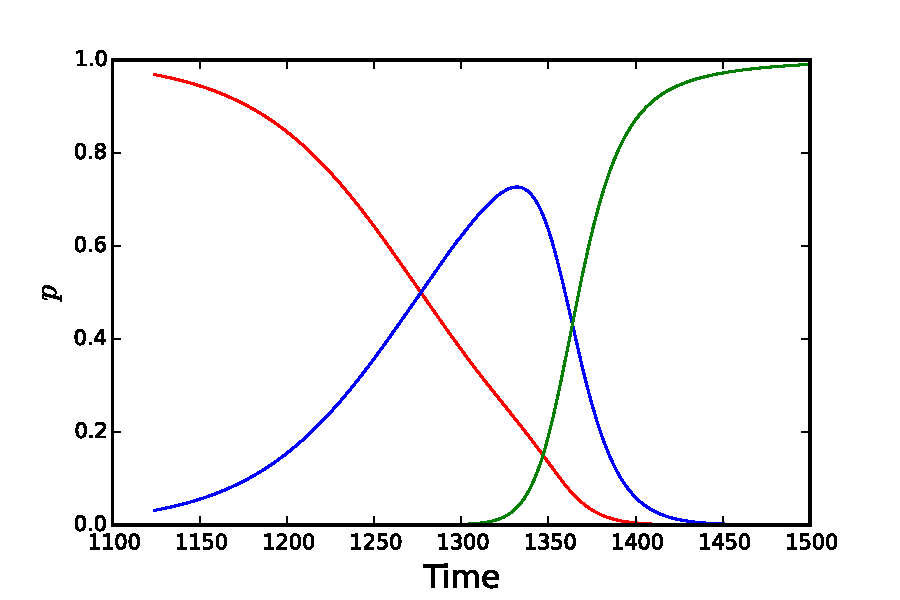
\includegraphics[width=.75\textwidth]{lrp-combined.pdf}\\
\end{center}
	\caption{Proportion of \emph{\textcolor{red}{ne}}, \emph{\textcolor{blue}{ne...not}}, and \emph{\textcolor{green}{not}} predicted by the fitted parameters of the acquisition dynamics}
	\label{lrp-combined}
\end{figure}


\section*{Summary}

In this chapter we presented a model of syntactic acquisition, determined its predicted dynamics in a population over time, and fitted it to data from the formal cycle in Middle English. We found that neither the qualitative nor quantitative criteria for taking acquisition as the cause of the formal cycle were met. All together then, it seems that acquisition cannot be taken as a cause of the formal cycle. If this is indeed the case, then it has important consequences for our understanding of the two transitions of the formal cycle.

Regarding the first transition from \emph{\textcolor{red}{ne}} to \emph{\textcolor{blue}{ne...not}}, if acquisition cannot explain it, then use can. That is, given that this transition coincides with the functional cycle, then the explanation of the functional cycle put forward in the previous chapter is the only and necessarily  the best explanation of the observed transition. Alternative analyses of the grammars underlying the formal cycle may change this, they must be both qualitatively and quantitatively accurate and consistent. 

Regarding the second transition from \emph{\textcolor{blue}{ne...not}} to \emph{\textcolor{green}{not}}, neither acquisition nor use can explain it. The transition does not coincide with another functional cycle, \emph{\textcolor{green}{not}} is not restricted to specific contexts.  This leaves us in the strange position of observing a change without an obvious cause.  Absent some mass coincidence, what are we to make of the second transition of the formal cycle? One possibility is that this second transition is not the result of one mass coincidence, but rather the accumulation of many much smaller coincidences.

To see how this might be the case, consider the fact that the acquisition dynamics only predict a weak form of stability in the expected change of the expected behavior of learners in a population. For example, if we relaxed the assumption regarding the size of the population, then the linguistic environment provided to learners would differ slightly from the limit value. For the second transition, suppose that the proportion of $G_\varnothing$ in the actual linguistic environment is slightly higher than expected due to sampling errors. Now, suppose that it is slightly higher in the next generation as well due to sampling errors. If enough of these small coincidences compound over time, one grammar may replace another without ever having more evidence in favor of it. 

Indeed, this possibility has been extensively studied in population genetics in terms of \emph{genetic drift}. That is, when the selection coefficient is zero $s=0$, as is the case in the second transition of the formal cycle, change can come about due to random sampling. Or, in this case, random changes in the probabilities over grammars learned over time. This means that we the second transition might be the result of a series of small coincidences rather than a single improbable one. In the next chapter we turn to means of testing this possibility.


% Stability
\chapter{Stability (35 pages)}
\label{Stability}


\section{Drift}

\section{Dynamics}

\begin{figure}
\begin{center}
 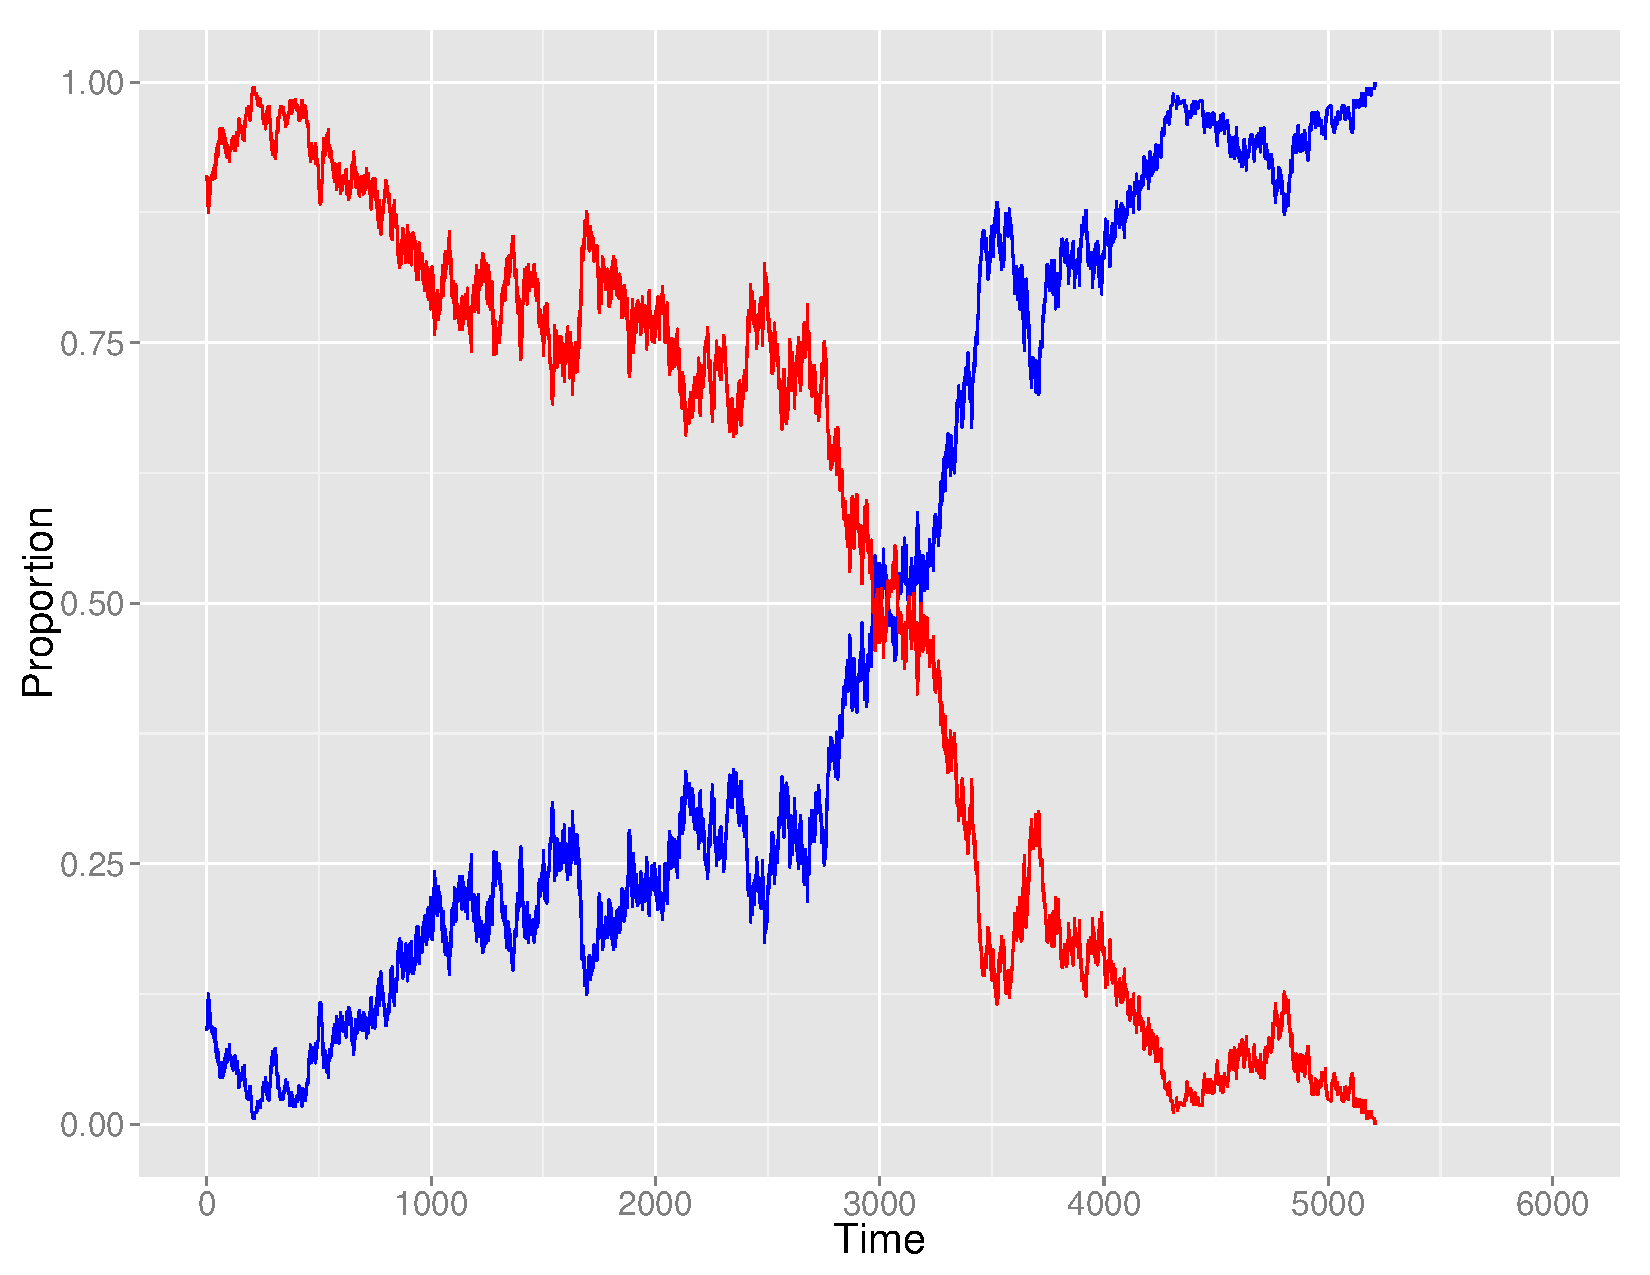
\includegraphics[width=\textwidth]{drift}
\end{center}
	\caption{}
	\label{}
\end{figure}


\begin{figure}
\begin{center}
	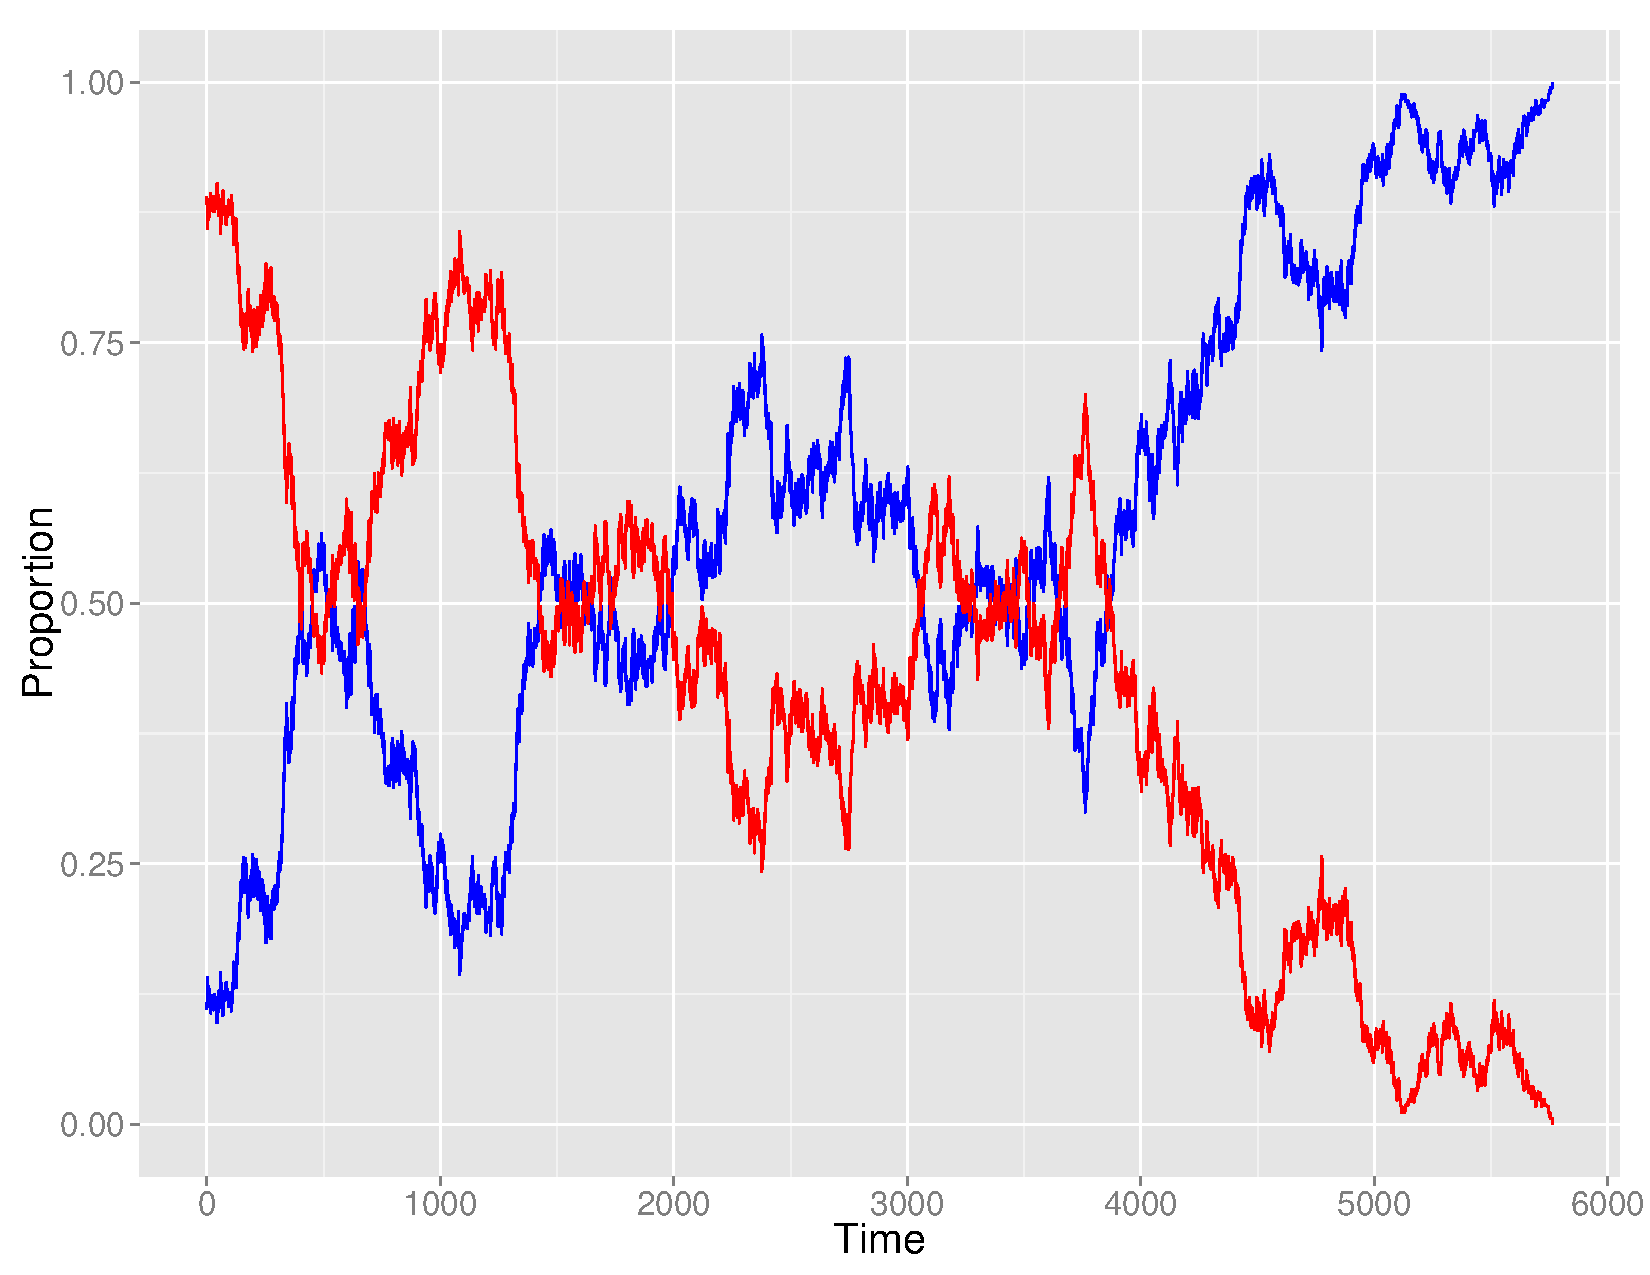
\includegraphics[width=\textwidth]{selection}
\end{center}
	\caption{}
	\label{}
\end{figure}


\section{Data}

Starting in Early Middle English, we find the transition from preverbal to embracing negation taking place. We can trace the proportion of different forms over time as in Figure \ref{neg-three-plot}. Each circle represents tokens in a year. The size of the circle represents the number of tokens negative declaratives. The height of the circle represents the proportion of those instances that are a particular form. Locally-weighted regression lines are fit to these proportions. We see the transition from \textit{\color{red} ne} to \textit{\color{blue} ne...not} starting from around the 12th century. Following close behind, we see the transition from \textit{\color{blue} ne...not} to \textit{\color{green} not} in the 14th century.

\begin{figure}
\centering
     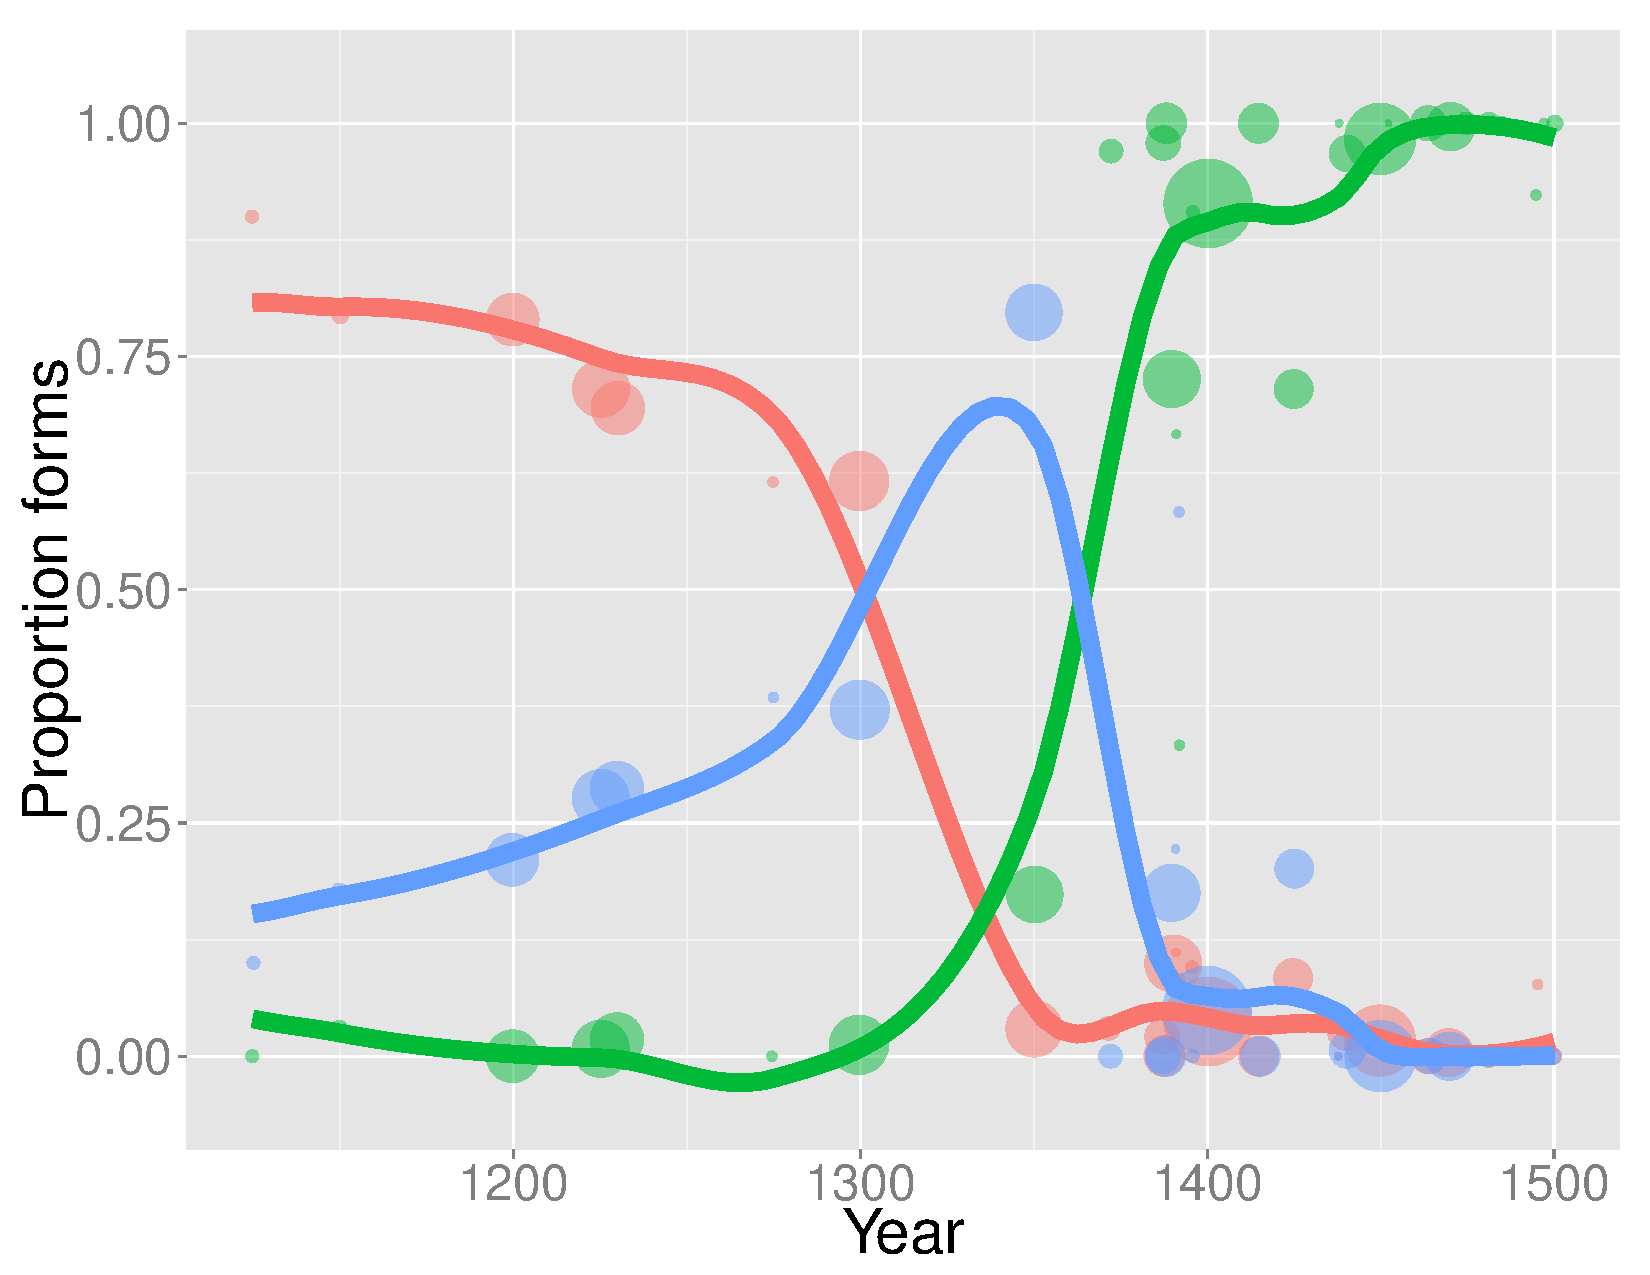
\includegraphics[width=\textwidth]{neg-year-lines.pdf}
\caption{Proportion of forms of negation in Negative Declaratives}
\label{neg-three-plot}
\end{figure}

There are at least two decisions to be made when dealing with the data, which correspond roughly with the ways we'll go about analyzing the data.

First, we have to decide what data should be compared. For example, if we are trying to determine if the first transition is due to selection, should we compare \textit{\color{red} ne} to \textit{\color{blue} ne...not} or should we compare \textit{\color{red} ne} to \textit{\color{blue} ne...not} and \textit{\color{green} not} grouped together? If we do the former, it's pretty clear that the variation beyond 1350 has less to do with the selection of \textit{\color{red} ne} versus \textit{\color{blue} ne...not}, but rather with\textit{\color{green} not} becoming the majority variant. Taking the latter route, and lumping \textit{\color{blue} ne...not} and \textit{\color{green} not} together for the sake of comparison solves this problem.

Second, we have to decide the period of time in which the comparison is being made. This offers another solution to the problem posed above. Namely, if we only compare \textit{\color{red} ne} to \textit{\color{blue} ne...not} prior to 1350 or so we don't have to worry about any noisy  data after that point. There are some natural reasons for choosing a cut-off point. For example, if we are only comparing \textit{\color{red} ne} and \textit{\color{blue} ne...not}, it would seem reasonable to only compare them  when together they constitute the majority of the tokens for a given year. For both transitions, we have the same exact point at 1350, which means we'll be using these tokens for both sets of tests.

We'll try both ways of analyzing the data. First, we'll lump the forms together comparing the pre-verbal to the embracing and post-verbal form, and the pre-verbal and embracing forms to the post-verbal form. We'll do this with all of the data. Second, we'll split the variants, only comparing two forms at a time, before and after 1350.

\subsection{Lumping}

The proportion of \textit{\color{blue} ne...not} and \textit{\color{green} not} forms combined over time can be seen in Figure \ref{lump-plot1}. The results of running the FIT on variable-width bins is shown in Table \ref{lump-table1}. For any binning finer than nine, we find either that an absorption event occurs or there are non-unique ways of binning the data by quantiles.


\begin{figure}
\centering
     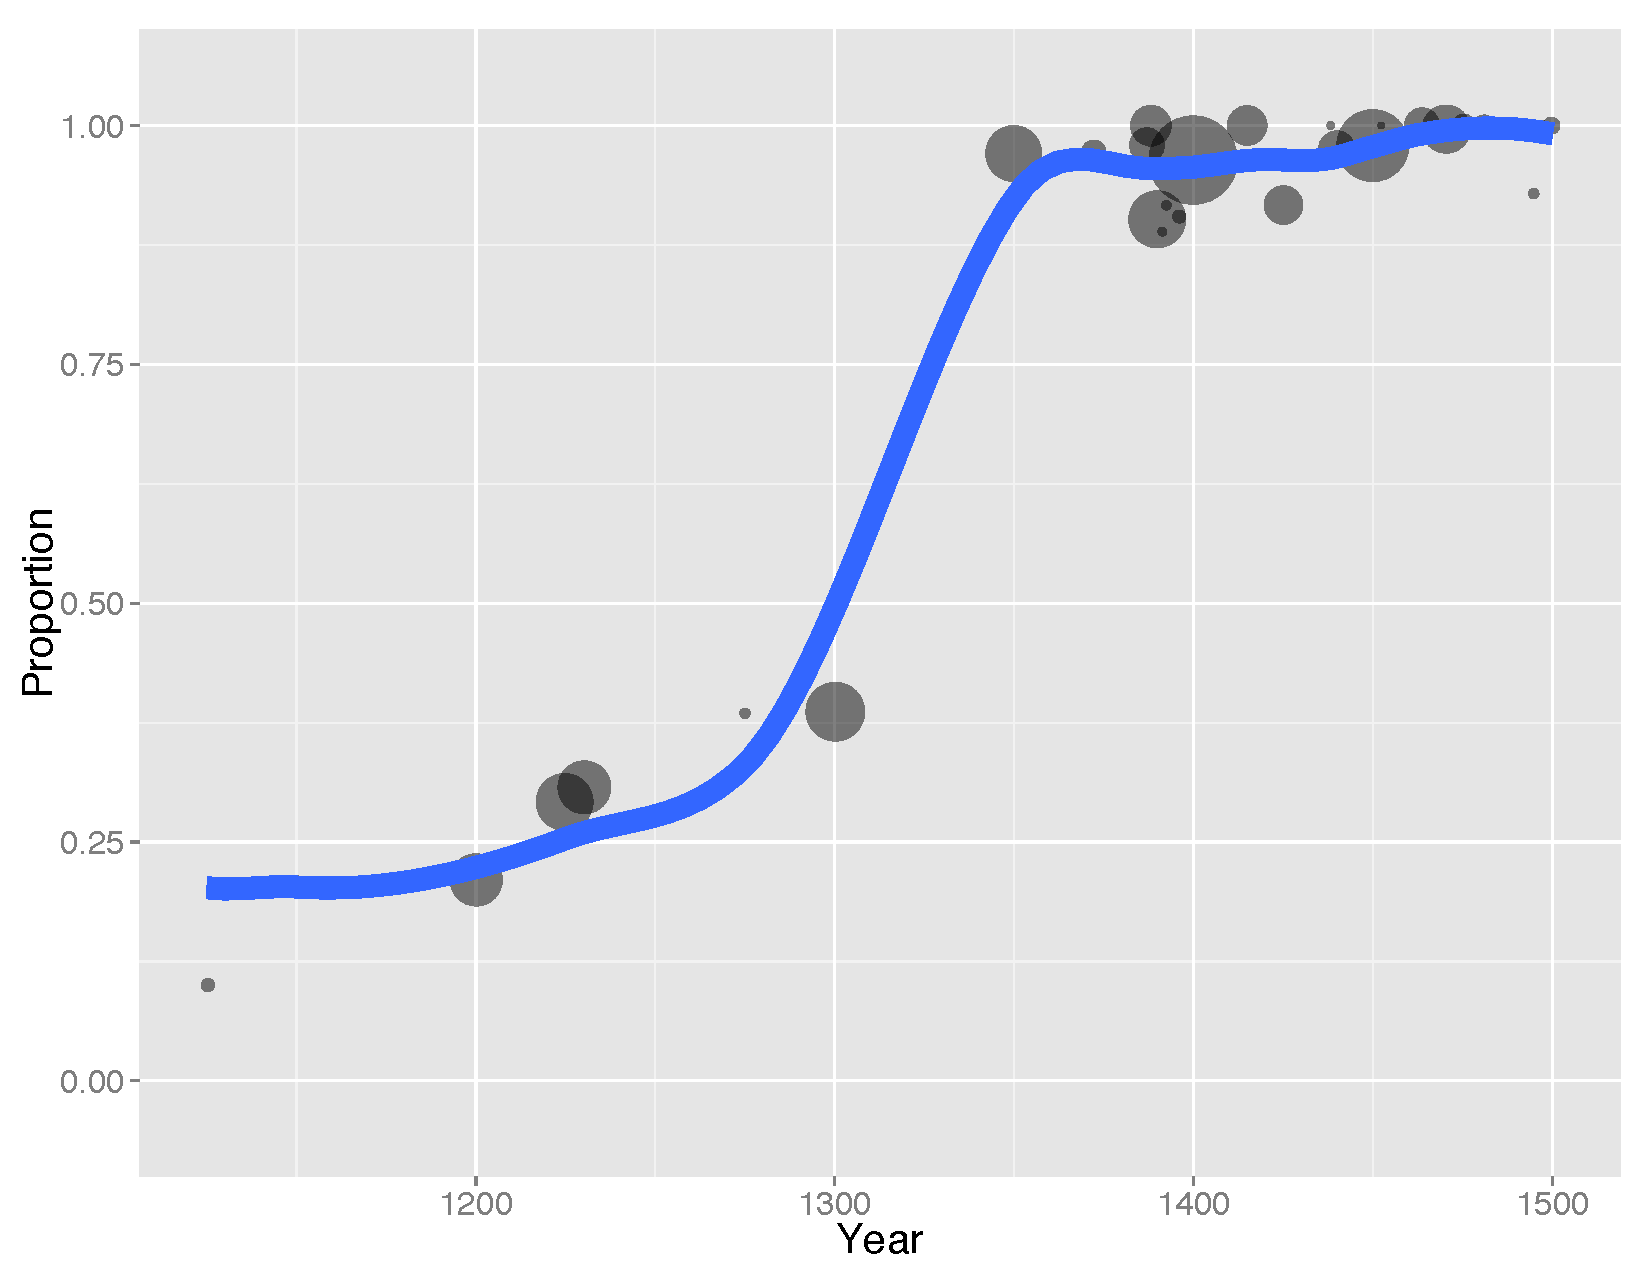
\includegraphics[width=\textwidth]{lump-plot1.pdf}
\caption{Proportion of \textit{\color{blue} ne...not} and \textit{\color{green} not}  versus  \textit{\color{red}  ne} over time}
\label{lump-plot1}
\end{figure}


\begin{table}[ht]
\centering
\begin{tabular}{c  l  r  l  l  l  l   r  r  l l }
  \hline
Bins & ML$s$ & ML$\alpha$ & LRT-P & $\overline{Y}$ & $t_{FI}$ & FIT-P & $\mu$ & $\sigma_n$ & SW-P & WX-P \\ 
  \hline
  4 & 0.02507 & 3270 & 0.000075 & 0.0345 & 1.3269 & 0.1579 & 1368 & 157 & 0.1691 & 0.1250 \\  
  5 & -- & -- & -- & 0.0331 & 2.5445 & 0.0422 & 1094 & 278 & 0.1406 & 0.0625 \\  
  6 & 0.01913 & 15900 & 0.000023 & 0.0278 & 2.6394 & 0.0288 & 912 & 197 & 0.2050 & 0.0312 \\ 
  7 & -- & -- & -- & 0.0238 & 2.4347 & 0.0295 & 781 & 236 & 0.2185 & 0.0313 \\
  8 & -- & -- & -- & 0.0223 & 1.4884 & 0.0936 & 684 & 129 & 0.1619 & 0.0781 \\ 
   \hline
\end{tabular}
\caption{FIT on \textit{\color{red}  ne} versus \textit{\color{blue} ne...not} and \textit{\color{green} not} }
\label{lump-table1}
\end{table}


The proportion of \textit{\color{green} not} forms over time can be seen in Figure \ref{lump-plot2}. The results of running the FIT on variable-width bins is shown in Table \ref{lump-table2}. Again, for any binning finer than nine, we find either that an absorption event occurs or there are non-unique ways of binning the data by quantiles.


\begin{figure}
\centering
     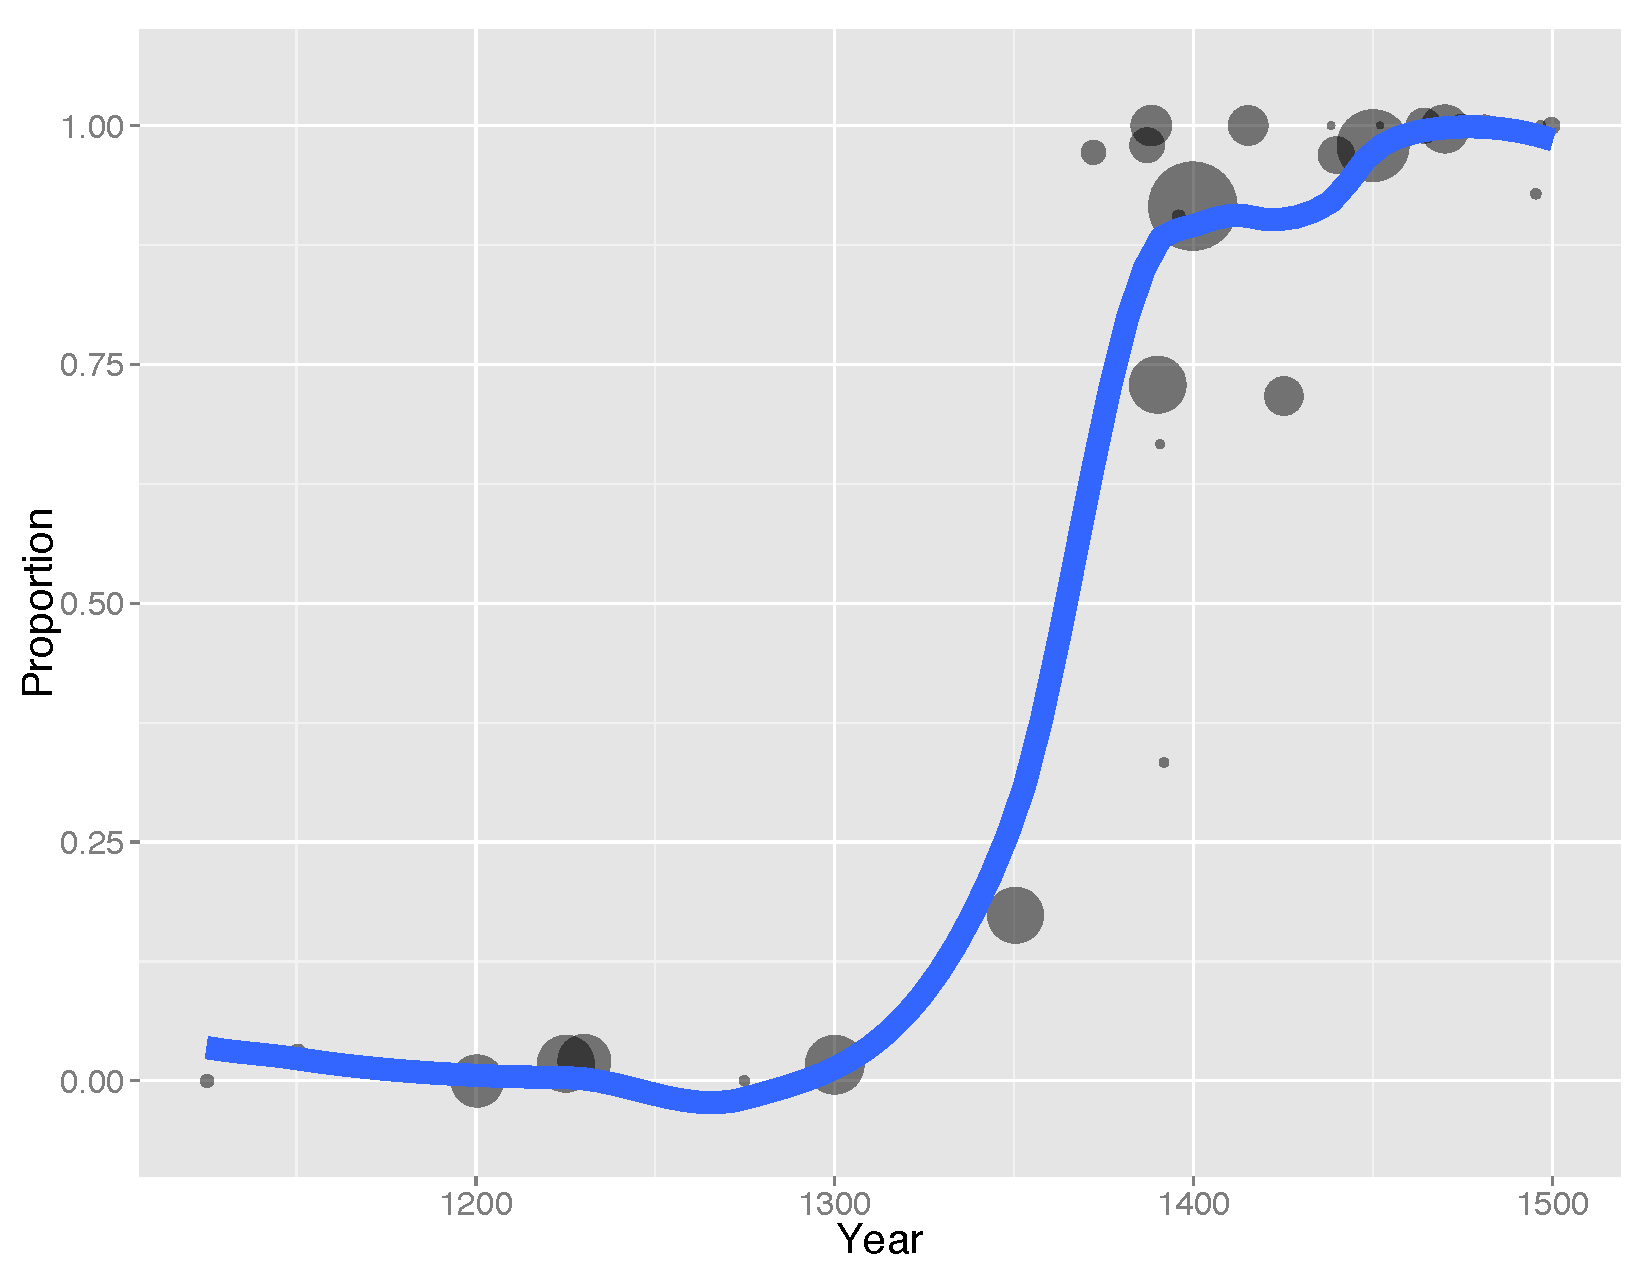
\includegraphics[width=\textwidth]{lump-plot2.pdf}
\caption{Proportion of \textit{\color{green} not} versus \textit{\color{red}  ne} and \textit{\color{blue} ne...not} over time}
\label{lump-plot2}
\end{figure}


\begin{table}[ht]
\centering
\begin{tabular}{c  l  r  l  l  l  l   r  r  l l }
  \hline
Bins & ML$s$ & ML$\alpha$ & LRT-P & $\overline{Y}$ & $t_{FI}$ & FIT-P & $\mu$ & $\sigma_n$ & SW-P & WX-P \\
  \hline
  4 & 0.05791 & 15660 & 0.000045 & 0.1316 & 1.3857 & 0.1501 & 1368 & 157 & 0.1135 & 0.1250 \\
  5 & 0.11907 & 24 & 0.000068 & 0.0825 & 1.9787 & 0.0711 & 1094 & 278 & 0.1300 & 0.0625 \\ 
  6 & -- & -- & --  & 0.0624 & 1.7021 & 0.0820 & 912 & 197 & 0.0052 & 0.0312 \\
  7 & -- & -- & -- & 0.0520 & 1.5250 & 0.0939 & 781 & 236 & 0.0421 & 0.0781 \\ 
  8 & -- & -- & --  & 0.0649 & 1.8516 & 0.0568 & 684 & 129 & 0.0157 & 0.0781 \\    \hline
\end{tabular}
\caption{FIT on \textit{\color{red}  ne} and \textit{\color{blue} ne...not} versus  \textit{\color{green} not} }
\label{lump-table2}
\end{table}


Together, these results suggest the following. First, in some cases we can reject the null hypothesis of drift in favor of selection for the first transition (Table \ref{lump-table1}). Second, we never find sufficient evidence to reject the null hypothesis for the second transition (Table \ref{lump-table2}). Finally, we should note that  the increments for the second transition are not normally distributed as we bin more finely.


%%%%%%%%%%%%%%%%%%%%%%%%%%%%%%%%%%%%%%%%%%
\subsection{Splitting}

If we choose to split the date by date, we limit the number of tokens available and thus how finely we can bin. The proportion of \textit{\color{blue} ne...not}  versus \textit{\color{red} ne} forms over time can be seen in Figure \ref{split-plot1}. The results of running the FIT on variable-width bins is shown in Table \ref{split-table1}. Binning the data into more than six bins is not possible due to either  non-uniquely defined bins, or absorption events. This is not altogether surprising, given that we can only manage eight or so bins with all of the data, as we did above.


\begin{figure}
\centering
     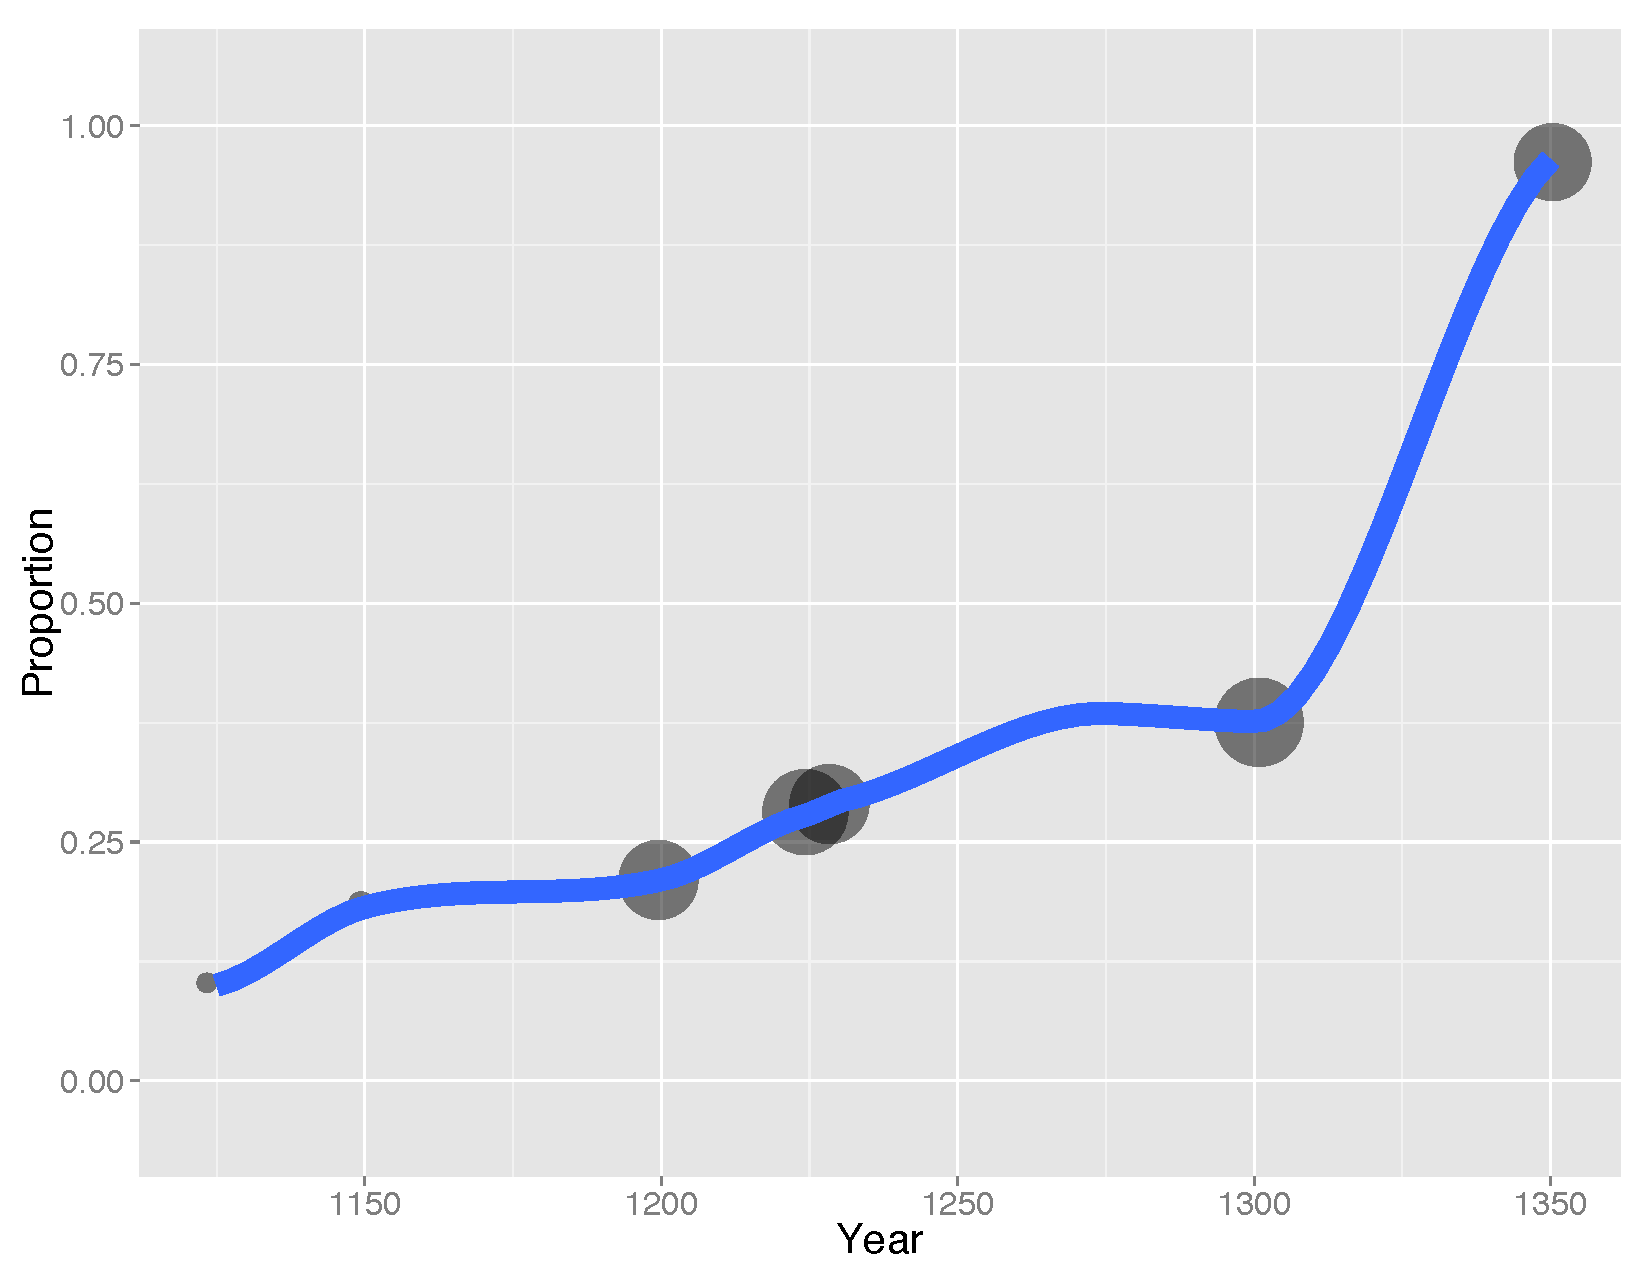
\includegraphics[width=\textwidth]{split-plot1.pdf}
\caption{Proportion of \textit{\color{blue} ne...not}  versus  \textit{\color{red}  ne} until and including 1350}
\label{split-plot1}
\end{figure}

\begin{table}[ht]
\centering
\begin{tabular}{c  l  r  l  l  l  l   r  r  l  l}
  \hline
Bins & ML$s$ & ML$\alpha$ & LRT-P & $\overline{Y}$ & $t_{FI}$ & FIT-P & $\mu$ & $\sigma_n$ & SW-P & WX-P\\ 
  \hline
  4 & 0.02656 & 262 & 0.10 & 0.0480 & 1.5199 & 0.1339 & 454 & 209 & 0.1587 & 0.1250 \\ 
  5 & 0.01140 & 304 & 0.023 & 0.0458 & 1.4588 & 0.1204 & 363 & 38 & 0.0248 & 0.0625 \\
   \hline
\end{tabular}
\caption{FIT on \textit{\color{blue} ne...not}  versus  \textit{\color{red}  ne} until and including 1350}
\label{split-table1}
\end{table}

The proportion of \textit{\color{green} not}  versus \textit{\color{blue} ne...not} forms over time can be seen in Figure \ref{split-plot2}. The results of running the FIT on variable-width bins is shown in Table \ref{split-table2}. Again, binning the data into more than six bins is not possible due to either  non-uniquely defined bins, or absorption events.

\begin{figure}
\centering
     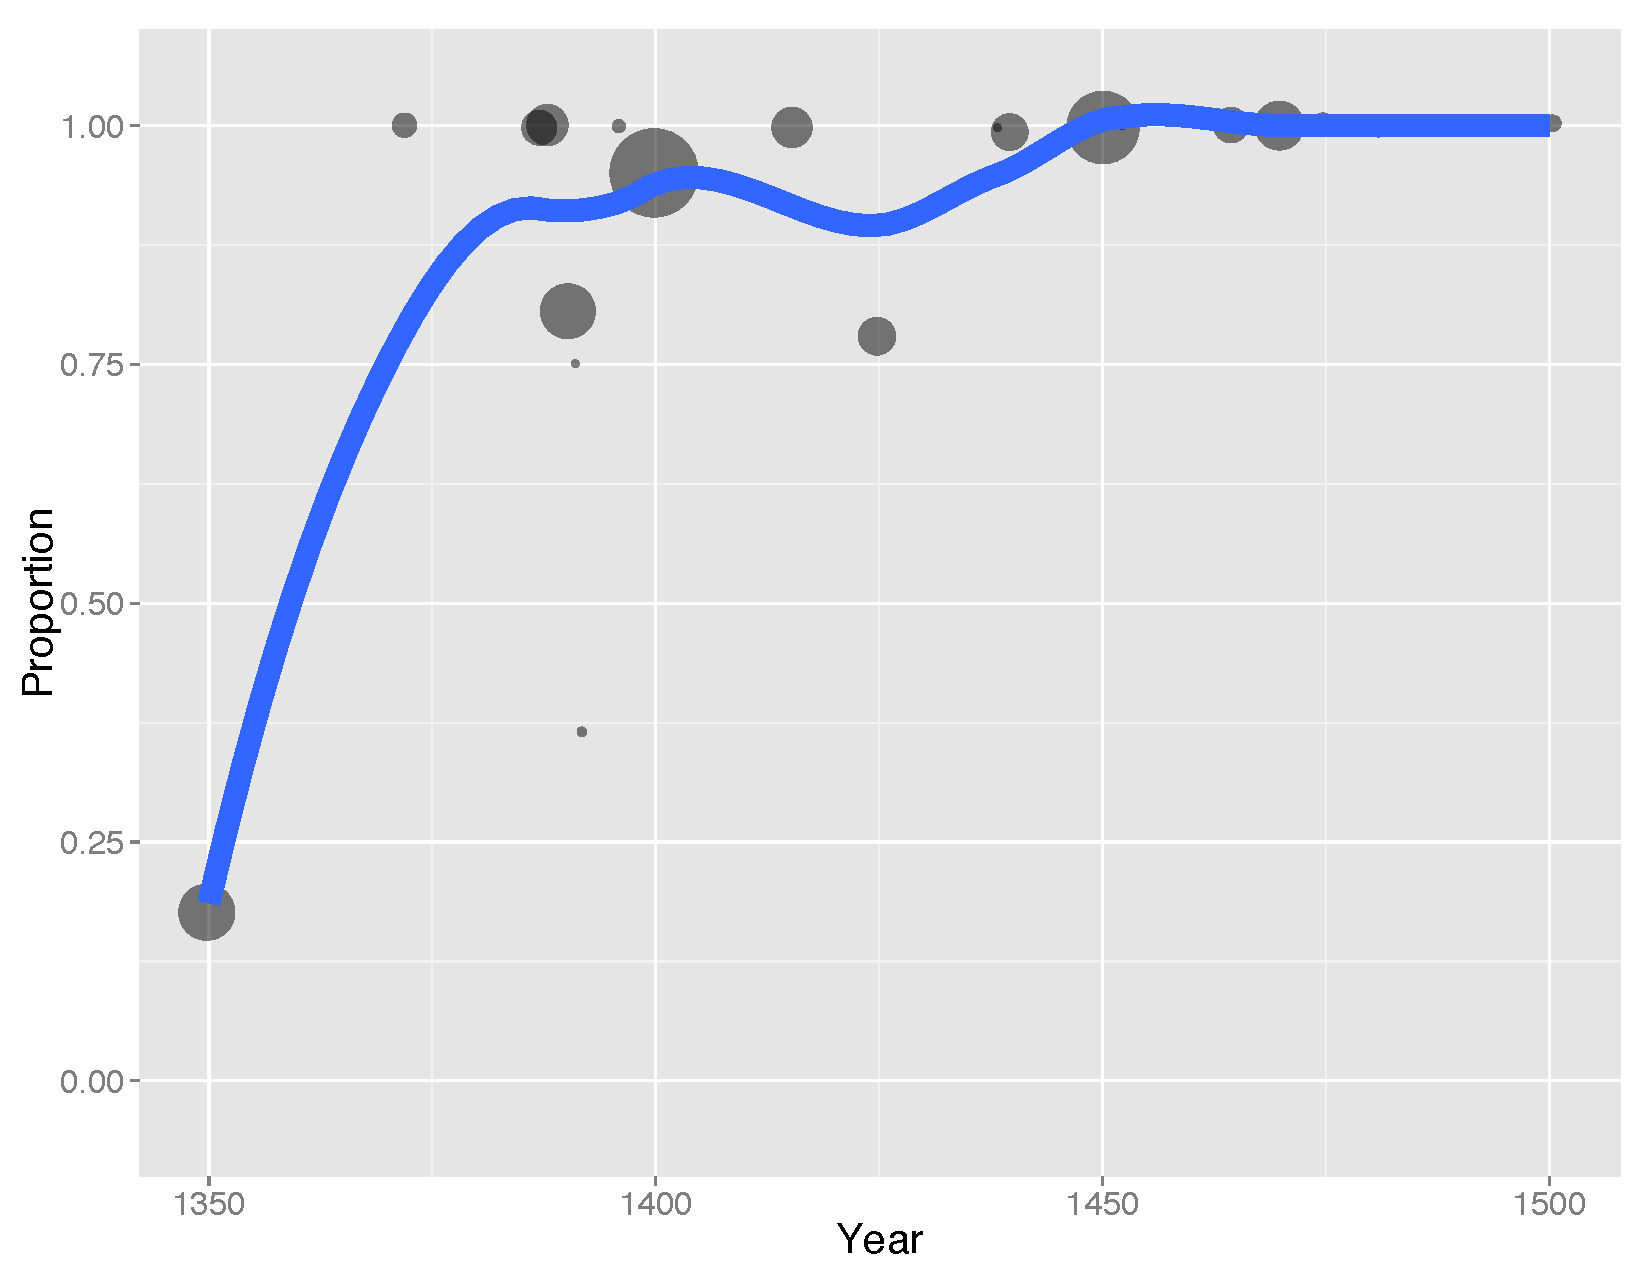
\includegraphics[width=\textwidth]{split-plot2.pdf}
\caption{Proportion of \textit{\color{green} not} versus \textit{\color{blue} ne...not} including and after 1350}
\label{split-plot2}
\end{figure}


\begin{table}[ht]
\centering
\begin{tabular}{c  l  r  l  l  l  l   r  r  l  l}
  \hline
Bins & ML$s$ & ML$\alpha$ & LRT-P & $\overline{Y}$ & $t_{FI}$ & FIT-P & $\mu$ & $\sigma_n$ & SW-P & WX-P \\ 
  \hline
  4 & 0.06728 & 1423 & 0.000086 & 0.0377 & 1.7370 & 0.1123 & 953 & 235 & 0.1218 & 0.1250 \\ 
  5 & -- & -- & -- & 0.0329 & 1.5942 & 0.1046 & 763 & 339 & 0.5138 & 0.1875 \\ 
  \hline
\end{tabular}
\caption{FIT on \textit{\color{green} not} versus \textit{\color{blue} ne...not} including and after 1350}
\label{split-table2}
\end{table}


\section{Dates}
\label{Dates}

Given that we have limited data we can't bin too finely, otherwise we run into one of two problems. Either we have an absorption event where all of the tokens are of one kind or another, or we have non-uniquely defined quantiles, we have no motivated way of splitting things up. An important question is whether these dates reflect information or are simply artifacts of uncertainty. That is, are documents dated 1225 really from 1225, or are they simply our best guess using quarter centuries?

Figure \ref{auth-plot} shows the number of documents per year. There are two important things to note. First, the documents are clustered around salient dates, roughly every quarter century. Second, we have more documents as time goes by and these are less concentrated at quarter century marks.

\begin{figure}
\centering
     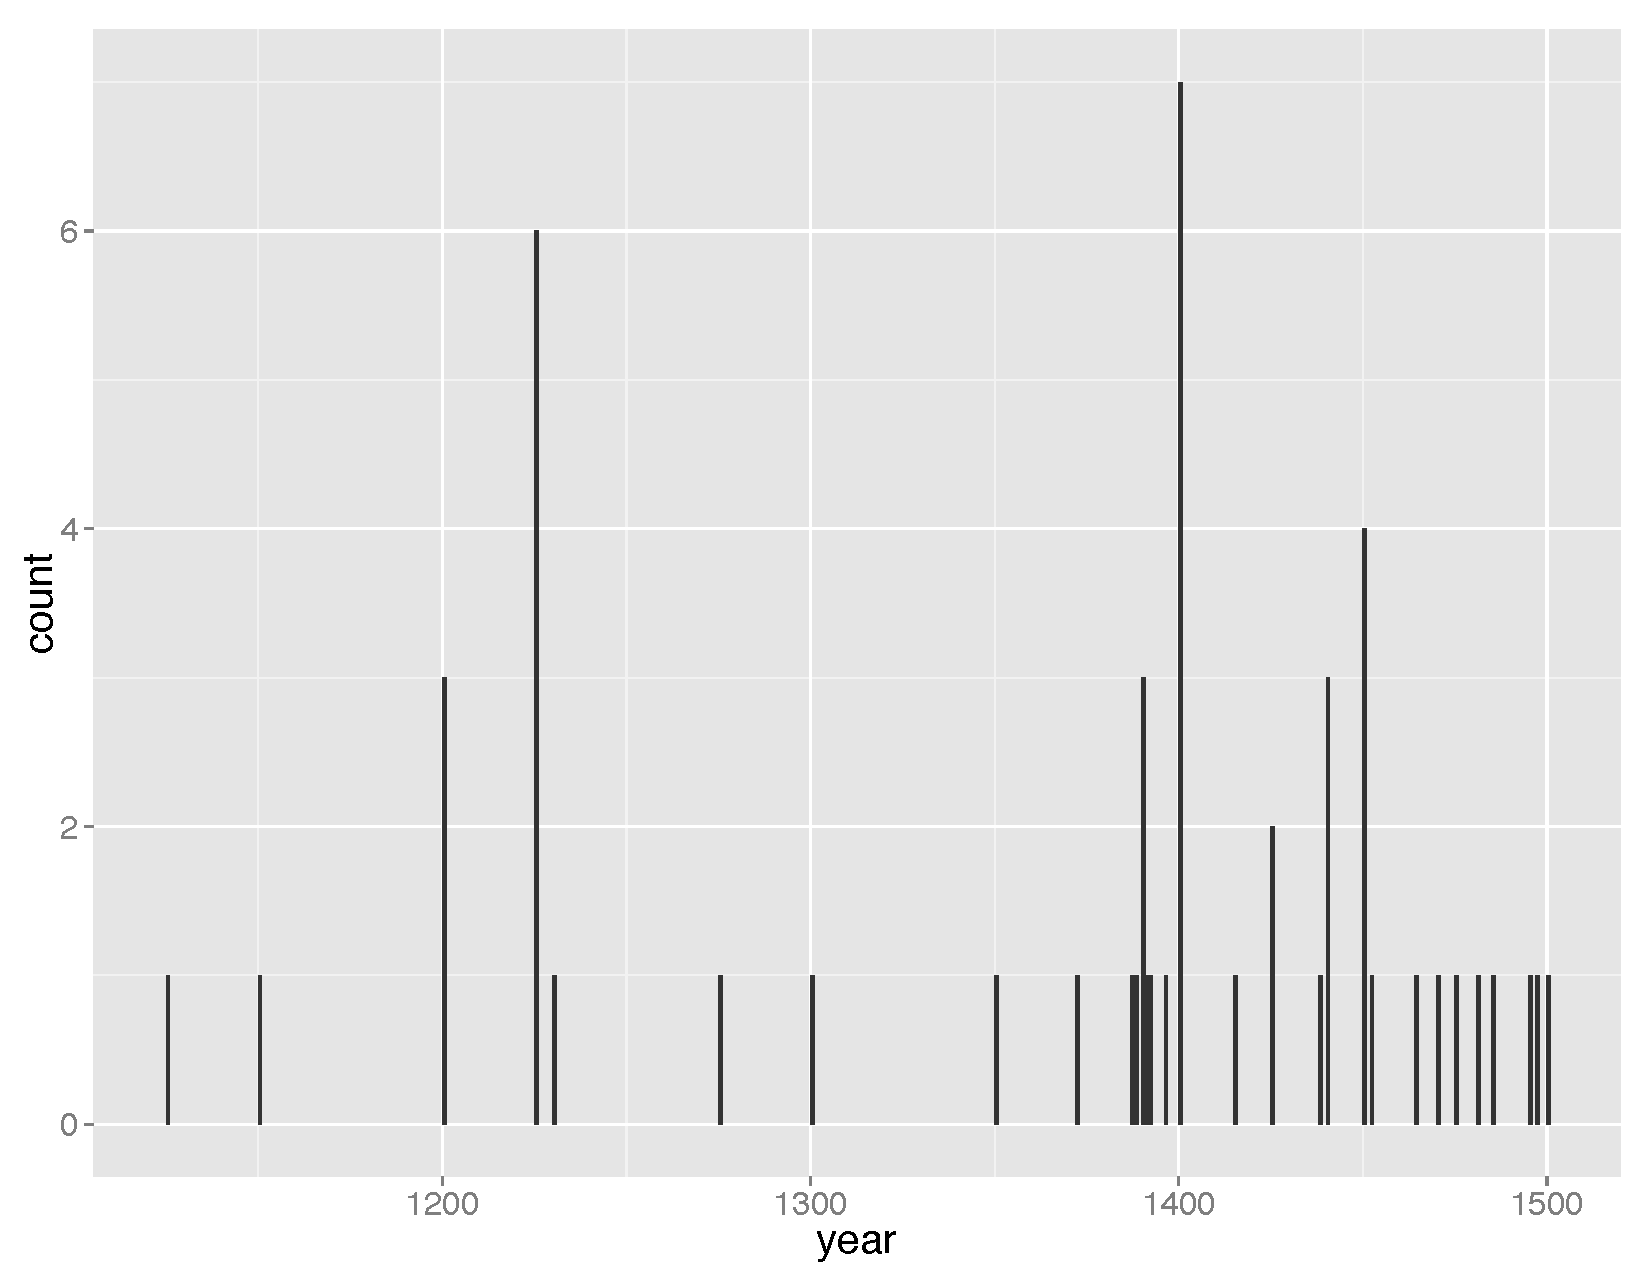
\includegraphics[width=\textwidth]{auth-plot.pdf}
\caption{Count of documents by year}
\label{auth-plot}
\end{figure}

We can try to adjust for the possibility that dates clustered around quarter century marks are artifacts rather than information by adding a small amount of noise to the date for each document. The amount of noise is uniformly distributed over $[-.5, .5 ]$. This means that documents clustered around quarter centuries will be randomly disaggregated, but no documents that are dated in unique years will be swapped in order. The upside of this is that we can simulate what would happen if we had more information about the dates of the documents.

\subsection{Lumping}

Disaggregating the data in this way allows us to bin more finely, but it doesn't shed too much more light on either transition, as we see in Tables \ref{jitter-lump-table1} and \ref{jitter-lump-table2}. For the most part, the resolution we gain from disaggregating the data is counterbalanced by the increments not being normally distributed

%\begin{figure}
%\centering
%     \includegraphics[width=\textwidth]{jitter-lump-plot1.pdf}
%\caption{Proportion of \textit{\color{blue} ne...not} and \textit{\color{green} not}  versus  \textit{\color{red}  ne} over time with jittered dates}
%\label{jitter-lump-plot1}
%\end{figure}

%JITTER-LUMP-FIRSTq04.out:MLS = 0.02491
%JITTER-LUMP-FIRSTq06.out:MLS = 0.01930
%JITTER-LUMP-FIRSTq07.out:MLS = 0.02590
%JITTER-LUMP-FIRSTq08.out:MLS = 0.03585
%JITTER-LUMP-FIRSTq09.out:MLS = 0.03521
%JITTER-LUMP-FIRSTq11.out:MLS = 0.02261
%
%JITTER-LUMP-FIRSTq04.out:MLALPHA = 3347
%JITTER-LUMP-FIRSTq06.out:MLALPHA = 15650
%JITTER-LUMP-FIRSTq07.out:MLALPHA = 680
%JITTER-LUMP-FIRSTq08.out:MLALPHA = 138
%JITTER-LUMP-FIRSTq09.out:MLALPHA = 47
%JITTER-LUMP-FIRSTq11.out:MLALPHA = 663
%
%JITTER-LUMP-FIRSTq04.out:CHI2P = 0.000077
%JITTER-LUMP-FIRSTq06.out:CHI2P = 0.000023
%JITTER-LUMP-FIRSTq07.out:CHI2P = 0.000033
%JITTER-LUMP-FIRSTq08.out:CHI2P = 0.000022
%JITTER-LUMP-FIRSTq09.out:CHI2P = 0.000022
%JITTER-LUMP-FIRSTq11.out:CHI2P = 0.0010


\begin{table}[ht]
\centering
\begin{tabular}{c  l  r  l  l  l  l   r  r  l  l }
  \hline
Bins & ML$s$ & ML$\alpha$ & LRT-P & $\overline{Y}$ & $t_{FI}$ & FIT-P & $\mu$ & $\sigma_n$ & SW-P  & WX-P\\ 
  \hline
  4 & 0.02491 & 3347 & 0.000077 & 0.0346 & 1.3256 & 0.1581 & 1368 & 157 & 0.1684 & 0.1250 \\ 
  5 & -- & -- & -- & 0.0320 & 2.3890 & 0.0484 & 1094 & 72 & 0.1748 & 0.0625 \\
  6 & 0.01930 & 15650 & 0.000023 & 0.0279 & 2.6530 & 0.0284 & 912 & 206 & 0.1479 & 0.0312 \\ 
  7 & 0.02590 & 680 & 0.000033 & 0.0200 & 1.4793 & 0.0996 & 781 & 206 & 0.3617 & 0.1094 \\  
  8 & 0.03585 & 138 & 0.000022 & 0.0226 & 1.4898 & 0.0934 & 684 & 84 & 0.2502 & 0.0781 \\ 
  9 & 0.03521 & 47 & 0.000022 & 0.0195 & 1.3623 & 0.1077 & 608 & 190 & 0.0009 & 0.1250 \\ 
  10 & -- & -- & -- & 0.0123 & 0.6530 & 0.2660 & 547 & 111 & 0.0397 & 0.1797 \\  
  11 & 0.02261 & 663 & 0.0010 & -- & -- & -- & -- & -- & --\\ 
  12 & -- & -- & --  &  0.0133 & 0.8299 & 0.2129 & 456 & 129 &  0.0675 & 0.0615\\
  13 & -- & -- & --  &  0.0114 & 0.7063 & 0.2473 & 420 & 127 &  0.3521 & 0.1901\\
  14 & -- & -- & --  &  0.0121 & 0.8980 & 0.1934 & 390 & 154 &  0.0828 & 0.0549\\
  15 & -- & -- & --  &  0.0072 & 0.4920 & 0.3154 & 364 & 74   &  0.1232 & 0.1478\\
   \hline
\end{tabular}
\caption{FIT on \textit{\color{red}  ne} versus \textit{\color{blue} ne...not} and \textit{\color{green} not} with jittered dates}
\label{jitter-lump-table1}
\end{table}


\begin{figure}
\centering
     \includegraphics[width=\textwidth]{jitter-lump-first-increments.pdf}
\caption{Distribution of increments for  comparison of \textit{\color{blue} ne...not} and \textit{\color{green} not}  versus  \textit{\color{red}  ne} over time with jittered dates}
\label{jitter-lump-first-increments}
\end{figure}




%\begin{figure}
%\centering
%     \includegraphics[width=\textwidth]{jitter-lump-plot2.pdf}
%\caption{Proportion of \textit{\color{green} not} versus \textit{\color{red}  ne} and \textit{\color{blue} ne...not} over time with jittered dates}
%\label{jitter-lump-plot2}
%\end{figure}

%JITTER-LUMP-SECONDq07.out:MLS = 0.03829
%JITTER-LUMP-SECONDq09.out:MLS = 0.03523
%JITTER-LUMP-SECONDq10.out:MLS = 0.03250
%JITTER-LUMP-SECONDq13.out:MLS = 0.07745
%JITTER-LUMP-SECONDq15.out:MLS = 0.00458
%
%JITTER-LUMP-SECONDq07.out:MLALPHA = 112
%JITTER-LUMP-SECONDq09.out:MLALPHA = 224
%JITTER-LUMP-SECONDq10.out:MLALPHA = 102
%JITTER-LUMP-SECONDq13.out:MLALPHA = $\infty$
%JITTER-LUMP-SECONDq15.out:MLALPHA = 9
%
%JITTER-LUMP-SECONDq07.out:CHI2P = 0.00028
%JITTER-LUMP-SECONDq09.out:CHI2P = 0.000050
%JITTER-LUMP-SECONDq10.out:CHI2P = 0.00090
%JITTER-LUMP-SECONDq13.out:CHI2P = --
%JITTER-LUMP-SECONDq15.out:CHI2P = --


\begin{table}[ht]
\centering
\begin{tabular}{c  l  r  l  l  l  l   r  r  l  l}
  \hline
Bins & ML$s$ & ML$\alpha$ & LRT-P & $\overline{Y}$ & $t_{FI}$ & FIT-P & $\mu$ & $\sigma_n$ & SW-P  & WX-P\\ 
  \hline
  4 & -- & -- & -- & 0.1315 & 1.3848 & 0.1502 & 1368 & 145 & 0.1135 & 0.1250 \\ 
  5 & -- & -- & -- & 0.0812 & 1.9173 & 0.0755 & 1094 & 77 & 0.1333 & 0.0625\\ 
  6 & -- & -- & -- & 0.0621 & 1.7023 & 0.0820 & 912 & 164 & 0.0065 & 0.0312\\ 
  7 & 0.03829 & 112 & 0.00028 & 0.0428 & 0.9306 & 0.1974 & 781 & 204 & 0.2285 & 0.1563\\ 
  8 & -- & -- & -- & 0.0656 & 1.7613 & 0.0643 & 684 & 78 & 0.0507 & 0.0391\\ 
  9 & 0.03523 & 224 & 0.000050 & 0.0463 & 1.6840 & 0.0680 & 608 & 193 & 0.0633 & 0.0547\\ 
  10 & 0.03250 & 102 & 0.00090 & 0.0137 & 0.2563 & 0.4021 & 547 & 128 & 0.0735 & 0.1504\\  
  11 & -- & -- & -- & -- & -- & -- & -- & -- & -- & --\\  
  12 & -- & -- & -- & 0.0120 & 0.2760 & 0.3940 & 456 & 129 & 0.0674 & 0.2065\\
  13 & 0.07745 & $\infty$ & -- & 0.0274 & 0.9516 & 0.1808 & 420 & 127 & 0.9002 & 0.2592\\
  14 & -- & -- & -- & 0.0149 & 0.3916 & 0.3511 & 390 & 154 & 0.0614 & 0.2274\\
  15 & 0.00458 & 9 & -- & 0.0042 & 0.1146 & 0.4552 & 364 & 74   & 0.0273 & 0.1629\\
  \hline
  \end{tabular}
\caption{FIT on \textit{\color{red}  ne} and \textit{\color{blue} ne...not} versus  \textit{\color{green} not} with jittered dates}
\label{jitter-lump-table2}
\end{table}

\begin{figure}
\centering
     \includegraphics[width=\textwidth]{jitter-lump-second-increments.pdf}
\caption{Distribution of increments for  comparison of \textit{\color{red}  ne} and \textit{\color{blue} ne...not} versus  \textit{\color{green} not} over time with jittered dates}
\label{jitter-lump-second-increments}
\end{figure}


\subsection{Splitting}

Again, disaggregating the data in this way allows us to bin more finely, but only in the case of the second transition. However, we still don't find sufficient evidence to reject the null hypothesis of drift, as we can see in Tables \ref{jitter-split-table1} and \ref{jitter-split-table2}.

 
 
\begin{figure}
\centering
     \includegraphics[width=\textwidth]{jitter-split-plot1.pdf}
\caption{Proportion of \textit{\color{blue} ne...not} and \textit{\color{green} not}  versus  \textit{\color{red}  ne} over time with jittered dates}
\label{jitter-split-plot1}
\end{figure}

%JITTER-SPLIT-FIRSTq04.out:MLS = 0.02697
%JITTER-SPLIT-FIRSTq05.out:MLS = 0.01140
%
%JITTER-SPLIT-FIRSTq04.out:MLALPHA = 284
%JITTER-SPLIT-FIRSTq05.out:MLALPHA = 304
%
%JITTER-SPLIT-FIRSTq04.out:CHI2P = 0.092
%JITTER-SPLIT-FIRSTq05.out:CHI2P = 0.23

\begin{table}[ht]
\centering
\begin{tabular}{c  l  r  l  l  l  l   r  r  l  }
  \hline
Bins & ML$s$ & ML$\alpha$ & LRT-P & $\overline{Y}$ & $t_{FI}$ & FIT-P & $\mu$ & $\sigma_n$ & SW-P \\ 
  \hline
  4 & 0.02697 & 284 & 0.092 & 0.0497 & 1.6164 & 0.1237 & 454 & 126 & 0.1687 \\ 
  5 & 0.01140 & 304 & 0.23 & 0.0458 & 1.4588 & 0.1204 & 363 & 38 & 0.0248 \\    \hline
\end{tabular}
\caption{FIT on \textit{\color{red}  ne} versus \textit{\color{blue} ne...not} with jittered dates}
\label{jitter-split-table1}
\end{table}


\begin{figure}
\centering
     \includegraphics[width=\textwidth]{jitter-split-plot2.pdf}
\caption{Proportion of \textit{\color{green} not} versus \textit{\color{red}  ne} and \textit{\color{blue} ne...not} over time with jittered dates}
\label{jitter-split-plot2}
\end{figure}

%JITTER-SPLIT-SECONDq04.out:MLS = 0.05791
%JITTER-SPLIT-SECONDq05.out:MLS = 0.11907
%
%JITTER-SPLIT-SECONDq04.out:MLALPHA = 15660
%JITTER-SPLIT-SECONDq05.out:MLALPHA = 24
%
%JITTER-SPLIT-SECONDq04.out:CHI2P = 0.000045
%JITTER-SPLIT-SECONDq05.out:CHI2P = 0.000068
%

\begin{table}[ht]
\centering
\begin{tabular}{c  l  r  l  l  l  l   r  r  l  }
  \hline
Bins & ML$s$ & ML$\alpha$ & LRT-P & $\overline{Y}$ & $t_{FI}$ & FIT-P & $\mu$ & $\sigma_n$ & SW-P \\ 
  \hline
  4 & 0.05791 & 15660 & 0.000045 & 0.0391 & 2.2066 & 0.0790 & 953 & 181 & 0.1385 \\ 
  5 & 0.11907 & 24 & 0.000068 & 0.0335 & 1.6935 & 0.0945 & 763 & 144 & 0.4040 \\ 
  6 & -- & -- & -- & -- & 2.1307 & 0.0615 & 635 & 100 & 0.2593 \\ 
  7 & -- & -- & -- & -- & 1.6475 & 0.0874 & 545 & 65 & 0.6893 \\ 
  8 & -- & -- & -- & -- & 1.0583 & 0.1692 & 476 & 211 & 0.0682 \\ 
  9 & -- & -- & -- & -- & -0.0420 & 0.5159 & 423 & 111 & 0.5804 \\   \hline
  \end{tabular}
\caption{FIT on \textit{\color{blue} ne...not} versus  \textit{\color{green} not} with jittered dates}
\label{jitter-split-table2}
\end{table}


%\section{Introduction}
%
%Here we'll compare different ways of binning time series data to test for drifts versus selection. The goal will be to motivate  a particular method for binning the data. We'll compare fixed- and variable-width bins for the $\chi^2$ likelihood ratio test (LRT) and the fitness increment test (FIT). Before moving on to the data and the particular methods, we note two sets of constraints on how we bin the data which are motivated by the results in \cite{feder-etal2014}. 
%
%The first set of constraints are \textbf{theoretical} and have to do with what we are calculating. For example, to jointly estimate the maximum likelihood population size and selection coefficient for the LRT we need at least three data points and thus at least three bins (p.511). Likewise, to perform the FIT we need at least two increments to compute the test statistic and thus at least three bins (p.512). In the opposite direction, we can't bin the data too finely because the fitness increment test is only appropriate if no absorption event occurs prior to the last bin (p.516). No document without variation between the forms can constitute its own bin, unless it happens to be the last document. Additionally, we cannot have more bins than there are uniquely-dated documents. Otherwise we'll end up with empty bins, which will render the FIT undefined. Finally, the Gaussian approximation of the diffusion process rests on the assumption of normality both in the movement of allele frequency and the distribution 
%of the rescaled fitness increments. We'll need at least three increments, and thus four bins to test for normality.
%
%The second set of constraints are \textbf{practical} and have to do with the power of the tests we are calculating, in particular, the power of the FIT. When samples are drawn at equal intervals, the power of the FIT grows weakly with and increase in the number of sampled time points (p.514, Figure 2), which is reproduced here in Figure \ref{power}. This suggests that the more bins we have the better. However, with noisy sampling at equally-spaced intervals, the statistical power of the FIT decreases with fewer samples drawn (p.517, Figure 5), which is reproduced in Figure \ref{power-sample}. Given that historical data are limited, this suggests that the fewer bins we have the better. While historical documents are not ``sampled'' at equal intervals, this second set of constraints suggests that we want a balance between how many bins we have and the number of data points per bin that we have. 
%
%\begin{figure}
%\centering
%     \includegraphics[width=3in]{power.png}
%\caption{Power of FIT for $L = 5, 10, 50$ for various levels of selection pressure $Ns$}
%\label{power}
%\end{figure}
%
%\begin{figure}
%\centering
%     \includegraphics[width=3in]{power-sample.png}
%\caption{Power of FIT for $L = 10$ for various levels of selection pressure $Ns$ with samples of size $n = 100, 1000, 10000$}
%\label{power-sample}
%\end{figure}
%
%
%
%Our goal will be to find a method of binning that abides by the first set of constraints, while striking a balance between the competing demands of the second set of constraints. We begin in Section \ref{do-support} with a  brief overview of the \emph{do}-support data and compare results for fixed- and variable-width bins.
%
%\section{\emph{do}-support}
%\label{do-support}
%
%The general trajectory of the change in \emph{do}-support is shown in Figure \ref{do-support-sub}. In what follows, we'll pool the data across contexts, leaving investigations of individual contexts for future exploration.
%
%\begin{figure}
%\centering
%     \includegraphics[width=\textwidth]{do-support-drift.pdf}
%\caption{Proportion of \emph{do}-support in coherent contexts}
%\label{do-support-sub}
%\end{figure}
%
%In what follows, we'll include all tokens from the very instance of \emph{do}-support onwards. The first instance occurs in 1440. Originally, I'd used only those tokens from 1500 to 1900, to allow an easy comparison between fixed-width bins across contexts (e.g. negative declaratives versus negative imperatives, etc.). However, since we are not examining or comparing across contexts, or using fixed-width bins, it makes far more sense to include as much data as possible.  In fact, doing so allows us to add around seven hundred more tokens to our analysis.  In data from 1440 on, we have a little more than 11,000 tokens with 307 years represented, as well as roughly 2,500 individual documents by 600 authors.\footnote{The estimate of authors slightly low. Around 50 authors are labeled together.}
%
%We can get a general sense of the distribution of tokens over time and the difference between fixed- and variable-width bins in Figure \ref{do-compare-all}. The count of tokens per bin is shown for both fixed-width (gray) and variable-width bins (white). The variable-width bins are quantiles, where the number of tokens is as close to even across bins as possible.\footnote{There are several algorithms for calculating quantiles. For now, I've simply used the default, but this is something to explored. This might be particularly relevant when the quantiles are not uniquely defined by a particular algorithm.} In the upper-left, where the number of bins $n=4$, we see that the fixed-width bins vary rather widely, whereas the variable-width quantiles quite a bit less, exactly as we would expect.
%
%\begin{figure}
%\centering
%     \includegraphics[width=\textwidth]{do-compare-all.pdf}
%\caption{Count of tokens per bin for fixed- (gray) and variable width bins (white) for $n = 4,5,10,20$}
%\label{do-compare-all}
%\end{figure}
%
%Figure \ref{do-compare-all} also shows the mean number of tokens  per bin $\mu$, the standard deviation of the fixed-width bins $\sigma_n$, and the standard deviation of the variable-width bins $\sigma_q$. As the number of bins increases, the average number of tokens per bin decreases, the variance of the number of tokens per fixed-width bins decreases, and the variance of the number of tokens per variable-width bins increases.
%
%
%\subsection{Fixed-Width Bins}
%
%We start with all of the data pooled together and bin from four to an increasing number of bins. Given that there are several thousand tokens of potential instances of \emph{do}-support, we could reasonably partition the data rather finely. Table \ref{do-n-bin-all} gives the results for different numbers of bins.
%
%We report the results for the $\chi^2$  LRT, including the output from \emph{tsinfer} where possible. We also report the results of the FIT, including the average fitness increment $\overline{Y}$, and the test statistic $t_{FI}$,  along with the results of the \href{http://en.wikipedia.org/wiki/Shapiro\%E2\%80\%93Wilk_test}{Shapiro-Wilk Test}.\footnote{The null hypothesis for the Shapiro-Wilk test is that the rescaled fitness increments are normally distributed, as is assumed by the Gaussian approximation to the diffusion process. When the P-value of the test is below the specified value, we reject the null hypothesis.} Finally, we report the mean number of tokens per bin and the standard deviation of the number of tokens per bin.
%
%%\begin{table}[ht]
%%     \begin{center}
%%     \begin{tabular}{ c  l  r  l  l  l  l  l}
%%      \hline
%%       Bins & ML$s$   & ML$\alpha$ & $\chi^2$ LRT-P   & FIT-P 		& SW-P 		& $\mu$ & $\sigma_n$\\ \hline
%%       4    & 0.01432 & 4034       & .0036 	      & 0.04914006	& 0.8147933	& 2613 & 1695\\
%%       5    & 0.01319 & 3324       & .0043 	      & 0.04653923	& 0.7577887	& 2090 & 1199\\
%%       6    & 0.01560 & 4317       & .00037	      & 0.02175		& 0.2364045	& 1742 & 1159\\
%%       7    & 0.01557 & 4820       & .00015	      & 0.008755987	& 0.4168814	& 1493 & 810\\
%%       8    & 0.01998 & 694        & .0016	      & 0.05299804	& 0.7387052	& 1307 & 856\\
%%       9    & 0.02750 & $\infty$   & .000021	      & 0.03056291	& 0.1602431	& 1161 & 731\\ \hdashline
%%       10   & --      & --         & --  	      & 0.08984853	& 0.005722805	& 1045         & 697\\ 
%%       11   & 0.01742 & 749        & .0037  	      & 0.0735404	& 0.4267124	& 950   & 569\\ 
%%       12   & 0.03236 & $\infty$   & .000017  	      & 0.01678574	& 0.895277 & 871 & 609\\ 
%%       13   & 0.01858 & 2340     & .000036   & 0.002742365	& 0.1490375	& 804   & 525 \\ 
%%       14   & --      & --         & --  	      & 0.1094935	& 0.09084026	& 747 & 565 \\ 
%%       15   & --      & --         & --  	      & 0.1468637	& 0.2823723	& 697 & 499\\ \hline
%%       16   & --      & --         & --  	      & 0.1591649	& 0.03176474	& 653 & 463\\ 
%%       17   & --      & --         & --  	      & 0.2302668	& 0.01498933	& 615 & 433\\ 
%%       18   & --      & --         & --  	      & 0.1976787	& 0.01692153	& 581 & 436\\ 
%%       19   & --      & --         & --  	      & 0.2329677	& 0.04521169	& 550 & 399\\
%%       20   & --      & --         & --  	      & 0.1518441	& 0.08393081	& 523 & 382\\  
%%\hline
%%     \end{tabular}
%%     \end{center}
%% \caption{Fixed-width bins for \textbf{All \emph{do}-support data}}
%%\label{do-n-bin-all}
%%\end{table}
%
%\begin{table}[ht]
%\centering
%\begin{tabular}{c  l  r  l  l  l  l   r  r  l  }
%  \hline
%Bins & ML$s$ & ML$\alpha$ & LRT-P & $\overline{Y}$ & $t_{FI}$ & FIT-P & $\mu$ & $\sigma_n$ & SW-P \\ 
%  \hline
%  4 & 0.01407 & 11410 & 0.00085 & 0.04225 & 3.72800 & 0.03251 & 2778 & 1597 & 0.71318 \\ 
%  5 & 0.01370 & 4473  & 0.0029 & 0.04123 & 2.87395 & 0.03192 & 2222 & 1441 & 0.08337 \\ 
%  6 & 0.02112 & 874   & 0.010 & 0.05231 & 2.26188 & 0.04325 & 1852 & 1264 & 0.13071 \\ 
%  7 & 0.01900 & 2243  & 0.0012 & 0.04254 & 2.97391 & 0.01551 & 1587 & 1108 & 0.44054 \\ 
%  8 & 0.02071 & 1241  & 0.0038 & 0.04159 & 2.69450 & 0.01792 & 1389 & 825 & 0.04416 \\
%  9 & 0.02133 & 812   & 0.0019 & 0.03610 & 2.75013 & 0.01425 & 1234 & 854 & 0.34149 \\ 
%  10 & 0.01727 & 2056 & 0.00068 & 0.03021 & 3.25134 & 0.00584 & 1111 & 725 & 0.52515 \\ 
%  11 & 0.01703 & 1834 & 0.00064 & 0.02695 & 2.68538 & 0.01249 & 1010 & 780 & 0.02050 \\ 
%  12 & 0.02038 & 1056 & 0.00038 & 0.02886 & 2.43038 & 0.01771 & 926 & 650 & 0.68424 \\ 
%  13 & 0.01465 & $\infty$ & 0.000017 & 0.02532 & 3.17574 & 0.00441 & 854 & 624 & 0.95010 \\ 
%  14 & 0.02055 & 1263 & 0.000046 & 0.02530 & 2.77856 & 0.00835 & 793 & 556 & 0.37040 \\ 
%  15 & - & - & - & 0.01924 & 1.53349 & 0.07456 & 740 & 518 & 0.05241 \\ 
%  16 & - & - & - & 0.02444 & 1.48971 & 0.07924 & 694 & 531 & 0.07908 \\ 
%  17 & - & - & - & 0.02130 & 1.47967 & 0.07983 & 653 & 495 & 0.64113 \\ 
%  18 & - & - & - & 0.02042 & 2.34082 & 0.01626 & 617 & 461 & 0.39032 \\
%  19 & - & - & - & 0.01702 & 1.47499 & 0.07925 & 584 & 450 & 0.02663 \\ 
%  20 & - & - & - & 0.01630 & 1.33012 & 0.10004 & 555 & 421 & 0.03260 \\    \hline
%\end{tabular}
% \caption{Fixed-width bins for \textbf{All \emph{do}-support data}}
%\label{do-n-bin-all}
%\end{table}
%
%
%\subsection{Variable-Width Bins}
%
%The parallel results are presented for variable-width bins in Table \ref{do-q-bin-all}.
%
%%\begin{table}[ht]
%%     \begin{center}
%%     \begin{tabular}{ c  l  r  l  l  l  l  l}
%%      \hline
%%     Bins & ML$s$   & ML$\alpha$ & $\chi^2$ LRT-P   & FIT-P 		& SW-P 		& $\mu$ & $\sigma_q$ \\ \hline
%%       4    & 0.01603 & 2313          & .013          	      & 0.06497205	& 0.7826858	& 2613 & 32\\
%%       5    & 0.01464 & 10760        & .00065 	      & 0.01115678	& 0.6490152	& 2090 & 32\\
%%       6    & 0.01809 & 802.5         & .013	              & 0.07672484	& 0.8498343	& 1742 & 161\\
%%       7    & 0.01670 & 1681          & .0046	              & 0.02123489	& 0.2341745	& 1493 & 63\\
%%       8    & 0.01787 & 1539          & .0026	              & 0.02284096	& 0.9952042	& 1307 & 71\\
%%       9    & 0.02003 & 587.1         & .0067	              & 0.04328908	& 0.19053	        & 1161 & 52\\
%%       10   & 0.01745 & 889.1        & .0086  	      & 0.03579921	& 0.7343244	& 1045  &204 \\
%%       11   & 0.01764 & 838.7        & .0083  	      & 0.02576004	& 0.7375392	& 950   &165 \\
%%       12   & 0.02003 & 349.4        & .012  	              & 0.06918709	& 0.4280573     & 871  & 100\\
%%       13   & 0.01858 & 620.2        & .011                & 0.03669148	& 0.2380718	& 804   & 139\\
%%       14   & 0.01941 & 407.1        & .0087  	      & 0.05515708	& 0.4510668	& 747   & 43\\
%%       15   & 0.01913 & 403.2        & .0062  	      & 0.06711048	& 0.9616143	& 697   & 86\\ \hdashline
%%       16   & 0.01958 & 493.6        & .0040  	      & 0.05517058	& 0.09354207	& 653   & 146\\
%%       17   & 0.02080 & 385.4        & .0015  	      & 0.07642938	& 0.9875553	& 615   & 156\\
%%       18   & 0.02194 & 219.2        & .0015  	      & 0.08553029	& 0.6001471	& 581   & 100\\
%%       19   & 0.02184 & 432.5        & .00052  	      & 0.04656157	& 0.953167	& 550   & 169 \\
%%       20   & --           & --             & --  	              & 0.0967954	& 0.5615459	& 523   & 158\\
%%\hline
%%     \end{tabular}
%%     \end{center}
%% \caption{Variable-width bins for \textbf{All \emph{do}-support data}}
%%\label{do-q-bin-all}
%%\end{table}
%
%\begin{table}[ht]
%\centering
%\begin{tabular}{c  l  r  l  l  l  l   r  r  l  }
%  \hline
%Bins & ML$s$ & ML$\alpha$ & LRT-P & $\overline{Y}$ & $t_{FI}$ & FIT-P & $\mu$ & $\sigma_q$ & SW-P \\ 
%  \hline
%  4 & 0.01451 & 5099 & 0.0050 & 0.04199 & 4.09011 & 0.02745 & 2778 & 56 & 0.67912 \\ 
%  5 & 0.01415 & 7141 & 0.0013 & 0.03526 & 4.04645 & 0.01359 & 2222 & 122 & 0.65553 \\ 
%  6 & 0.01748 & 1054 & 0.011 & 0.03650 & 2.13789 & 0.04966 & 1852 & 165 & 0.11931 \\ 
%  7 & 0.01636 & 2460 & 0.0026 & 0.03450 & 3.25546 & 0.01128 & 1587 & 86 & 0.37593 \\ 
%  8 & 0.01956 & 880 & 0.0064 & 0.03414 & 2.18009 & 0.03603 & 1389 & 42 & 0.58022 \\ 
%  9 & 0.01874 & 972 & 0.0043 & 0.03128 & 2.46163 & 0.02168 & 1234 & 60 & 0.20852 \\ 
%  10 & 0.01673 & 1261 & 0.0063 & 0.02810 & 2.47569 & 0.01918 & 1111 & 259 & 0.78513 \\ 
%  11 & 0.01932 & 531 & 0.014 & 0.02846 & 1.98416 & 0.03927 & 1010 & 114 & 0.10437 \\ 
%  12 & 0.01885 & 618 & 0.0074 & 0.02730 & 2.13315 & 0.02935 & 926 & 94 & 0.79773 \\ 
%  13 & 0.01863 & 851 & 0.0068 & 0.02698 & 2.58072 & 0.01278 & 854 & 182 & 0.87010 \\ 
%  14 & 0.02002 & 491 & 0.010 & 0.02563 & 2.02705 & 0.03273 & 793 & 78 & 0.06622 \\ 
%  15 & 0.02030 & 349 & 0.011 & 0.02650 & 1.86615 & 0.04237 & 740 & 62 & 0.57002 \\ 
%  16 & 0.02300 & 528 & 0.011 & 0.02532 & 2.35397 & 0.01685 & 694 & 179 & 0.58122 \\ 
%  17 & 0.00064 & 36 & 0.80 & 0.02358 & 1.90864 & 0.03782 & 653 & 92 & 0.03658 \\ 
%  18 & 0.02256 & 358 & 0.00062 & 0.02278 & 1.76789 & 0.04807 & 617 & 88 & 0.93421 \\ 
%  19 & - & - & - & 0.02090 & 1.53720 & 0.07132 & 584 & 188 & 0.20625 \\ 
%  20 & 0.00128 & 32 & 0.63 & 0.02113 & 1.75862 & 0.04782 & 555 & 170 & 0.97915 \\    \hline
%\end{tabular}
% \caption{Variable-width bins for \textbf{All \emph{do}-support data}}
%\label{do-q-bin-all}
%\end{table}
%
%
%\section{Comparison}
%
%The most striking difference between the two binning methods is how both fare with regard to the assumption of normality underlying the Gaussian approximation to the diffusion process. Fixed-width bins violate this assumption fairly frequently, which means the FIT cannot be applied. If we bin the data too finely, it appears that this assumption is consistently violated. 
%
%%Somewhat suggestively, the cases where the inference procedure breaks down and the cases where the rescaled fitness increments violate normality line up pretty well. Given that these both rest on the Gaussian approximation, we should be cautious in using fixed-width bins. If we do want to use fixed-width bins, then a conservative approach would be to not consider any binnings finer than the first to violate the assumption of normality. This would mean discarding any results for more than nine bins. 
%
%In contrast, variable-width bins consistently satisfy the assumption of normality. This, however, leaves us with a choice between any number of bins, since we can be fairly confident that the Gaussian approximation is met when we bin by quantiles. This is a pretty substantial motive to only ever consider binning by quantiles. Moreover, given that historical documents are never guaranteed to be evenly distributed, this will allow us more flexibility in dealing with linguistic data.
%
%Given that the results are largely independent of how many bins we choose, so long as they are variable-width bins, then we might adopt a simple rule of thumb for guiding our choice of the number of bins. For example, comparing the statistical power of the FIT for different numbers of samples per bin, we know that samples increase the power. The simulations presented in Figure \ref{power-sample} show that there is little, if any difference between ten thousand samples per bin and the exact power of the test. In fact, there is only small loss of power in comparing one thousand samples per bin to ten thousand. One rule of thumb for deciding how to bin the data might be to select the finest partition that guarantees that each and every bin has at least one thousand tokens.\footnote{When the number of samples per bin is sufficiently high, then the FIT is an accurate representation of the type I error probability. Figure 4, p.516 shows this pretty clearly for $\mu = 500$.} Given, that we are binning by quantiles, 
%this will be the closest to sampling a given number from each bin. This happens when $n=9$, as is shown in Figure \ref{min-bin-plot}.
%
%\begin{figure}
%\centering
%     \includegraphics[width=\textwidth]{min-bin-plot.pdf}
%\caption{Finest partition with at least $1000$ tokens per bin.}
%\label{min-bin-plot}
%\end{figure}
%
%
%\section{Correlation}
%
%For variable-width bins, our choice of the exact number of bins is not particularly important. However, we might wonder how we can at least partially motivate not binning too finely. For example, we might consider the number of unique documents per bin for the two methods, as shown in Tables \ref{n-doc} and \ref{q-doc}, or the number of unique authors per bin for the two methods as shown in Tables \ref{n-auth} and \ref{q-auth}. For each number of bins, the table shows the minimum number of documents in a bin, the maximum number of documents in a bin, the mean number of documents in a bin, and the standard deviation of documents per bin.  We could motivate a particular binning using a threshold for the minimum number of documents per bin.
%
%
%
%\begin{table}[ht]
%\centering
%\begin{tabular}{rrrrr}
%  \hline
%Bins & Min & Max & $\mu_d$ & $\sigma_d$ \\ 
%  \hline
%4 & 47 & 1575 & 624.25 & 662.746 \\ 
%  5 & 39 & 1225 & 499.40 & 512.273 \\ 
%  6 & 34 & 1307 & 416.50 & 468.180 \\ 
%  7 & 26 & 1013 & 356.71 & 389.723 \\ 
%  8 & 23 & 1075 & 312.38 & 353.087 \\ 
%  9 & 21 & 879 & 277.78 & 326.295 \\ 
%  10 & 16 & 901 & 250.20 & 286.963 \\ 
%  11 & 18 & 745 & 227.00 & 269.501 \\ 
%  12 & 14 & 789 & 208.67 & 245.017 \\ 
%  13 & 14 & 708 & 192.46 & 239.002 \\ 
%  14 & 10 & 694 & 178.79 & 213.518 \\ 
%  15 & 11 & 641 & 167.00 & 197.391 \\ 
%  16 & 11 & 549 & 156.62 & 186.722 \\ 
%  17 & 9 & 567 & 147.35 & 168.802 \\ 
%  18 & 9 & 552 & 139.22 & 168.018 \\ 
%  19 & 7 & 518 & 131.84 & 156.306 \\ 
%  20 & 5 & 500 & 125.40 & 152.472 \\ 
%   \hline
%\end{tabular}
%\caption{Minimum, maximum, and mean number of \textbf{individual documents} per bin, and standard deviation for \textbf{Fixed-width} bins}
%\label{n-doc}
%\end{table}
%
%\begin{table}[ht]
%\centering
%\begin{tabular}{rrrrr}
%  \hline
%Bins & Min & Max & $\mu_d$ & $\sigma_d$ \\ 
%  \hline
%4 & 92 & 806 & 624.25 & 354.847 \\ 
%  5 & 71 & 875 & 499.20 & 303.735 \\ 
%  6 & 60 & 757 & 416.17 & 292.205 \\ 
%  7 & 43 & 729 & 356.43 & 255.239 \\ 
%  8 & 43 & 568 & 312.62 & 201.626 \\ 
%  9 & 41 & 589 & 278.00 & 211.715 \\ 
%  10 & 32 & 500 & 250.10 & 182.033 \\ 
%  11 & 26 & 484 & 227.36 & 166.642 \\ 
%  12 & 23 & 463 & 208.75 & 161.482 \\ 
%  13 & 13 & 448 & 192.62 & 151.597 \\ 
%  14 & 18 & 426 & 179.00 & 141.207 \\ 
%  15 & 18 & 407 & 167.00 & 132.294 \\ 
%  16 & 11 & 392 & 156.62 & 125.162 \\ 
%  17 & 13 & 392 & 147.35 & 114.299 \\ 
%  18 & 13 & 375 & 139.33 & 115.935 \\ 
%  19 & 2 & 362 & 131.84 & 107.183 \\ 
%  20 & 11 & 344 & 125.45 & 98.628 \\    \hline
%\end{tabular}
%\caption{Minimum, maximum, and mean number of \textbf{individual documents} per bin, and standard deviation for \textbf{Variable-width} bins}
%\label{q-doc}
%\end{table}
%
%\begin{table}[ht]
%\centering
%\begin{tabular}{rrrrr}
%  \hline
%Bins & Min & Max & $\mu_d$ & $\sigma_d$ \\ 
%  \hline
%4 & 43 & 327 & 158.25 & 121.148 \\ 
%  5 & 35 & 235 & 126.20 & 93.138 \\ 
%  6 & 30 & 254 & 107.17 & 83.248 \\ 
%  7 & 23 & 203 & 92.57 & 72.394 \\ 
%  8 & 22 & 202 & 81.62 & 63.859 \\ 
%  9 & 20 & 188 & 74.22 & 61.249 \\ 
%  10 & 15 & 170 & 66.60 & 52.243 \\ 
%  11 & 15 & 159 & 60.45 & 49.800 \\ 
%  12 & 14 & 156 & 57.17 & 47.196 \\ 
%  13 & 14 & 140 & 51.77 & 44.053 \\ 
%  14 & 10 & 142 & 48.86 & 42.551 \\ 
%  15 & 9 & 132 & 45.67 & 38.164 \\ 
%  16 & 8 & 119 & 43.75 & 37.987 \\ 
%  17 & 6 & 120 & 40.76 & 34.052 \\ 
%  18 & 6 & 112 & 39.11 & 33.159 \\ 
%  19 & 6 & 115 & 37.58 & 32.415 \\ 
%  20 & 5 & 109 & 35.80 & 30.753 \\    \hline
%\end{tabular}
%\caption{Minimum, maximum, and mean number of \textbf{individual authors} per bin, and standard deviation for \textbf{Fixed-width} bins}
%\label{n-auth}
%\end{table}
%
%\begin{table}[ht]
%\centering
%\begin{tabular}{rrrrr}
%  \hline
%Bins & Min & Max & $\mu_d$ & $\sigma_d$ \\ 
%  \hline
%4 & 80 & 237 & 162.25 & 64.371 \\ 
%  5 & 63 & 189 & 128.20 & 51.007 \\ 
%  6 & 54 & 183 & 110.33 & 50.674 \\ 
%  7 & 36 & 170 & 95.00 & 47.756 \\ 
%  8 & 37 & 158 & 86.12 & 40.315 \\ 
%  9 & 35 & 149 & 76.22 & 40.969 \\ 
%  10 & 28 & 149 & 68.90 & 37.943 \\ 
%  11 & 24 & 145 & 63.45 & 35.641 \\ 
%  12 & 22 & 143 & 59.58 & 34.857 \\ 
%  13 & 13 & 132 & 54.92 & 32.925 \\ 
%  14 & 17 & 125 & 51.86 & 30.571 \\ 
%  15 & 16 & 123 & 48.13 & 29.640 \\ 
%  16 & 11 & 113 & 46.81 & 27.484 \\ 
%  17 & 13 & 113 & 43.88 & 26.303 \\ 
%  18 & 12 & 106 & 41.94 & 24.981 \\ 
%  19 & 2 & 101 & 39.37 & 24.464 \\ 
%  20 & 10 & 95 & 37.85 & 22.871 \\ 
%   \hline
%\end{tabular}
%\caption{Minimum, maximum, and mean number of \textbf{individual authors} per bin, and standard deviation for \textbf{Variable-width} bins}
%\label{q-auth}
%\end{table}
%
%Making sure that we have a good mix of documents or authors might also allow us to address the problem of autocorrelation. A conservative way of dealing with the potential influence of authorship would be to sample one token per document, and throw out the rest. Using variable-width bins for the sampled tokens ($\sim$ 2500 documents), we obtain the results in Table \ref{sample-q}.\footnote{These data were obtained by setting a random seed and sampling from each document. An absorption event occurs when we have twenty variable-width bins; there is a bin without any instances of \emph{do}-support. Generally speaking, similar results hold for fixed-width bins.}  As a comparison, we can plot the ratio of the p-value of the sampled data to the p-value of the full data as a function of the number of bins as in Figure \ref{doc-sample-q-ratio}. Overlaid on the figure is a box plot of the ratios. Interestingly, sampling a single token from each document does not appear to dramatically alter the results. Since the 
%ratios are not normally distributed, we use the Wilcoxon Signed Rank Test to evaluate whether the mean of the ratios is greater than one. We cannot reject the null hypothesis that the ratios are not greater than one (V = 87, p-value = 0.1742).
%
%\begin{figure}
%\centering
%     \includegraphics[width=\textwidth]{doc-sample-q-ratio.pdf}
%\caption{Ratio of sample P-value to full data P-value. Dashed line indicates a one to one ratio. The ratios are not significantly greater than one, according to the Wilcoxon Signed Rank Test (V = 87, p-value = 0.1742).}
%\label{doc-sample-q-ratio}
%\end{figure}
%
%
%\begin{table}[ht]
%\centering
%\begin{tabular}{rrrrrrrrrr}
%  \hline
%Bins & ML$s$ & ML$\alpha$ & LRT-P & $\overline{Y}$ & $t_{FI}$ & FIT-P & $\mu$ & $\sigma_q$ & SW-P \\ 
%  \hline
%4 & 0 & 0 & 0 & 0.03588 & 2.40324 & 0.06908 & 623 & 10 & 0.92925 \\ 
%  5 & 0 & 0 & 0 & 0.03548 & 2.67960 & 0.03754 & 498 & 6 & 0.73615 \\ 
%  6 & 0 & 0 & 0 & 0.03619 & 2.33536 & 0.03989 & 415 & 6 & 0.33254 \\ 
%  7 & 0 & 0 & 0 & 0.03699 & 1.97456 & 0.05265 & 356 & 9 & 0.87749 \\ 
%  8 & 0 & 0 & 0 & 0.03105 & 2.52343 & 0.02254 & 311 & 9 & 0.32419 \\ 
%  9 & 0 & 0 & 0 & 0.02782 & 2.62111 & 0.01718 & 276 & 17 & 0.87384 \\ 
%  10 & 0 & 0 & 0 & 0.02468 & 2.84547 & 0.01081 & 249 & 9 & 0.55664 \\ 
%  11 & 0 & 0 & 0 & 0.02464 & 2.70687 & 0.01206 & 226 & 15 & 0.57451 \\ 
%  12 & 0 & 0 & 0 & 0.02336 & 1.86573 & 0.04582 & 207 & 8 & 0.55124 \\ 
%  13 & 0 & 0 & 0 & 0.02544 & 2.11488 & 0.02904 & 191 & 19 & 0.53485 \\ 
%  14 & 0 & 0 & 0 & 0.02641 & 1.73706 & 0.05398 & 178 & 20 & 0.65513 \\ 
%  15 & 0 & 0 & 0 & 0.02273 & 1.92467 & 0.03822 & 166 & 10 & 0.83400 \\ 
%  16 & 0 & 0 & 0 & 0.02069 & 1.60461 & 0.06545 & 155 & 11 & 0.88421 \\ 
%  17 & 0 & 0 & 0 & 0.01868 & 2.34282 & 0.01667 & 146 & 18 & 0.34093 \\ 
%  18 & 0 & 0 & 0 & 0.01917 & 2.42347 & 0.01380 & 138 & 16 & 0.64276 \\ 
%  19 & 0 & 0 & 0 & 0.02025 & 1.84180 & 0.04151 & 131 & 15 & 0.57947 \\ 
%   \hline
%\end{tabular}
%\label{sample-q}
% \caption{Variable-width bins for \textbf{All \emph{do}-support data} with one token sampled from each \textbf{document}.}
%\end{table}
%
%In fact, we can be even more conservative, and sample only a single token from each author as is shown in Table \ref{auth-sample-q-ratio}.\footnote{Here, we can only proceed up to twelve bins due to an absorption event in the second to last bin. Similar results hold for fixed-width bins. This actually underestimates the number of authors, possibly by around fifty.} We cannot bin as finely given that we have fewer authors ($\sim$ 600 authors). However, again, the same general result holds.
%Again, since the ratios are not normally distributed, we use the Wilcoxon Signed Rank Test to evaluate whether the mean of the ratios is greater than one. We cannot reject the null hypothesis that the ratios are not greater than one  (V = 18, p-value = 0.7148).   Given that throwing out most of the data does not affect the results, we can be reasonably confident that the effect of individual authorship is not problematic.
%
%\begin{table}[ht]
%\centering
%\begin{tabular}{rrrrrrrrrr}
%  \hline
%Bins & ML$s$ & ML$\alpha$ & LRT-P & $\overline{Y}$ & $t_{FI}$ & FIT-P & $\mu$ & $\sigma_q$ & SW-P \\ 
%  \hline
%4 & 0 & 0 & 0 & 0.04278 & 2.37747 & 0.07028 & 151 & 2 & 0.83772 \\ 
%  5 & 0 & 0 & 0 & 0.03982 & 2.71884 & 0.03631 & 120 & 3 & 0.39502 \\ 
%  6 & 0 & 0 & 0 & 0.03700 & 3.25883 & 0.01556 & 100 & 1 & 0.86116 \\ 
%  7 & 0 & 0 & 0 & 0.03287 & 2.97072 & 0.01557 & 86 & 2 & 0.90967 \\ 
%  8 & 0 & 0 & 0 & 0.02972 & 2.88301 & 0.01397 & 75 & 2 & 0.48000 \\ 
%  9 & 0 & 0 & 0 & 0.02745 & 3.17303 & 0.00782 & 67 & 3 & 0.59353 \\ 
%  10 & 0 & 0 & 0 & 0.02659 & 3.14573 & 0.00684 & 60 & 3 & 0.73464 \\ 
%  11 & 0 & 0 & 0 & 0.02682 & 2.72904 & 0.01163 & 54 & 2 & 0.59698 \\ 
%  12 & 0 & 0 & 0 & 0.02481 & 3.22867 & 0.00452 & 50 & 1 & 0.96526 \\ 
%   \hline
%\end{tabular}
% \caption{Variable-width bins for \textbf{All \emph{do}-support data} with one token sampled from each \textbf{author}.}
%\end{table}
%
%\begin{figure}
%\centering
%     \includegraphics[width=\textwidth]{auth-sample-q-ratio.pdf}
%\caption{Ratio of sample P-value to full data P-value. Dashed line indicates a one to one ratio. The ratios are not significantly greater than one, according to the Wilcoxon Signed Rank Test (V = 18, p-value = 0.7148).}
%\label{auth-sample-q-ratio}
%\end{figure}


% Conclusion
\chapter{Conclusion (15 pages)}
\label{conclusion}

Pragmatic competence shapes the input to language acquisition, language acquisition gives rise to grammatical competence, and grammatical competence determines the set of signals at the disposal of our pragmatic competence. The goal of this dissertation is to advance our understanding of the relationship between the two as repeated in Figure \ref{second}. By loosening the assumption of perfectly common interests between speakers and hearers, we can gain insight into how the use of linguistic signals changes over time, and how this impacts acquisition. By generalizing the Gricean program we have been able to situate Jespersen's Cycle at the intersection of both. Neither by itself can account for the trajectory of the cycle, but both taken together are mutually informing and revealing.

\begin{figure}
\begin{center}
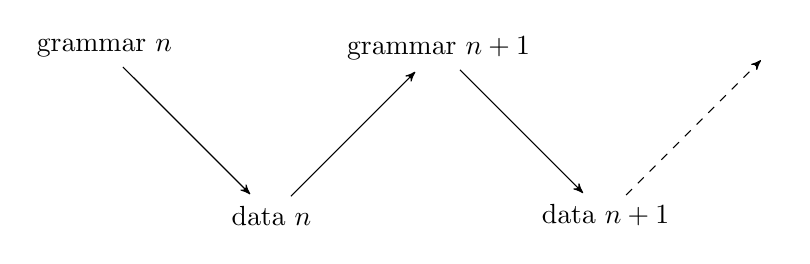
\begin{tikzpicture}[->,>=stealth',shorten >=1pt,auto,node distance=3cm]
  \node (A)      {grammar $n$};
  \node (B) [below right of=A]  {data $n$};
  \node (C) [above right of=B] {grammar $n+1$};
  \node (D) [below right of=C] {data $n+1$};
  \node (E) [above right of=D] {};
\path[->] (A)  edge node {} (B)
  (B) edge node {} (C)
  (C) edge node {} (D)
  (D) edge[dashed] node {} (E);
\end{tikzpicture}
\end{center}
\caption{The iterated process of language acquisition and use}
\label{second}
\end{figure}


\appendix

\chapter{Equilibria}

\chapter{Dynamics}


% \chapter{Notes}
% 
% Intralinguistic and extralinguistic variation factors in Old French negation with ne-¯, ne-mie, ne-pas and ne-point across different text types
% 
% The Spread of Change in French Negation (Grives-Smith)
% 
% 
% We can scrape from this:
% \begin{verbatim}
%      http://artfl-project.uchicago.edu/content/general-overview
% \end{verbatim}
% But, these are not all available texts, but rather a selection that was thought to be representative of "good" French (Grieves-Smith, p. 125)
% 
% As described in the previous chapter, the corpus that we have does not include examples of ne ... pas, ne ... point or ne ... mie used for literal reference, scalar denial or emphatic denial. I therefore tagged each instance of sentence negation for the features predicate negation, proposition denial and presupposition denial. (p.134)
% 
% Englishman John Palsgrave, who published a grammar in 1530. He wrote (Palsgrave 1530: 110):
% For where as they put ne before theyr verbes, so often as they expresse negation, like as we use 'nat' in our tong after our verbes. They put also after theyr verbes pas, poynt or mye, whiche of theym selfe signifye nothyng, but onely be as signes of negation.
% 
% Brinton (2005, 2008)
% 
% Martineau Morgon p.137
% In sum, our findings for the eighteenth-century corpora lead us to hypothesize that in eighteenth-century popular spoken French the rate of ne deletion rose only modestly and that it started in sentences with a clitic subject. In other words, if we consider, along with Schwegler (1988), that deletion of the preverbal negator is the final stage in the cyclical evolution of negation in Romance languages, our findings suggest that, as far as French is concerned, the starting point of this ultimate stage is sentences with a subject clitic. The fact that clitic subjects can be phonetically weakened and are unstressed may be the reason for this.
% 
% The hypothesis that the social and structural diffusion of ne deletion has proceeded at a faster pace in Quebec than in France is consistent with the fact that in the late twentieth century, ne deletion was found to be almost categorical in all syntactic contexts and in the speech of different social groups in Quebec French, but was still associated with differential patterns of structural, social, and geographic diffusion in European French, (see Pohl 1975, Sankoff \& Vincent 1977, Ashby 1981, and Coveney 1996).41
% 
% (1) 9th to 13th centuries: stable period (ne is used alone or is reinforced by words like pas or point that do not have yet a negative meaning; subject clitics are optional) (2) 14th to 16th centuries: unstable period (ne is vying with ne . . . pas/point to
% express negation; PRO drop is on the decrease)
% (3) 17th and 18th centuries: stable period (ne . . . pas/point is firmly established as
% the expression of negation; PRO drop is exceptional)
% (4) 19th and 20th centuries: unstable period (ne . . . pas and pas are vying with
% each other, with pas eventually winning out; affixation of subject clitics is firmly established).53
% 
% p.146
% 
% 
% Interestingly, Eckardt (2007: 257-260) observes that in her data, point 'displays the most varied sample of "puzzling" uses.' On this basis, she suggests that by the time of Classical French, ne ... point may have been the last grammaticized negator to lose its 'emphatic' status, consistent with the findings of Catalani (2001). As I will discuss in the Results chapter, this is confirmed in the present study.
% 
% Before metanalysis, the negative meaning is attributed to the preverbal particle ne, and the emphatic function is attributed to the postverbal element (pas, personne, etc.). From the point of view of the postverbal element, negation is a contextual feature while emphasis is an inherent feature. However, as has been argued by a number of linguists (e.g. Schwegler 1988: 36, Giv�n 1979, ch. 3), negative utterances are more likely to be emphatic in actual use than positive ones; that is, there is a high degree of correlation between negation and emphasis. This correlation sets the condition for metanalysis: since the emphatic element is found frequently in negative contexts, and negative contexts are frequently emphatic, there is a swapping of the two functions: the negative function is attributed to the emphatic element, while the emphatic function is attributed to the nonlinguistic context.
% 
% Croft p.130
% 
% 
% Traugott (1989) and others argue that semantic change typically proceeds gradually through polysemy and ambiguity, driven by the conventionalization of pragmatic inferences. She identifies three tendencies of semantic change based on her investigation of English modal auxiliaries (1989: 34-35):
% \begin{enumerate}
% 	\item Meanings based in the external described situation $>$ meanings based in the internal (evaluative/perceptual/cognitive) described situation.
% 	\item Meanings based in the external or internal described situation $>$ meanings based in the textual and metalinguistic situation.
% 	\item Meanings tend to become increasingly based in the speaker's subjective belief state/attitude toward the proposition.
% \end{enumerate}
% %Tendency I: 
% %Tendency II: 
% %Tendency III: 
% 
% %\pagebreak
% %
% %Evil kings from evil crowns\\
% %ships of water watered down\\
% %To sing is to love, to love to know\\
% %without words or thoughts incurred\\
% %
% %Brilliant things to brilliant ends\\
% %Mother, father, great immortal when\\
% %To know is to go, to go comprehend\\
% %without words or thoughts incurred\\
% %
% %There and then, from here and now\\
% %Facts and figures figured out\\
% %To comprehend's to find, to find to move\\
% %without words or thoughts incurred\\
% %
% %Hymns and hums, to his and hers\\
% %Cousin, daughter, best to listen first\\
% %To move is to live, to live to sing\\
% %without words or thoughts incurred\\
% %


% And the bibliography

\bibliographystyle{mcbride}
\bibliography{diss}

\end{document}


